\chapter{Интеллектуальных анализ данных Web-ресурсов}\label{ch:ch5}

\subsubsection{5.1.1}

Studies of political polarization in social media demonstrate mixed evidence for whether discussions necessarily evolve into left and right ideological echo chambers. Recent research shows that, for political and issue-based discussions, patterns of user clusterization may differ significantly, but that cross-cultural evidence of the polarization of users on certain issues is close to non-existent. Furthermore, most of the studies developed network proxies to detect users’ grouping, rarely taking into account the content of the Tweets themselves. Our contribution to this scholarly discussion is founded upon the detection of polarization based on attitudes towards political actors expressed by users in Germany, the USA and Russia within discussions on inter-ethnic conflicts. For this exploratory study, we develop a mixed-method approach to detecting user grouping that includes: crawling for data collection; expert coding of Tweets; user clusterization based on user attitudes; construction of word frequency vocabularies; and graph visualization. Our results show that, in all the three cases, the groups detected are far from being conventionally left or right, but rather that their views combine anti-institutionalism, nationalism, and pro- and anti-minority views in varying degrees. In addition to this, more than two threads of political debate may co-exist in the same discussion. Thus, we show that the debate that sees Twitter as either a platform of ‘echo chambering’ or ‘opinion crossroads’ may be misleading. In our opinion, the role of local political context in shaping (and explaining) user clusterization should not be under-estimated.

\subsubsection{5.1.2}

The media are normatively expected to play significant roles in conflictual discussions within national and international communities. As previous research shows, digital platforms make scholars rethink these roles based on media behavior in online communicative environments as well as on the structural limitations of the platforms. At the same time, traditional dichotomies between information dissemination and opinion formation roles, although seemingly universal, also vary across cultures. We look at four recent conflicts of comparable nature in the United States, Germany, France, and Russia to assess the roles that legacy media have performed in the respective ad hoc discussions on Twitter. Our approach differs from previous studies, as we combine content analysis of tweets by the media and journalists with the resulting positions of the media in the discussion graphs. Our findings show that, despite the overall trend of the “elite” and regional media sticking to information dissemination, online-only media and individual journalists vary greatly in their normative strategies, and this is true across countries. We also show that combining performance in content and social network analysis may allow for reconceptualization of media roles in a more flexible way.

\subsubsection{5.1.3}

\textit{Background.} Public discussions on social networks have trans-border and multilingual nature. This is especially true for conflictual discussions that reach global trending topics. Being part of the global public sphere, such discussions were expected by many observers to become horizontal, all-involving, and democratically efficient. But, with time, criticism towards the democratic quality of discussions in social media arose, with many works discovering the patterns of echo chambering in social networks. Even if so, there is still scarce knowledge on how affective hashtags work in terms of user clusterization, as well as on the differences between emotionally ‘positive’ and ‘negative’ hashtags. \textit{Objectives.} We address this gap by analyzing the Twitter discussion on the \textit{Charlie Hebdo} massacre of 2015. In this discussion, the Twittershpere has created \#jesuischarlie and \#jenesuispascharlie -- two discussion clusters with, allegedly, opposite sentiments towards the journal’s ethics and freedom of speech. \textit{Research design.} We were interested in whether echo chambers formed both on the hashtag level (based on language use) and within a language (based on user sentiment of French-speaking users). For data collection, we used vocabulary-based Twitter crawling. For data analysis, we employed network analytics, manual coding, web graph reconstruction, and automated sentiment analysis. \textit{Results.} Our results show that \#jesuischarlie and \#jenesuispascharlie are alike in language distribution, with French and English being the dominant languages and the discussions remaining within the Euro-Atlantic zone. The language-based echo chambers formed in both cases. But if \#jesuiuscharlie was a clear sentiment crossroads, \#jenesuispascharlie was a negative echo chamber, thus allowing us to draw conclusions about multi-layer echo chambering.

\subsubsection{5.1.4}

\textit{Ad hoc} discussions have been gaining a growing amount of attention in scholarly discourse. But earlier research has raised doubts in comparability of \textit{ad hoc} discussions in social media, as they are formed by unstable, affective, and hardly predictable issue publics. We have chosen inter-ethnic conflicts in the USA, Germany, France, and Russia (six cases altogether, from Ferguson riots to the attack against \textit{Charlie Hebdo}) to see whether similar patterns are found in the discussion structure across countries, cases, and vocabulary sets. Choosing degree distribution as the structural proxy for differentiating discussion types, we show that exponents change in the same manner across cases if the discussion density changes, this being true for neutral vs. affective hashtags, as well as hashtags vs. hashtag conglomerates. This adds to our knowledge on comparability of \textit{ad hoc} discussions online, as well as on structural differences between core and periphery in them.

\subsubsection{5.2.1}

In this paper authors carry out the research of three different topic models in the context of analyzing different large scale twitter ad hoc discussions, obtained from social network on different social and political events. An experiment is being conducted to test the effectiveness of models in analyzing three known discussions: the riots in Biryulyovo (Russia), Ferguson unrest (USA), Charlie Hebdo shooting (France). The results of the experiment show that the BTM topic model in terms of both Umass and Npmi, yielded the best results on all discussions in comparison to the baseline LDA model and another model for short unbalanced texts -- WNTM.

\subsubsection{5.2.2}

The paper is dedicated to solving the problem of optimal text classification in the area of automated detection of typology of texts. In conventional approaches to topicality-based text classification (including topic modeling), the number of clusters is to be set up by the scholar, and the optimal number of clusters, as well as the quality of the model that designates proximity of texts to each other, remain unresolved questions. We propose a novel approach to the automated definition of the optimal number of clusters that also incorporates an assessment of word proximity of texts, combined with text encoding model that is based on the system of sentence embeddings. Our approach combines Universal Sentence Encoder (USE) data pre-processing, agglomerative hierarchical clustering by Ward’s method, and the Markov stopping moment for optimal clustering. The preferred number of clusters is determined based on the “e-2” hypothesis. We set up an experiment on two datasets of real-world labeled data: News20 and BBC. The proposed model is tested against more traditional text representation methods, like bag-of-words and word2vec, to show that it provides a much better-resulting quality than the baseline DBSCAN and OPTICS models with different encoding methods. We use three quality metrics to demonstrate that clustering quality does not drop when the number of clusters grows. Thus, we get close to the convergence of text clustering and text classification.

\subsubsection{5.2.3}

\textit{Background.} Topic modelling is a method of automated probabilistic detection of topics in a text collection. Use of topic modelling for short texts, e.g. tweets or search engine queries, is complicated due to their short length and grammatical flaws, including broken word order, abbreviations, and contamination of different languages. At the same time, as our research shows, human coding cannot be perceived as a baseline for topic quality assessment. \textit{Objectives.} We use biterm topic model (BTM) to test the relations between two topic quality metrics independent from topic coherence with the human topic interpretability. Topic modelling is applied to three cases of conflictual Twitter discussions in three different languages, namely the \textit{Charlie Hebdo} shooting (France), the Ferguson unrest (the USA), and the anti-immigrant bashings in Biryulevo (Russia), which represent, respectively, a global multilingual, a large monolingual, and a mid-range monolingual type of discussions. \textit{Method.} First, we evaluate the human baseline coding by providing evidence for the Russian case on the coding by two pairs of coders who have varying levels of knowledge of the case. We then measure the quality of modelling on the level of topics by looking at topic interpretability (by experienced coders), topic robustness, and topic saliency. \textit{Results.} The results of the experiment show that: 1) the idea of human coding as baseline needs to be rejected; 2) topic interpretability, robustness, and saliency can be inter-related; 3) the multilingual discussion performs better than the monolingual ones in terms of interdependence of the metrics. \textit{Conclusion.} We formulate the idea of an ‘ideal topic’ that rethinks the goal of topic modelling towards finding a smaller number of good topics rather instead of maximization of the number of interpretable topics.

\subsubsection{5.2.4}

Topic modelling is a technique widely used today to detect hidden topicality of text corpora, including those from social media. But, for many quite widespread online languages, like, e.g., Russian, topic modelling is still used rarely. For the Russian Twitter, only a handful of works exists, and these works lack substantial discussion on topic interpretability. Also, the impact of various properties of texts upon the modelling results remains widely unexplored. We partly cover these gaps by assessing a mid-range text corpus of a conflictual Twitter discussion in two respects. In continuation to our earlier study that applied three topic modelling algorithms (LDA, WNTM, and BTM) and assessed their quality via automated means, we here juxtapose automated assessment to human coding and link the human evaluation of topic quality to sentiment of the topics. We show that human coding disagrees with the results of the objective metrics in the number of interpretable topics, showing slightly higher interpretability for the LDA algorithm, but inter-coder reliability is much higher for BTM. We discuss a range of coding issues true for all the three topic models. We also find that interpretability of a topic by the human coders is linked to presence of negative keywords among the topic descriptors, with the strongest linkage shown by BTM.

\subsubsection{5.2.5}

The linkages between intensity and topicality of online discussions, on one hand, and those of offline on-street political activity, on the other hand, have recently become a subject of studies around the world. But the results of quantitative assessment of causal relations between onsite and online activities of citizens are contradictory. In our research, we use conflicts with violent trig-gers and the subsequent lines of events that include street rallies, political manifestations, and/or peaceful mourning, as well as public political talk, to trace the pivotal points in the conflict via measuring Twitter content. We show that in some cases Granger test does not work well, like in the case of Cologne mass harassment, for detecting the causality between online and onsite activities. In order to suggest a way to qualitatively assess the linkages between online and offline activities of users, we deploy topic modeling and further qualitative assessment of the changes in the topicality to link the topic saliency to the time of offline events. We detect several periods with varying topicality and link them to what was going on in the offline conflict.

\subsubsection{5.2.6}

Topic modeling is a method of automated definition of subtopics in a text corpus. Usage of topic modeling for short texts, e.g. tweets, is highly complicated due to their short length and grammatical restructuring, including broken word order, abbreviations, and contamination of different languages. In this paper, the authors use the BTM topic modelling algorithm (previously found to work best in comparison with two other topic models measured by automated coherence metrics Umass and NPMI) to test three topic quality metrics independent from topic coherence. Topic modelling is applied to three cases of ethnic conflict discussions on Twitter in three different main languages, namely the Charlie Hebdo shooting (France), the Ferguson unrest (the USA), and the anti-immigrant bashings in Biryulevo (Russia), thus combining a large multilingual, a large monolingual, and a mid-range monolingual type of discussion. We measure the quality of modeling by looking at topic interpretability, topic robustness, and topic saliency. The results of the experiment show that the three topic features may be interdependent (but not always are); the multilingual discussion performs better than the monolingual ones in terms of interdependence of the metrics and formation of ideal topics; and interpretability does not depend on multi-/monolingualism and the dataset volume.

\subsubsection{5.2.7}

\paragraph{EN} In this paper, the authors consider two topic models LDA (Latent Dirichlet Allocation) and WNTM (Word Network Topic Model), which rely on statistical data on the co-occurrence of words within the text, to identify topics in the problem of analysing the corpus of short texts. An experiment is conducted in which a comparative analysis of these models is made on the well-known test collection News and a set of data consisting of messages from users of the social network Twitter with the hashtag Biryulyovo. The results of the experiment show that the WNTM model, specialized for working with short texts, is more effective than the base model (LDA) on all the data presented for all performance measurements used.

\paragraph{RU} В данной работе авторы рассматривают две тематические модели LDA (Latent Dirichlet Allocation) и WNTM (Word Network Topic Model), которые опираются на статистические данные о совпадениях слов внутри текста, для выявления тем в задаче анализа корпуса коротких текстов. Ставится эксперимент, в котором проводится сравнительный анализ данных моделей на известной тестовой коллекции News и наборе данных, состоящих из сообщений пользователей в социальной сети Twitter по хэштегу Бирюлево. Результаты эксперимента показывают, что специализированная модель WNTM для работы с короткими текстами, имеет большую эффективность на всех представленных данных по сравнению с базовой моделью (LDA) по всем представленным критериям.

\subsubsection{5.3.1}

Over the past few years the sentiment analysis task of users' posts in social networks has become very popular among researchers. In this paper, authors present and describe the developed multi-lingual knowledge-based approach of sentiment analysis in major conflict ad hoc discussions of the social network Twitter. An experiment is made in which the quality of the proposed method is evaluated with different parameters on two real ad hoc discussions: Ferguson unrest (USA) and Biryuliovo bashings (Russia). The results of the experiment show a good quality of the sentiment analysis of the discussions. In particular, the average value of the accuracy of Russian and English is 0.65, and the f-measure is 0.7.

\subsubsection{5.3.2}

\textit{Background.} The spread of affective content on social media, as well as user grouping based on affect \cite{Papacharissi}, has been a focus of scholarly attention for over a decade. But, despite this, we lack evidence on what roles various particular emotions play in the dynamics of discussions on social media. Emotional contagion theory (Hatfield et al. 2014) adapted for social media suggests that diffusion of emotions happens on individual level, via direct one-time contact with emotionalized content \cite{CovielloSohnKramer}. Other theories, like theories of social influence or social learning \cite{Young}, thought, suggest multiple, hierarchical, and/or topically-restricted contacts. The idea of affective agenda \cite{ColemanWu} implies that the dynamics of an emotional discussion needs to be assessed on the aggregate level. The question remains -- what role the emotions taken on aggregate level play in the discussion dynamics, being either catalyzers or inhibitors of the discussions. One may suggest that emotions of different stance (positive/negative) may spur/slow down the discussions in various ways. \textit{Objectives.} We analyze the spread of two polar emotions -- anger and compassion -- in three Twitter discussions on inter-ethnic conflicts, namely Ferguson protests (the USA, 2014), Charlie Hebdo massacre (France, 2015), and mass harassment in Cologne (Germany, 2015--2016). By analyzing the co-dynamics of the overall discussions and these two emotions we can conclude whether the pattern of the spread of emotions and its link with the discussion dynamics is the same in various language segments of Twitter. \textit{Data collection and methods.} The data we use were collected by our patented Twitter crawler in the aftermath of the conflicts and include altogether over 2,5 M tweets. We used manual coding by native speakers and machine learning to detect the emotions; then, we visualized the dynamics of growth of the emotional content of the discussions and used Granger test to see whether anger or compassion gave a spur to the discussions. \textit{Results.} We have received moderate results in terms of the dependence of the number of neutral users upon that of emotional users, but have spotted that the beginnings of the discussions, as well as the discussion outbursts, depend more on compassion, not on angry users, which needs more exploration. We have also shown that the hourly dynamics of emotions replicates that of the larger discussion, and the numbers of angry and compassionate users per hour highly correlate in all the cases.

\subsubsection{5.3.3}

Studies of user sentiment on social networks like Twitter have formed a steadily growing research area. But there is still lack of knowledge on whether the discussion clusters tagged by emotionally opposite hashtags differ in sentiment distribution, both in terms of difference between hashtags and between user types, e.g. non-influencers and influential accounts. We look at two hashtags that marked the discussion on the \textit{Charlie Hebdo} massacre of 2015, namely \#jesuischarlie and \#jenesuispascharlie. As sentiment analysis studies for the French language are rare, we elaborate our own approach to sentiment vocabulary. We apply human coding and machine learning to correct the automated sentiment assessment. Then we apply the enhanced knowledge on sentiment to both discussion segments and compare the configuration of the resulting sentiment-based nebulae in overall and francophone-only discussions. Also, we define influencers for both discussions and compare whether ordinary and institutional users differ by sentiment. We have three notable findings. First, negativity structures \#jenesuispascharie more than \#jesuischarlie. Second, while francophones communicate cross-sentiment inside the francophone talk, their negativity tends to cast impact upon cluster formation inside general discussions. Third, influencers in both cases tend to be more negative than positive, but institutional users bear neutral and positive sentiment more than ordinary people.

\subsubsection{5.3.4}

\paragraph{RU} В последнее десятилетие дискуссии в Интернете, маркированные хэштегами, и участвующие в них социальные группы породили новое и  быстро растущее поле междисциплинарных исследований. Оно связывает изучение общественного мнения, исследования публичной сферы и анализ социальных сетей. Но все эти исследования пока однозначно не ответили, «можно ли найти Хабермаса в Твиттере», -- в силу экспрессивности и недиалогичности коммуникации в социальных сетях, низкого потенциала тематических дискуссий по созданию «перекрестка мнений», а  также языковых границ, препятствующих кросскультурной дискуссии пользователей и  развитию глобальной публичной сферы.

Данное исследование призвано оценить языково-пространственный аспект дискуссий под двумя «аффективными» и  взаимоисключающими хэштегами, отражающими ценностные позиции пользователей Твиттера, -- \#JeSuisCharlie и \#JeNeSuisPasCharlie. Мы оцениваем языковое распределение в коллекциях твитов и распространение хэштег-маркированных обсуждений за пределы французского языка. Для идентификации языковой структуры дискуссии используются автоматизированный веб-краулинг, ручное кодирование коллекций твитов, реконструкция веб-графов, их визуальный и сетевой анализ.

Результаты исследования свидетельствуют о  том, что, несмотря на  разницу в  объеме обсуждения, обе дискуссии имеют сходную языковую структуру, включающую языковообусловленные «эхо-камеры» как на уровне самой дискуссии (особенно для \#JeNeSuisPasCharlie), так и внутри нее; при этом дискуссии не демонстрируют «столкновение цивилизаций» и не являются по-настоящему глобальными. В трансграничных дискуссиях идея «эхо-камер» выходит на уровень национального языка. Мы также показываем, что билингвальные, а не мультилингвальные пользователи являются связующими узлами многоязычной дискуссии.

\paragraph{EN} Within the last decade, hashtag-based publics and various aspects of the discussions produced by them have created a rapidly growing field of interdisciplinary research linking public opinion and public sphere studies to social network analysis. Despite this growth, there is still scarce evidence that ‘Habermas is on Twitter’, due to the affective and non-dialogue nature of expression in social networks, seemingly low capacity of ad hoc discussions to create ‘opinion crossroads’, and language boundaries that prevent, i. a., cross-cultural participation of users in a given discussion and, thus, do not let the global public sphere develop. Having this in mind, we explore the spatial dimension of two affective hashtag-based publics with mutually exclusive value-loaded positions -- \#JeSuisCharlie and \#JeNeSuisPasCharlie. We look at language distribution within the tweet collections and the expansion of the hashtagged discussion to the languages other than French. To trace the discussion outbursts, we use automated web crawling, manual coding of tweet collections, and web graph reconstruction and visual analysis. Our results suggest that, despite the differences in the volume of expression, the language structure of both hashtags was quite similar and formed echo chambers on the level of a hashtag as well as on sub-levels. Also, we see that bilingual but not multilingual users bridge the sub-level echo chambers. We argue that global compassion publics not only lift up the idea of echo chambers to a new level (since ‘national’ language-based echo chambers clearly show up on the discussion graphs) but also revive the concept of spiral of silence.

\subsubsection{5.3.5}

Abstract Today, aggressive verbal behavior is generally perceived as a threat to integrity and democratic quality of public discussions, including those online. However, we argue that, in more restrictive political regimes, communicative aggression may play constructive roles in both discussion dynamics and empowerment of political groups. This might be especially true for restrictive political and legal environments like Russia, where obscene speech is prohibited by law in registered media and the political environment does not give much space for voicing discontent. Taking Russian YouTube as an example, we explore the roles of two under-researched types of communicative aggression -- obscene speech and politically motivated hate speech -- within the publics of video commenters. For that, we use the case of the Moscow protests of 2019 against non-admission of independent and oppositional candidates to run for the Moscow city parliament. The sample of over 77,000 comments for 13 videos of more than 100,000 views has undergone pre-processing and vocabulary-based detection of aggression. To assess the impact of hate speech upon the dynamics of the discussions, we have used Granger tests and assessment of discussion histograms; we have also assessed the selected groups of posts in an exploratory manner. Our findings demonstrate that communicative aggression helps to express immediate support and solidarity. It also contextualizes the criticism towards both the authorities and regime challengers, as well as demarcates the counter-public.

\subsubsection{5.4.1}

Abstractive summarization is a technique that allows for extracting condensed meanings from long texts, with a variety of potential practical applications. Nonetheless, today’s abstractive summarization research is limited to testing the models on various types of data, which brings only marginal improvements and does not lead to massive practical employment of the method. In particular, abstractive summarization is not used for social media research, where it would be very useful for opinion and topic mining due to the complications that social media data create for other methods of textual analysis. Of all social media, Reddit is most frequently used for testing new neural models of text summarization on large-scale datasets in English, without further testing on real-world smaller-size data in various languages or from various other platforms. Moreover, for social media, summarizing pools of texts (one-author posts, comment threads, discussion cascades, etc.) may bring crucial results relevant for social studies, which have not yet been tested. However, the existing methods of abstractive summarization are not fine-tuned for social media data and have next-to-never been applied to data from platforms beyond Reddit, nor for comments or non-English user texts. We address these research gaps by fine-tuning the newest Transformer-based neural network models LongFormer and T5 and testing them against BART, and on real-world data from Reddit, with improvements of up to 2\%. Then, we apply the best model (fine-tuned T5) to pools of comments from Reddit and assess the similarity of post and comment summarizations. Further, to overcome the 500-token limitation of T5 for analyzing social media pools that are usually bigger, we apply LongFormer Large and T5 Large to pools of tweets from a large-scale discussion on the Charlie Hebdo massacre in three languages and prove that pool summarizations may be used for detecting micro-shifts in agendas of networked discussions. Our results show, however, that additional learning is definitely needed for German and French, as the results for these languages are non-satisfactory, and more fine-tuning is needed even in English for Twitter data. Thus, we show that a ‘one-for-all’ neural-network summarization model is still impossible to reach, while fine-tuning for platform affordances works well. We also show that fine-tuned T5 works best for small-scale social media data, but LongFormer is helpful for larger-scale pool summarizations.

\subsubsection{5.4.2}

Agendas in online media have become a scholarly focus nearly two decades ago, leading to shifting conceptualizations of what we see as agenda. Thus, agendas and agenda shifts inside online discussions have shown its potential to influence offline deliberation, aggregate support, fuel protest, passing through and/or bypassing traditional media’s gatekeeping. Real-time (or nearly-real-time) learning about quick agenda movement inside globalized public debate might be particularly important for international organizations like UN or EU. However, we today lack both knowledge on how agendas move in such discussions and instruments on such analysis. In particular, we are next-to-unaware of to what extent globally relevant themes get contextualized within language-based discussion segments, as well as to what extent the latter depend on each other and lag behind each other in developing agendas and public opinion on quickly evolving issues or conflicts. In this paper, we propose a method of agenda detection based on neural-network text summarization and compare summaries of tweet packages across three languages within the Twitter hashtag \#jesuischarlie. We show that sentiment detection may allow for quality assessment of the text summaries, as compared to aggregated sentiment to the original tweets. We show that, outside France, agendas were more interpretational, abstract, and non-contextualized. The pattern of news changing to ‘issue outburt’ was simultaneous in dense discussion segments and lagged behind in a sparser one. We also show that, globally, main issues of the discussion may be spotted within the first hour.

\section{Анализ Web-графов}\label{sec:ch5/sect1}

\subsection{Beyond left and right: Real-world political polarization in twitter discussions on inter-ethnic conflicts}\label{subsec:ch5/sec1/sub1}

\subsubsection{1. Introduction}

Today, social polarization is believed to be growing both along traditional and newer lines along which schisms form \cite{DucaSaving}, of which political ones are, arguably, the sharpest. Despite the ever-increasing body of knowledge on political attitudes and alignments online, we still lack understanding of how political divisions show up in issue-oriented discussions and whether there is a cross-country pattern.

Despite all the well-described representation distortions \cite{Daniels}, the content of social media is still used for predicting consumer and/or electoral choices \cite{ColleoniRozzaArvidsson}, and the studies of political polarization on social media, including Twitter, are growing in popularity \cite{Barbera}. However, there are several shortcomings in today’s studies of political polarization in user-generated content.

Thus, in most cases, audience polarization is studied by examining purely political issues or events, while social conflicts of race, gender or religious origins with both evident and idiosyncratic polarization and politicisation \cite{McCrightDunlap} are rarely studied. Due to context and language differences, multi-country studies are also rare, especially where both established democracies and countries beyond the Euro-Atlantics are included, as, for most observers, these remain politically incomparable. However, conditions other than political regimes may create grounds for cross-cultural juxtapositions \cite{BodrunovaLitvinenkoBlekanov,BodrunovaBlekanovMaksimov}.

Another conceptual limitation is that, even in the most advanced studies, the detection of users’ political affiliations or ideologies is done via proxies, most often via structural network factors, such as: friendship affiliations; patterns of following \cite{BarberaJostNagler,Rivero}; or content sharing \cite{ColleoniRozzaArvidsson}, which could be misleading. Addressing this gap, newer works show that group polarization in social media may be studied by looking at user texts, including complex referrals to specific phenomena that matter for group identity \cite{Evolvi}. We argue that the analysis of political divisions needs to unite both structural and content aspects \cite{Bodrunova}.

In order to bridge these gaps in previous studies, we look at Twitter discussions regarding inter-ethnic clashes; they have similar conflict triggers and structure of social groups involved into conflict \cite{BodrunovaLitvinenkoBlekanov2017}. Whilst avoiding making straightfor- ward comparisons, we explore users’ political polariza- tion and suggest a mixed method to detect it across three cases in different political regimes: the USA; Germany; and Russia. By the UN estimates of 2013–2017, these countries have recently been the three most attractive countries to migrants in the world \cite{UN2013,UN2017} and have all witnessed violent inter-ethnic clashes that became global trending topics on Twitter.

This article, thus, is organized as follows: In Section 1, we review the approaches of assessing user polarization on social media and the conflicts under our scrutiny. In Section 2, we formulate the research questions and describe our methodology. In Section 3, we provide the results; in Section 4, we interpret and discuss them.

\subsubsection{2. Political Polarization on Twitter: The Current State of Research}

\paragraph{2.1. Political Polarization Studies and the Current Research Gaps}

Throughout recent years, mixed evidence has persisted in social media studies on whether users go online to agree or to argue \cite{YardiBoyd}. Research into echo chambers \cite{ColleoniRozzaArvidsson,Sunstein2002} has shown that user homophily, both structurally and semantically, may prevent the formation of online ‘opinion crossroads’, as there is ‘evidence of persistent ideological sorting in online communication networks’ \cite[p.~2]{Barbera}. However, a range of works point to the opposite effects in Twitter communication, with weaker ties responsible for the diversification of the consumption of political information \cite{Barbera} as well as different platform features on Twitter leading simultaneously to echo chambers and inter-community communication \cite{ConoverRatkiewiczFrancisco}. Thus, evidence suggests more research is needed to assess the patterns of users’ political clusterization on social networks.

Until today, most Twitter polarization studies are bound to the one-country-one-case strategy -- with a few notable exceptions \cite{Barbera,BarberaJostNagler}. Another problem arises from today’s understanding of online political polarization \cite{BramsonGrimSinger} as a situation when ‘a social or political group is divided into two opposing sub-groups having conflicting and contrasting positions, goals and viewpoints, with few individuals remaining neutral or holding an intermediate position’ \cite[p.~215]{CalaisGuerraMeiraJrCardie} \cite{Isenberg,Sunstein2002}.

Empirical evidence suggests that, if a heterogeneous group containing users with two opposing views has a non-zero cross-view retweet rate, it will end up as two polarized communities \cite{ConoverRatkiewiczFrancisco}. Following this logic, the studies of political polarization result in pre- defined binary descriptions of polarized communities -- see \cite{MoralesBorondoLosada} for Venezuela; 
\cite{AgathangelouKatakisRori} for Greece; or \cite{WeberGarimellaBatayneh} for Egypt.

However, for studies beyond the two-party electoral process, it seems useful to remember that polarization is an individual case of clusterization along schismatic lines, disregarding the number of resulting clusters \cite{EstebanRay}. In social conflicts, conflicting groups are not necessarily structured along binary political party divisions. The classic work of \cite{TajfelTurnerAustin} shows how social identity (including ethnic identity) divides in- and out-groups, while a later normative model of dissent in social groups \cite{Packer} implies that, in inter-ethnic conflicts, the majority may divide into pro- minority and anti-minority clusters if the anti-minority at- titude is perceived as harmful to the collective \cite[p.~5]{PackerChasteen}. Also, the very political spectra may be highly multi-dimensional, as The Manifesto Project (https://manifesto-project.wzb.eu/) or Polity Project (http://www.systemicpeace.org/polity/polity4.htm) suggest. Thus, we consider polarization more as multi-polar fragmentation of divergent clusters, of which bipolar clusterization is just an option.

Non-bipolar clusterization seems to be especially probable for ‘issue’ or ‘ad hoc’ publics \cite{BrunsBurgess,Papacharissi} that emerge on social networks. This claim is supported by research on the topic and issue-based discussions \cite{ElgesemSteskalDiakopoulos}. In single case studies, user polar- ization has been studied in regard to abortion, same-sex marriage, gun control, and climate change \cite{Elgesem,CalaisGuerraMeiraJrCardie,YardiBoyd}, with varying degrees and directions of polarization detected. Moreover, there is a clear difference in polarization patterns between political and non-political issues \cite{BarberaJostNagler}. But the evidence of differences in polarization patterns is still scarce in academic literature.

The biggest challenge in today’s polarization studies is that instead of taking into account the actual content of user posts, detection of users’ political affiliations is conducted via proxies. Of those, the most interesting results come from assessing structural network factors such as friendship affiliations \cite{BarberaRivero}, retweeting patterns \cite{CalaisGuerraVelosoMeiraJr}, patterns of political following \cite{BarberaJostNagler,Rivero} or content-sharing patterns \cite{AdamicGlance,BakshyMessingAdamic,ColleoniRozzaArvidsson,Elgesem}. However, using proxies may be misleading \cite{AdamicGlance} and even express analysis of actual tweets shows the extreme diversity of political views, both in the form of direct expression and in opinionated content.

However, if not proxies, then what? Several studies suggest that group polarization in social media may be examined by analysing complex user referrals to phenomena that matter for their identity and group alignment \cite{Evolvi}, as it is how the attitudes are expressed in natural language. In the simplest possible terms, one would take user attitudes (positive, negative, and neutral) towards particular objects for such referrals.

Thus, we will try to construct group divisions from the actual Tweet content by coding user referrals towards political players and then defining which of these attitudes divide the users most, and for how many clusters.

\paragraph{2.2. Lexicon-Based Approaches to the Analysis of User Polarization}

The area of research closest to our idea of bringing content into polarization studies is a lexicon-based analysis of Twitter data. In recent years, the field has experienced explosive growth, predominantly based on the analysis of sentiments. Without delving fully into these methodologies, we will simply note that the possibility of use of vocabulary-based approaches for polarization assessment tasks \cite{HillmanTrier} is usually based on combining lexical and structural analysis. Several researchers went beyond so-called ‘naïve’ sentiment and have tried to link affect \cite{StieglitzDangXuan} or appraisal \cite{DangXuanStieglitzWladarsch} in user texts, types of lexical units \cite{SperiosuSudanUpadhyay}, and structural elements of Twitter discussions, like graphs of following or speed and volume of Tweet dissemination. Using these and other works, one could conclude that a sentiment-based approach to detecting left and right differences would imply developing a ‘negative’ (say, leftist) + neutral + ‘positive’ (say, rightist) lexicon and applying them to the discussion bulk. However, the problem that we have run into with this approach is the following:

\begin{enumerate}
	\item The users expressed not ‘left views’ or ‘right views’ but attitudes (with their lexical markers) towards politicians, institutions, social groups, or events (‘actors’);
	\item A given user would express attitudes towards not just one but many actors of different political stances;
	\item The same user could express recognized- as-rightist attitudes towards one actor and recognized-as-leftist attitudes towards another actor of comparable significance (e.g., immigrants and nationalists);
	\item The same user could express negative views on both leftist and rightist actors (say, Barak Obama and the KKK in the USA).
\end{enumerate}

In case 3, the user’s preferences, as measured by one-dimensional positive/negative sentiment analysis, would create a zero-sum, and assigning the bias would not be possible. In case 4, an at least two-dimensional measurement of the political spectrum is needed. Taking this into consideration, we have further developed our research questions and the exploratory research design based on user sentiment, but not on pre-defined target-independent lexicons. Instead, to better capture user attitudes, we will use expert coding of Tweets, standardising the coding process with the help of the idea of ‘complex user referrals’ by Evolvi (2017) \cite{Evolvi}.

\paragraph{2.3. The Research Cases}

As stated above, we have studied three intergroup conflicts of ethnic or racial origins in the three leading immigration recipient countries: the USA, Germany, and Russia. Direct comparisons of ad hoc discussions \cite{BrunsBurgess} are currently viewed with some doubt in academic literature. Without developing a strictly com- parative research design, we have argued elsewhere \cite{BodrunovaLitvinenkoBlekanov2017,BodrunovaBlekanovMaksimov} that the conflicts we picked for the analysis are similar enough as research cases. They share a range of attributes: a violent interpersonal trigger, outbursts of public discussion across media platforms (becoming trending topics on Twitter), social polarization along the inter-ethnic or inter-race chasms, street action, and involvement of federal authorities. In addition, they were chosen because they were the first in a line of similar conflictual cases and, at least partly, set the communicative patterns for later discussions.

The cases are described as follows:
\begin{enumerate}
	\item A violent uprising against immigrants from Central Asia in the district of Biryulyovo, Moscow, Russia, in September 2013. After immigrant Orkhan Zeinalov, allegedly, killed local youngster Egor Scherbakov, the Biryolyovo residents destroyed the local warehouse and a trade centre around which hundreds of illegal immigrants had been dwelling. Several non-violent ‘people’s gatherings’ followed.
	
	\item Ferguson riots, Missouri, USA, in August 2014. There, unarmed African American teenager, Mike Brown was shot to death by white police officer Darren Wilson. The killing, as well as the defensive behaviour of the local police department, spurred several waves of street protests and peaceful support actions, including crowds at Mike Brown’s funeral ceremony.
	
	\item Mass harassment and rape of females on New Year’s Eve of 2016 in Cologne, Germany. Over 1,000 women reported being harassed during the celebrations on the city’s main square, allegedly, by re-settlers from North Africa and the Middle East. After that, demonstrations in protest were organized by radical political actors (PEGIDA movement and the party ‘Alternative for Germany’).
\end{enumerate}

\subsubsection{3. Research Questions and Methodology}

\paragraph{3.1. The Outline of the Research Design}

\paragraph{3.1.1. Research Questions} From what was said above, we have formulated the fol- lowing research questions:

\paragraph{RQ1. How, if at all, do the users cluster within the discussions, based on their attitudes to the major conflict actors? Does binary clusterization best describe user grouping?}

\paragraph{RQ2. Can the clusters be described as left or right in relation to the respective national political spectra? If not, then how could these clusters be described?}

\paragraph{RQ3. Are there similarities in the cluster structure of the discussions?}

\paragraph{3.1.2. The Research Design}

The way the RQs were formulated demanded an exploratory research design. To answer the research questions, we had to see which user groups emerged among the influencers and what discourses they conveyed.

Our concept for detecting user polarization was that political grouping within a discussion was constructed via a multi-dimensional combination of attitudes towards political actors (as defined above). These major political actors needed to be deduced from the discussions themselves. Then, the attitudes towards these players would be decrypted by expert coders for the key users, or influencers \cite{BodrunovaBlekanovMaksimov}, usually the bearers of the spectrum of attitudes.

The data received after coding would undergo clusterization, with each user belonging to one non-fuzzy cluster. Tweets by the users in the detected clusters would provide the word frequency vocabularies, which, after expert assessment, would turn into clusterization vocabularies. The latter would then be applied to all the users in the discussions, to see which users get into clusters and which discourses form there.

This approach, even if simple enough and reliant on expert intrusion, allows us to take into account the nature of the users’ political discussion, as well as the lack of linearity of their political positioning. We consider this crucial for studies on conflict discussions, as it may allow the inclusion of conflict-invoked (e.g., pro- or anti- minority), actor-oriented (e.g., authorities), and traditional political divisions (e.g., left and right and centre and radical). At this exploratory stage, our method does not imply machine learning or supervised approaches to data classification; we use big datasets at this stage of data collection only.

\paragraph{3.2. The Research Procedures}

\paragraph{3.2.1. Data Collection and Pre-Processing}

As this work is part of a bigger research project, our methods of data collection were described in detail previously \cite{BodrunovaLitvinenkoBlekanov2017}. Here, we briefly describe the steps we followed.

We used trendinalia.com to detect the initial discussion keywords and snowball reading to amplify this collection, thus forming the vocabularies for crawling. Trendinalia.com is a web service that allows daily monitoring of both world, regional, and national Twitter trending hashtags and words with no hashtag on an hourly basis, with the possibility of backdating; it has worked best in terms of detecting the trending topics, compared to the over ten other websites we had tried since 2013.

Using an API-independent Twitter crawler \cite{BlekanovSergeevMartynenko}, we collected the content of the discussions. All publicly available Tweets and the data on user interactions (likes, retweets, comments) were collected by a two-step procedure. Step one in- cluded the users who posted under the hashtags. Step two detected a wider community of likers, retweeters and commenters. On the discussion graph, only the step one nodes have been visualized.

Due to reasons regarding feasibility and sample comparability, collection periods differed. Thus, for Russia and Germany, the download period was 30 days after the trigger event. For the USA, we had to select the two weeks following the shooting, with Mike Brown’s funeral as the central event. The user samples included:

\begin{itemize}
	\item For Biryulyovo -- Step1: over 3,700 users; Step2: over 12,000 users;
	\item For Ferguson -- Step1: over 70,000 users; Step2: over 210,000 users;
	\item For Cologne -- Step1: over 12,000 users; Step2: over 99,000 users.
\end{itemize}

\paragraph{3.2.2. Data Analysis}

To answer RQ1, we needed to cluster key users by their political views, define the cluster vocabularies, and apply these vocabularies to the rest of the users, in order to see the discussion clusters and interpret their discourses.

As we expected the influencers to be bearers of the polarizing discourse, for each case, we defined the group of influencers based on nine parameters: the number of Tweets, likes, retweets, comments, in-degree, out- degree, degree, betweenness, and pagerank centralities. After these experiments, using various thresholds, the top 50 users were chosen as the cutting line for each parameter. As many users were repeated in the top due to several specifications, the duplicates were deleted. After elimination of influencers with low numbers of Tweets and bot-like influencers (with a percentage of repeated Tweets over 50\%) 156 users for Germany, 105 users for Russia, and 105 the USA were left. But, for the USA sample (which was several times bigger in the number of Tweets), the number of users was reduced by half, to 52 users. Their respective tweet collections for reading and coding included 13,359, 3,012, and 9,540 tweets.

To define user attitudes towards political actors, we developed scales for coding and coded the users (not their Tweets). The coders were experts in inter-ethnic conflict and, additionally, academic native-speakers, and the level of inter-coder reliability as measured by Cohen’s kappa reached at least 0.68 for any two sub-samples. The coders used the scale from \(-2\) to 2 to assess the attitude of each user to the following groups that had been identified as attitude triggers by reading the tweets before coding: 1) the minority (immigrants or African Americans); 2) ‘radical right’ or ‘radical white’ -- nationalists in Russia, PEGIDA and AFD in Germany, and the Tea Party and the KKK (as a label for radical whites) in the USA; 3) the incumbent country leaders -- Vladimir Putin and Dmitry Medvedev in Russia, Angela Merkel in Germany, and Barak Obama and Hillary Clinton in the USA; 4) local authorities and police forces grouped together as the ‘oppressive and responsible’ actors. Attitudes towards liberal opposition in Russia and to Republicans and Democrats were also coded, as we found them salient in the Tweets.

Based on this coding, the influences were clustered to form groups with similar combinations of attitudes. After clustering, the Tweets of each group were merged, and fully divergent frequency vocabularies of their discourses were formed with the use of expert vocabulary ‘cleaning’. Then, we applied the vocabularies to all the users in the discussions, to see how the discourses distribute within the discussion structure. We also measured whether these discourses formed distinct nebulae; but even if they did not, we assessed which users belonged to these discourses and interpreted the semantics of their speech qualitatively. What mattered for our analysis was whether the influencers formed distinct groups; all the following steps were the consequence.

In detail, the research steps were the following.

\begin{enumerate}
	\item Based on our coding, the influences of each case were grouped with the help of a k-means clustering algorithm with sorted the distances. With the number of clusters and the number of variables being diverse, the best solutions were finally chosen based on Silhouette metric S, within- and between-cluster square sums, examinations of variable means in each cluster (see Figures~\cref{fig:userAttitudesRussia} to~\cref{fig:userAttitudesUSA} for Russia, Germany, and the USA, respectively), and expert reading of tweets in each cluster. All the three influencer groups clustered well; Germany clustered best, Russia followed, and the USA the least, but all the solutions were sufficient by Silhouette from 2 to 10 possible clusters. To identify the best solutions, other aforementioned metrics were used. Those solutions were:
	\begin{itemize}
		\item For Russia: 4 variables (attitude to liberal opposition excluded), 3 clusters of 49, 36, and 20 users, \(S > 0.4\); 
		
		\item For Germany: 4 variables, 3 clusters of 99, 48, and 9 users, \(S > 0.5\);
		
		\item For the USA: 5 variables (attitude to Democrats excluded), 4 clusters of 15, 15, 12, and 10 users, \(S > 0.2\).
	\end{itemize}
	\item For each cluster, word frequency vocabularies were formed by merging the Tweets, ranging the words by frequency, and expert reading. After reading, only the words unique or highly characteristic for each cluster (for example, two mentions in one cluster and 160 in another would result into eliminating the word in the first one and leaving it in the other). If the difference between the numbers of mentions in any two clusters of the case was smaller than ten times, the word was eliminated in all the clusters.
	
	\item We applied the thesaurus to the rest of the users in each case; we wanted to identify the users who use the words from the divergent thesauri. As a result, we have received three types of users in each case: 1) the users who belonged to clusters 1 to 3 or 4; 2) the ‘overlappers’ who used the language of more than one cluster; 3) the users who did not use the discourses (mostly due to a low number of their Tweets). To ensure a higher quality of marking users, rather than using individual words from the thesauri, two-word combinations were used.
	
	\item Based on this information, we constructed the graphs of discourse distribution, with users as apexes and user interactions (comments and/or retweets) as edges, and calculated the indices for user centralities. We assessed who were the most influential discourse bearers and what they spoke about. We used Gephi algorithms OpenOrd and Force Atlas 2 for graph construction (see \cite{MartinBrownKlavans}, on OpenOrd), as the former favours centripetal graphing and the latter better shows visual homophily (see Figures~\cref{fig:openOrdRussia} to~\cref{fig:openOrdUSA}). To see whether the groups bearing the discourses were tighter than inter-group connections, we calculated the mean number of in-group and inter-group edges.
\end{enumerate}

\begin{figure}[ht]
	\centerfloat{
		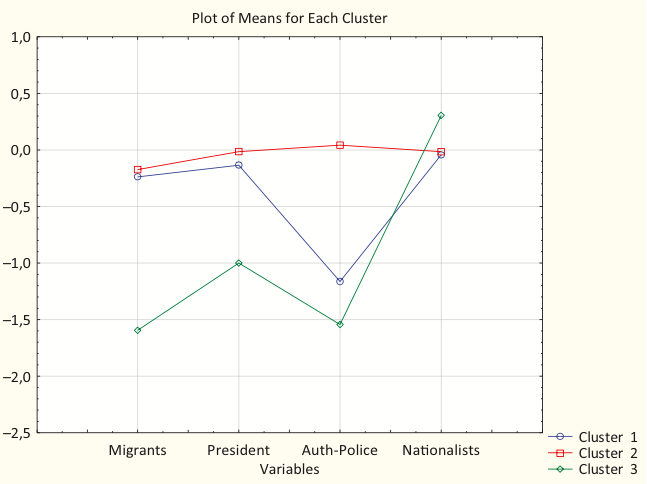
\includegraphics[scale=0.5]{userAttitudesRussia}
	}
	\caption{Mean values of user attitudes to the selected political actors in attitude-based clusters for Russia.}\label{fig:userAttitudesRussia}
\end{figure}

\begin{figure}[ht]
	\centerfloat{
		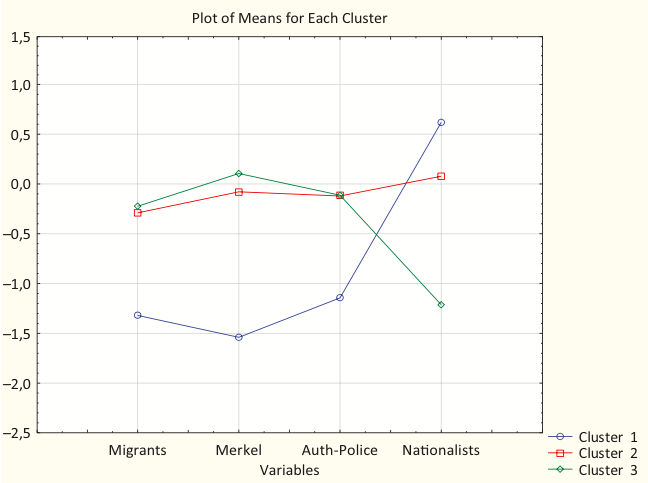
\includegraphics[scale=0.5]{userAttitudesGermany}
	}
	\caption{Mean values of user attitudes to the selected political actors in attitude-based clusters for Germany.}\label{fig:userAttitudesGermany}
\end{figure}

\begin{figure}[ht]
	\centerfloat{
		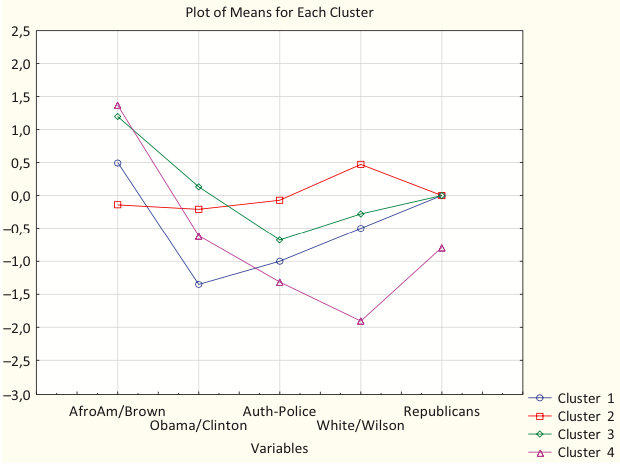
\includegraphics[scale=0.52]{userAttitudesUSA}
	}
	\caption{Mean values of user attitudes to the selected political actors in attitude-based clusters for the USA.}\label{fig:userAttitudesUSA}
\end{figure}

\begin{figure}[ht]
	\centerfloat{
		\hfill
		\subcaptionbox[List-of-Figures entry]{\label{fig:openOrdRussia-1}}{%
			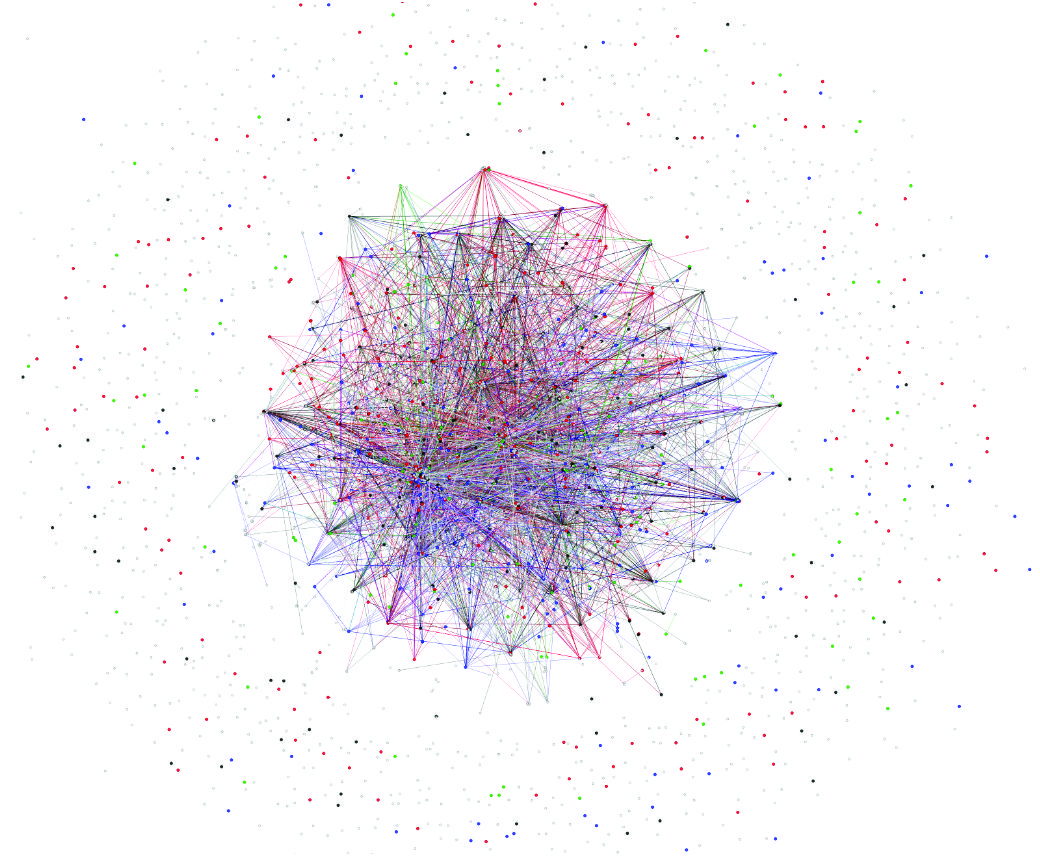
\includegraphics[width=0.419\linewidth]{openOrdRussia1}}
		\subcaptionbox{\label{fig:openOrdRussia-2}}{%
			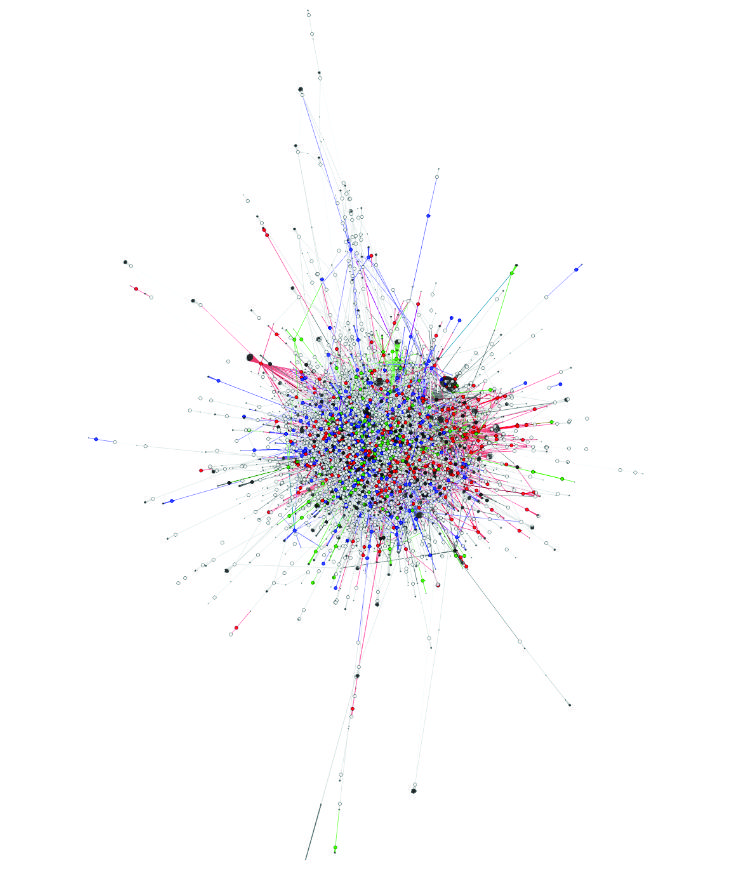
\includegraphics[width=0.4\linewidth]{openOrdRussia2}}
		\hfill
	}
	\legend{Blue: Cluster 1, ‘anti-establishment nationalists’; red: Cluster 2, ‘news disseminators’; green: Cluster 3, ‘angry citizens’; black: ‘overlappers’; grey: non-clustered users.}
	\caption{Communication within and between discursive groups of users in the discussions, with users as vertices and interactions (retweets and comments) as edges; reconstructed by OpenOrd and Force Atlas 2 algorithms for Russia.}\label{fig:openOrdRussia}
\end{figure}

\begin{figure}[ht]
	\centerfloat{
		\hfill
		\subcaptionbox[List-of-Figures entry]{\label{fig:openOrdGermany-1}}{%
			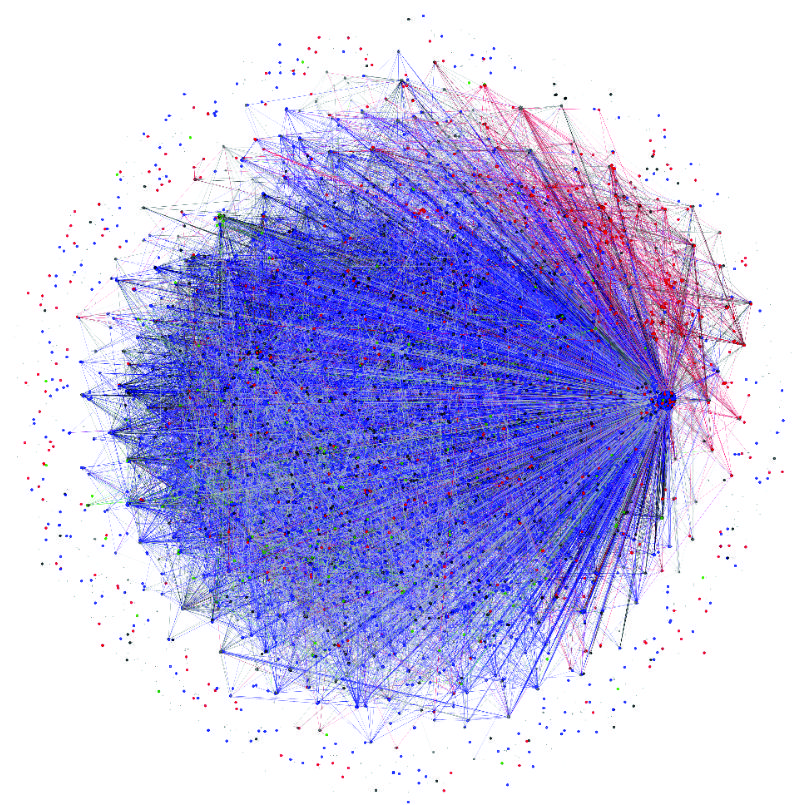
\includegraphics[width=0.419\linewidth]{openOrdGermany1}}
		\subcaptionbox{\label{fig:openOrdGermany-2}}{%
			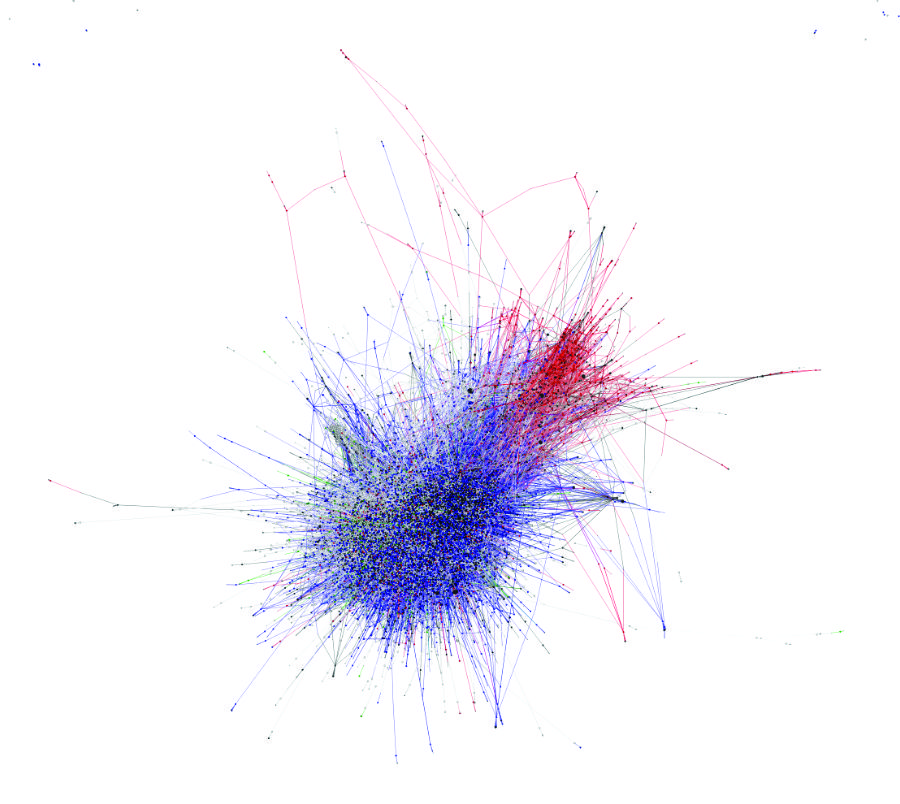
\includegraphics[width=0.4\linewidth]{openOrdGermany2}}
		\hfill
	}
	\legend{Blue: Cluster 1, ‘nationalists’; red: Cluster 2, ‘news disseminators’; green: Cluster 3, ‘anti-nationalists’; black: ‘overlappers’; grey: non-clustered users.}
	\caption{Communication within and between discursive groups of users in the discussions, with users as vertices and interactions (retweets and comments) as edges; reconstructed by OpenOrd and Force Atlas 2 algorithms for Germany.}\label{fig:openOrdGermany}
\end{figure}

\begin{figure}[ht]
	\centerfloat{
		\hfill
		\subcaptionbox[List-of-Figures entry]{\label{fig:openOrdUSA-1}}{%
			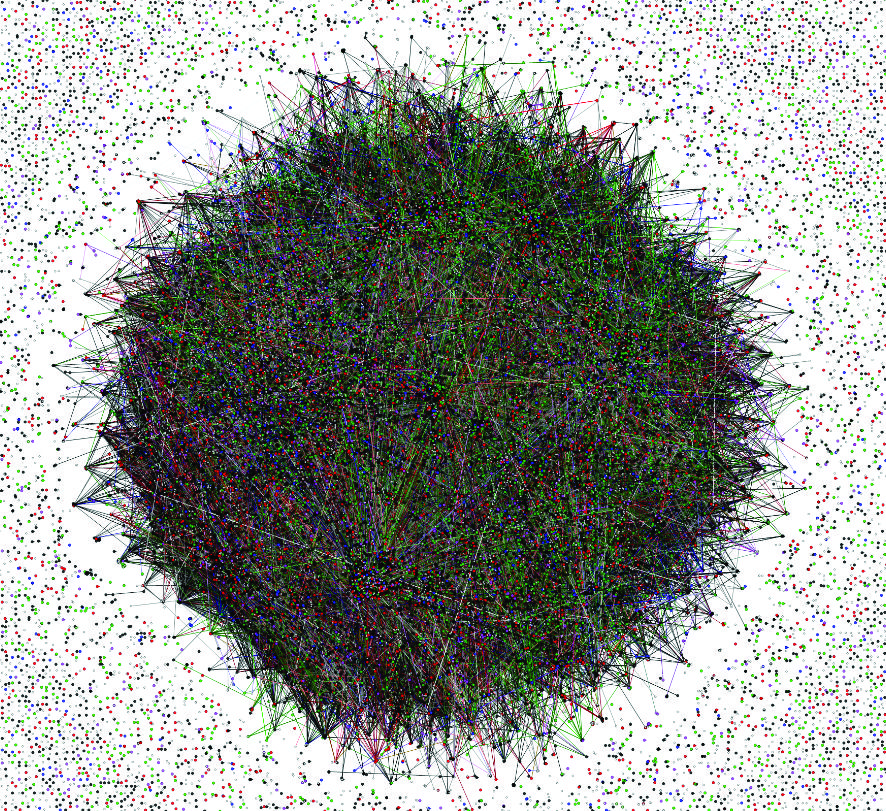
\includegraphics[width=0.419\linewidth]{openOrdUSA1}}
		\subcaptionbox{\label{fig:openOrdUSA-2}}{%
			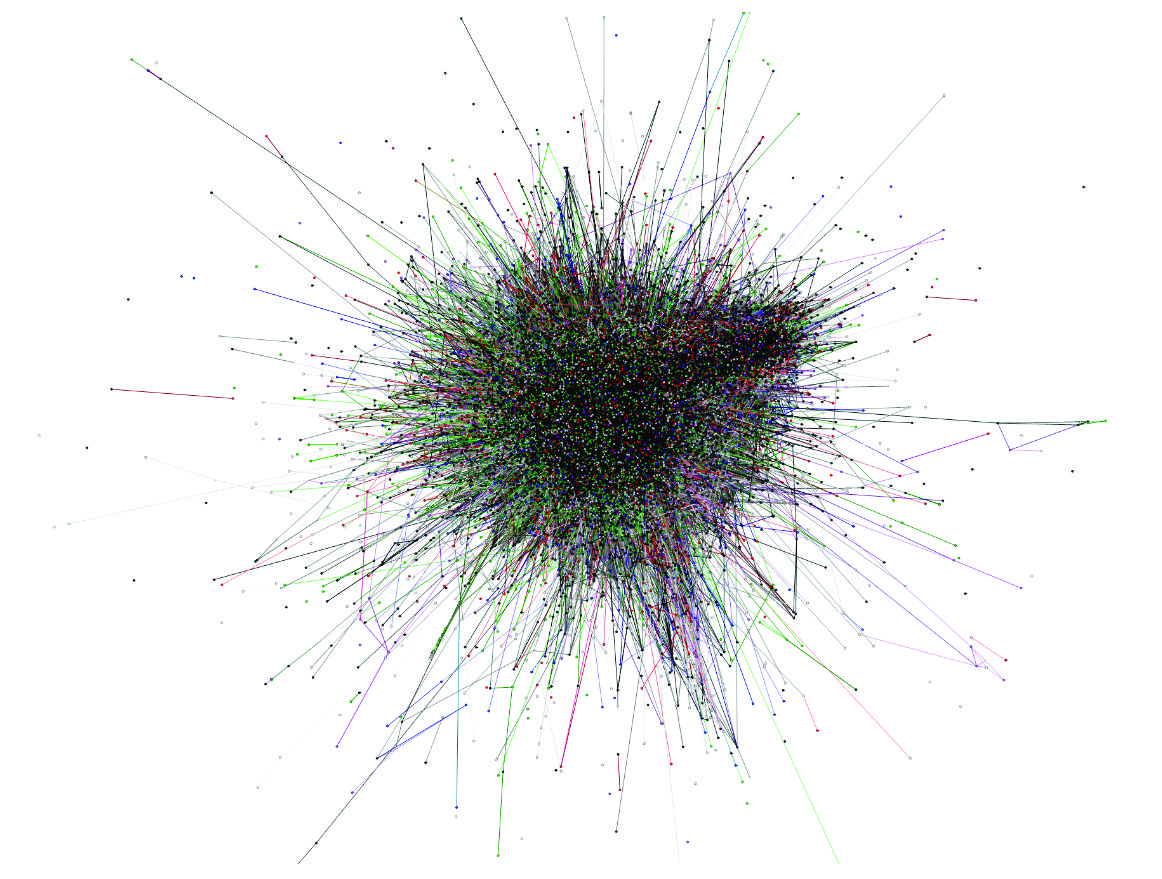
\includegraphics[width=0.4\linewidth]{openOrdUSA2}}
		\hfill
	}
	\legend{Blue: Cluster 1, ‘politicized observers’; red: Cluster 2, ‘media-oriented users’; green: Cluster 3, ‘human rights activists’; purple: Cluster 4, ‘whites’ blamers’; black: ‘overlappers’; grey: non-clustered users.}
	\caption{Communication within and between discursive groups of users in the discussions, with users as vertices and interactions (retweets and comments) as edges; reconstructed by OpenOrd and Force Atlas 2 algorithms for the USA.}\label{fig:openOrdUSA}
\end{figure}

To answer RQ2 about the left or right nature of the clusters, we partly recoded our coding data and corrected the graphs of means (Figures~\cref{fig:userAttitudesRussia} to~\cref{fig:userAttitudesUSA}) accordingly. Recoding was needed to re-interpret attitudes for and against a given actor as pro-left or pro-right. E.g., the influencers expressed attitudes towards political leaders (Obama, Merkel, and Putin), coded \(-2\) to 2. But, for the respective political spectra, Obama is leftist, while Merkel and Putin \cite{BluhmVarga} represent the rightist spectrum side. To ‘normalize’ the user attitudes, we recoded all the pro-left views as \(-1\) to \(-2\), and all pro-right views as 1 to 2 (see Table~\cref{tab:variableLeftRightNormalization}). By doing this, we could show on the graphs of means whether the clusters (and how many of them) were pro-left, pro-right, or mixed -- see Figures~\cref{fig:recordedDataRussia} to~\cref{fig:recordedDataUSA} for Russia, Germany, and the USA, respectively.

\begin{table}[ht]%
	\centering
	\caption{Recoding of variables for their left-right normalization.}%
	\label{tab:variableLeftRightNormalization}% label всегда желательно идти после caption
		\begin{adjustbox}{width=1\textwidth}
				\small
		\begin{tabular}{ c  c  c  c  c  c  c  c }% Вертикальные полосы не используются принципиально, как и лишние горизонтальные (допускается по ГОСТ 2.105 пункт 4.4.5) % @{} позволяет прижиматься к краям
			\toprule
			Country & Minority & President & Police-Authorities & Nationalists & Opposition & Democrats & Republicans\\
			\hline
			Russia & Recoded & Not & Not & Not & Recoded & -- & --\\
			Germany & Recoded & Not & Not & Not & -- & -- & -- \\
			USA & Recoded & Recoded & Not & Not & -- & Recoded & Not \\
			\bottomrule
		\end{tabular}%
			\end{adjustbox}
\end{table}

\begin{figure}[ht]
	\centerfloat{
		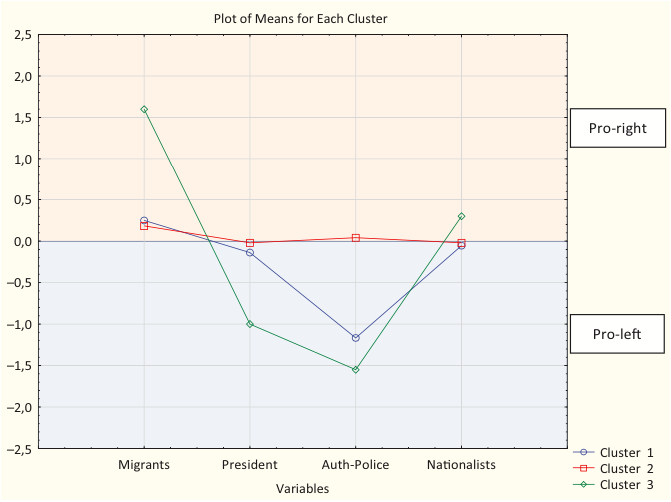
\includegraphics[scale=0.5]{recordedDataRussia}
	}
	\caption{Mean values for the recoded data on user attitudes towards the selected political actors for Russia.}\label{fig:recordedDataRussia}
\end{figure}

\begin{figure}[ht]
	\centerfloat{
		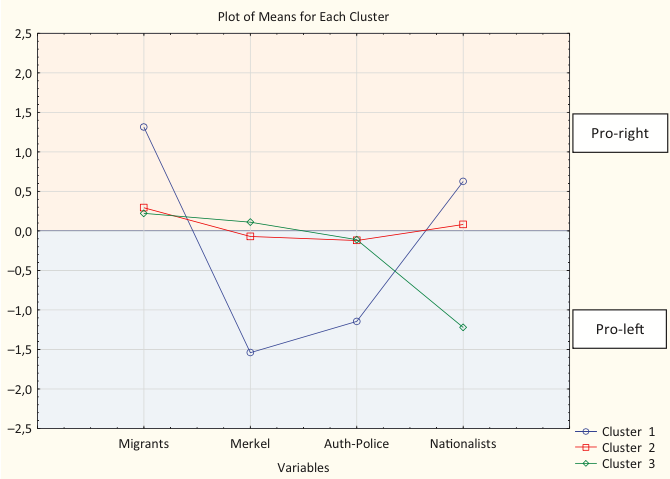
\includegraphics[scale=0.5]{recordedDataGermany}
	}
	\caption{Mean values for the recoded data on user attitudes towards the selected political actors for Germany.}\label{fig:recordedDataGermany}
\end{figure}

\begin{figure}[ht]
	\centerfloat{
		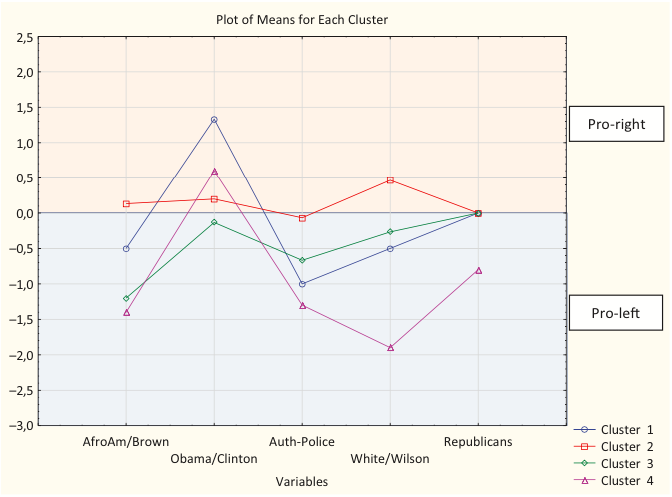
\includegraphics[scale=0.5]{recordedDataUSA}
	}
	\caption{Mean values for the recoded data on user attitudes towards the selected political actors for the USA.}\label{fig:recordedDataUSA}
\end{figure}

To answer RQ3, we qualitatively assessed the results for RQ1 and RQ2.

\subsubsection{4. Results}

Our results show that the discourses identified by coding influencers cover a substantial part of the discourse in all the cases: for Russia, the thesauri covered 31,5\%, in Germany, 63,4\% and, in the USA, 73,5\% of the users. This shows that influencers’ talk reflects the discourse of ‘ordinary users’ to different extents in each country, but everywhere we were able to detect the discourses that were important for the overall discussion.

As the figures suggest, in all the three cases, group structure was not binary; moreover, binary solutions for each country would hide important discourses that actually constituted the discussions. Neither did the group divisions correspond to the minority/pro-minority majority/anti-minority majority scheme. Instead, the clusters may be described as follows:

For Russia, the clusters include: ‘news disseminators’; ‘anti-establishment nationalists’; and ‘angry citizens’. The first group was mostly neutral but formed a substantial part of the political discussions by supplying (posting or retweeting) news at each stage of the conflict. The second cluster was clearly anti-immigrant and nationalistic but differed from European nationalism. Within the discussion, there was also an evident divide between the nationalist groups who supported the current establishment and those who actively opposed it. The former saw the incumbent leadership as the flesh of the 1990s’ elites who ‘had stolen the country’; such users, therefore, blamed the national policymakers for supporting the post-Soviet immigration. The second type of nationalism -- the pro-establishment one -- showed up in the third cluster of ‘angry citizens’. This cluster united anti-institutionalists who were raising voices against \textit{bespredel} (‘the absence of limits’ and rules of the game), but in differing ways. This diverse group included pro-Putin nationalists who were ready to fight with the Moscow riot police, liberal oppositional media and public figures who criticized the policymakers, and ‘tired citizens’ who negatively treated the immigrants, and the country leaders, and the local authorities, and the nationalists. Unlike in the ‘news disseminators’ cluster, the close-to-zero means for these variables here were the result of pro- and anti-establishment views compensating each other while the users united against police (see Figure~\cref{fig:userAttitudesRussia}).

For Germany, the clusters include: ‘news disseminators’; ‘nationalists’; and ‘anti-nationalists’. Discursively, the biggest group of ‘nationalists’ unites two similar sub-groups, one with slightly more aggressive tendencies towards small liberal-oriented parties and activist movements (like Antifa), and the other more critical of the national government. The anti-nationalist group is, however, also salient, making the German picture one-dimensional in terms of political divisions (pro- and anti-minority), even if the dimension is not political-party but issue-based. Also, the overlappers play a significant role here, as they visually stand in between the two opposing clusters, thus creating bridges for public dialogue (see Figure~\cref{fig:openOrdGermany}).

For the USA, the clusters include: ‘media-oriented users’; ‘human rights activists’; ‘politicized observers’; and ‘whites’ blamers’ (see Figure~\cref{fig:userAttitudesUSA}). Within the influencers, the clusters were similar in volume, but, on the big graph, the last two groups were relatively small- scale, while the first two dominated the graph. Just as in Russia, the media-oriented discourse was a part of the political discussion, but the three other groups were not neutral, especially ‘whites’ blamers’ and ‘human rights activists.’ The former actively blamed ‘the white dominance’ and called for action against oppression. Interestingly, the hashtag \#blacklivesmatter was less important for this group than for the media-oriented discourse. However, blaming hashtags and words like ‘murderer,’ ‘republikkklan,’ or ‘kkkop,’ and calls for action (like ‘\#arrestdarrenwilson,’ ‘\#boycottgofundme,’ or ‘\#donotshopmonday’), were prominent. The other group, very different from ‘whites’ haters,’ and linked the case to human rights issues like abortion (\#prolife), gender inequality (\#womeninequalityday), morality (\#moralmonday), and others. The group itself, as one can see even from the hashtags, was polar in itself in terms of left and right divisions on human rights. For this group, positioning on Mike Brown’s death was different, expressed mostly by ‘don’t shoot’ hashtags. ‘Politicized observers’ abstained from taking clear sides, but discussed the Ferguson events in terms of its influence upon the political process in America. Interestingly, the cluster that mostly reposted media, was the most pro-Wilson, as media, evidently, tried to remain balanced; they also reported police press conferences that were modestly defensive towards Darren Wilson.

Then, we looked at how the discourses we described spread inside the graph. Our task was not to calculate the level of homophily and prove user clustering for all the discussions; the goal was to see how the discourses actually spread and whether they spread in a similar way -- and they did not. For Russia and the USA, the discourses mixed, but if in Russia we saw inter-cluster talk, in the USA overlappers took almost all the space in the graph centre. And in Germany, the graph was clearly structurally divided. This was also proved by the mean in- and inter-cluster weighted number of edges: in Russia, the inter-cluster links took over (216 vs. 323.5, respectively), while in Germany (4392.75 vs. 2890.25) and the USA (21114.4 vs. 3755.2) in-group connections were stronger.

Thus, the attitude-based grouping was different in each of the three cases. Also, it was far from clear left-right identifications. In order to show it, we have recoded the variables as stated above, making pro- left views negative (\(-1\) to \(-2\)) and pro-right views positive (1 to 2). We considered anti-minority, anti-Obama/Clinton, pro-Putin/Medvedev, pro-Merkel, pro-police, pro-nationalist, anti-opposition (in Russia), anti-Democrat, and pro-Republican (in the USA) views pro-right, while the opposite was marked pro-left. See the full recoding scheme in Table~\cref{tab:variableLeftRightNormalization}.

The resulting graphs of means are quite telling (see Figures~\cref{fig:recordedDataRussia} to~\cref{fig:recordedDataUSA}). Both in Russia and Germany, the leaders representing rightist sides of the spectra have actually taken pro-migration stance, and this has made right-wing users who support nationalist movements and speak against immigrants, move left and be against the incumbent leaders, as well as against the local authorities and police for ‘not protecting’ the host communities. But the other clusters in the two countries quite strongly differ from each other. While in Germany issue-based leftism is clearly seen, the other Russian cluster of ‘angry citizens’ diverges into three discourses that combine clearly rightist, pro-establishment nationalism; liberal, anti-establishment oppositional speakers; and politicised citizens. These politicised citizens, paradoxically for external observers, do not support any of the existing political factions, due to their impotence in resolving local problems. Thus, at least two nationalist discourses were detected by us for Russia -- while in the USA there are two very different left-wing clusters, one clearly left, supportive of either Obama or Clinton and based on human rights’ discourse, and another that was sharply anti-white, even blaming Obama for not being protective enough, which, in our rough coding, made the cluster stick out to anti-Obama views on the rightist side of Figure~\cref{fig:recordedDataUSA} (in effect, being extreme left). The cluster of ‘politicized observers’, interestingly, is reminiscent of the ‘tired citizens’ in Russia, as they are, on average, only slightly pro-African-American and, more strongly, anti- leader, anti-police, and anti-majority.

Another crucial observation is that, while the divisions in the discussion clearly stem from local political contexts, they are quite far from expectations determined by the systemic political features of the countries. Thus, in the majoritarian USA where one would expect two-sided polarization, the clusters were, in fact, numerous and the discussion was based on overlappers. It was rather coalitional Germany that showed polarization. And in Russia, just one side of the spectrum was present in the discussion. Thus, it is not only the local political markets but also the nature of the issue and issue-based divisions that shape political clustering
.
Overall conclusions are thus the following: The discursive schisms do exist in issue-based discussions, but they do not fall into binary categories according to majoritarian political divisions, and; they only partially fall into the three-side divisions expected by the nature of the issue. Instead, local political spectra may provoke the formation of, for example, two leftist or two rightist clusters. Only Germany has demonstrated the expected divisions between anti- and pro-minority majority, while the minority remained highly under-represented at all, like in Russia -- and unlike in America.

The similarities can also be traced, but not in terms of left and right divisions. First, in all the discussions, a politically neutral news-based cluster played a significant structural role. Second, all three discussions revealed harsh anti-institutionalism, including that from the users who, in conventional logic, were expected to support the incumbents. Third, Germany and Russia were similar in how nationalist clusters were against the conservative governments, and Russia and the USA were similar in how the ‘tired citizens’ were politicised against all the political sides.

\subsubsection{5. Conclusion}

In our article, we have combined content analysis of social media with cluster analysis and graph construction. Our method has revealed greater complexity of politicised discourse within ad hoc Twitter discussions on inter-ethnic conflicts. Thus, we have found that there may be several clusters of leftist or rightist views even if the number of clusters is minimal, and users may combine formally leftist and rightist views if positions of political actors or the nature of the issue demand it. The groups we have detected differ highly in their conceptualisation from the traditional left and right divisions and left or right labels cannot be attached to individual users based on their preferences, like pro- and anti-minority stances or treatments of country leaders or parties. We have also shown that, on the graphs, the discourses intertwine quite intensely if we do not force the graphs to artificially diverge according to users’ political views.

Our research provides new input for rethinking the political divisions that form online, on what grounds they form, and how to detect them. The local political contexts, as well as the nature of the issues under scrutiny, are major factors to be taken into account. In our article, the ‘issue publics’ provide clues on how political opinion is veering away from traditional left and right divisions, and Twitter communication is more complicated than the imaginary cocooned talk in echo chambers, especially for issues beyond elections and direct policing.

Limitations of our method stem from the subjectivity of coding and from the low number of coded influencers, but these may be partially overcome by automatisation of coding collections and the increase of the number of coded users thanks to automatisation. Our method may be applied to detect hidden issue-oriented polarization beyond one-dimensional left-right political spectra.

\subsection{Please Follow Us: Media roles in Twitter discussions in the United States, Germany, France, and Russia}\label{subsec:ch5/sec1/sub2}

\subsubsection{Introduction}

The evolution of online journalism in the past decades has triggered the transformation of traditional journalism conceptions, challenging some core principles of journalism, such as the gatekeeper role and objectivity \cite{SchudsonAnderson} and blurring the boundaries of the profession \cite{Franklin}. A rich body of research has explored the shift in journalism role perceptions \cite{SchudsonAnderson,Hermida,Waisbord,WeaverWillnat} as well as in journalism practices and performance \cite{Pavlik,LasorsaLewisHolton,Vis}. There is an understanding that technologies shape journalism practices \cite{Pavlik,Mellado}; however, it contests whether the use of digital platforms has led to a change in the core values of journalism. Some scholars have assumed that the major norms of journalism and journalistic roles still endure \cite{Fenton,Waisbord,AlRawi}, while others have concluded that old norms are being transformed by new practices \cite{Gillmor,Reese,LindnerConnellMeyer}.

Cross-national comparisons provide evidence that these processes may differ in various socio-political contexts \cite{HallinMancini2012}. However, most of the studies explore Western contexts \cite{EngesserHumprecht,LarssonKalsnesChristensen}. There are several that have recently gone beyond Euroatlantics \cite{AkohAhiabenu,AlRawi,SaldanaHigginsJoyceSchmitzWeiss}, but they still selected the countries based on their regional proximity. By contrast, our study looks at the role performance of different types of legacy media on Twitter, both in and beyond the Western world.

Our approach combines the assessment of role performance as based on the content of tweets by the media and journalists with an estimation of the positions of media/journalist accounts in the discussion network. Thus, we argue, we are able to link the role-based practices of the media/journalists to their resulting positions within online discussions.

To answer our research questions, we look at recent inter-ethnic conflicts in the United States, Europe, and Russia; these conflicts were all triggered by violence, provoked social polarization and massive public discussions, heavily involved authorities and local communities, and had policy implications. Despite different scales of global reach, they all made it into the national trending Twitter topics and today remain the reference points for public discussions on inter-ethnic relations in the respective countries. For such conflicts, it is crucial to know whether media fulfill the roles of bridging the discussion echo chambers, providing information, and organizing discussion zones within Twitter.

The remainder of the paper is organized as follows. First, we review the literature on journalism roles in the digital age, with special attention given to media performance on Twitter and to the technical ways of defining key users in the discussion. Then, we present the hypotheses and methods of our research, followed by findings and discussion. Drawing on the results of our analysis, we propose our typology of media roles in Twitter discussions.

\subsubsection{Research Premises}

\paragraph{Journalistic Roles in the Digital Age}

The classification of journalistic role models began in the 1960s, with the dichotomist typology introduced first by Cohen \cite{Cohen} and then by Johnstone, Slawski, and Bowman \cite{JohnstoneSlawskiBowman}, wherein reporters were described as neutral observers or participants. A similar approach was also used by Weaver and Wilhoit \cite{WeaverWilhoit,WeaverWilhoit1996} in their survey of US journalists. They added one more role type to the earlier classification, labeling the roles as “disseminator,” “interpreter,” and “adversarial.”

In the twenty-first century, McNair proposed three role models according to the roles of journalists in the democratic process: watchdog/fourth estate, mediator/representative, participant/advocate \cite{McNair}. Hanitzsch \cite{Hanitzsch} explored the cultural backgrounds of journalists to develop his typology of role models, which he applied to the cross-country study of journalism cultures \cite{HanitzschHanuschMellado}. Mellado \cite{Mellado} developed her typology based on factors such as the relationship of journalism with elites, the level of subjectivity in the content, and journalist–audience relations, defining disseminator–interventionist, loyal, watchdog, civic, service, and infotainment role models (see also \cite{MelladoLagos}).

Obviously, not all of these typologies can be operationalized to compare journalism roles across democratic and non-democratic contexts. Also, most of them are aimed at studying the role concepts as articulated by journalists, whereas our study aims to analyze the role performance based on content analysis and on the resulting positions of media and journalists in the discussion structure. Therefore, in our study of journalism role performance on Twitter, we have set sail from the earlier typology based on how journalists construct their content: (1) disseminators (convey facts) and (2) interpreters (convey not only facts but also opinions). Then, we have combined this knowledge with the pos- itions of the media in the discussion web graphs and user top lists. The resulting roles that we have formulated trace this “performance-position” axis. We have left out the role perception aspect, as this lies beyond our scope.

Cross-national comparisons of professional journalism have shown the prevalence of some role models in certain countries \cite{Donsbach,HanitzschHanuschMellado,Waisbord} and journalistic role perception being influenced by the type of media system \cite{WillnatWeaverChoi}. Thus, advocacy journalism has been historically more popular in Western Europe compared to the United States \cite{Waisbord} and in Eastern Europe compared to Western Europe. A survey of political journalists in Denmark, Germany, the United Kingdom, and Spain \cite{VanDalenDeVreeseAlbaek} revealed that Spanish journalists were more partisan in delivering news than their colleagues in other countries. The comparison of the perception of journalism functions in Germany and Russia has also shown crucial differences: in Russia, journalists often perceive themselves as “educators” of the audience, and opinionated journalism is more popular compared to Germany \cite{Litvinenko}. Comparison of professional journalistic cultures in Poland, Russia, and Sweden \cite{NygrenDobekOstrowska} supports the view of Russia as a country with more blurred boundaries between impartial journalism and media advocacy practices.

Drawing on these studies, we would assume that, in our sample, the Western media would look more like information disseminators compared to the Russian media. Among the Western cases, the US legacy media should, in theory, be more restrained from expressing opinions than French and German media outlets.

Apart from the macro-level factors such as socio-political context, media scholars have also focused on exploring organizational factors that shape role performance. The same technologies are being adopted in different ways depending on organizational factors within newsrooms \cite{Boczkowski,Domingo,PaulussenUgille}, “routine influences and organizational location [being] stronger and more consistent predictors of role enactments” than the role conceptions articulated by journalists \cite[p.~550]{TandocHellmuellerVos}.

Lasorsa, Lewis, and Holton \cite{LasorsaLewisHolton}, in their study of journalists’ performance on Twitter, have found that the “elite” media stick more to their role of “neutral observers” compared to other outlets. Another difference in role performance may arise from the insti- tutional status of the Twitter accounts -- that is, media accounts would differ from those of individual journalists, and the latter also have different degrees of openness in sharing their opinions, depending on their personal branding strategies \cite{LasorsaLewisHolton}. In our study, we have explored whether these patterns also work across national contexts.

\paragraph{Journalistic Roles on Twitter: Platform Dependence or New Flexibility?}

Since the launch of Twitter in 2006, a large body of academic research has emerged studying different aspects of its impact on journalism, with two major research strands exploring (1) how media and journalists use the affordances of the platform in their work \cite{BroersmaGraham2013,MelladoVanDalen,PaulussenHarder,Hedman,WeaverWillnat,TandocVos} and (2) how the use of Twitter transforms the core norms of journalism \cite{BrunsHighfield2012,HayesSingerCeppos,Hermida,SkogerboKrumsvik}.

It seems that the Twitter strategies of media accounts so far have formed a smaller research field than the Twitter practices of individual journalists. For institutionalized media accounts, previous research shows that, in their online behavior, the media tend to preserve the pre-Twitter communicative hierarchies, where they played the role of key nodes in information flows and participated in top-down information dissemination (for a review, see \cite{BodrunovaLitvinenkoBlekanov2016}). Thus, the media are usually retweeted by more users than on average and gain authority, but are still “far and away the most followed” and are the least active in retweeting or commenting on other users -- except for their fellow journalists \cite{LotanGraeffAnanny,GroshekTandoc}. Some works have also demonstrated that the importance of media accounts in shaping the discussion structure and dynamics is exaggerated, as “only a small portion of tweets received by ordinary users come from media outlets” \cite[p.~269]{BastosRaimundoTravitzki}. However, the media still remain highly relevant for Twitter users in times of crises or natural disasters \cite{Vis,Bruns2014}; thus, we expect them to be among the high-ranking users.

As for journalists, studies of their role models on Twitter usually show the tendency of journalists to “normalize” their practices, so that they fit into the existing traditional role models \cite{LasorsaLewisHolton,TandocVos}. Early research on the political blogosphere \cite{Singer2005} has shown that journalists prefer to perform their traditional roles as gatekeepers while working with Web 2.0 platforms. Comparison of Arabic and English news organizations on Twitter revealed that the editors followed the same news values as on other media channels \cite{AlRawi}. However, most studies also show that the affordances of Twitter force journalists to adjust their existing norms and “re-invent” journalistic identity to a certain degree \cite{Olausson}, as journalists “frequently experience confusion between their roles as reporters, editors, critics, or independent individuals” and, as a consequence, “use Twitter in a way that supplements their traditional role as information disseminators” \cite[p.~267]{PapacharissiDeFatimaOliveira}. Lasorsa, Lewis, and Holton \cite{LasorsaLewisHolton} built their study on the research by Singer \cite{Singer2005}, exploring how the platform challenges the existing norms of journalists, making them, inter alia, deviate from their role as nonpartisan information providers by expressing personal opinions, which contests the journalistic norm of objectivity \cite{LasorsaLewisHolton}. The authors also spotted different strategies of conduct of journalists on Twitter, depending on the status of their media outlets: the local editors were more willing to share their personal opinion than journalists from the nationwide elite media \cite{LasorsaLewisHolton}. Our study scrutinizes this aspect of deviation from the traditional norms (a tendency of more opinionated journalistic content on Web 2.0) suggested by Singer and explored on Twitter by Lasorsa and colleagues, and expands the analysis to a cross-national level.

\paragraph{Journalists as Influencers: Technical Ways to Assess User Roles in Online Discussions}
As stated above, assessment of the discursive performance of the media/journalists has been predominantly based on a normative understanding of journalistic roles in society and content analysis that corresponds with this understanding to varying extents. However, previously, scholars have rarely been able to link role performance to the actual place of media within open discussions.

Today, social network analysis (SNA) allows for the structural representation of the roles of users within discussions on social media platforms. With understandable limitations that come from the fact that the dynamics of the discussion is presented statically, SNA-based research on social media provides ways to link the user position within the network, or the so-called \textit{influencer} status \cite{PattersonGrennyMaxfield}, to other user-related factors, such as the nature of the account, user behavior, content of tweets, or his/her offline status. For this paper, we have tried to link a content-based assessment of media roles to the positions of the media within the discussion networks, which would allow for assessment of not only the normative performance but also the resulting position -- and, later, tracing whether observer or interpreter roles lead to greater influence within a discussion. So far, such research has been scarce (see \cite{EnliSimonsen}).

As we have shown elsewhere \cite{BodrunovaLitvinenkoBlekanov2016,BodrunovaLitvinenkoBlekanov2017}, two approaches for measuring user influencer status may be seen in today’s literature; the difference has been conceptualized as “activity metrics versus connectivity metrics.” Thus, the first approach relies on user activity metrics expressed in absolute figures, such as the number of tweets, likes, retweets, and comments, as well as on the number of followers. Among these metrics, the latter is less relevant for ad hoc discussions due to their short-term nature. Regarding other metrics, retweets are considered, in the vast majority of literature, to be the most adequate metric for detecting influencers \cite{FrebergGrahamMcGaughey,BrunsBurgess2015,SajuriaVanHeerdeHudsonHudson} (see also earlier works by boyd, Golder, and Lotan \cite{BoydGolderLotan}; Cha et al. \cite{ChaBenevenutoHaddadi}). Nonetheless, there are also works that demonstrate the importance of comments and measures combining likes, retweets, and comments \cite{Vis}; thus, we have used them all and checked whether media enter the top user lists by these metrics.

Another line of research relies on SNA-based metrics such as various types of graph centralities \cite{ChaBenevenutoHaddadi,DuboisGaffney}, as well as their combinations \cite{GonzalezBailonBorgeHolthoeferMoreno} and author-specific derivatives \cite{MairederWeeksDeZuniga}. This approach differs from the first due to the fact that some SNA metrics are network-dependent -- that is, the position of a given user in the user ranking by this metric is relative and depends on the overall shape of the network. Thus, these metrics tend to be more discussion-specific, while the authority measured by absolute metrics (such as the number of followers) may be inherited by the users from the pre-discussion period.

For this research, we have assessed positions of the media/journalists in top user lists by several SNA metrics. These metrics would be indegree, outdegree, degree, betweenness, and pagerank centralities. The first three assess the number of individual users who have interacted with a given account (indegree), with whom the given account has interacted (outdegree), and their sum (degree), which shows the level of user involvement in the discussion. These metrics are not identical to the number of likes, retweets, or comments, as one user may “like” or comment on tweets by another user many times, but the connection will still count as 1. Betweenness centrality, in its essence, shows the capacity of a user to be a shortcut between other users and user groups. Pagerank centrality shows how authoritative a given user is among other authoritative users. In our view, these metrics allow for assessment of the structural position of a user with enough precision.

However, it may happen that a user is ranked high by several metrics, so this needed to be assessed separately. For this, we have used reconstructed web graphs that show top users for whom the network metrics were combined.

\paragraph{Research Questions and Hypotheses}
Having in mind everything stated above, we have formulated the following research questions:

\paragraph{RQ1. How do the roles of the media/journalists in the conflict discussions on Twitter differ based on the institutional status of the tweeter (the media/journalist), the online/offline nature of the media, and the media format and reach?}

\paragraph{RQ2. Do these differences repeat across countries? Or, do they differ the way the respective media systems do?}

\paragraph{RQ3. Do the media play important roles in the discussion structure across cultures? How can we re-conceptualize the media/journalist roles based on their place in the discussion?}

To answer RQ1 and RQ2, we have stated the following hypotheses:
\begin{itemize}
	\item H1. In all four cases, due to the nature of Twitter as a platform, the media will tend to perform the roles of information disseminators more than those of interpreters/opinion propagators.
	\item H2. Of all the media, large-scale quality media (that is, national news and public affairs outlets) will adhere to the information disseminator role, unlike other types of media and individual journalists.
	\item H3. However, in Russia, legacy media will have more opinionated content compared to Western countries, and, in France and in Germany, more than that in the United States.
\end{itemize}

For RQ3, we suggest the role descriptions based on the assessment of the content of tweets, the aforementioned user metrics for top users, and the visual positions of influential media and journalists in the discussion graphs. We have evaluated the graphs qualitatively to see whether media of the same type tend to be in similar graph positions.

\subsubsection{Methodology, the Research Process, and the Cases Under Scrutiny}

\paragraph{The Cases Under Scrutiny}
The cases selected for comparative analysis had six features in common, as they all: (1) had a violent trigger; (2) caused outstanding public discussions (reaching national and sometimes global Twitter trending topics) and significant social polarization; (3) were related to inter-ethnic/inter-race tensions; (4) caused street action; (5) demanded intense involvement of local and national authorities; (6) had policy consequences in terms of public security and/or migration. These features allow us to say that these cases, despite their differing scales of international coverage, are comparable within national contexts. Thus, the cases included:
\begin{itemize}
	\item Clashes between local dwellers and immigrants from Central Asia in the Moscow district of Biryulevo, Russia, September 2013. After an alleged killing of Muscovite Egor Scherbakov by Uzbek immigrant Orkhan Zeinalov, the population of the Biryulevo district has ruined the local warehouse where hundreds of immigrants dwelled and traded (many of them illegally). Several peaceful “people’s gatherings” followed.
	
	\item Anti-police riots in Ferguson, Missouri, United States, August 2014. After white police officer Darren Wilson killed an unarmed African American teenager named Mike Brown, the town of Ferguson, as well as other places across America, exploded with street protests and peaceful support actions.
	
	\item An attack on Charlie Hebdo in Paris, France, January 2015. Attackers killed 10 journal- ists and cartoonists from the French magazine and more people in Paris and beyond. Massive peaceful support actions followed in France and around the world; the public split under the hashtags \#JeSuisCharlie and \#JeNeSuisPasCharlie.
	
	\item Mass public harassment of females on New Year’s Eve in Cologne, Germany, January 2016. During the celebrations, over 1000 (self-reportedly) were harassed, mostly by men of North African and Middle Eastern origin. Protest actions followed, as well as intense discussions on social media, while national legacy media remained silent for several days.
\end{itemize}

\paragraph{Research Methodology and the Research Process}
Overall, our methodology is comprised of vocabulary-based Web crawling within Twitter (“Twitter crawling”), discussion graph reconstruction, formation of top user lists based on the aforementioned user metrics, manual selection of media and journalists’ accounts from top user lists, automated sampling of their tweets from the corpora of the tweets uploaded, manual coding of content from the tweet datasets, assessment of the saliency of opinionated content, and qualitative clustering of the media/journalists based on the saliency of opinionated content as well as on the media’s type and reach.

Our pre-tests included comparison of our uploads to standard application programming interface- (API) based ones, as well as dealing with the ad hoc nature of the discussions. Previous literature raised the problem of the non-comparability and low predictability of \textit{ad hoc} discussions formed by “affective” and unstable “issue publics” \cite{BrunsBurgess2015,Papacharissi}; we argue that the discussions are more comparable in their structural nature than was thought before, though the results have not yet been fully reported.

Then, the research steps were the following:
\begin{enumerate}
	\item For each case, hashtags and keywords were selected on trendinalia.com; for Russia and Germany, “snowballing” reading of over 1000 tweets helped to define additional keywords.
	
	\item We conducted Twitter crawling based on the selected keywords. For this, we used a specially developed Web crawler with adaptable modules \cite{BlekanovSergeevMartynenko}. Our crawler uses a collection technique similar to manual collection, and thus minimizes the well-known API limitations, such as limits on GET-requests, the impossibility of defining the IDs of commenters and retweeters, limitations on historical data, and distortions due the changing “tweet popularity” algorithm. The crawling procedure included two steps: (1) collecting all the publicly available tweets with the pre-defined keywords and (2) collecting likes, comments, and retweets for these tweets, for us to be able to reconstruct the discussion graph. No exclusions were made within the automated procedure; irrelevant tweets were eliminated from tweet collections later on (see Step 7).
	
	\item Then, we reconstructed the discussion graphs and analyzed the user metrics, both absolute and relative. The resulting directed graphs had users as nodes and their interactions (likes, comments, and retweets) as edges. N tweets posted affected the size of the node; N interactions affected the visual closeness of users to each other. The visual representations of the graphs, however, were non-directed, for the sake of clarity; despite the fact that this has made the representation of directions of the communication flows in the graphs impossible, we have preferred to focus on the dis-cussion structure and key users.
	
	\item We formed lists of the top 100 users via nine metrics (\(N\) tweets, likes, retweets, and comments; indegree, outdegree, degree, betweenness, and pagerank centralities); thus, we received lists containing altogether 3600 mentions of Twitter accounts. The real number of the accounts for each case was, of course, lower, as some of the accounts were found in more than one top list. We established the threshold of the top 100 users per metric not only because of its feasibility, but also in accordance with our previous research \cite{BodrunovaLitvinenkoBlekanov2016,BodrunovaLitvinenkoBlekanov2017}, where we have seen that, within 100 users, there are quite a lot of those who are in the top lists by many parameters; below 100 top users, the divergence of the lists grew.
	
	\item Wemanuallycheckedthe3600accountmentionstofindthemediaandjournalists. All the media accounts, as well as those of journalists, were double-checked outside Twitter. Only journalists from established media outlets (licensed newspapers and registered audiovisual and online-only media) were taken into account; no freelance commentators, bloggers, or individual Web portal creators were included; media-like Twitter accounts were also outside our scope. We also drew the line between foreign and domestic media, which was not always easy. Thus, local media in languages other than the “title” language of the case (like \textit{The Moscow News}), as well as state-supported “overseas broadcasting” companies (\textit{Deutsche Welle}, \textit{RT (Russia Today)}), were considered foreign and were not included in the samples for coding, while franchise outlets in local languages (like \textit{LeHuffPost} or \textit{Forbes Russia}) were included in the samples. We included (mostly from the United States) several accounts of online-only media that had grown out of user-generated content (like \textit{The Huffington Post}, \textit{Mediaite}, or \textit{Mashable}), as they had gained a significant position in the respective media markets, and excluding them would have distorted the real picture of the discussions.
	
	\item We extracted all tweets by media and journalists from the uploaded tweet collections and formed four datasets for manual coding.
	
	\item We coded all the media tweets with the help of experienced coders. The coding followed a simple scheme: 0 -- information tweet or full quote; 1 -- opinionated tweet (opinion, rhetoric question, emotional claim, call for action, commented quote); 99 -- irrelevant tweet (spam, tweets in other languages/of irrelevant topics/containing hashtags only, and same-day full replicas -- that is, tweets that fully replicated other tweets posted by the same user the same day, which is one of the indications of bot activity). Two coders for each country (one media expert and one native speaker) performed the coding; their interrater reliability was checked in pre-code tests and was over 0.68 (Cohen’s kappa) in each case. The main coder was the media expert; native speakers were involved for random double-checks and coding of controversial cases.
	
	\item We clustered the accounts according to: (1) their type (hybrid/online-only/journalist),
	reach (national/other for hybrid media) and format (quality/other for hybrid media), and (2) the percentage of opinionated tweets in their content. We understand those under hybrid media to have both online and offline versions \cite{Chadwick} and to have started offline. To distinguish quality media from tabloid and enter- tainment media, we used the definition by \cite[p.~71]{Norris} as based on physical format, style of writing, subject matter of the content (including what is considered news for a given media outlet), and orientation with potential political impact (or its absence).
	
	\item Wehavevisualizedthediscussiongraphintwoforms:(1)thefullgraphsand(2)the users from the top lists, to see where media of various types and reaches stood within the discussions. We highlighted local media, journalists, and foreign media among top users and qualitatively assessed their place in the discussion graphs.
	
	\item We described the roles of the media/journalists based on the saliency of opinionated content and the place of the media/journalists in the top lists and the graphs.
\end{enumerate}

\paragraph{Sampling and its Limitations}

Due to differing scales of coverage of the cases in both legacy and social media, we had to be flexible with our sampling strategy. Moreover, the apparatus limitations came into play when we encountered the volume of uploads for the US and French cases. The third consideration was that the cases were different in their pace, and thus the upload periods would differ as well.

Therefore, we uploaded the content from two weeks of the discussion for Russia and Germany, one week for the United States, and only three days for France. The biggest limitations that we experienced were with Ferguson; in 2014, we were still unable to upload the first week of the discussion due to its volume, and we focused on the second week, with Mike Brown’s funeral as the central event. As later research revealed, we were right in our selection, as Week 2 showed only a slight decline in the presence of both hybrid and online-only media entities in the discussion of Ferguson \cite{GroshekTandoc}. The three-day limitation for France is explained by the necessity of making the datasets comparable and feasible for coding. Thus, our initial sampling resulted in 901 tweets for Russia, 1010 tweets for the United States, 1692 tweets for Germany, and as many as 4739 tweets for France.

Another point of discussion for sampling was the media and journalists included in the samples. Our strategy was to include only the media that openly claimed to be such, including legacy media and online-only media that focused on current affairs and public agendas; niche media (sports, music, etc.) were excluded, as well as activist media sites, blogs, Twitter-only news streams, bots, and news aggregators. Also, in each case, we excluded international media and national media working in other languages; thus, RT in Russian was included for Russia, but RT in English was excluded for Russia, the United States, and France. Regarding journalists, we excluded foreign journalists, as well as bloggers, freelance journalists with no stated affiliation, and journalists with undetectable work affiliation. Thus, we formed the datasets of national legacy (offline and online-only) media and their journalists.

Then, after formation of the full lists of media, we excluded from the analysis the media that had posted fewer than four tweets, as calculating percentages for their tweets would create large distortions in the overall picture. Thus, the results that we are presenting only include the media and journalists who posted four tweets or more. After eliminating low-activity accounts and tweets coded 99, the datasets included the number of users and tweets shown in Table~\cref{tab:finalDatasets}.

\begin{table} [htbp]%
	\centering
	\caption{The final datasets.}%
	\label{tab:finalDatasets}% label всегда желательно идти после caption
	\renewcommand{\arraystretch}{1.5}%% Увеличение расстояния между рядами, для улучшения восприятия.
	\begin{SingleSpace}
		\begin{tabulary}{\textwidth}{@{}>{\zz}L >{\zz}R >{\zz}R >{\zz}R >{\zz}R@{}} %Вертикальные полосы не используются принципиально, как и лишние горизонтальные (допускается по ГОСТ 2.105 пункт 4.4.5) % @{} позволяет прижиматься к краям
			\toprule     %%% верхняя линейка
			& Russia & United States & Germany & France \\
			\midrule %%% тонкий разделитель. Отделяет названия столбцов. Обязателен по ГОСТ 2.105 пункт 4.4.5
			Total users & 29 & 14 & 48 & 47 \\
			Media & 26 & 11 & 32 & 37 \\
			Journalists & 3 & 3 & 16 & 10 \\
			Total tweets & 805 & 558 & 1512 & 3277 \\
			Tweets by media & 785 & 408 & 1149 & 2808 \\
			Tweets by journalists & 20 & 150 & 363 & 469 \\
			\bottomrule %%% нижняя линейка
		\end{tabulary}%
	\end{SingleSpace}
\end{table}

\subsubsection{Results}

\paragraph{Testing the Research Hypotheses}
\textit{H1.} To assess the saliency of opinionated content in various types of media, we have conducted content analysis of the tweet datasets from Table~\cref{tab:finalDatasets}. The resulting distributions of media/journalists’ accounts by type and reach are shown in Table~\cref{tab:opinionatedContentSaliency}.

\begin{table}[ht]%
	\centering
	\caption{Saliency of opinionated content in media accounts.}%
	\label{tab:opinionatedContentSaliency}% label всегда желательно идти после caption
	\begin{adjustbox}{width=1\textwidth}
		\small
		\begin{tabular}{ l  l  l  l  l  l }% Вертикальные полосы не используются принципиально, как и лишние горизонтальные (допускается по ГОСТ 2.105 пункт 4.4.5) % @{} позволяет прижиматься к краям
			\toprule
			\multicolumn{6}{c}{\makecell{Hybrid}}\\
			\cline{2-4}
			Percentage of opinion tweets & National quality/public service & National other & Regional & Online-only & Journalists \\
			\hline
			Russia&&&&&\\
			
			Under 10 & \makecell[l]{\textit{Kommersant}\\Silver Rain radio\\Voice of Russia\\RT Russian\\Public Service TV} & \makecell[l]{\textit{Lifenews}\\\textit{Izvestia}\\\textit{Krugozor}\\Mir24\\NTV\\\textit{Sovershenno Sekretno}} & \makecell[l]{\textit{The Moscow News}\\Federal Press}&\makecell[l]{\textit{Foxtime.ru}\\\textit{Okno v Rossiyu}\\\textit{Pravde v glaza}} & A. Poltoranin\\
			
			11--30 & \makecell[l]{RBC\\TV Rain} & \makecell[l]{\textit{Metro}\\\textit{Komsomolskaya Pravda}\\REN TV\\REN TV News} & &National News Service & \\
			
			31--50 & \textit{Novaya gazeta} & & & \textit{Grani.ru} & V. Zlobin\\
			
			51 and over & & & & \textit{Pravda.ru} & A. Kotz\\
			
			United States&&&&&\\
			
			Under 10 & Fox 2 News St. Louis & & & & \makecell[l]{R. Reilly\\L. Brown}\\
			
			11--30 & \makecell[l]{MSNBC\\\textit{The Washington Times}} & & STL Public Radio & \makecell[l]{\textit{Mashable}\\\textit{Mediaite}} & \\
			
			31--50 & & & St. Louis on the air & \textit{HuffPost Politics} & \\
			
			51 and over & \textit{Newsweek} & \makecell[l]{\textit{Politico}\\\textit{The Nation}} & & & M.Caccioppoli \\
			
			Germany&&&&&\\
			
			Under 10 & \makecell[l]{\textit{Der Tagesspiegel}\\DLF Nachrichten\\\textit{Frankfurter Rundschau}\\\textit{Die Welt}\\ZDF Heute} & \textit{Bild} & \makecell[l]{MDR Aktuell\\\textit{Rheinishe Post}\\WDR\\ZDF Studio NRW} & & \makecell[l]{D. v. Osten\\J. v. Altenbockum\\M. v. Mauschwitz\\M. Küpper\\T. Dorfer}\\
			
			11--30 & \makecell[l]{Deutschlandfunk\\\textit{Frankfurter Allgemeine Zeitung}\\Puls (Bayerische Rundfunk)\\\textit{Spiegel Online}\\\textit{Die Tageszeitung}\\\textit{Zeit Online}} & \textit{Stern} & \makecell[l]{Berlin direct\\\textit{Berliner Zeitung}\\BR24\\\textit{Kölner Stadt-Anzeiger}\\WDR Aktuelle Stunde} & Heckmeck.TV & \makecell[l]{J. Diehl\\N. Martin\\R. Dullinge}\\
			
			31--50 & \makecell[l]{Das Erste\\\textit{Tagesschau}} & Neues Deutschland & & & \makecell[l]{H. Voigts\\M. Meisner}\\
			
			51 and over & \makecell[l]{Maischberger\\\textit{Süddeutsche Zeitung}} & \makecell[l]{\textit{Der Freitag}\\\textit{EMMA}} & & & \makecell[l]{D. Majic\\D. Alphonso\\F. Krautkrämer\\T. Lokoschat\\S. Brandenburg\\H. Mueller-Vogg}\\
			
			France&&&&&\\
			
			Under 10 & \makecell[l]{i24NEWS Français\\\textit{Liberation}} & & \textit{La Voix du Nord} & \textit{LesNews} & C. Politi\\
			
			11--30 & \makecell[l]{AFP\\\textit{Le Journal du Dimanche}\\\textit{Le Monde}\\\textit{Le Monde Live}\\\textit{Le Soir}\\\textit{Les Décodeurs}\\\textit{Les Echos}\\TF1 News} & \makecell[l]{\textit{20 Minutes}\\France Bleu} & \makecell[l]{\textit{7 à Poitiers}\\France Bleu Paris\\\textit{La Provence}\\\textit{Le Parisien}\\\textit{Sud-Ouest}} & \textit{Dreuz.info} & \\
			
			31–50 & \makecell[l]{BFM TV\\FRANCE 24\\FranceInfo\\\textit{Le Figaro}\\\textit{Le Point}} & \makecell[l]{\textit{Atlantico}\\\textit{L’OBS}} & \textit{Ouest-France} & \textit{Le HuffPost} & \makecell[l]{A. Delpérier\\R. Fiorucci}\\
			
			51 and over & \makecell[l]{Europe 1\\CNews (iTELE)} & \makecell[l]{C8 TV\\Canal+\\FranceInter\\\textit{Le Grand Journal}\\Radio VL\\RMC Radio\\RTL France} & & & \makecell[l]{A. Francois\\G. Klein\\J.-P. Duthion\\S. Lefebvre\\L. de Montalem\\M. Mompontet\\D. Rieu}\\
			\hline
		\end{tabular}%
	\end{adjustbox}
\end{table}

From Table~\cref{tab:opinionatedContentSaliency}, we see that, indeed, the majority of the media in our samples gravitate towards information dissemination rather than towards opinion formation: in Russia, 26 out of 29 (89.6 percent), in Germany, 28 out of 32 (87.5 percent), in France, 29 out of 37 (78.4 percent), and in the United States, 8 out of 11 (72.7 percent) papers, online media, television channels, or individual television programs had less than 50 percent of opinion content. Our coding also shows that there is a clear similarity between France and Germany, where quality media was distributed along the “disseminator–interpreter” role axis, with tel- evision being close to 50/50. In these countries, as well as in the United States, there seems to be a “normal rate” of opinionated tweets, somewhere between 15 and 30 percent, while this is not true for Russia, where more media had less than 10 percent of tweets opinionated. Thus, H1 is true in all cases, and the “center of gravity” may be designated between 15 and 30 percent.

\textit{H2.} However, at the same time, we see differences in the saliency of opinion tweets for media of various types and reaches. Thus, as expected, national hybrid quality media had mostly focused on informing the audience in all the cases, while entertainment media in Germany and France were coded as highly opinionated. Interestingly, tabloids in Russia and Germany tended to use highly informational strategies on Twitter. Other cross-country similarities are that (1) all the regional media were below 50 percent in opinionated tweets; (2) online-only media tended to be diverse in their strategies, but, in the Western countries, unlike in Russia, they all were below 50 percent in opinion content; and (3) journalists in all four countries tended to “polarize”: The majority demonstrate either “0 comment” or highly opinionated strategies, with only some exceptions. Thus, H2 has been proven in terms of preferences for informational tweeting by quality media (even if there are notable exceptions) and in terms of differences between public affairs and entertainment media. It also supports earlier findings by Lasorsa, Lewis, and Holton \cite{LasorsaLewisHolton}, who discussed the individualization of journalists’ strategies; we state evidence of the polarization of their strategies. However, H2 was not supported in terms of differences between regional and national media, or between quality and tabloid outlets, which all tend to be informational on Twitter.

\textit{H3.} We expected that, in general, Russian media would be more opinionated than Western media, which proved to be wrong. Russian media show the highest number of media under 50 percent and even under 10 percent opinion content; in all the media types, information dissemination dominates. For journalists’ accounts, Russia followed the general pattern of the polarization of individual strategies on Twitter. However, one more observation needs to be made about Russia: unexpectedly, the liberal-oppositional media (RBC, \textit{Novaya gazeta}, Grani.ru, and, to a lesser extent, TV Rain) tend to be more opinionated than the state-funded media (Voice of Russia, RT Russian, and Public Service TV). Evidently, such a strategy came from them trying to challenge both the actions of the authorities (e.g., by asking rhetorical questions) and the “neutral” discourse of state-affiliated media. This strategy may make them more vulnerable to criticism, while the state media would gain dominant positions in information dissemination. This, perhaps, deserves further research in post-Communist contexts. Thus, H3 must be rejected for Russia, but the configuration of information and opinion in Russian media accounts in social networks merits further investigation.

As to US media versus continental European media, we see that, in the United States and France, the layer of strictly informational media was thin, while, in Germany, a significant number of media outlets chose the informational strategy of Twitter presence. At the same time, the overall distribution of the media along the information/opinion clusters in Germany and France is quite similar; this is especially true for the evident opposition between public affairs media and entertainment media, while, in the United States, the same opposition shows up between the news media and political outlets. Thus, the logic of the three divergent media systems \cite{HallinMancini} is applicable here, but Germany and France show more similarities despite belonging to different media models.

\paragraph{Suggestions for the Role Typology}
To define the resulting roles of media and journalists, we have combined our knowledge on the saliency of opinionated content in media/journalist accounts with their positions within the discussions (in user top lists and visualized graphs).

First, we needed to decide which metrics would affect our decision-making. Among our cases, in Germany and the United States, top media by absolute metrics mirror top media by SNA metrics; in Russia and France, other media outlets enter SNA metrics. This supports our earlier claim \cite{BodrunovaLitvinenkoBlekanov2016,BodrunovaLitvinenkoBlekanov2017} that the number of retweets does not always help users to become influential within ad hoc discussions. We have used network-based metrics to define the media roles within online discussions; the suggested roles are displayed in Table~\cref{tab:suggestedJournalisticRoles}.

\begin{table}[ht]%
	\centering
	\caption{Suggested journalistic roles within online discussions.}%
	\label{tab:suggestedJournalisticRoles}% label всегда желательно идти после caption
	\begin{adjustbox}{width=1\textwidth}
		\small
		\begin{tabular}{ l  l  l }% Вертикальные полосы не используются принципиально, как и лишние горизонтальные (допускается по ГОСТ 2.105 пункт 4.4.5) % @{} позволяет прижиматься к краям
			\toprule
			& \multicolumn{2}{c}{\makecell{Percentage of opinion in content}}\\
			\cline{2-3}
			Metric of top list & Under 50 & 50 or more \\
			\hline
			Indegree only & Information disseminator & Opinion propagator \\
			Degree only & Discussant informer & Discussant interpreter \\
			Betweenness only & Information bridge & Opinion bridge \\
			Pagerank only & Informer of the elite & Elite interpreter \\
			Combination of metrics & Authoritative informer & Authoritative interpreter \\
			\hline
		\end{tabular}%
	\end{adjustbox}
\end{table}

In Table~\cref{tab:suggestedJournalisticRoles}, indegree is associated with content dissemination, degree with discussion potential, betweenness with the potential of linking users and user groups, pagerank with authority among other influential users (the “elite”), and the combination of metrics (two or more) with the overall authority of a given account. Outdegree was excluded from the analysis: the media were (understandably) virtually absent from all the four top lists by this metric, as they rarely commented or retweeted other users. Based on this, we have defined 10 possible roles: (1) informing-oriented: information disseminator, discussant informer, information bridge, informer of the elite, authoritative informer; and (2) opinion-oriented: opinion propagator, discussant interpreter, opinion bridge, elite interpreter, authoritative interpreter.

Then, we distributed the media and journalists found in top lists by network metrics into the role clusters (see Table~\cref{tab:mediaClusters}).

\begin{longtblr}[
	caption = {Clusters of media according to their role performance.},
	label = {tab:mediaClusters},
	]{
		colspec = {XXXX}, 
		width = 1.0\linewidth,
		rowhead = 1,
	} 
	\toprule
	& Under 50 percent & 50 percent or more &\\
	\hline
	In Russia & & & \\
	Information disseminator & & & Opinion propagator \\
	Discussant informer & & & Discussant interpreter \\
	Information bridge & & & Opinion bridge \\
	Informer of the elite & & & Elite interpreter \\
	Authoritative informer & {\textit{Lifenews} \\ RT Russian \\ \textit{Izvestia} \\ RBC \\ \textit{Forbes Russia} \\ Grani.ru \\ \textit{Metro} \\ \textit{Komsomolskaya Pravda} \\ TV Rain \\ Voice of Russia \\ \textit{Kommersant} \\ Krugozor \\ NTV \\ \textit{Sovershenno Sekretno} \\ REN TV \\ \textit{The Moscow News} \\ National News Service} & {\textit{Novaya gazeta} \\ Pravda.ru \\ A. Kotz} & Authoritative interpreter\\
	In the United States & & & \\
	Information disseminator & & & Opinion propagator \\
	Discussant informer & & & Discussant interpreter \\
	Information bridge & & & Opinion bridge \\
	Informer of the elite & & & Elite interpreter \\
	Authoritative informer & {MSNBC \\ \textit{The Washington Times} \\ STL Public Radio \\ \textit{Mashable} \\ \textit{Mediaite} \\ \textit{HuffPost Politics} \\ R. Reilly \\ L. Brown} & {\textit{Newsweek} \\ \textit{Politico} \\ \textit{The Nation} \\ M. Caccioppoli} & Authoritative interpreter\\
	In Germany & & & \\
	Information disseminator & {\textit{Rheinishe Post} \\ H. Voigts} & \textit{Der Freitag} & Opinion propagator \\
	Discussant informer & & & Discussant interpreter \\
	Information bridge & & & Opinion bridge \\
	Informer of the elite & {Berlin direct \\ Puls (Bayerische Rundfunk) \\ Heckmeck.TV \\ M. v. Mauschwitz \\ M. Küpper \\ J. Diehl \\ R. Dullinge} & {T. Lokoschat \\ S. Brandenburg} & Elite interpreter \\
	Authoritative informer & {\textit{Der Tagesspiegel} \\ DFL Nachrichten \\ \textit{Frankfurter Rundschau} \\ \textit{Die Welt} \\ ZDF \textit{Heute} \\ Deutschlandfunk \\ \textit{Frankfurter Allgemeine Zeitung} \\ \textit{Spiegel Online} \\ \textit{Die Tageszeitung} \\ \textit{Zeit Online} \\ Das Erste \\ \textit{Tagesschau} \\ \textit{Bild} \\ \textit{Stern} \\ WDR \\ ZDF Studio NRW BR24 \\ \textit{Kölner Stadt-Anzeiger} \\ WDR \textit{Aktuelle Stunde}\\ D. v. Osten \\ J. v. Altenbockum \\ M. Meisner} & {\textit{Süddeutsche Zeitung} \\ \textit{EMMA} \\ D. Alphonso \\ F. Krautkrämer} & Authoritative interpreter\\
	In France & & & \\
	Information disseminator & & & Opinion propagator \\
	Discussant informer & \textit{Atlantico} & & Discussant interpreter \\
	Information bridge & \textit{Liberation} & & Opinion bridge \\
	Informer of the elite & {\textit{7 à Poitiers} \\ France Bleu \\ France Bleu Paris \\ C. Politi \\ R. Fiorucci} & S. Lefebvre & Elite interpreter \\
	Authoritative informer & { AFP \\ \textit{Atlantico} \\ BFM TV \\ FRANCE 24 \\ FranceInfo \\ FranceInter \\ \textit{La Provence} \\ \textit{Le Figaro} \\ \textit{Le HuffPost} \\ \textit{Le Journal du Dimanche} \\ \textit{Le Monde} \\ \textit{Le Monde Live} \\ \textit{Le Point} \\ \textit{Le Parisien} \\ \textit{Le Soir} \\ LesNews \\ \textit{Les Echos} \\ \textit{L’OBS} \\ \textit{Ouest-France} \\ RTL France \\ \textit{Sud-Ouest} \\ TF1 News \\ A. Delpérier} & {CNews (iTELE) \\ Europe 1 \\ FranceInter \\ RMC Radio \\ A. Francois \\ G. Klein \\ M. Mompontet \\ L. Montalem} & Authoritative interpreter \\
	\bottomrule
	%		\end{tabular}%
%	\end{adjustbox}
\end{longtblr}

Table~\cref{tab:mediaClusters} shows that, cross-culturally, over two-thirds of all media (67 percent in the United States, 71 percent in France, 73 percent in Germany, and, notably, 90 percent in Russia) are “authoritative informers.” That is, they reach the top by several metrics and thus have capacities to perform multiple discussion roles. The next group, “authoritative interpreters,” though uniting only several media outlets in each country, also shows up repeatedly. Also, the notable absence of “bridging” roles (except for \textit{Liberation} in France) is explained by the fact that this role goes along with other roles. Cross-cultural differences, however, are also present. Thus, US and Russian media are all multi-role, while, in both France and Germany, the roles are more diversely distributed, and several media outlets are single-role in the graph -- for instance, several of them belong to the list of high-pager- ank users, but do not show the capacity for bridging the discussion clusters, and graph visualizations support this view (see below).

Unlike the media, individual journalists show much more divergent role models, with single roles being just as possible as multi-role positions for German and French correspondents and anchors. Thus, we see that, for journalists, both informing-oriented and opinion-oriented strategies can gain them a place within the “discussion core.” In Russia and the United States, the number of journalists who made it through to the network-metric top lists is too low to draw conclusions.

\paragraph{Analysis of the Discussion Graphs}
To supplement our (more or less arbitrary) division between information- and opinion-oriented roles, we have also examined the graph visualizations. Figures~\cref{fig:webGraphsRussia,fig:webGraphsUS,fig:webGraphsGermany,fig:webGraphsFrance} (for Russia, the United States, Germany, and France, respectively) show the general discussion graphs (graph a) and visualizations of the top users (graph b). We have marked the national media green, national journalists blue, foreign media/journalists lilac, and other users gray/black for each case; top users by absolute metrics, by one network metric only, and by combination of metrics differ in intensity of color. Thus, one can correlate Table~\cref{tab:suggestedJournalisticRoles} with the graphs (b) to see the “authoritative” media and journalists intensely highlighted.

The graphs add to our understanding of the media roles, as we can see how and where the media and journalists are grouped.

\begin{figure}[ht]
	\centerfloat{
		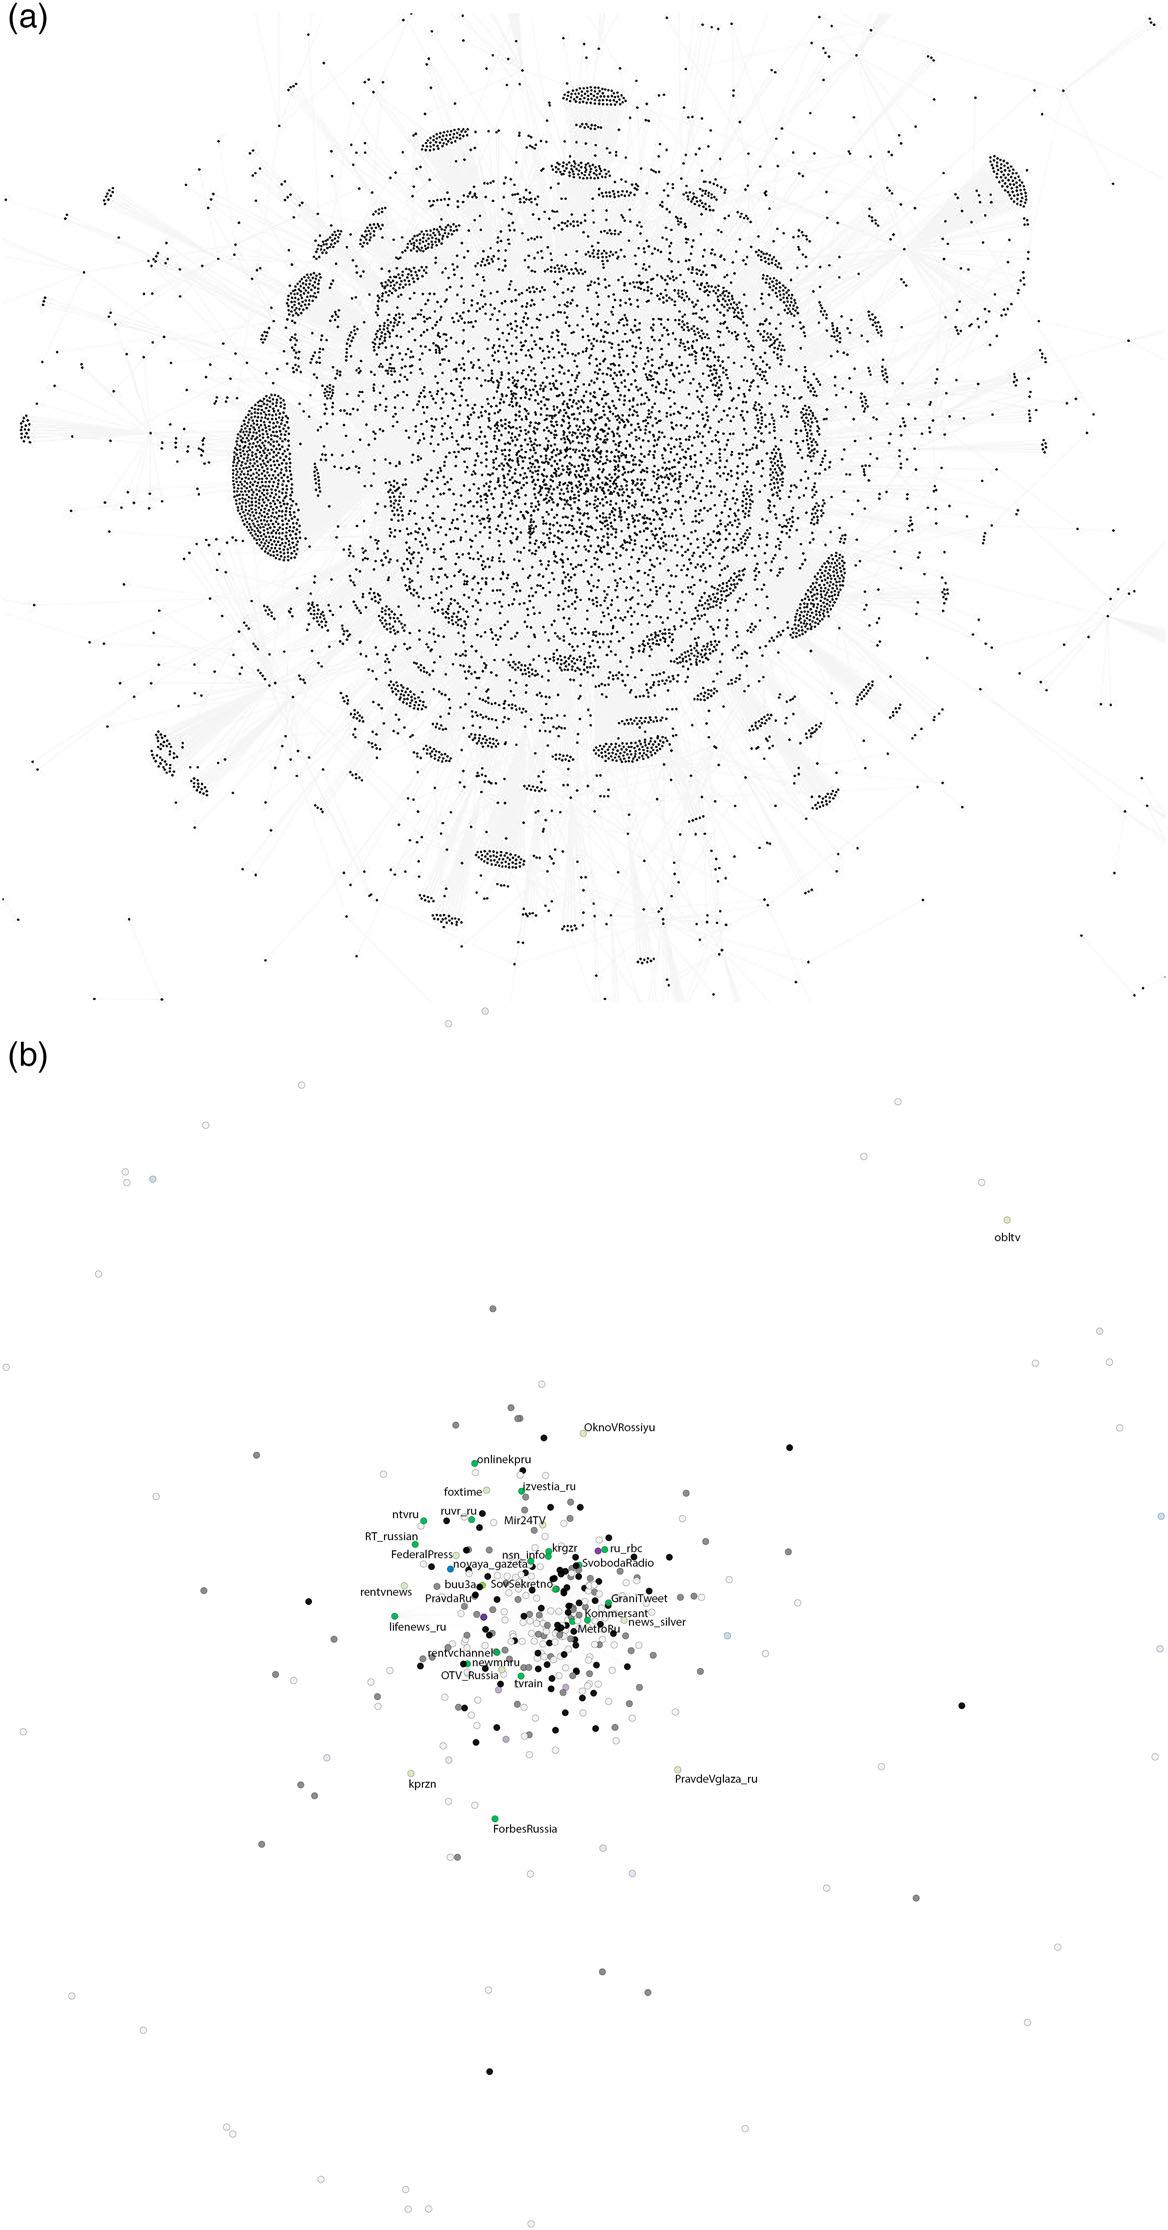
\includegraphics[scale=1.0]{webGraphsRussia}
	}
	\caption{Web graphs and influencers in the discussions on inter-ethnic conflicts in Russia: (a) the discussion graph; (b) the representation of top users by nine metrics.}\label{fig:webGraphsRussia}
\end{figure}

\clearpage

\begin{figure}[ht]
	\centerfloat{
		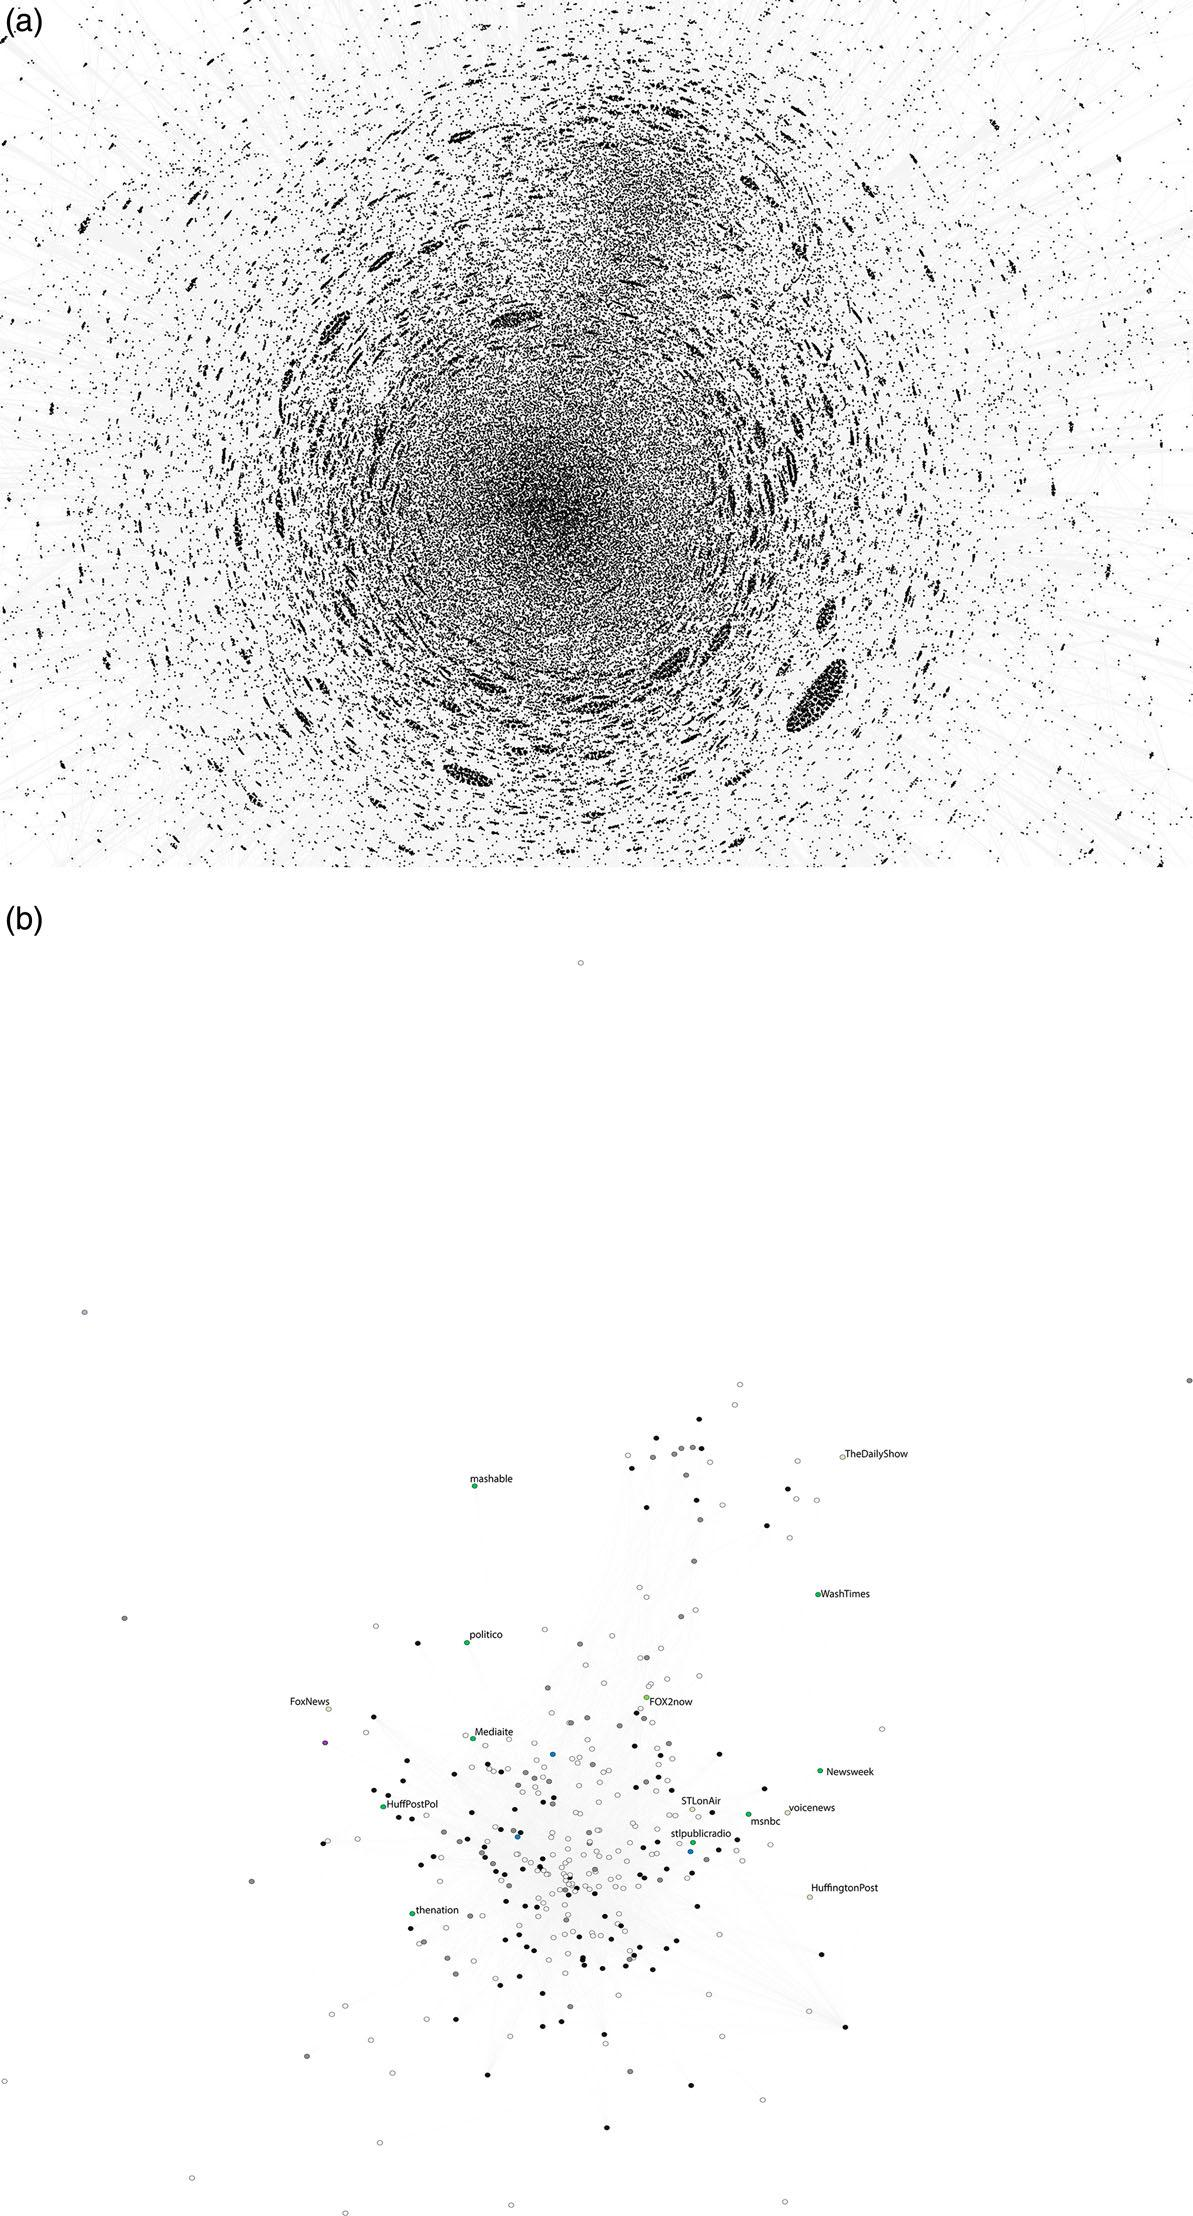
\includegraphics[scale=1.0]{webGraphsUS}
	}
	\caption{Web graphs and influencers in the discussions on inter-ethnic conflicts in the United States: (a) the discussion graph; (b) the representation of top users by nine metrics.}\label{fig:webGraphsUS}
\end{figure}

\clearpage

\begin{figure}[ht]
	\centerfloat{
		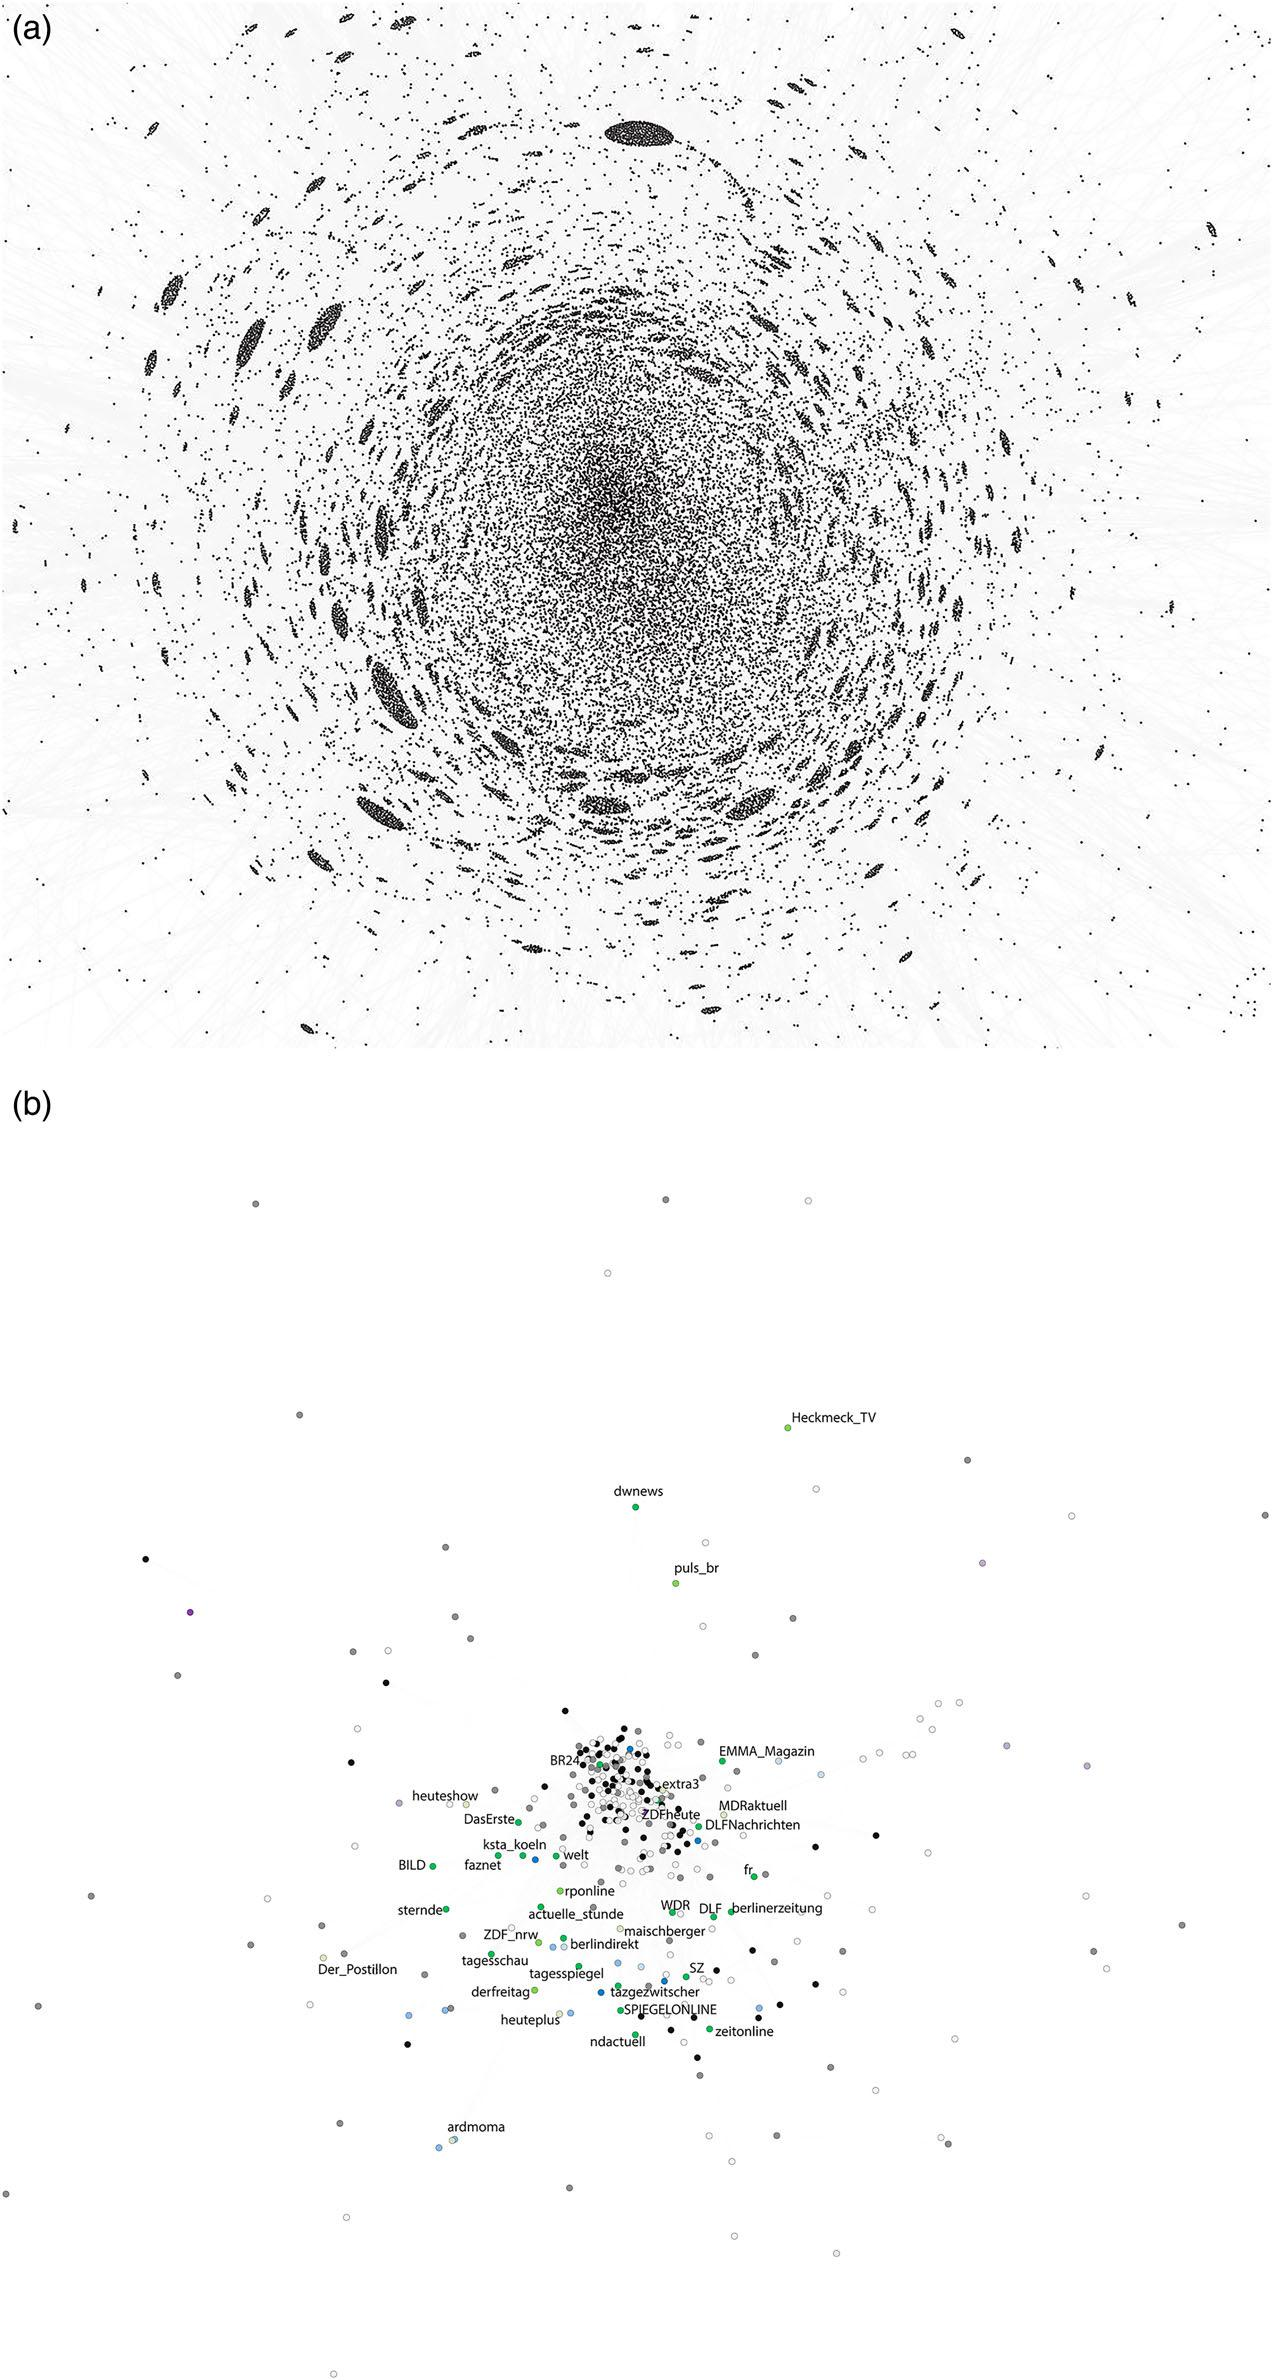
\includegraphics[scale=1.0]{webGraphsGermany}
	}
	\caption{Web graphs and influencers in the discussions on inter-ethnic conflicts in Germany: (a) the discussion graph; (b) the representation of top users by nine metrics.}\label{fig:webGraphsGermany}
\end{figure}

\clearpage

\begin{figure}[ht]
	\centerfloat{
		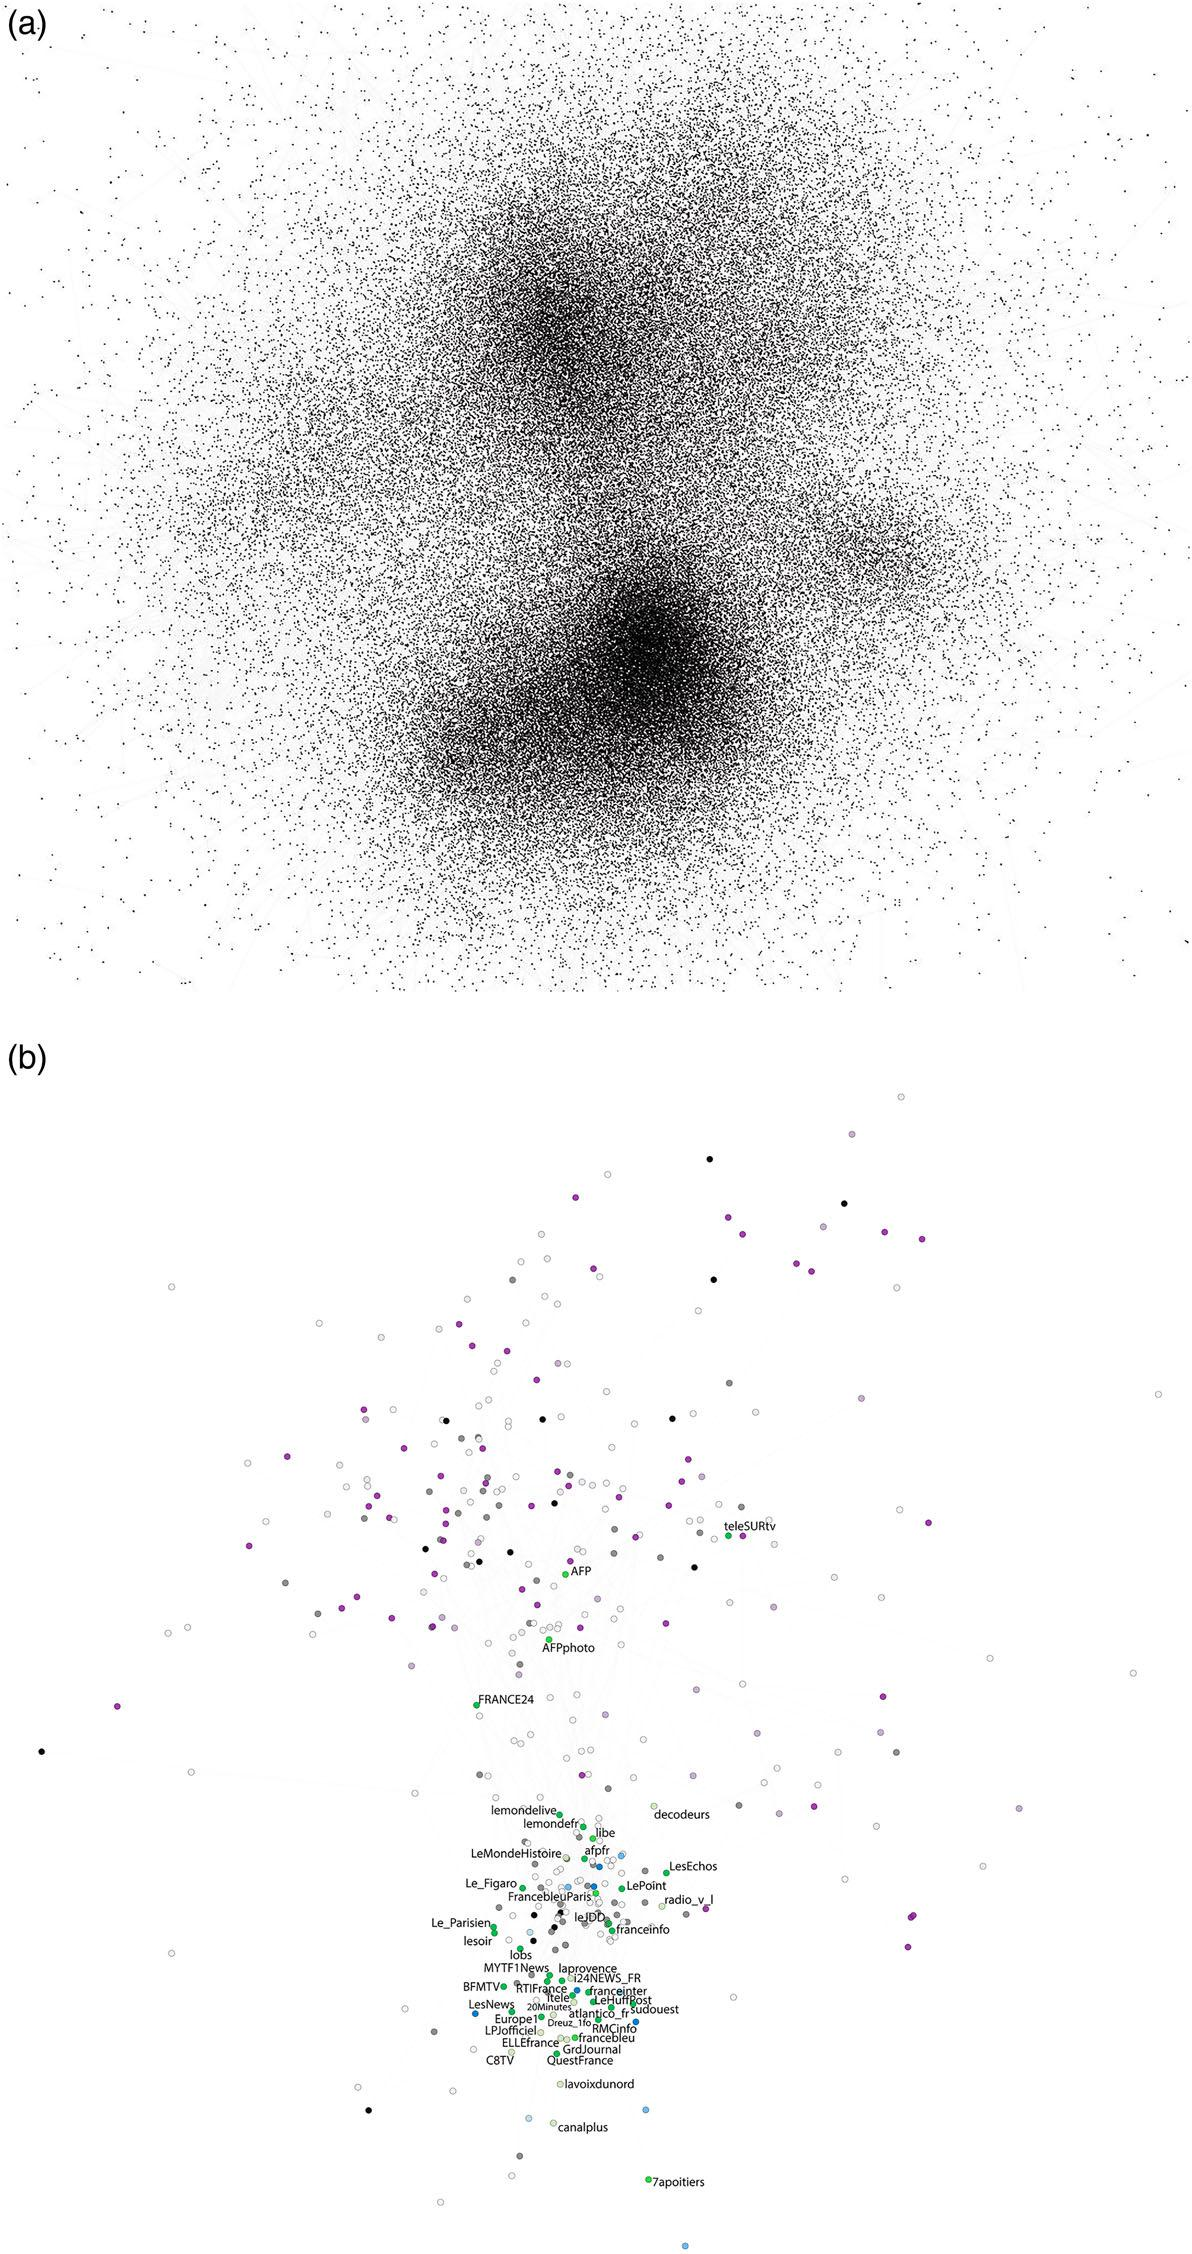
\includegraphics[scale=1.0]{webGraphsFrance}
	}
	\caption{Web graphs and influencers in the discussions on inter-ethnic conflicts in France: (a) the discussion graph; (b) the representation of top users by nine metrics.}\label{fig:webGraphsFrance}
\end{figure}

What we see in Figures~\cref{fig:webGraphsRussia,fig:webGraphsUS,fig:webGraphsGermany,fig:webGraphsFrance} adds to the pictures. As for Russia and the United States, we can see political polarization within the top-100 user graphs, especially in terms of the media. In Russia, there is a pro-state cluster (RT Russian, Voice of Russia, and two more outlets) and a liberal-oppositional cluster (including Radio Liberty in Russian and \textit{Novaya gazeta}). We also see that the pro-state \textit{Lifenews} news holding and the more liberal \textit{Forbes Russia} were important foci of discussion outside these clusters. In the case of Ferguson, polarization shows up in a different way, as the more left-leaning media, such as MSNBC, \textit{HuffPost Politics}, \textit{The Nation}, and \textit{Mediaite}, stand closer to the discussion center and are multi-role, while Fox News and its programs are more peripheral and single-role; the St. Louis media sit close to each other. In Russia, only a few media are positioned in the discussion center; in the United States and Germany, they sit around it, and, in the latter case, one may see a television news bulletin cluster, a neutral/left-leaning cluster (from \textit{Zeit} to \textit{Aktuelle Stunde}), a tabloid cluster (\textit{Bild} and \textit{Stern}), and a more conservative cluster (with \textit{Frankfurter Allgemeine Zeitung} and \textit{Die Welt}). The French case, in its turn, shows a huge presence of global media that form a sort of field quite separated from the French-speaking discussion core where some French media find their place, but most of them form a distinct cluster beside the main discussion nebula. Thus, we see that the capacity of normative role performance for media which are ranked high by centrality metrics may still be limited -- the media, indeed, are important nodes in the discussion, but they tend to result in grouping according to format and bias, which means they speak mostly to mini-audiences that prefer these biases and formats.

One more observation is worth noting. In the United States, Germany, and France, and, to a lesser extent, in Russia, the media sit either alone or in mini-clusters around the discussion core, forming a “second layer” around it. Thus, the assessment of graphs (a) and (b) suggests that we can talk about the roles of all media on the whole: all together, they link the discussion core to the periphery and provide the graph center with input for discussion. Moreover, most single-role media and those with low centrality rankings (even if high numbers of posts, likes, or shares) are situated farther from the discussion core than multi-role media. Thus, the relations between user centrality and role strategy on social networks deserve more investigation for both the media and journalists.

\subsubsection{Discussion}

The findings of the four case studies can obviously be generalized only to a certain extent. However, they show that combining network analysis and content analysis may help to better define today’s roles of the media and journalists online.

We have suggested defining media roles in online discussions by combining the percentage of opinionated content and the position of a given account by SNA metrics. The volume of opinionated content may be used as a hint for role performance -- information disseminators publish less than 30 percent of it, balanced interpreters up to 50 percent, and opinion propagators over 50 percent. We see this formal approach as suitable for assessing the strategies of individual media/journalist accounts, but it is also useful to look at the discussion graphs to see whether users gaining top ranking positions work as real opinion bridges or, vice versa, echo chamber centers.

We have seen that significant similarities exist in media strategies across Western and non-Western contexts, including Russia. Most legacy media tend to perform informing-oriented roles and are posting informational tweets. Often, the latter are announcements of news pieces designed for inviting Twitter users to follow them. However, more diverse strategies also exist, and European media tend to be similar in how they distribute between informing and opinion propagation.

At least two-thirds of the media in each country appear to reach the position of “authoritative informers” with multi-role performance. At the same time, in all the cases, there are media clusters divided due to format and bias, which is an obvious obstacle for performing the discursive roles efficiently. In all these respects, Russian media do not differ much from those of other countries.

We have also seen cross-cultural patterns of role performance based on format differences, but, unexpectedly, tabloid and regional media chose the same informing-oriented strategies as the quality media, while the entertainment media were more opinionated across the cases. Thus, the audience niche plays a less important role in defining media roles on Twitter than topicality and overall format (public affairs versus entertainment).

Journalists, unlike the media, have shown not only divergent but “polarized” strategies of role self-assignment, and this pattern is clearly present across countries and supports earlier findings by Lasorsa, Lewis, and Holton \cite{LasorsaLewisHolton} on the rise of journalists’ branding strategies.

Thus, our case studies have shown that Twitter has been “normalized” enough to show universal trends in media behavior within discussions on crises, but, in several aspects, national media markets and media traditions still prevail over the universality of Twitter. As we have found cross-national differences for ad hoc discussions, it may be important to apply the same research questions to “calm” periods in Twitter discussions.

Individual countries have also provided input for further research. Thus, the French case has demonstrated how the global media are entangled with the local media within a discussion; in Russia, the political alignment of the media influenced the role performance significantly; in the United States, the relative scarcity of media presence after just one week of the conflict was unexpected. These smaller findings may provide further grounds for comparative research, as well as research of the notion of the roles of the media community within online discussions.


\subsection{Multi-dimensional echo chambers: Language and sentiment structure of Twitter discussions on the Charlie Hebdo case}\label{subsec:ch5/sec1/sub3}

\subsubsection{1. Introduction}

Public discussions on social networks potentially have trans-border and multilingual nature. This comes true in heated conflictual discussions that reach global trending topics. Such discussions are expected to demonstrate ‘civilizational clashes’ \cite{AnKwakMejova}.

Being part of the global public sphere, since the 1990s, such discussions were expected by many observers to be more horizontal, all-involving, and democratically efficient \cite{Fuchs} than the traditional mass-mediated discussions \cite{McQuail}. But, with time, criticism towards the democratic quality of discussions in social media arose, with many works discovering the patterns of echo chambering and discourse polarization in social networks \cite{Sunstein2001,Sunstein2002,BarberaJostNagler,BastosMerceaBaronchelli,ColleoniRozzaArvidsson,ConoverRatkiewiczFrancisco}, which lowered the capacities of inter-group discussions and, thus, just formed an additional line of social segregation.

Object-oriented hashtagged discussions have been thoroughly studied in the 2010s, including those on political and social conflicts. But there is still scarce knowledge on whether affective hashtags \cite{Papacharissi} that convey emotions -- either of solidarity with or of anger towards a particular social group -- work in terms of user clusterization. Also, there is no clear understanding of comparative democratic quality of emotionally ‘positive’ and ‘negative’ hashtags in terms of echo chambering.

In this paper, we address these gaps by analyzing the Twitter discussion on the \textit{Charlie Hebdo} massacre of 2015. In the discussion upon the mass killings, the Twittershpere has created \#jesuischarlie and \#jenesuispascharlie -- two emotionally differing discussion clusters with, allegedly, opposite sentiments towards the journal’s ethics and freedom of speech; the hashtags soon became ‘role models’ for online solidarity towards the victims of terrorist attacks and anthropogenic disasters.

To analyze the echo chambering patterns in the two discussions, we have focused upon two levels of echo chambers. We were wondering whether echo chambers formed on the level of a hashtag (based on language use) and within a particular language (based on user sentiment of French-speaking users).
The remainder of the paper is organized as follows. Section 2 reviews the literature on echo chambering in social media. Section 3 presents our methodology and the conduct of the research. Section 4 presents our results and discusses them.

\subsubsection{2. User Groupings on Twitter and the Efficacy of Public Sphere}

\paragraph{2.1 Social Media and the Public Sphere: Echo Chambers vs. Opinion Crossroads}
Public sphere as a spatial metaphor for a complex of discussions and procedures with a public status and decision-making goals \cite{Kleinstuber} has been amplified by the appearance of social media in the 2000s. By 1990s, it had been established in the academic literature that mediatized public sphere with traditional media playing the role of information hubs was uneven and hardly efficient in terms of access to opinion expression, as whole social groups remained under-represented, and newsmakers privileged in comparison to \textit{vox populi}. With the appearance of social media, hopes arose that the new communicative milieus would foster horizontalization of communication and provide for democratization and higher political participation \cite{Fuchs}. Also, hopes for better understanding and resolution of non-political inter-group conflicts existed.

But with time, these hopes fainted, as offline disparities seemed to reproduce online, including political interests, race, gender, and other inequalities \cite{Daniels}; emotion and affect proved to rule the discourse \cite{Papacharissi}, with publics even in most democratically developed countries moving from diverse in opinion to dissonant and disconnected \cite{Pfetsch}. With the development of social network analysis (SNA) and its application to social media research, the question of the efficacy of the public discussions in social media \cite{BrunsHighfield} became linked to network and structural features of the discussions, such as the influencer status \cite{BodrunovaBlekanovMaksimov,BodrunovaLitvinenkoBlekanov2016} and clusterization of users also known as user polarization \cite{BarberaJostNagler,BastosMerceaBaronchelli} and echo chambering \cite{ColleoniRozzaArvidsson,ConoverRatkiewiczFrancisco}. Some evidence was also gathered on discussion sphericules forming on the global scale just as well as nationally \cite{CammaertsAudenhove}.

\paragraph{2.2 Why the Twitter Discussions Fragment: Linguistic Properties of Speech as Catalyzers of Echo Chambering}
In early studies of social networks and its users, authors interested in testing the ability of networks to pull together users from distant locations and weak ties linked geo- graphical distance with factors like residence of users and their language profile \cite{TakhteyevGruzdWellman}. This is why Twitter that enabled the (arguably) quickest possible information spread across locations and languages became a major attractor of scholarly attention \cite{LotanGraeffAnanny,HongConvertinoChi}. But despite the global reach of the platform, several studies have found that people were still connected locally on Twitter \cite{CammaertsAudenhove,YardiBoyd}.

Along with locality and residence, linguistic factors, arguably, play a major role in user grouping on the global scale. Thus, the language(s) used by the discussion participants is the first natural barrier that is expected to make users group together and communicate within their language-based echo chambers \cite{ChenTuZheng}, both on Twitter on the whole and within particular hashtags \cite{BastosPuschmannTravitzki}.

Other factors have also been discussed as the catalyzers of user grouping on Twitter. Among those, political attitudes lead the research agenda \cite{BarberaJostNagler,BastosMerceaBaronchelli}. Here, several ways to detect user clusterization exist. Of them, use of network or semantic proxies like friendship ties \cite{BarberaRivero}, patterns of following \cite{Rivero} and retweeting \cite{CalaisGuerraMeiraJrCardie}, content sharing \cite{ColleoniRozzaArvidsson,BakshyMessingAdamic} etc. is till today the most prominent; another is automated analysis of user sentiment, either in general or toward an issue/actor in question (object-oriented) \cite{ConoverGoncalvesRatkiewicz}.

But all these studies depict user groupings within a single dimension; our idea is to try and trace user groupings multi-dimensionally -- both on the level of a hashtag (based on language use) and within a language nebula (based on user sentiment).

\paragraph{2.3 The \textit{Charlie Hebdo} Case: Emotional Hashtags and User Groupings}
To search for multi-dimensional echo chambers, we have chosen the case of the \textit{Charlie Hebdo} massacre of 2015. Here, we could hypothesize that the existence of emotionally opposite hashtags (\#jesuischarlie and \#jenesuispascharlie) already creates enclaves within the general discussion on the case. Then, within the hashtags, several clusters based on language structure may exist. Then, on the third level, we will look whether within the language clusters sub-clusters of sentiment form. In general, our idea is to see how exactly the language clusters correspond to the sentiment clusters in each language and whether ‘positive’ users within one language are linked to such in another language, while ‘negative’ users also group across languages in a similar way. But here we present only preliminary results that check if the user clusters may at all be detected based on language and on sentiment within a language.

\paragraph{2.4 Research Hypotheses}

Thus, our hypotheses are the following:
\begin{itemize}
	\item H1a. Non-random user groups will be detected for both hashtags, as based on
	language use.
	\item H1b. \#jesuischarie will not differ from \#jenesuispascharlie in their language
	structure, as both hashtags have reached global trending topics and are expected to show ‘civilizational clashes’.
	\item H2a. Non-random user groups will be detected within one language (French), as based on positive and negative sentiment.
	\item H2b. \#jesuischarlie will differ from \#jenesuispascharlie in the grouping based on user sentiment, due to the emotional opposition of the hashtags themselves.
	\item H3. Multi-layer echo chambering may be detected in trans-border hashtagged discussions of global reach.
\end{itemize}

\subsubsection{3. Data Collection and Conduct of Research}

\paragraph{3.1 Data Collection and the Datasets}
Using a web crawler developed especially for the Twitter data collection, we gathered all the tweets published openly under the hashtags \#jesuischarlie and \#jenesuispascharlie (by separate crawls) within January 7 to 9, 2015, as these three days covered the active conflict (from the killings in the editorial office to the assailants’ death) when the users provided virtually millions of tweets for collection.

The collected datasets included: for \#jesuischarlie: 420,080 tweets; 266,904 tweeters; 719,503 users who interacted with the posted tweets (by likes, retweets, or comments); for \#jenesuispascharlie: 7,698 tweets; 5,466 tweeters; 17,872 users who posted and interacted with the posted tweets (by likes, retweets, or comments).

These full datasets were later used to reconstruct the overall web graphs for the two hashtags. But the datasets were very different in size, and be able to color them with language markers, we needed to sample the users for coding having in mind the volume difference of the datasets.

\paragraph{3.2 Language Analysis: Sampling, Coding, and Graph Reconstruction} 
To answer H1a and H1b, we have coded the users for their language use and then applied these data to the datasets for web graph reconstruction.

After eliminating bots and bot-like users (those who posted over 60\% of doubled tweets) as well as hashtag-only tweets, we have followed the strategy developed by the research group for previous Twitter studies \cite{Authors2016a,Authors2016b,Authors2018}, namely uniting random sampling with detection of influential users (influencers) for taking them into account. Then, we have coded all the influencers (disregarding the number of tweets they posted; for \#jesuiuscharlie, 402 users, for \#jenesuispascharlie, 85 users) and ‘ordinary users’ sampled in the feasible and comparable way. For \#jenesuispascharlie that was substantially smaller, all the users with 3 and more tweets were coded (339 users); for \#jesuischarlie, the ‘ordinary users’ with 5 tweets or more were taken into account (9,090 users), and of them, each second was coded (4500 users).

All the sampled underwent expert reading and were coded manually marking the number of tweets in language 1, language 2, and other languages; thus, users posting on one, two, and three or more languages were defined. The languages were identified for each user; in case of rare languages, Yandex language identifier was employed.

To reconstruct the graphs, we use Gephi API algorithms openly available online. Of the available algorithms, two were chosen: Hu \cite{Hu} and OpenOrd \cite{MartinBrownKlavans}; here, YifanHu-based graphs are presented, as the OpenOrd graphs require more space for presentation. We colored both the nodes (users) and the edges (connections between users). To prove that the visual nebulae are not artifacts of subjective viewership, we calculated the percentage of edges between and inside language groups, eliminating the ‘loops’ of self-commenting/liking by the users.

\paragraph{3.3 Sentiment Analysis: Sampling, Vocabulary Building, and Graph Reconstruction}After we have proved that the French-speaking users show non-random grouping in both cases (see below), we have taken them for sentiment analysis. The number of users for \#jesuischarlie included 1291 user; for \#jenesuispascharlie, 117 users.

Our strategy for French-language sentiment analysis was the following. We have united three sources in our vocabulary: the existing French dictionary with sentiment marking, machine translation from an additional Wordnet vocabulary, and the case-based vocabulary created from the collected tweets and manually marked for positive, negative, and neutral sentiment regardless of the case-specific meanings.

This vocabulary was applied to each tweet of the abovementioned French-speaking users; for each tweet, the sentiment was calculated. Then, the thresholds were defined: positive and negative were the users with positive(+neutral) and negative(+neutral) tweets, respectively; neutral were those with neutral tweets only; mixed were those with positive + negative(+neutral) tweets.

Then, we also checked the groupings with by calculating the percentage of edges both between and inside language groups, eliminating the ‘loops’ of self-commenting/liking by the users.

\subsubsection{4. Results and Discussion}

Our results are described below with regard to the hypotheses stated above.

\textit{H1a/H1b.} To assess the user groupings in both hashtagged discussions, we have reconstructed the web graphs for the coded users (see Fig.~\cref{fig:yifanHuGraphs-2} for \#jesuischarlie and Fig.~\cref{fig:yifanHuGraphs-2} for \#jenesuispascharlie, respectively). What we see on the graphs are three nebulae for~\cref{fig:yifanHuGraphs-1}: French, English, and other European, and two for~\cref{fig:yifanHuGraphs-2}: French and Engish. But the results of calculations of percentage of edges between and inside groups tell that the actual grouping is slightly different from what we see with unaided eyes. For \#jesuischarlie, the nebulae with density higher than the inter-group ones are French, English, and French/English (52.1\%, 16.7\%, and 16.9\%, respectively, against 6.17\% for inter-group edges) and not other European. For \#jenesuispascharlie, the graph is much denser (26\%), but still the same three clusters show up, with 26.2\%, 22.4\%, and 18.8\%, respectively; in both cases, other language clusters are virtually non-existent and do not mount to 3\%. As we stated in our earlier investigations \cite{Authors2018}, we have not seen a sign of ‘civilizational clashes’ in any of the hashtags.

\begin{figure}[ht]
	\centerfloat{
		\hfill
		\subcaptionbox[List-of-Figures entry]{\label{fig:yifanHuGraphs-1}}{%
			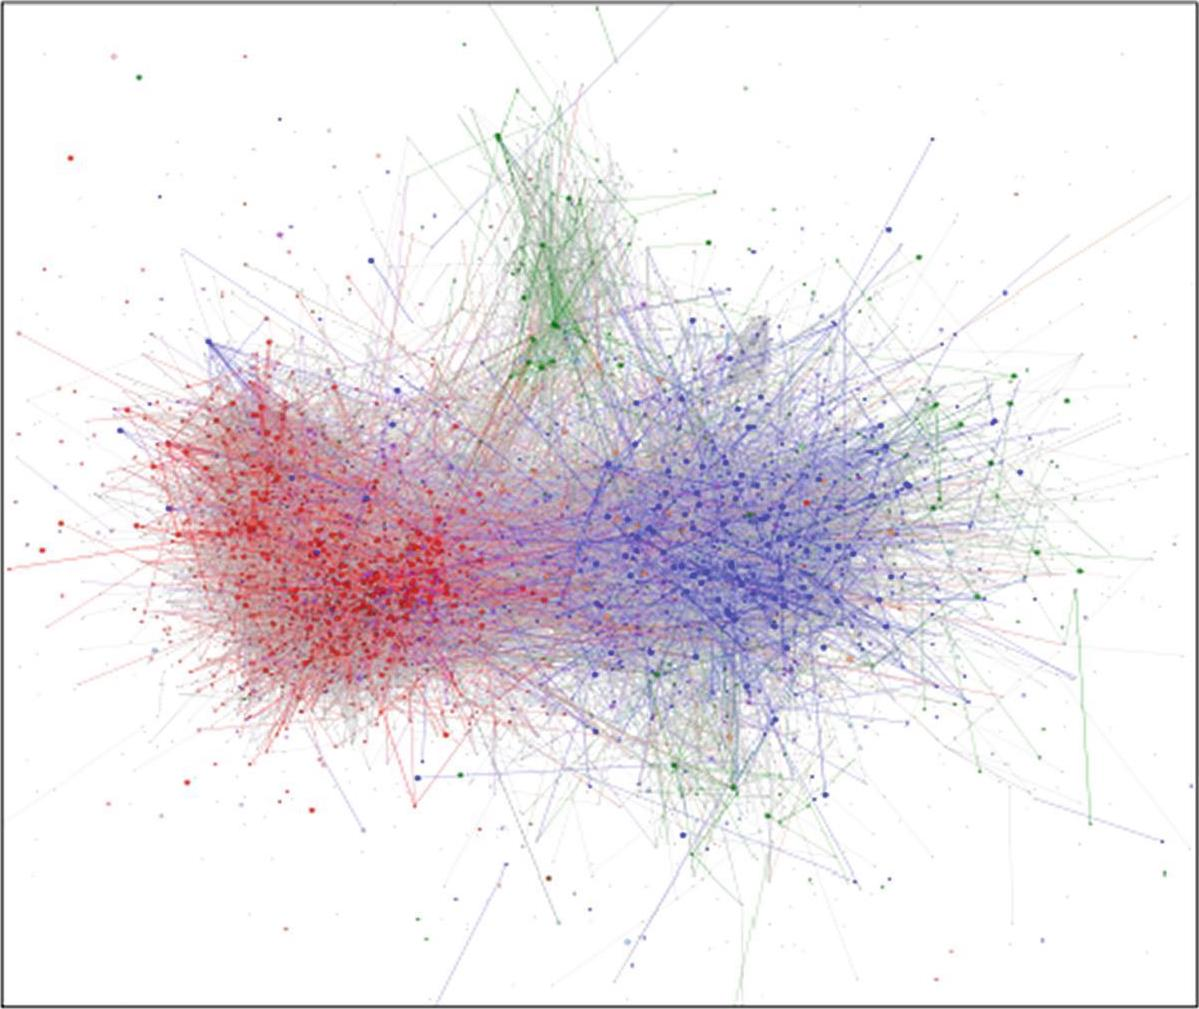
\includegraphics[width=0.419\linewidth]{yifanHuGraphs1}}
		\subcaptionbox{\label{fig:yifanHuGraphs-2}}{%
			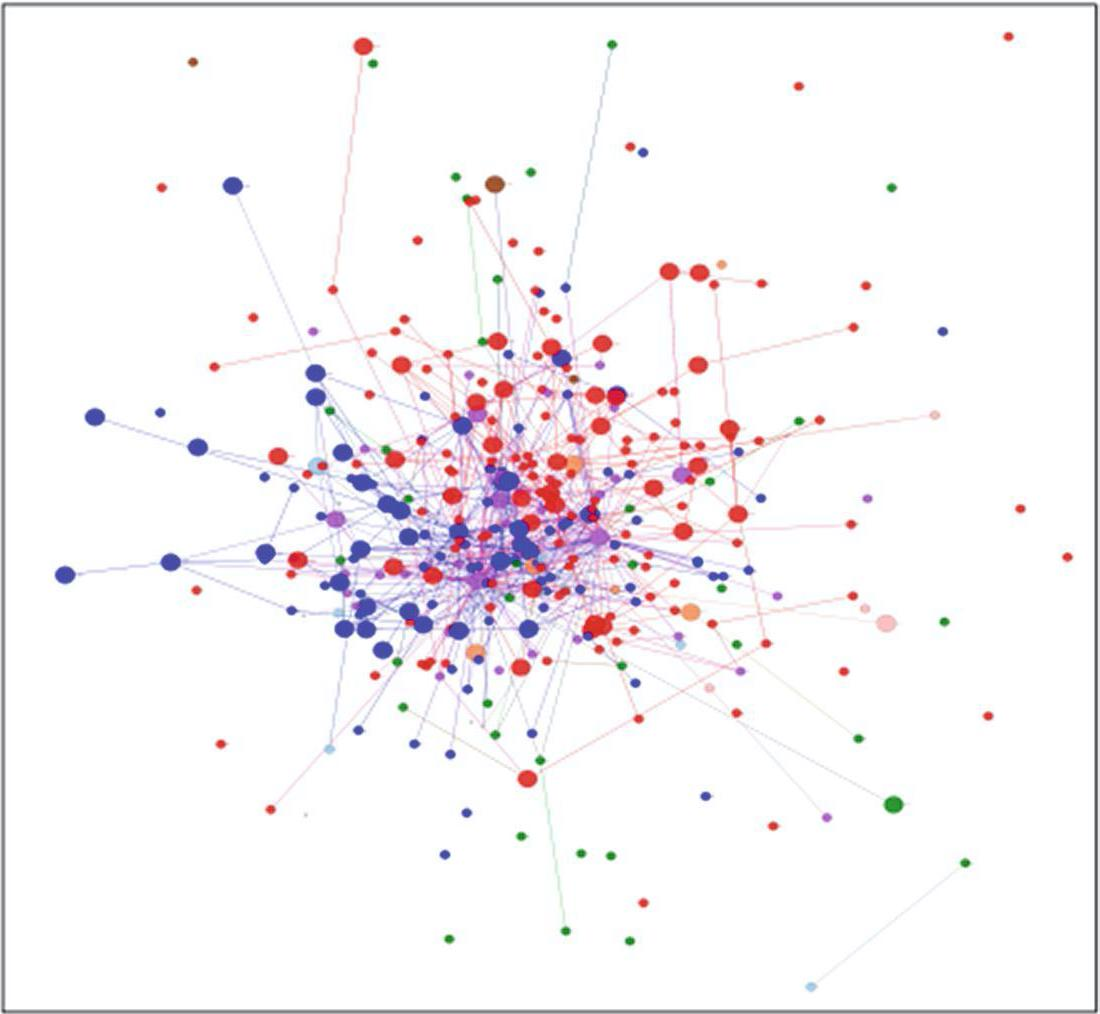
\includegraphics[width=0.382\linewidth]{yifanHuGraphs2}}
		\hfill
	}
	\caption{The YifanHu graphs (fragments) for language distribution in \cref{fig:yifanHuGraphs-1} \#jesuischarlie and \cref{fig:yifanHuGraphs-2} \#jenesuispascharlie. Red: French; blue: English; lilac: French/English; green: other European. (Color figure online)}\label{fig:yifanHuGraphs-12}
\end{figure}

Thus, H1a is proven; H1b is proven too but not due to ‘civilizational clashes’.

\textit{H2a/H2b.} To see the user grouping and sentiment cleavages within the French-speaking parts of the discussions, we have reconstructed the web graphs for them (see Fig.~\cref{fig:yifanHuGraphs-3} for \#jesuischarlie and Fig.~\cref{fig:yifanHuGraphs-4} for \#jenesuispascharlie, respectively).

\begin{figure}[ht]
	\centerfloat{
		\hfill
		\subcaptionbox[List-of-Figures entry]{\label{fig:yifanHuGraphs-3}}{%
			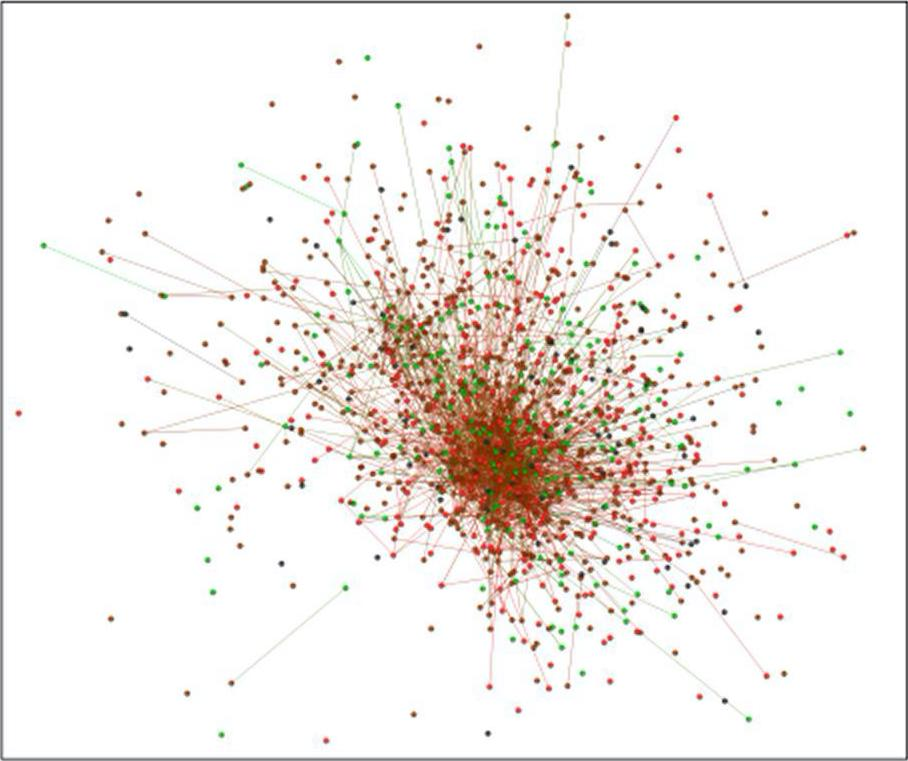
\includegraphics[width=0.419\linewidth]{yifanHuGraphs3}}
		\subcaptionbox{\label{fig:yifanHuGraphs-4}}{%
			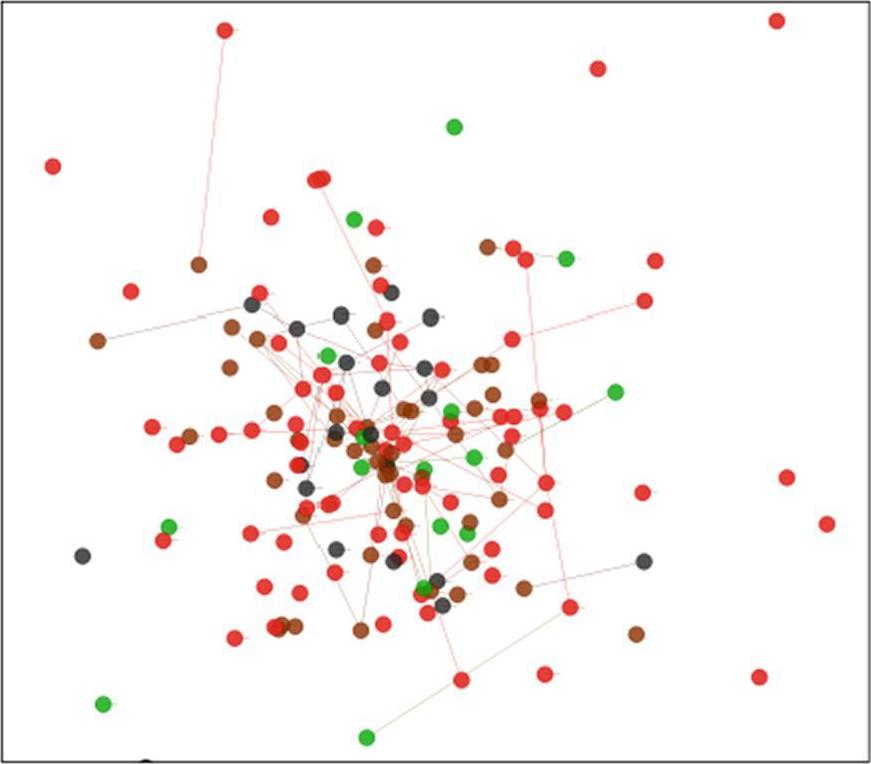
\includegraphics[width=0.4\linewidth]{yifanHuGraphs4}}
		\hfill
	}
	\caption{The YifanHu graphs (fragments) for language distribution in \cref{fig:yifanHuGraphs-3} \#jesuischarlie and \cref{fig:yifanHuGraphs-4} \#jenesuispascharlie. Red: French; blue: English; lilac: French/English; green: other European. (Color figure online)}\label{fig:yifanHuGraphs-34}
\end{figure}

Here, H2a should be rejected for \#jesuischarlie and partly supported for the second hashtag. Both in the graph and in the edge percentage calculations, it is only users with mixed sentiment who form a group (38.33\% against 56.05\% for the inter-group connections) in \#jesuischarlie. But for \#jenesuispascharlie, both mixed and negative user groups seem to have a potential for grouping (19.5\% and 15\% against 62.1\% for inter-group connections). Thus, H2b is supported: the cases do differ.

Even with the cases of such different sizes, H3 is supported: thanks to the negative nebula in \#jenesuispascharlie, we can state that echo chambers are able to form on at least two levels of the trans-border conflictual discussions of global (or, more precisely, macro-regional) reach. This adds to our understanding of the nature of public discussions in social media, even if lowers hopes for all-encompassing public spheres.

\subsection{Power laws in \textit{Ad Hoc} conflictual discussions on twitter. Digital Transformation and Global Society}\label{subsec:ch5/sec1/sub5}

\subsubsection{1. Introduction}

Public discussions online, and, of these, the ones on social networking sites, have become a growing area of scholarly attention, as they have been perceived as a manifestation of the public sphere, a crucial condition for efficient democratic deliberation \cite{Habermas}. Thus, understanding how networked discussions form and evolve is necessary for elaboration of proper criteria for their efficiency evaluation.

One of the issues recently raised by social science and communication scholars is that of comparability of the online discussions formed by the so-called issue publics \cite{Dahlgren}\cite[p.~422]{Habermas}. Such discussions form quickly (or even burst out) around events or burning issues. Due to their \textit{ad hoc} nature \cite{BrunsBurgess}, they may dissolve just as quickly, involve various actors, and are affective \cite{Papacharissi} and, thus, are shaped by emotions rather than by rational argumentation. The question remains whether we have grounds for comparing such discussions, as the differences in discussion substance may lead to critical differences in the discussion structure and connectivity, which would make, e.g., cross-cultural and cross-language comparisons of same-topic discussions impossible. Also, conclusions made for one discussion in terms of actor roles, dynamics, other constitutive parameters would not allow for predicting them for other discussions if the network structures are not assessed and recognized as similar.

This question has not yet been properly addressed in the social network analysis literature, as structural similarities of networked discussions, despite all the attention given to them, remain understudied in comparative perspective, especially in the view of the public sphere theory. The latter has elaborated its own vision of how to assess the efficacy of public discussions. Linking the two research areas for elaborating the SNA parameters for such assessment of the discussion networks would address one of the existing gaps in social network studies. For example, a number of more recent works have juxtaposed calculated and \textit{ad hoc} publics \cite{BrunsBurgess2015,LynnRosatiNair} in search of networking patterns of both types of discussions, but these studies were single-case, and we still lack the knowledge whether structural patterns vary across cases, cultures, and types of vocabularies used for data collection.

Another input for social network analysis from the public sphere theory would be addressing the difference between users who are key for the discussion outburst and random discussion participants. Traditional view would imply various manifestations of power distance between the two user groups, and one needs to know whether online discussions show stable patterns of differences between key and random users.

We address these research gaps by collecting data and analyzing web graph structures for five discussion outbursts about inter-ethnic (inter-national and inter-race) conflicts in the USA, Germany, France, and Russia of the 2010 s, reviewing altogether six discussion cases, as we split one into neutral and affective parts. We collect data from Twitter based on single hashtags and keyword conglomerates and show that there are repeatable structural patterns of the discussions across these cases.

The remainder of the paper is organized as follows. Section 2 discusses today’s literature on various aspects of discussion structure for comparative tasks. In Sect. 3, we describe the cases and formulate the hypotheses for their comparison. Section 4 shows and discusses the discovered results. In conclusion, we discuss applicability of our findings for further studies of online conflictual discussions.

\subsubsection{2. Comparing Discussion Structure on Social Networks: A Literature Review}

Ad hoc \textit{discussions: a plea for grounds for comparison}. Public discussions on social networking sites have drawn scholarly attention to their various aspects, including the connection between the deliberative power of ‘ordinary citizens’ and the platform and network features that might either empower or disempower user groups in their opinion expression, shape the discussion outcomes, and impact the respective decision-making, as well as inspire political mobilization via the ‘logic of connective action’ \cite{BennettSegerberg}. Thus, the discussions in online networks have been thoroughly studied in their substantial aspects. But one of the key issues in this research area is the principal possibility of comparisons between discussions on similar topics happening in various parts of the world and in varying times.

So far, comparative studies of cross-country social network discussions have been rare \cite{BodrunovaLitvinenkoBlekanov2017}; one of the reasons for that is the scholarly argument of low (or, rather, unknown) comparability of the discussions that are formed by the issue publics. This type of the discussion raises, arguably, the biggest amount of doubt ‘whether Habermas is on Twitter’ \cite{BrunsHighfeld2016}, as, from case to case, current research demonstrates varying results on echo chamber formation \cite{BastosMerceaBaronchelli,ColleoniRozzaArvidsson,Sunstein2001,YardiBoyd}, cross-group discussion potential \cite{Barbera,BarberaJostNagler}, and the roles of influencers detected by various means \cite{BastosRaimundoTravitzki,BodrunovaLitvinenkoBlekanov2017,DuboisGaffney}.

The reason for low comparability, as scholars argue, lies in the very nature of the discussions, as they are all \textit{ad hoc} -- that is, case-specific and random in formation. Such discussions have the outburst nature, may have varying patterns of dissolution, involve case-specific actors, and based on affect \cite{Papacharissi} -- that is, are shaped by emotions rather than by rational argumentation, which may add to the non-comparability of the discussions. Thus, the major research question is -- are \textit{ad hoc} discussions comparable in topical and sociological terms also comparable in the discussion structures? Or, in other words, are there structural features characteristic of such discussions, that would, ideally, distinguish them from other discussion types on social networks and on the Web on the whole? And what could be the markers for such \textit{ad hoc} discussion outbursts?

Today, in Twitter studies, there is scarce but growing evidence that \textit{ad hoc} discussions differ in their nature from other discussion types. Thus, several papers underline the differences between calculated and \textit{ad hoc} publics \cite{BrunsBurgess2015,LynnRosatiNair}, but no network parameters were used to prove the differences between these discussion types. Also, these studies were based on single cases, and we still lack the knowledge whether structural patterns for \textit{ad hoc} discussions vary or repeat across cases, cultures, and types of vocabularies used for data collection. This creates a focus for our enquiry.

\paragraph{Degree centralities as a proxy for discussion comparability and a potential discussion quality metric.} Degree centralities (in-degree, out-degree, and degree accumulating both of these) have been long ago recognized as the key structural metrics of user relations and random graph assessment \cite{AlbertBarabasi,BoccalettiLatoraMoreno,MisloveMarconGummadi}; degree distributions are recognized as a key variable describing users’ interest toward each other \cite{EdigerJiangRiedy}. At the same time, from the normative viewpoint relevant in social sciences, degree centralities are an important metric of user in-network influence \cite{BodrunovaLitvinenkoBlekanov2016}, as well as the metric important in deliberative terms: the more users are reached by the same user (or reach a given user, which is the same for non-directed graphs but not for directed graphs), the more probable is the chance for cross-opinion discussion. More importantly, it can also characterize general user involvement into the discussion in comparison with other discussions; in terms of user involvement, degree centralities are, arguably, the most telling. A range of more topic-specific research papers have also argued that degree-based metrics are useful for network-based studies of social conflict and dangerous networks. Of those, one work \cite{KarthinkaGeethaBose} has shown the importance of relational measures (as the authors noted, ‘who is related to whom’) in detecting the key attackers in the terrorist network.

There are, of course, several criticisms about degree distributions, as they gener- alize the network structure without taking into account the role of influencers (for the reviews on detecting and comparing influencer structures, see \cite{BodrunovaBlekanovMaksimov,BodrunovaLitvinenkoBlekanov2017,BodrunovaLitvinenkoBlekanov2016}), or ‘hub users’. Their roles, in various works, are assessed in different, if not directly opposite, ways. Thus, one stream of works insists on their disproportionately big role in information distribution (see \cite{BastosRaimundoTravitzki,DuboisGaffney}, and many others), while another line shows that such hubs may be inefficient due to their overload and incapability of transmitting information due to that \cite{HarriganAchananuparpLim}. But our goal is to test whether the discussions on the whole may be distinguished from Twitter on the whole.

As major research works in the area note \cite{BarabasiAlbert,BroderKumarMaghoul,HubermanAdamic}, due to preferential connectivity in real-world networks, a certain power law (just as its absence) in degree distribution may become the characteristic that describes specific network structures. Thus, networks expressing power-law-like degree distributions are known as scale-free \cite{AlbertBarabasi,EdigerJiangRiedy}, and ‘scale-free tweet mention graphs would imply that a few Twitter users and ‘mentioners’ are responsible for a disproportionately high fraction of a community’s discourse’ \cite[p.~587]{EdigerJiangRiedy}. Thus, degree distribution may serve as a proxy for, e.g., core vs. periphery assessment in terms of aggregate influencer power: it can tell whether the network is dominated by a small number of users \cite{YeWu}. Thus, for Twitter, it would allow for: (1) differentiating one network type from another; (2) proving that the discussions are similar in their core vs. periphery relations, which suits our research goals. Moreover, our previous studies \cite{BlekanovSergeevMaksimov2017} have shown that power law exponents, indeed, vary for different types of web structures; e.g. for university websites, the average exponent is 1.8 instead of the expected 2.1.

Early works on World Wide Web topology mentioned above, as well as other research papers (see, e.g., \cite{FaloustosFaloustosFaloustos}), all stated that power law distributions are characteristic for the Web on the whole. But another, later line of research papers has argued that the Web, by just evolving in time, has blurred the initial power-law-like degree distribution \cite{ChenChangGovindan,MeuselVignaLehmberg}. Smaller-scale research, though, tells that degree distributions are still valid for smaller real-world samples.

Today, more and more criticism is raised about the explanatory potential and the very existence of scale-free networks -- that is, of the power law in degree distributions -- in large human-based datasets \cite{BroidoClauset}. We, thus, want to test whether the certain power laws show up in ad hoc discussions, as distinguished from Twitter on the whole, cultivated long-term discussions, and random talk.

\paragraph{Power laws on Twitter: lack of comparative studies on the nature of the discussions.} So far, degree distributions have been studied for either the whole Twittersphere or its geographical segments; and, in these studies, the evidence on whether all the discussions on Twitter manifest power-law degree distributions is mixed.

Thus, cumulative degree distributions \cite{Newman} for Twitter on the whole studied a decade ago \cite{JavaSongFinin} showed that the slopes cin and cout [were] both approximately \(-2.4\). The authors have interpreted these figures as similar to those for the Web of those times (\(-2.1\) for in-degree, cf. \cite{DonatoLauraLeonardi}) and blogosphere (\(-2,38\), as based on Blogpulse conference dataset of 2003). With the latter claim, one could agree, but with the former one we would not, as our research shows that differences of 0.3 in exponent values may be characteristic of graph origin and/or discussion type \cite{BlekanovSergeevMaksimov2017}. Another study \cite{WengLimJiang} based on the data dated mostly from April 2008 to April 2009 and featuring the most followed Twitter users from Singapore has also demonstrated power-law-like degree distributions of the user networks. A Twitter-large study \cite{WelchSchonfeldHe} has shown a very different exponent value of \(-1.6\). But authors \cite{KwakLeePark} have crawled the whole Twittersphere and have not discovered any power law in link distribution on the global level, as other authors underline \cite{HansenArvidssonNielsen}.

Several studies have focused on country-based segments of Twitter. Thus, one study \cite{MyersSharmaGupta} has dealt with the Twitter follow graphs. The researchers have shown that in-degree and degree on Twitter are best fit by power law, while out-degree is best fit by log-normal distribution. Besides analyzing the entire Twitter, it also did country- based segment studies for Brazil, Japan, and the United States; very little variance was found between the countries in terms of in-degree, out-degree, and degree distribution \cite[p.~494]{MyersSharmaGupta}. Another study has dealt with the follow graphs of 10 country-bound Twitter segments around the world \cite{PobleteGarciaMendoza}. It has also demonstrated power-law in-degree and out-degree distributions, with power law coefficient ranging 5.91 to 9.51 and 8.12 to 13.62, respectively. But one also needs to note that user influencer status is linked much more to the number and activity levels of active followers (who retweet and/or mention a given user) than to the number of followers \cite{ChaHaddadiBenevenuto}; thus, one needs to look at the actual discussion graphs rather than at the graphs of following (much less linked to the real-world issue-based discussions) to more precisely determine the influential users, as well as to define the discussion type.

Even a fewer number of works have examined the degree distributions in hash- tagged discussions. We can name one work \cite{ZhouBandariKong} on Iranian elections; the discussion there also showed power law distributions, with in-degree being \(-2.85\) and out-degree being \(-2.42\), while the retweet-based network had in-degree of \(-1.94\). Another group of authors \cite{ConoverRatkiewiczFrancisco} have also observed that retweet- and mention-based networks virtually did not differ in their scale-free topology.

From the review above, one can conclude that scholarly evidence for power laws in degree distributions is greater than that of the opposite. But, despite their potential, degree distributions have not been tested for \textit{ad hoc} discussion outbursts in comparative perspective.

Our idea is to look how degree distributions work if we step-by-step eliminate the users with low degree index, starting from isolate users \((D = 0\)), and look at the cumulative degree distributions for each case.

\subsubsection{3. The Research Methodology}

\paragraph{The research questions.} Most of the available research proves that power laws are characteristic for Twitter ‘calm’ discussions, be it the whole Twitter or its parts, either hashtag-based or limited by region. But the exponent values of degree distribution vary highly, not allowing for any particular expectation. Thus, we ask: Will degree distribution of all the \textit{ad hoc} discussion be fit by a power law? Will the exponent values be similar, thus indicating that the discussions are similar? Will the exponent values differ from \(\lvert2.1\rvert\)? Will the exponent values be similar enough across world regions, hashtag- only / keyword conglomerates, and neutral / affective hashtags?

The research hypotheses that emerge of these research questions look as follows:

\begin{itemize}
	\item H1. All the discussions under scrutiny will be characterized by power law in degree distribution.
	
	\item H2. All the discussions will diverge from the \(\lvert2.1\rvert\) exponent value to the same direction and on comparable percentage. This includes hashtag vs. keyword conglomerates (H3).
	
	\item H4. Neutral and affective (expressing emotions of either sympathy and compassion or negation and hatred) hashtags will be comparable in their power law exponents.
\end{itemize}

\paragraph{The cases under scrutiny and their substantial comparability.} The cases of our attention all have the same set of features that is to ensure that the cases are comparable in sociological terms. Thus, all the cases have a violent trigger (a killing or rape/harassment) of inter-ethnic nature; the discussions are outburst -- that is, the number of users involved has one sharp peak and then slows down gradually; media report the communities to split into the minority, pro-minority majority, and anti-minority majority groups; there is peaceful protest or mass commemoration of the victims in the aftermath of the conflict; there is direct involvement of authorities of several levels into conflict resolution; and all the conflicts provoke a discussion on Twitter that gets to national (sometimes also to global) Twitter trending topics.

We are looking at the following cases (in chronological order):
\begin{itemize}
	\item A killing of a Russian Muscovite by an Uzbek immigrant and the subsequent anti- immigrant clashes in the Moscow district of Biryuliovo, Russia (2013);
	\item A killing of an African American teenager by a white police officer and the sub- sequent city riots in Ferguson, the USA (2014);
	\item The attack to the editorial office of Charlie Hebdo and the subsequent peaceful demonstrations in Paris, France (2015);
	\item The mass harassment of German females by male re-settlers from Middle East and North Africa in the New Year Eve in Cologne, Germany (2015--2016), and the subsequent protest meetings by PEGIDA and the ‘Alternative for Germany’ party;
	\item A bus attack at one of the Christmas markets in Berlin (2016).
\end{itemize}

In each case, the discussion data were collected and the respective web graph reconstructed; in the case of \textit{Charlie Hebdo}, two graphs (one for a neutral hashtag and one for a compassion hashtag) were reconstructed.

\paragraph{Data collection.} To collect the discussion bulk, we have created a specialized web crawler with adjustable modules \cite{BlekanovSergeevMartynenko}. It was done especially to overcome the well-known Twitter API limitations, like the ones on the number of requests to server and on the number of tweets available for download. It also bypasses the popularity algorithm and allows for human-like backfolding.

For bigger-scale discussions (Ferguson and Charlie Hebdo), one hashtag per graph was used. For smaller-scale discussions, snowballing reading of 1.000+ random tweets containing the primary hashtag/keyword was performed, thus bringing on keyword collections.

\begin{table} [htbp]%
	\centering
	\caption{The datasets collected.}%
	\label{tab:collectedDatasets}% label всегда желательно идти после caption
	\renewcommand{\arraystretch}{1.5}%% Увеличение расстояния между рядами, для улучшения восприятия.
	\begin{SingleSpace}
		\begin{tabulary}{\textwidth}{@{}>{\zz}L >{\zz}C >{\zz}C@{}} %Вертикальные полосы не используются принципиально, как и лишние горизонтальные (допускается по ГОСТ 2.105 пункт 4.4.5) % @{} позволяет прижиматься к краям
			\toprule     %%% верхняя линейка
			The case & The number of nodes & The number of edges \\
			\midrule %%% тонкий разделитель. Отделяет названия столбцов. Обязателен по ГОСТ 2.105 пункт 4.4.5
			Biryuliovo, 2013 & 11429 & 20106 \\
			Ferguson, 2014 & 169677 & 334050 \\
			\textit{Charlie Hebdo}, 2015 (neutral) & 952615 & 1782863 \\
			\textit{Charlie Hebdo}, 2015 (affective) & 719503 & 981131 \\
			Cologne, 2015--2016 & 40117 & 98508 \\
			Berlin, 2016 & 194937 & 298562 \\
			\bottomrule %%% нижняя линейка
		\end{tabulary}%
	\end{SingleSpace}
\end{table}

The initial datasets collected are represented in Table~\cref{tab:collectedDatasets}. Altogether, tweets by over 2 mln users were included into the research. Edges between the users were formed if any type of substantial interaction emerged between them (we counted retweets, mentions, and comments as such).

\paragraph{Web graph reconstruction and analytics.} We have reconstructed the graphs for each case. The graphs were non-directed, as we were interested in the aforementioned deliberative aspects of the discussions. We have used the OpenOrd algorithm for the graph reconstruction. This methods is based on calculating the maximum distance (in \%) between the two nodes and on a particular number of iterations (in all our cases, the algorithm converged the proposed 800 iterations to 750). This algorithm was chosen, as it brings to the discussion core (that is, to the center of the graph) the influential users defined by a wide set of variables, including absolute-figure ones (the number of tweets, likes, retweets, mentions, and comments) and centrality metrics (including degree, betweenness, parerank, and eigenvector centralities).

Then, the degree distribution exponents were calculated for each case, using eleven steps of isolate user elimination (for users with \(D = 0\) to 10 in the initial graph).

The results and answers to our hypotheses are presented below.

\subsubsection{4. The Research Methodology}

As stated above, we have calculated degree distribution exponents for each case. In order to clearly highlight the differences with the expected exponent value of \(\lvert2.1\rvert\) based on previous Web studies, we have also calculated the exponents for the eliminated users. The exponent values for both active users and eliminated users, as well as their absolute deviations from \(\lvert2.1\rvert\), are presented in Table 2. The degree distribution graphs are presented in Figs.~\cref{fig:biryuliovoDegreeDistribution},~\cref{fig:fergusonDegreeDistribution},~\cref{fig:charlieNDegreeDistribution},~\cref{fig:charlieADegreeDistribution},~\cref{fig:cologneDegreeDistribution} and~\cref{fig:berlinDegreeDistribution} for the respective cases, as ordered in Table~\cref{tab:caseExponentValues}.

\begin{table} [htbp]%
	\centering
	\caption{Exponent values for the cases and their divergence from the expects exponent value.}%
	\label{tab:caseExponentValues}% label всегда желательно идти после caption
	\renewcommand{\arraystretch}{1.5}%% Увеличение расстояния между рядами, для улучшения восприятия.
	\begin{SingleSpace}
		\begin{tabulary}{\textwidth}{@{}>{\zz}L >{\zz}C >{\zz}C >{\zz}C >{\zz}C@{}} %Вертикальные полосы не используются принципиально, как и лишние горизонтальные (допускается по ГОСТ 2.105 пункт 4.4.5) % @{} позволяет прижиматься к краям
			\toprule     %%% верхняя линейка
			The case & Exponent value, active users &  Absolute deviation, active users & Exponent value, eliminated users & Absolute deviation, eliminated users \\
			\midrule %%% тонкий разделитель. Отделяет названия столбцов. Обязателен по ГОСТ 2.105 пункт 4.4.5
			Biryuliovo, 2013 &  \(\lvert1.56\rvert \) & 0.54 & \(\lvert2.04\rvert\) & 0.06 \\
			Ferguson, 2014 & \(\lvert1.39\rvert\) & 0.71 & \(\lvert2.16\rvert\) &\( -0.06\)      \\
			\textit{Charlie Hebdo}, 2015 (neutral) & \(\lvert 1.59 \rvert\) & 0.51 & \(\lvert2.01\rvert\) & 0.09 \\
			\textit{Charlie Hebdo}, 2015 (affective) & \(\lvert1.80\rvert\) & 0.3 & \(\lvert2.45\rvert\) & \(-0.35\) \\
			Cologne, 2015--2016 & \(\lvert1.28\rvert\) & 0.82 & \(\lvert1.91\rvert\) & 0.19 \\
			Berlin, 2016 & \(\lvert1.63\rvert\) & 0.47 & \(\lvert2.34\rvert\) &  \(-0.24\) \\
			\bottomrule %%% нижняя линейка
		\end{tabulary}%
	\end{SingleSpace}
\end{table}

\begin{figure}[ht]
	\centerfloat{
		\hfill
		\subcaptionbox[List-of-Figures entry]{\label{fig:biryuliovoDegreeDistribution-1}}{%
			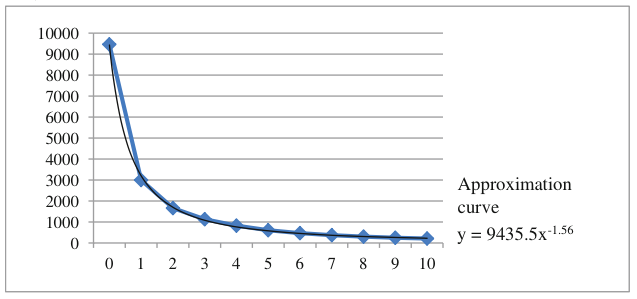
\includegraphics[width=0.5\linewidth]{biryuliovoDegreeDistribution1}}
		\subcaptionbox{\label{fig:biryuliovoDegreeDistribution-2}}{%
			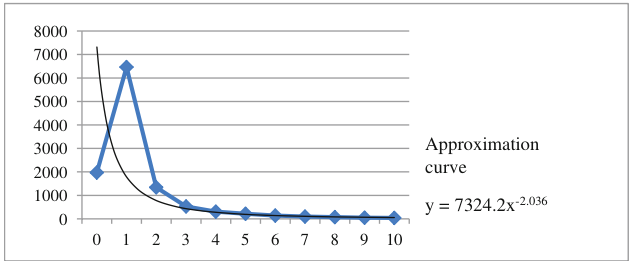
\includegraphics[width=0.56\linewidth]{biryuliovoDegreeDistribution2}}
		\hfill
	}
	\caption{Degree distributions for the Biryuliovo case: (а) active users; (б) eliminated users. \textit{Source:} authors.}\label{fig:biryuliovoDegreeDistribution}
\end{figure}

\begin{figure}[ht]
	\centerfloat{
		\hfill
		\subcaptionbox[List-of-Figures entry]{\label{fig:fergusonDegreeDistribution-1}}{%
			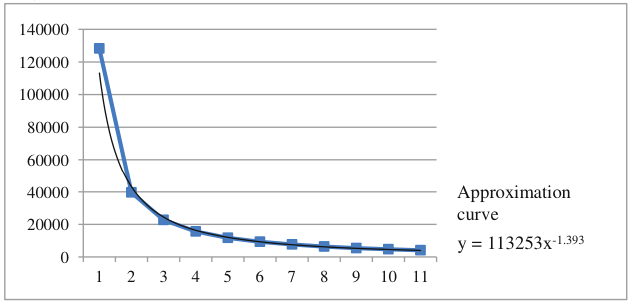
\includegraphics[width=0.509\linewidth]{fergusonDegreeDistribution1}}
		\subcaptionbox{\label{fig:fergusonDegreeDistribution-2}}{%
			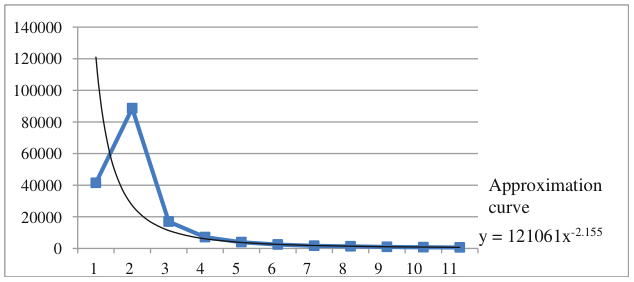
\includegraphics[width=0.55\linewidth]{fergusonDegreeDistribution2}}
		\hfill
	}
	\caption{Degree distributions for the Ferguson case: (а) active users; (б) eliminated users. \textit{Source:} authors.}\label{fig:fergusonDegreeDistribution}
\end{figure}

\begin{figure}[ht]
	\centerfloat{
		\hfill
		\subcaptionbox[List-of-Figures entry]{\label{fig:charlieNDegreeDistribution-1}}{%
			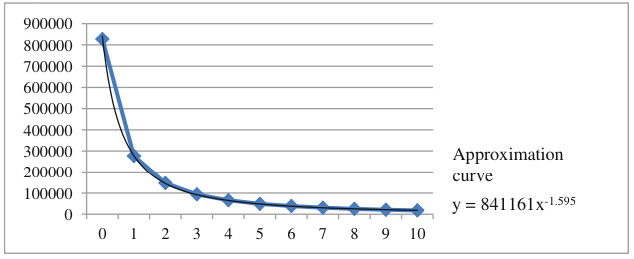
\includegraphics[width=0.56\linewidth]{charlieNDegreeDistribution1}}
		\subcaptionbox{\label{fig:charlieNDegreeDistribution-2}}{%
			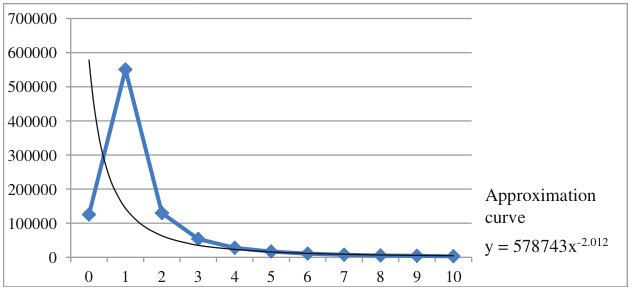
\includegraphics[width=0.5\linewidth]{charlieNDegreeDistribution2}}
		\hfill
	}
	\caption{Degree distributions for the \textit{Charlie Hebdo} neutral case: (а) active users; (б) eliminated users. \textit{Source:} authors.}\label{fig:charlieNDegreeDistribution}
\end{figure}

\begin{figure}[ht]
	\centerfloat{
		\hfill
		\subcaptionbox[List-of-Figures entry]{\label{fig:charlieADegreeDistribution-1}}{%
			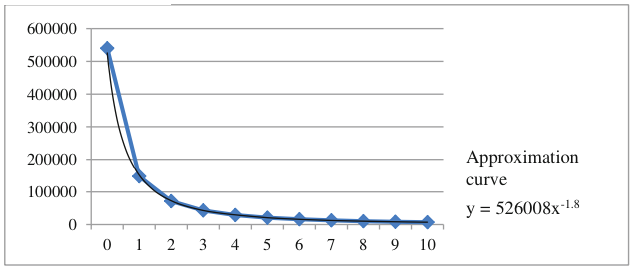
\includegraphics[width=0.5\linewidth]{charlieADegreeDistribution1}}
		\subcaptionbox{\label{fig:charlieADegreeDistribution-2}}{%
			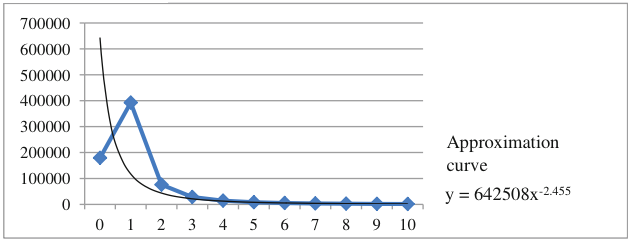
\includegraphics[width=0.55\linewidth]{charlieADegreeDistribution2}}
		\hfill
	}
	\caption{Degree distributions for the \textit{Charlie Hebdo} emotional case: (а) active users; (б) eliminated users. \textit{Source:} authors.}\label{fig:charlieADegreeDistribution}
\end{figure}

\begin{figure}[ht]
	\centerfloat{
		\hfill
		\subcaptionbox[List-of-Figures entry]{\label{fig:cologneDegreeDistribution-1}}{%
			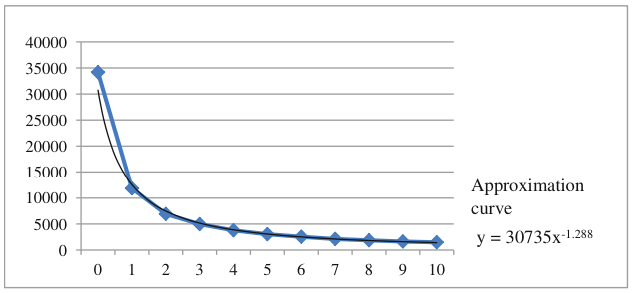
\includegraphics[width=0.51\linewidth]{cologneDegreeDistribution1}}
		\subcaptionbox{\label{fig:cologneDegreeDistribution-2}}{%
			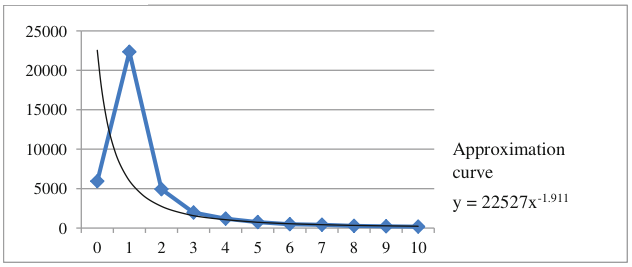
\includegraphics[width=0.55\linewidth]{cologneDegreeDistribution2}}
		\hfill
	}
	\caption{Degree distributions for the Cologne case: (а) active users; (б) eliminated users. \textit{Source:} authors.}\label{fig:cologneDegreeDistribution}
\end{figure}

\begin{figure}[ht]
	\centerfloat{
		\hfill
		\subcaptionbox[List-of-Figures entry]{\label{fig:berlinDegreeDistribution-1}}{%
			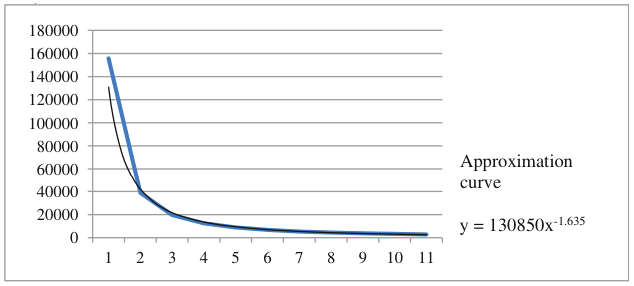
\includegraphics[width=0.51\linewidth]{berlinDegreeDistribution1}}
		\subcaptionbox{\label{fig:berlinDegreeDistribution-2}}{%
			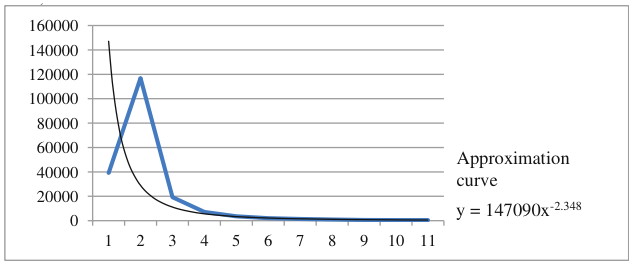
\includegraphics[width=0.55\linewidth]{berlinDegreeDistribution2}}
		\hfill
	}
	\caption{Degree distributions for the Berlin case: (а) active users; (б) eliminated users. \textit{Source:} authors.}\label{fig:berlinDegreeDistribution}
\end{figure}

\textit{H1.} All the cased that we have studied do, indeed, demonstrate power laws in degree distribution, and this is true for both active users (see Figs.~\cref{fig:biryuliovoDegreeDistribution-1},~\cref{fig:fergusonDegreeDistribution-1},~\cref{fig:charlieNDegreeDistribution-1},~\cref{fig:charlieADegreeDistribution-1},~\cref{fig:cologneDegreeDistribution-1} and~\cref{fig:berlinDegreeDistribution-1}) and eliminated users (see Figs.~\cref{fig:biryuliovoDegreeDistribution-2},~\cref{fig:fergusonDegreeDistribution-2},~\cref{fig:charlieNDegreeDistribution-2},~\cref{fig:charlieADegreeDistribution-2},~\cref{fig:cologneDegreeDistribution-2} and~\cref{fig:berlinDegreeDistribution-2}). Thus, power law is indicative for \textit{ad hoc} discussion outbursts across cultures and cases; H1 is supported.

\textit{H2.} All the cases do, indeed, diverge from the \(\lvert2.1\rvert\) expected exponent value to the same direction (see Table~\cref{tab:caseExponentValues}, column 2, exponent values for active users): the received exponent values are all equal or below 1.8, which indicates the lower power distance between the users. At the same time, the exponent values for eliminated users fluctuate around \(\lvert2.1\rvert\) to \(\lvert2.4\rvert\), the figures indicative for the Web degree distributions in various studies mentioned above. Thus, power laws with exponent values definitely below those discovered for the World Wide Web are indicative for \textit{ad hoc} discussions, which makes them, at least in terms of core vs. periphery relations, similar and comparable. The second part of the hypothesis is, though, not clearly supported: deviation from \(\lvert2.1\rvert\) substantially varies in percentage (from almost 40\% for the Cologne case to 14.3\% for \#jesuischarlie), and thus we cannot indicate any figure more precise than the fluctuation between \(\lvert1.28\rvert\) and \(\lvert1.80\rvert\) for ad hoc discussions; due to this, H2 is only partly proven. But we also need to state that, for three of six discussions, the exponent values were between \(\lvert1.56\rvert\) and \(\lvert1.63\rvert\), which corresponds to earlier results in \cite{WelchSchonfeldHe}.

\textit{H3.} For three of the six discussions (the Ferguson case and both Charlie Hebdo cases) the data were collected based on single hashtags (\#ferguson, \#charliehebdo, and \#jesuischarlie, respectively), while other cases were collected by keyword conglomerates ranging from 6 keywords (for the Biryuliovo case) to over a dozen keywords (for both German cases). As we see from Table~\cref{tab:caseExponentValues} and Figs.~\cref{fig:biryuliovoDegreeDistribution-1},~\cref{fig:fergusonDegreeDistribution-1},~\cref{fig:charlieNDegreeDistribution-1},~\cref{fig:charlieADegreeDistribution-1},~\cref{fig:cologneDegreeDistribution-1} and~\cref{fig:berlinDegreeDistribution-1}, there is no difference between single-hashtag and keyword-conglomerate data collection. H3 is supported, but this, paradoxically, might add not only to the evidence that \textit{ad hoc} discussions have similar patterns of degree distribution but also to the evidence that Twitter as a platform fosters the power law degree distributions in any type of discussion. To answer this, more research is needed.

\textit{H4.} As seen from Table~\cref{tab:caseExponentValues} and  Figs.~\cref{fig:biryuliovoDegreeDistribution-1},~\cref{fig:fergusonDegreeDistribution-1},~\cref{fig:charlieNDegreeDistribution-1},~\cref{fig:charlieADegreeDistribution-1},~\cref{fig:cologneDegreeDistribution-1} and~\cref{fig:berlinDegreeDistribution-1}, both neutral and affective hashtags are subjected to power law for both active and eliminated users, and exponent values deviate from \(\lvert2.1\rvert\) to the same direction. H4 is supported. We just need to mention that the compassion hashtag \#jesuischarlie has shown the highest exponent values, thus demonstrating bigger gaps between the influential and ‘peripheral’ users, and this might create room for further comparative investigations.

\paragraph{Discussion.} In search for proof of comparability of \textit{ad hoc} online discussions, we have applied our idea of evaluating degree distributions to six datasets of five comparable Twitter discussions on inter-ethnic conflicts in four countries that happened in the 2010 s. What we have discovered is the following.

First, we have shown that all the discussions we have observed are subjected to power law in degree distributions. Second, we have shown that exponent values for degree distributions in the discussion graphs diverge from the figures indicated for the Web on the whole in previous research. Moreover, they diverge in the same direction and to varying but, to a certain degree, also comparable percentage. Taken together, these findings indicate that, at least in terms of influence, interest, and/or power distribution in such discussions, they are comparable across countries and years, as well as across vocabulary types and neural/affective hashtags. Thus, exponent values may serve as indicators for the type of an online discussion. We have also shown that the peripheral part of the \textit{ad hoc} discussions was always closer to \(\lvert2.1\rvert\) to \(\lvert2.4\rvert\) exponent values discovered earlier for the Web and some social networks, which may be a sign that the \textit{ad hoc} discussions do differ from the ‘average’ network structure of the Web.

But we have also discovered that the exponent values for the discussions were fluctuating around \(\lvert1.6\rvert\) indicated earlier for Twitter on the whole; also, variance in value divergence from the expected figures was too big to state that a particular array of meanings may be indicative for ad hoc discussions and could become their structural marker. This needs further investigation, which might imply experimental design.

Last but not least, we have seen that \textit{ad hoc} discussions, if judged by the exponent values, show the patterns of lower power distance between core and periphery. This may be due exactly to their spontaneous nature, as institutional actors who shape and frame the offline discussions compete with ordinary users, crisis witnesses, and grassroots leaders. This may broaden our views upon discussion outbursts on social media.

\section{Тематическое моделирование контента}\label{sec:ch5/sect2}

\subsection{Topic modeling of conflict ad hoc discussions in social networks}\label{subsec:ch5/sec2/sub1}

\subsubsection{Introduction}

As a result of different media platforms achieving a steady user growth in a recent years more and more people begin to use different social networks as the main source of news on economical, political and social events. In particular, ad hoc discussions emerged which can be defined as a debate about a specific problem. In most cases such discussions appear in the case of controversial events and involve large number of participants.

Presence of such user activity raises the problem of analyzing large volumes of this type of data which has become one of the most important problems in many data analysis tasks, including topic modeling. Topic modeling algorithm in this case is an algorithm that, given the number of topics and the list of user messages can output two distributions: topics over documents and of words over topics. Such algorithm can help in the understanding of different points of view and highlight the main arguments. This can be useful in many ways one of which is the case in which the number of documents is big and we want to know their general content without reading them all. Another use case is data prepossessing, reducing the dimensions of data to use in other analysis tasks such semantic analysis. However directly applying traditional topic models like LDA and PLSA to short texts can be problematic primarily due to the sparsity of data given the specificity of short texts. In this paper we are studying the usage of different models on a large scale data which can effectively infer hidden topics in big discussions taking these features into account.

\subsubsection{Prior Work}

Early studies of the problem of topic modeling on short texts mainly concerned the use of external knowledge to improve the representation of text data. For example, Phan and others \cite{HoriguchiPhanNguyen} used the modeling of those short texts based on the traditional topic model, the effectiveness of which was tested on a large-scale data set for the purpose of short texts classification. In these works, it is assumed that the use of data derived from long texts could help improving the model for short texts. However, these methods are effective only when the auxiliary data are closely related to the original data. In the case of texts, obtained from social networks this task is impossible due to most of user messages being self-contained. Another assumption is based on the use of different aggregation methods. In the case of data, obtained from the Twitter, user messages can be aggregated by authors, publication time and hashtags. The \cite{WrayLexingRishabh} shows that the best performing method is based on hashtag based aggregation, however it can’t be applied then the texts themselves are collected using a series of hashtags (which is one of better ways for collecting data on big events). Author based aggregation can also be unreliable since the majority of users will have very few messages on any given topic. In this paper we are focusing on models, relying on statistical information about the data.

\subsubsection{Topic Models}

\paragraph{LDA.} Latent Dirichlet Allocation is a three-level hierarchical Bayesian model in which each element of the collection is modeled as a finite distribution over the set of topics. Each topic, in turn, is modeled as an infinite mixture by the set of topic probabilities \cite{MichaelJohnDavidAndrew}.

Lda assumes the following generative process:
\begin{itemize}
	\item Choose \(\theta_i \sim \textit{Dir}(\alpha)\)
	\item Choose \(\phi_i \sim \textit{Dir}(\beta)\)
	\item For every word position \(i, j\):
	\begin{itemize}
		\item Choose a topic \(z_{i, j} \sim \textit{Multinomial}(\theta_i)\)
		\item Choose a word \(w_{i, j} \sim \textit{Multinomial}({\phi_z}_{i,j})\)
	\end{itemize}
\end{itemize}
The model parameters \(\alpha\) and \(\beta\) are typically chosen sparse for better performance on short texts. In this paper, LDA is used as a baseline model, the effectiveness of which for standard texts has been proven both theoretically and in many experimental results.

\paragraph{BTM.} Biterm Topic Model performs topic modeling task by modeling a set of biterms (unordered word pair cooccurring in a short context). The main idea is that if two words co-occur more frequently, they are more likely to belong to a same topic \cite{YanyanJiafengXueqi}.

Btm assumes the following generative process:
\begin{itemize}
	\item Draw \(\theta_i \sim \textit{Dir}(\alpha)\)
	\item For each topic \(k\):
	\begin{itemize}
		\item draw \(\phi_k \sim \textit{Multinomial}(\beta)\)
	\end{itemize}
	\item For each biterm \(b_i\):
	\begin{itemize}
		\item draw \(z_i \sim \textit{Multinomial}(\theta)\)
		\item draw \(w_{i,1},w_{i,2} \sim \textit{Multinomial}({\phi_z}_i)\)
	\end{itemize}
\end{itemize}

As BTM does not model documents explicitly, we must provide a way to infer the topics in a document, i.e., evaluating the topic posterior. Using the chain rule the following equation was obtained:
\begin{equation}
	\label{eqn:29}
	P(z \mid b) = \sum P(z \mid b_i) P(b_i \mid d)
\end{equation}

Where \(P (z \mid b_i)\) can be obtained using via Bayes’ formula based on the parameters learned in BTM and \(P(b_i \mid d)\) can be calculated using empirical distribution of words in a document.

\paragraph{WNTM.} Word Network Topic Model’s idea is based on the following observations. When the texts are short, the word-document space is very sparse, but the word-word space still contains a large number of non-zero elements. Since the topic distribution for each doc- ument can not be recognized accurately in short or unbalanced texts, instead WNTM uses the topic distribution for each word \cite{KeYuanJichang}. Therefore, WNTM studies the distribution by topics for words, rather than those for documents. Studying the topics of the word, rather than those of the document make WNTM less sensitive to the length of the document. In addition, a network of words can be built with any type of text, which makes the WNTM model simple and universal in real applications, unlike other models, such as the mixture of unigrams \cite{ThrunMitchellNigam} and BTM.

The generative process of the model is in many respects similar to that of the LDA, but due to the use of a different distribution it has its own features:
\begin{itemize}
	\item For every latent word group \(z\) choose \(\phi \sim Dir(\beta)\)
	\item Choose \(\vartheta_i \sim \textit{Dir}(\alpha)\) distribution of a latent word group for adjacent word list \(L_i\) for word \(w_i\)
	\item For every word \(w_j \in L_i\):
	\begin{itemize}
		\item Choose a latent word group \(z_j \sim \vartheta_i\) 
		\item Choose an adjacent word \(w_j \sim {\phi_z}_j\)
	\end{itemize}
\end{itemize}

\begin{figure}[ht]
	\centerfloat{
		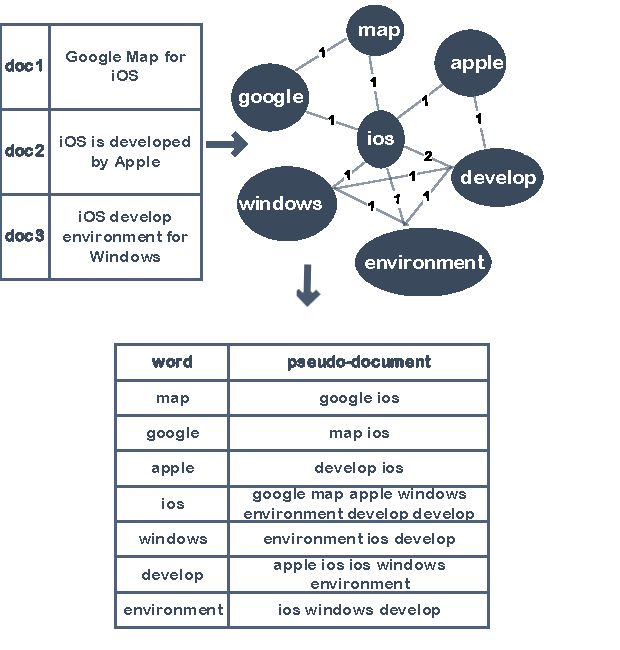
\includegraphics[scale=1.0]{wntmGeneration}
	}
	\caption{Generation of word network for WNTM model \cite{KeYuanJichang}.}\label{fig:wntmGeneration}
\end{figure}

Similarly to BTM this model can’t be directly applied to get topic distributions over documents. To get the topics in the document, we assume that the proportions of the words generated by the document is equal to the proportions of the document topics, that is:
\begin{equation}
	\label{eqn:30}
	P(z \mid d) = \sum P(z \mid w_i) P(w_i \mid d)
\end{equation}
Where \(P(z \mid w_i\)) equal \(\vartheta_{i,z}\), obtained in the generative process of WNTM and \(P(w_i \mid d)\) obtained as an empirical distribution of words in documents.

\subsubsection{Experiment}

The experiment was conducted to evaluate the quality of these three models, on three sets of ad hoc discussions. The following coherence measures were used to test the effectiveness of each model:

\begin{itemize}
	\item UMass \cite{MimnoWallachTalley} measures how often a common word of each topic is in average a good predictor for a less common word.
	\item NPMI \cite{StevesonAletras} is a normalized version of pointwise mutual information.
\end{itemize}

\paragraph{Data sets.} In this work models were tested on data, collected on three ad hoc discussions from Twitter social network: Riots in Biryulevo (Russia), October 2013 \cite{BodrunovaLitvinenkoBlekanov}, Ferguson unrest (USA), August 2014 \cite{SmoliarovaBlekanovBodrunova} Charlie Hebdo shooting (France), January 2015 \cite{SmoliarovaBlekanovLitvinenko}. The data was crawled based on hashtags in user messages.

\textit{Byrulevo. Riots in Biryulevo}
\begin{itemize}
	\item Total number of user messages: 10215
	\item Total number of users participated in the discussion: 11429
	\item Surveyed time period: 1.10.2013 - 31.10.2013
	\item Number of users who published tweets in the period under consideration: 3574
\end{itemize}

\textit{Ferguson. Ferguson unrest}
\begin{itemize}
	\item Total number of user messages: 193812
	\item Total number of users participated in the discussion: 169677
	\item Surveyed time period: 22.08.2014 - 31.08.2014
	\item Number of users who published tweets in the period under consideration: 70018
\end{itemize}

Charlie Hebdo. Charlie Hebdo shooting
\begin{itemize}
	\item Total number of user messages: 505069
	\item Total number of users participated in the discussion: 952615
	\item Surveyed time period: 07.01.2015 - 10.01.2015
	\item Number of users who published tweets in the period under consideration: 238491
\end{itemize}


\begin{table}[ht]%
	\centering
	\caption{Topics for Byrulevo data set.}%
	\label{tab:byrulevoTopics}% label всегда желательно идти после caption
	%	\begin{adjustbox}{width=1\textwidth}
		%		\small
		\begin{tabular}{ c  c  c  c }% Вертикальные полосы не используются принципиально, как и лишние горизонтальные (допускается по ГОСТ 2.105 пункт 4.4.5) % @{} позволяет прижиматься к краям
			\toprule
			Topic 1 & Topic 2 & Topic 3 & Topic 4 \\
			\hline
			\multicolumn{4}{c}{\makecell{LDA}} \\
			migrant & warehouse & broadcast & riot  \\
			Zeynalov & work & live & Manezhka \\
			police & man & moscow & moscow \\
			murder & boutique & photo & migrant \\
			Sherbakov & moscow & find & block \\
			\hline
			\multicolumn{4}{c}{\makecell{WNTM}} \\
			Moscow & news & Moscow & police \\
			event & Sherbakov & OMON & authorities \\
			Russia & migrant & Zeynalov & killer \\
			riot & murder & arrest & russian \\
			mayhem & killer & Sherbakov & meetings \\
			\hline
			\multicolumn{4}{c}{\makecell{BTM}} \\
			citizen & OMON & Sherbakov &  russian \\
			police & warehouse & Zeynalov & government \\
			local & police & killer & riot \\
			riot & arrest & arrest & migrant \\
			Moscow & killer & moscow & news \\
			\bottomrule
		\end{tabular}%
		%	\end{adjustbox}
\end{table}

\begin{table}[ht]%
	\centering
	\caption{Topics for Charlie Hebdo data set.}%
	\label{tab:charlieTopics}% label всегда желательно идти после caption
	%	\begin{adjustbox}{width=1\textwidth}
		%		\small
		\begin{tabular}{ c  c  c  c }% Вертикальные полосы не используются принципиально, как и лишние горизонтальные (допускается по ГОСТ 2.105 пункт 4.4.5) % @{} позволяет прижиматься к краям
			\toprule
			Topic 1 & Topic 2 & Topic 3 & Topic 4 \\
			\hline
			\multicolumn{4}{c}{\makecell{LDA}} \\
			policia & die & police & islam \\
			Paris & satire & shooting & religion \\
			terroristas & cartoonist & attack & youngest  \\
			sospechosos & frankreich & suspects & local \\
			ataque & attentater & update & extrimists \\
			\hline
			\multicolumn{4}{c}{\makecell{WNTM}} \\
			attack & suspects & cartoonists & media\\
			french & police & support & cartoons  \\
			today & two & editor & toxic \\
			terror & attack & respond & image \\
			killed & hostage & journalism & caricatures \\
			\hline
			\multicolumn{4}{c}{\makecell{BTM}} \\
			police & french & victims & muslims\\
			suspects & shooting & solidarity & islam \\
			hostage & gunman & attack & must \\
			killed & dead & France & say\\
			breaking & killed & jesuischarlie & religion \\
			\bottomrule
		\end{tabular}%
		%	\end{adjustbox}
\end{table}

\begin{table}[ht]%
	\centering
	\caption{Topics for Ferguson data set.}%
	\label{tab:fergusonTopics}% label всегда желательно идти после caption
	%	\begin{adjustbox}{width=1\textwidth}
		%		\small
		\begin{tabular}{ c  c  c  c }% Вертикальные полосы не используются принципиально, как и лишние горизонтальные (допускается по ГОСТ 2.105 пункт 4.4.5) % @{} позволяет прижиматься к краям
			\toprule
			Topic 1 & Topic 2 & Topic 3 & Topic 4 \\
			\hline
			\multicolumn{4}{c}{\makecell{LDA}} \\
			police & MikeBrown & militarization & Miami  \\
			life & black & police & overtown \\
			surrender & brown & law & America \\
			must & racism & reason & vote  \\
			dissa & justice & end & jail \\
			\hline
			\multicolumn{4}{c}{\makecell{WNTM}} \\
			MikeBrown & CNN & must & movement  \\
			amp & cops & surrender & speak \\
			police & Times & police & join  \\
			black & black & dissa & support \\
			people & shooting & see & now\\
			\hline
			\multicolumn{4}{c}{\makecell{BTM}} \\
			must & join & community & pd\\
			police & movement & Miami & look \\
			surrender & now & support & closer  \\
			dise & speak & lot & MikebBrown  \\
			click & die & overtown & msnbc \\
			\bottomrule
		\end{tabular}%
		%	\end{adjustbox}
\end{table}

\paragraph{Results.} Coherence measures were calculated and plotted to estimate the models’ effectiveness on different number of topics. The results (Figures~\cref{fig:charlieCoherence,fig:byrulevoCoherence,fig:fergusonCoherence}) allow us to talk about the approximate number of topics that is optimal for this task, but due to imperfection of quality indicators it requires manual clarification.

\begin{figure}[ht]
	\centerfloat{
		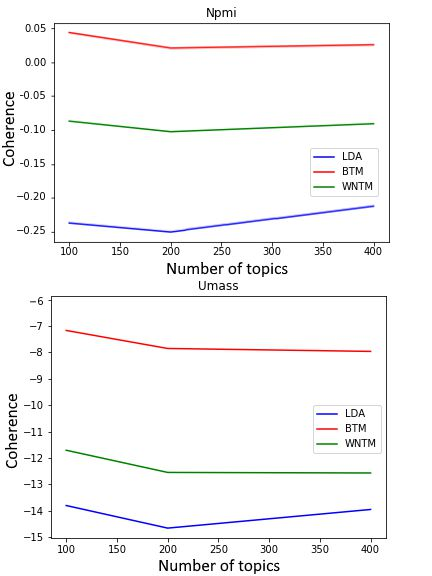
\includegraphics[scale=1.0]{charlieCoherence}
	}
	\caption{Coherence scores on Charlie Hebdo data set.}\label{fig:charlieCoherence}
\end{figure}

\begin{figure}[ht]
	\centerfloat{
		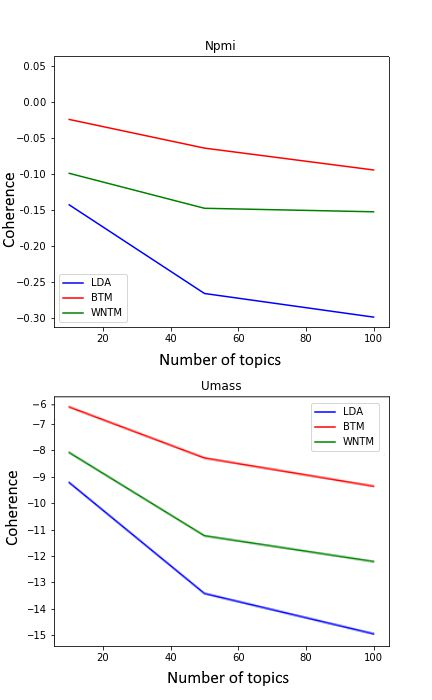
\includegraphics[scale=1.0]{byrulevoCoherence}
	}
	\caption{Coherence scores on Byrulevo data set.}\label{fig:byrulevoCoherence}
\end{figure}

\begin{figure}[ht]
	\centerfloat{
		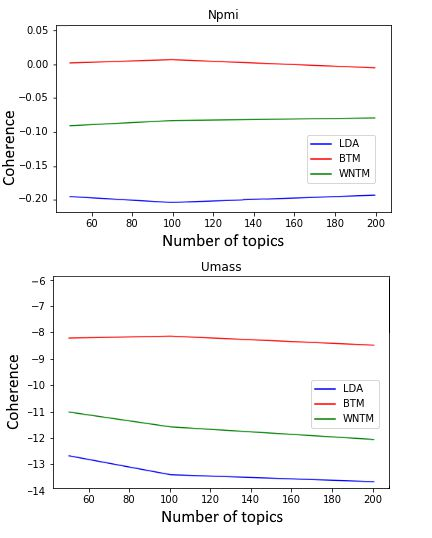
\includegraphics[scale=1.0]{fergusonCoherence}
	}
	\caption{Coherence scores on Ferguson data set.}\label{fig:fergusonCoherence}
\end{figure}

For each data set and topic model a few most coherent topics (topics focused on specific words which have the higher probability to occur in a specific topics) were chosen and can be seen in Tables~\cref{tab:byrulevoTopics,tab:charlieTopics,tab:fergusonTopics}.

As a result of the analysis of the given conflict ad hoc discussions, Biterm Topic Model came out to be the best performing and most stable method based on all coherence measures, baseline Lda model not specialized for working with short text has shown to not be suitable without the additional preprocessing of data mainly due to the data sparsity. However topics identified using this model can still be used to analyze key moments of discussions, participants’ arguments, and as a basis for other data analysis tasks.

Future work involves continuing the work on peer review, the first part of which was done for the Byrulevo data set by students and researchers from the journalism department of SPBU university. It has shown that the best results were obtained by the WNTM model. Comparing results of the models to the manual evaluation will allow us to measure not only the effectiveness of each model but also to compare coherence measures and find which one correlates better with human perception. The different prepocessing methods can also be used to improve the final result, tf-idf can be used instead of regular bag words approach to omit less frequent words more effectively.

\subsection{Topic detection based on sentence embeddings and agglomerative clustering with markov moment}\label{subsec:ch5/sec2/sub2}

\subsubsection{1. Introduction}

The task of finding topical or sentiment-based clusters in real-world textual datasets provides a wide range of methodological problems that are linked to both text clustering as finding the optimal number of clusters and text classification as assignment of a class to a text. The problem of topic detection has two arrays of problems intertwined: that of defining the optimal number of clusters and that of detecting similar texts, as the number of "real topics” depends on how many texts in a given dataset may be called similar enough \cite{NikolenkoKoltcovKoltsova}.

The ways of defining the topics may be divided into several major approaches. Of them, LSA- and LDA-based topic modelling goes “from clustering to classification”, by assigning texts to topic slots with probabilities that are based on the probabilistically measured word proximity \cite{Bodrunova2021}. Unlike traditional topic modelling, approaches as different as DBSCAN- and word2vec-based ones, go “from classification to clustering”, first measuring the word proximity and then defining clusters on this basis. But, for both ways, there are arbitrary parameters that need to be defined by the scholars, such as, e.g., the number of topics for LDA-based topic modelling or the two DBSCAN parameters that limit the number of possible clusters in advance. In “clustering-to-classification” thinking, the issue of optimal clustering is usually only partly resolved by multiple-run modelling with rounded number of clusters -- from 10 to 1000 or more \cite{GreeneCallaghanCunningham}. Additionally, LSA and LDA algorithms assume that all lexical units have equal weight within a dataset \cite{BleiNgJordan}, unlike in real sentences and texts, where nouns or verbs bear bigger semantic load, and some words are met much more frequently than others. To make models closer mirror the inequality of lexical units, various instruments of text pre-processing are employed that disambiguate between same-root words and eliminate stop words, rare words etc., as well as use more sophisticated models of pre-processing \cite{Bodrunova2021,SymeonidisEffrosynidisArampatzis}. DBSCAN-based approaches are widely used, but they are just as widely known for their low performance on data of high dimensionality, e.g., when the number of clusters goes over 10; for resolving this problem, a myriad of extensions have been proposed \cite{MittalGoyalHemanth}.

Thus, one needs to tackle two issues to unite the tasks of clustering and classification: the issue of word proximity estimation and the issue of finding the optimal number of clusters. They might be tackled simultaneously by constructing a methodology that combines decisions for both issues.

Below, we address both issues by testing the proposed clustering method on varying text representations and juxtapose the results with the known baselines. We propose a combination of Universal Sentence Encoder (USE) data pre-processing with sentence embeddings, agglomerative clustering by Ward’s method, and the Markov stopping moment. This method allows for uniting the assessment of text proximity with an optimal automated decision upon the number of clusters.

Earlier, we have conceptualized and theoretically modelled text clustering with hierarchic agglomerative methods with the Markov stopping moment for small datasets; the models showed positive results, while pre-processing was not yet a matter of our concern. We have also suggested their application to network-like representation of texts and sentiment analysis \cite{OrekhovKharlamovBodrunova,KharlamovOrekhovBodrunova}. In this paper, we test the proposed method of agglomerative clustering by Ward’s method with Markov stopping moment for several options of text representation, including more traditional tf-idf and improved word2vec and the sentence embeddings-based text representation. As quality metrics (in particular, V-measure) show, our method (Appendix A) stabilizes the result at the level of >0.5, the number of expected clusters being 10 and 20. Thus, the model performs much better than the existing baseline ones, including DBSCAN and OPTICS.

Raw data that are collected from social media provide additional challenges in terms of topic detection, due to their high noise, post length variations, author-induced grammar and lexicon distortions, and user-by-user dialogue fragmentation. The problem is especially significant for short user texts, like tweets \cite{BodrunovaBlekanovKukarkin}. Thus, before applying the model to data from social media for social science tasks, we used more structured real-world datasets for our experiment; these datasets had to be pre-labeled, as our goal was to test the method. To test our methodology, we have used the well-known real-world labeled dataset “20 newsgroups” (or, in short, News20) (http://qwone.com/~jason/20Newsgroups/) with pre-marked topicality. Four News20 subsets were used as the model text corpora, namely News3 (three classes and 83 documents), News5 (five classes and 121 documents), News10 (10 classes and 268 documents), and News20 (20 classes and 18,846 documents). We have also employed another real-world dataset, namely the BBC one (http://mlg.ucd.ie/datasets/bbc.html), with five thematic clusters \cite{GreeneCunningham}, to ensure that our results are dataset-independent.

For numerical experiments, we used a program code that was written in the Python 3.7 programming language. The NumPy and SciPy libraries were used for calculating distance matrices. The calculations were carried out using the PyCharm shell by JetBrains based on IntelliJ IDEA, and Collaboratory, a free environment for Google’s Jupiter Notebook.

The remainder of the paper is organized, as follows. Section 2 describes the methodological design, including data pre-processing with USE-based text representation, the approximation-estimation criterion and test, and the Markov stopping moment for finding the optimal number of clusters for the texts represented via embeddings. In Section 3, we report on the results as compared to the DBSCAN and OPTICS baselines by V-measure, NMI, and the number of clusters’ inference accuracy. In Discussion (Section 5) and Conclusion (Section 6), we re-assess the method and reflect upon its use on real-world data.

\subsubsection{2. Methods}

\paragraph{2.1. Data Pre-Processing with the Use Model}
In the “classification-to-clustering” logic, we have first represented the texts in a vector space. We have applied the Universal Sentence Encoder (USE) as a text pre-processing procedure to obtain high-quality contextual embeddings. USE is a transformer-based sentence encoding model that constructs sentence embeddings using the encoding sub-graph of the transformer architecture \cite{CerYangKong}. Transformer architecture consists of two main parts: an encoder and a decoder, where the latter outputs the final result in the form of a vector representation for a given sentence. USE utilizes the attention mechanisms to learn context-aware representations of words and, then, taking their ordering and identity, converts into a fixed-length sentence encoding vectors.

In our test, a pre-trained USE model is utilized in order to obtain sentence-level representations for the original data from the News20 dataset. The USE model was chosen due to several reasons. First, it is its efficiency in modeling small amounts of data, due to its nature as a pre-trained text model \cite{AharoniGoldberg}. Second, it is the quality it provides in general. Third, it is its quality of modelling on short or unbalanced texts then used as a pre-trained model. Fourth, there is a variety of pre-trained USE models that are suitable both for single-language and multilingual text corpora, which allows for economizing on computational resources.

\paragraph{2.2. Approximation-Estimation Test}
For the next step of our methodology, we rethink the classification problem as a more complex classification and clustering problem of automated typology of texts. In this case, both the topics of the documents and the number of these topics are unknown; they are not pre-defined by the supervisor. As stated above, a possible approach to the automated typology of texts could be unsupervised learning while using cluster analysis methods. For cluster analysis of texts, hierarchical agglomerative algorithms \cite{Everitt,DudaHartStork} can be used.

In general, strict cluster analysis (without intersecting clusters as subsets) is understood as algorithmic typologization of the elements of a certain set (sample) \(X\) by the “measure” of their similarity with each other. An arbitrary clustering algorithm is mapping

\begin{equation}
	\label{eqn:32}
	\mathcal{A}:
	\begin{cases}
		X \longrightarrow \mathbb{N},\\
		\overline{x_i} \longmapsto k,
	\end{cases}
\end{equation} which maps to any element \(\overline{x_i}\) from the set \(X\) the only \(k\), which is the number of the cluster to which \(\overline{x_i}\) belongs. The clustering process splits the \(X\) into pairwise disjoint subsets of \(X_h\) called clusters: \(X = \bigcup_{h = 1}^m X_h\), where for \(\forall h, l \mid 1 \le h, l \le m : X_h \cap X_l = \O\). Therefore, the map \(\mathcal{A}\) defines an equivalence relation on \(X\) \cite{Orekhov,Orekhov201811}. If an equivalence relation is given on some set X, not all set X can be considered, but only one element from each equivalence class. These elements are called “a representatives” of equivalence classes \cite{VanDerWaerden,Lang}. For cluster analysis, these are, for example, centroids or nearest neighbors. It greatly simplifies calculations and theoretical researchers of the map \(\mathcal{A}\).

One of the main problems when using agglomerative clustering methods is to calculate the preferred number of clusters and determine when the process stops. Moreover, a characteristic feature of these methods is the emergence of the so-called “chain effect” at the final stage of clustering. As we approach the end of the process, one large cluster is formed due to the addition of either previously created clusters or isolated points. If there is no criterion for stopping the clustering process, all points of the set \(X\) will be combined into a single cluster \cite{AldenderferBlashfield,Hartigan}.

The issue of defining the moment of completion of the clustering algorithm is the same moment that determines the optimal number of clusters. The problem of finding this moment can be solved within the framework of the theory of optimal stopping rules \cite{Wald,Sirjaev}.

Before proceeding to the formal mathematical calculations, we will explain the logic of the research design. Thus, we need to detect the optimal number of text types or classes (by topicality, sentiment, etc.) within a certain corpus and assign the types or classes to the texts. Formally, the number of classes (topics, in our case) will coincide with the number of clusters. An adequate number of clusters can be obtained if hierarchical agglomerative clustering stops at the “right moment”. Agglomerative clustering methods are based on combining the elements of some set \(X\) that are located closest to each other. Moreover, the agglomerative process begins with the assumption that each point in \(X\) is a separate cluster. During clustering, the clusters “grow” according to the principle described above. The clusters are clumps (subsets of higher density) inside \(X\). Obviously, with this approach, one of the main characteristics of the clustering process will be the function of minimum distances. While points close to each other are combined, the function of minimum distances slowly increases as a linear quantity. However, when the formed clusters begin to unite, the function of minimum distances increases sharply. In the vicinity of this point, the increase in the function of minimum distances ceases to be linear and becomes parabolic. By common sense, this is the moment of completion of the agglomerative clustering process. Analytically, this moment can be detected as a point at which an incomplete (without a linear term) parabolic approximation becomes more precise than the linear one.

In other words, in the neighborhood of this point, the quadratic error of incomplete parabolic approximation becomes smaller than the quadratic error of linear approximation. When clusters merge or one of the isolated points joins any of them, there should be a sharp jump in the minimum distance’s numerical value. It is the moment when the clustering process is complete. At such a moment, the values of the set of minimum distances are more accurately approximated by an incomplete quadratic parabola (without a linear term), rather than the direct line \cite{Orekhov,Orekhov201811}. Within this approach, the iteration of the agglomerative process of clustering, at which there is a change in the nature of the increase in the function of minimum distances from linear to parabolic, is defined as the Markov stopping moment.

We now turn to formal mathematical notation. Consider the set of minimum distances obtained
after \(m - 1\) iteration of any agglomerative clustering algorithm. It has the form \( \{F_1, F_2, \ldots, F_{m-1}\} \); for all of the agglomerative clustering methods, except for the centroid one, it is linearly ordered
relative to numerical values of its elements: \( 0 \le F_1 \le F_2 \le \ldots \le F_{m-1} \). We use this set to derive the statistical criterion for completing the clustering process in an arbitrary Euclidean space \(\mathbb{R}^n\).

We use the previously constructed parabolic approximation-estimation test in order to determine the moment when the character of a monotonic increase in the numerical sequence changes from linear
to parabolic \cite{Orekhov201809,Orekhov2018}.

We distinguish between a linear approximation in the class of functions of the form \(l(x) =
ax + b\) and an incomplete parabolic approximation (without a linear term) in the class of functions \(q(x) = cx^2 + d\). The quadratic errors in \(k\) nodes for linear and incomplete parabolic approximation will be, respectively, equal to:

\begin{equation}
	\label{eqn:33}
	\delta_l^2(k) = \sum_{i=0}^{k-1}(a \cdot i + b - y_i)^2; \quad \delta_q^2(k) = \sum_{i=0}^{k-1}(c \cdot i^2 + d - y_i)^2.
\end{equation}

If, in our reasoning, the number of approximation nodes is not essential or obvious from the context, then the corresponding quadratic errors will simply be denoted by \(\delta_l^2\), and \(\delta_q^2\).

When comparing \(\delta_l^2\), and \(\delta_q^2\), there are three possible cases: \(\delta_q^2 < \delta_l^2\); \(\delta_q^2 > \delta_l^2\); \(\delta_q^2 = \delta_l^2\).

We say that the sequence \(y_n\) has linear increase at the nodes (points): \(y_0, y_1, \ldots , y_{k-1}\), if \(y_n\) is monotonic and the quadratic errors of linear and incomplete parabolic approximation over these nodes are related by the inequality: \(\delta_q^2 > \delta_l^2\).

If, under the same conditions, the inequality: \(\delta_q^2 < \delta_l^2\), holds, then we say that the sequence \(y_n\) has parabolic increase at points: \(y_0, y_1, \ldots , y_{k-1}\).

If, for a set of approximation nodes: \(y_0, y_1, \ldots , y_{k-1}\), the equality \(\delta_q^2 = \delta_l^2\) holds, then the point \(y_{k-1}\) is called critical.

We calculate coefficients \(a,b\) of a linear function \(ax+b\) and the coefficients \(c,d\) for an incomplete quadratic function \(cx^2 + d\) approximating the nodes \(y_0, y_1, \ldots , y_{k-1}\) \cite{Orekhov201809,Orekhov2018}.

First, using the method of least squares, we calculate the coefficients \(a, b\) of the linear function \(f(x) = ax + b\) approximating the nodes \(y_0, y_1, \ldots , y_{k-1}\). For this, we find the local minimum of the
function of two variables

\begin{equation}
	\label{eqn:34}
	f_l (a, b) = \sum_{i=0}^{k-1}(a \cdot i + b - y_i)^2.
\end{equation} We calculate the partial derivatives of the function \(f_l (a, b)\):
\begin{equation}
	\label{eqn:35}
	\frac{\partial f_l}{\partial a} = 2a \sum_{i=0}^{k-1} i^2 + 2b \sum_{i=0}^{k-1}i - 2\sum_{i=0}^{k-1}i \cdot y_i;
\end{equation}
\begin{equation}
	\label{eqn:36}
	\frac{\partial f_l}{\partial b} = 2a \sum_{i=0}^{k-1} i + 2b \sum_{i=0}^{k-1}1 - 2\sum_{i=0}^{k-1} y_i;
\end{equation} By equating them to zero, we obtain a system of linear equations for the unknown \(a\) and \(b\):
\begin{equation}
	\label{eqn:37}
	\begin{cases}
		\frac{k(k-1)(2k-1)}{6} \cdot a + \frac{k(k-1)}{2} \cdot b = \sum_{i=1}^{k-1} i \cdot y_i \\
		\frac{k(k-1)}{2} \cdot a + k \cdot b = \sum_{i=1}^{k-1} y_i,
	\end{cases}
\end{equation} which implies:
\begin{equation}
	\label{eqn:38}
	a = \frac{6}{k(k^2 - 1)} {\sum_{i=1}^{k-1}(2i + 1 - k)y_i} \quad b = \frac{2}{k(k-1)} \sum_{i=1}^{k-1}(2k-1 - 3i)y_i.
\end{equation}

We calculate the coefficients \(c, d\) of the incomplete quadratic function \(cx^2 + d\) as the coordinates of
the local minimum for:

\begin{equation}
\label{eqn:39}
f_q(c, d) = \sum_{i=0}^{k-1} (c \cdot i^2 + d - y_i)^2.
\end{equation}


Differentiating \(f_q(c, d)\), we find:

\begin{equation}
	\label{eqn:40}
	\frac{\partial f_q}{\partial c} = 2c \sum_{i=0}^{k-1} i^4 + 2d \sum_{i=0}^{k-1}i^2 - 2\sum_{i=0}^{k-1}i^2 \cdot y_i,
\end{equation}
\begin{equation}
	\label{eqn:41}
	\frac{\partial f_q}{\partial d} = 2c \sum_{i=0}^{k-1} i^2 + 2d \sum_{i=0}^{k-1}1 - 2\sum_{i=0}^{k-1} y_i,
\end{equation} and
\begin{equation}
	\label{eqn:42}
		\begin{cases}
		\frac{k(k-1)(2k-1)(3k^2 - 3k - 1)}{30} \cdot c + \frac{k(k-1)(2k-1)}{6} \cdot d = \sum_{i=1}^{k-1} i^2 \cdot y_i \\
		\frac{k(k-1)(2k-1)}{6} \cdot c + k \cdot d = \sum_{i=1}^{k-1} y_i,
	\end{cases}
\end{equation}

We find that:
\begin{equation}
	\label{eqn:43}
	c = \frac{30}{k(k-1)(2k - 1)(8k^2 - 3k -11)}{\sum_{i=1}^{k-1}(6i^2 - (k-1)(2k -1))y_i};
\end{equation}
\begin{equation}
	\label{eqn:44}
	d = \frac{6}{k(8k^2 - 3k -11)}{\sum_{i=1}^{k-1}(3k(k-1) - 1 - 5i^2)y_i};
\end{equation}

Subsequently, to determine the moment when the character of the increase in the monotonic
sequence \(y_n\) changes from linear to parabolic, we construct the parabolic approximation-estimation
test \(\delta_{ql}^2\).

By definition, we assume that, for approximation nodes:  \(y_0, y_1, \ldots , y_{k-1}\) the parabolic
approximation-estimation test \cite{Orekhov201809,Orekhov2018} is expressed by the formula:

\begin{equation}
	\label{eqn:45}
	\delta^2 = \delta_{ql}^2(k) = \delta_l^2(k) - \delta_q^2(k).
\end{equation}

Moreover, we assume that always \(y_0 = 0\). It is easy to achieve this condition at any approximation step while susing the transformation:

\begin{equation}
	\label{eqn:46}
	y_0 = y_j - y_j, y_1 = y_{j+1} - y_j, \ldots, y_{k-1} = y_{j+k-1} - y_j.
\end{equation}

Now, we calculate, using the values of the coefficients \(a, b, c, d\), the quadratic errors of the linear and incomplete parabolic approximations at four points \(y_0, y_1, y_2, y_3\), and we obtain an explicit expression for \(\delta^2\)  \cite{Orekhov201809,Orekhov2018}.

\begin{equation}
	\label{eqn:47}
	\delta^2(4) = \delta_{ql}^2(k) = \delta_l^2(4) - \delta_q^2(4) = \frac{1}{245}(19y_1^2 - 11y_2^2 + 41y_3^2 + 12y_1y_2 - 64 y_1y_3 - 46y_2y_3).
\end{equation}

Thus, we have derived a quadratic form equal to the difference of the quadratic errors of linear and incomplete parabolic approximation. This quadratic form changes its sign when the character of an increase in the numerical sequence changes from linear to parabolic.

\paragraph{2.3. Cluster Analysis as a Random Process and the Markov Moment of Its Stopping}

Now, we will formally determine the moment of stopping the clustering process using the theory of random processes and the theory of sequential statistical analysis. Here, the approximation-estimation test is used as the decisive statistical criterion.

Let \(T = \overline{1, m - 1}\) be a bounded subset of the natural series, containing natural numbers: \(1, 2, \ldots, m - 1\). Subsequently, the family \(\xi = \{\xi_t, t \in T\}\) of random variables \(\xi_t = \xi_t(\omega)\) defined for \(\forall t \in T\) on the same probability space \((\Omega, \mathcal{F}, P)\) is called a discrete random process.

Each random variable \(\xi_t\) generates a \(\sigma\)-algebra, which we denote as \(\mathcal{F}_{\xi_t}\). Subsequently, the \(\sigma\)-algebra generated by the random process \(\xi = \{\xi_t,t \in T\}\) is called the minimal \(\sigma\)-algebra containing all \(\mathcal{F}_{\xi_t}\) i.e.,

\begin{equation}
	\label{eqn:48}
	\sigma(\xi) = \sigma(\bigcup_{t=1}^{m-1} \mathcal{F}_{\xi_t}).
\end{equation}

The discrete random process \(\xi = \{\xi_t, t \in T\}\) can be considered as a function of two variables \(\xi = \xi(t, \omega)\), where \(t\) is the natural argument, \(\omega\) is a random event. If we fix \(t\), then, as indicated above, we obtain a random variable \(\xi_t\); if we fix a random event \(\omega_0\), we obtain a function of the natural argument \(t\), which is called the trajectory of the random process \(\xi\) and is a random sequence of \(\xi_t(\omega_0)\).

We consider the clustering of a finite set \(X\) from the Euclidean space \(\mathbb{R}^n\) as a discrete random process \(\xi = \xi(t,\omega)\). A random event of \(\omega \in \Omega\) will be the extraction of a sample of \(X\) from \(\mathbb{R}^n\). Theoretically, any point \(\overline{x} \in \mathbb{R}^n\) can belong to the sample set \(X\), therefore the \(\sigma\)-algebra from the probability space \((\Omega, \mathcal{F}, P)\) contains all \(\mathbb{R}^n\), any finite set \(X\) from the space \(\mathbb{R}^n\), all possible countable unions of such sets, and additions to it. We denote this set system as \(\mathcal{S}(\mathbb{R}^n)\) and call it selective $\sigma$-algebra, \(\mathcal{F} = \mathcal{S}(\mathbb{R}^n)\). The same reasoning holds for any $\sigma$-algebra \(\mathcal{F}_{\xi_t}\) . Therefore, \(\sigma(\xi) = \mathcal{S}(\mathbb{R}^n)\).

Consider the binary problem of testing the statistical hypotheses \(H_0\) and \(H_1\). Where the null hypothesis \(H_0\), or the random sequence of \(\xi_t(\omega_0)\), increases linearly, and the alternative hypothesis \(H_1\), or the random sequence \(\xi_t(\omega_0)\), increases non-linearly (parabolically). It is necessary to construct the criterion as a strict mathematical rule that tests the statistical hypothesis.

In the Euclidean space, \(\mathbb{R}^n\) during agglomerative clustering of sample data, one of the main characteristics of the process will be a set of minimum distances. It is natural to consider its values as a random variable \(\xi_t : \Omega \longrightarrow \mathbb{R}\), assuming that t is the iteration number of the agglomerative clustering algorithm $\mathcal{A}$. For any fixed random event \(\omega_0 \in \Omega\), the corresponding trajectory \(\xi_t(\omega_0) = F_t\) is a monotonically increasing random sequence.

On the probability space \((\Omega, \mathcal{F}, P)\) the family of $\sigma$-algebras \(\mathfrak{F} = \{\mathcal{F}_t, t \in T\}\) is called a filtration, if for \(\forall i, j \in T \mid i < j: \mathcal{F}_i \subset \mathcal{F}_j \subset \mathcal{F}\). Moreover, if for \(\forall t \in T: \mathcal{F}_t = \sigma(\xi_i, i < t)\),then the filtration is called natural. The random process \(\xi = \{\xi_t, t \in T\}\) is called consistent with the filtration $\mathfrak{F}$, if for \(\forall t \in T :\sigma (\xi_t) = \mathcal{F}_{\xi_t} \subset \mathcal{F}_t\). Obviously, any random process is consistent with its natural filtration.

The mapping \(\tau: \Omega \longrightarrow T\) is called Markov moment with respect to the filtering $\mathfrak{F}$, if for \(\forall t \in T\) the preimage of the set is \(\{\tau \le t\} \in \mathcal{F}_t\). If, in addition, the probability \(P(\tau < +\infty) = 1\), then $\tau$ is called the Markov stopping time \cite{Sirjaev}.

In other words, let $\tau$ be the moment of the occurrence of some event in the random process \(\xi = \{\xi_t, t \in T\}\). If for \(\forall t_0 \in T\) we can definitely say whether the event $\tau$ occurred or not, provided that the values of \(\xi_t\) are only known in the past (to the left of \(t_0\)), then $\tau$ is the Markov moment relative to the natural filtering $\mathfrak{F}$ of the random process \(\xi = \{\xi_t, t \in T\}\). If the moment of the occurrence of $\tau$ has a probability equal to one, then $\tau$ is the Markov stopping time.

For a random sequence of minimum distances \(F_t\), when we cluster the sample \(X \subset \mathbb{R}^n\), the natural filtration consistent with the process is the “sample $\sigma$-algebra” \(\mathcal{S}(\mathbb{R}^n)\). Subsequently, by definition, the Markov moment of stopping the agglomerative process of clustering will be statistics

\begin{equation}
	\label{eqn:49}
	\tau = \min\{t \in T \mid \delta_t^2 > 0\}.
\end{equation}

Thus, the statistical criterion for the completion of the agglomerative process of clustering can be formulated, as follows. Let \(\{F_1, F_2,\ldots, F_k\}\) be a linearly ordered set of minimum distances, and the set \(\{y_1, y_2, \ldots, y_k\}\) be the “trend set” obtained using the transformation \(y_i = F_i + q \cdot i\), where \(q\) is the “trend coefficient”, and \(i\) is the iteration number of the agglomerative clustering algorithm \(\mathcal{A}\). The clustering process is considered to be completed at the \(k\)-th iteration, if for the nodes \(y_{k-4}, y_{k-3}, y_{k-2}, y_{k-1}\) the inequality \(\sigma^2 \le 0\), and for the set of points \(y_{k-3}, y_{k-2}, y_{k-1}, y_k\), the inequality \(\delta^2 > 0\).

In other words, the Markov moment of stopping the agglomerative clustering process is the minimum value \(t\) at which the null hypothesis \(H_0\) is rejected (“the values of the elements of a linearly ordered trend set increase linearly”) and the alternative hypothesis is accepted \(H_1\) (“the values of the elements of a linearly ordered trend set increase parabolically”) \cite{Orekhov}.

\paragraph{2.4. Clustering Stability and Determining the Preferred Number of Clusters: The Stopping Criterion}

The clustering process is completed using the parabolic approximation-estimation test described above, which estimates the jumps of a monotonically increasing sequence of “trend set” values. The magnitude of the significant jump sufficient to stop the process depends on the sensitivity of the stopping criterion, which is set using the non-negative coefficient \(q\) \cite{Orekhov,Orekhov201811}. The higher the value of \(q\), the lower the criterion’s sensitivity for stopping the clustering process. The stopping criterion has the highest sensitivity at \(q = 0\), in this case, as a result of clustering, the most significant number of clusters will be obtained. By increasing \(q\), the stopping criterion’s sensitivity can be reduced so that the process continues until all \(m\) vectors are combined into one cluster. In this case, intervals of stable clustering \(Q_i = [\alpha_i, \beta_i]\) will occur on which for \(\forall q \mid \alpha_i \le q \le \beta_i\) the same clustering results will be obtained.

Cluster analysis, in a sense, has a high degree of subjectivity. Therefore, the interpretation of its results largely depends on the researcher. So far, no rigorous definition of “sustainable/stable clustering” has been introduced; the scholars only speak of an intuitive concept. They argue that “clustering stability” shows how different the resulting partitions into equivalence classes become after using the clustering algorithms for the same data many times. A slight discrepancy between the results is interpreted as high stability \cite{GranichinShalymovAvros}.

In our case, a quantitative measure of stability of clustering can be considered the value of the interval of variation of the coefficient \(q\), within which the same result is obtained for the set \(X\). Here, we note again that the “chain effect” arises at the final stage of the clustering process when already-formed clusters are added one after another to some other cluster. In this case, the correct choice of sensitivity threshold for the stopping criterion on the account of the non-negative coefficient \(q\) is essential. In the general case, the sequence of intervals of stable clustering, for various values of the coefficient \(q\), is denoted by: \(Q_1, Q_2,\ldots, Q_{e-2}, Q_{e-1}, Q_e\),where \(Q_i (1\le i \le e - 1)\)is the interval of stable clustering, and \(Q_e\) is the set of values of the coefficient \(q\), in which all \(m\) points are combined into one cluster.

Clustering with Markov stopping time allows for automation of the procedure for determining the number of clusters in the text corpus. Based on the analysis of numerical experiments and general considerations, the following hypothesis was formulated earlier: “Preferred a number of clusters is formed at \(q \in Q_{e-2''}\) \cite{Orekhov201811}. The main motive for formulating this hypothesis was that a chain effect is manifested in the interval of stable clustering \(Q_{e-1}\), at which already formed clusters are combined.

\subsubsection{3. Comparison of the Proposed Approach with the Silhouette Score and the Elbow Method}

As stated above, to define the preferred number of clusters, we use the “e-2” hypothesis.

In detail, the “e-2” hypothesis works the following way. The coefficient of trend \(q\) increases monotonically, with some discreteness step from \(0\) to \(+\infty\). The first stable clustering interval is \(Q_1 = [0, a_1]\). For any \(q\) from \([0, a_1]\), the same clustering result is obtained, and the sample is divided into the largest number of clusters. These clusters are the smallest. The next stable clustering interval, \(Q_2 = [a_1, a_2]\), for any \(q\) from \([a1, a2]\), the same result is obtained again. Nevertheless, the number of clusters decreases, and the clusters become larger, etc. When the \(q\) trend coefficient increases, the preferred number of clusters is obtained. We denote this stable clustering interval \(Q_{e-2} = [a_{e-3}, a_{e-2}]\). It is clear that, for any \(q\) from \([a_{e-3}, a_{e-2}]\), the preferred number of clusters is obtained. On the interval of stable clustering \(Q_{e-1} = [a_{e-2}, a_{e-1}]\), a “chain effect” occurs, described in the literature on cluster analysis, for example \cite{AldenderferBlashfield}. In this interval of stable clustering, some of the already formed clusters merge. The coefficient \(q\) increases and reaches such a value ae that all sampling elements are combined into one cluster. We denote this ray of stable clustering by \(Q_e = [a_e, +\infty)\). From the text stated above, it is obvious that if the marked dataset contains less than three clusters, then the interval of stable clustering \(Q_{e-1} = [a_{e-2}, a_{e-1}]\) disappears. Therefore, for such datasets, the “e-2” hypothesis gives a bad result. Thus, it is clear that, for two-cluster datasets, use of the “e-2” hypothesis is not recommended, as the “e-1” step will be eliminated; however, for data with the presumed number of clusters being three or more, our method is capable of providing refined results. It needs to be underlined that the overwhelming majority of real-world datasets contain far more than two clusters: even in the simplest tasks of sentiment analysis, there are three clusters (negative, positive, and neutral), while, in topic detection, the number of clusters in large corpora is expected to be much bigger. Thus, our method is suitable for such datasets.

Below, we support this claim by applying our method first to the simplest standard model datasets from scikit-learn (https://scikit-learn.org/stable/modules/clustering.htmllibrary). The scikit-learn visualization of runs of clustering methods on six datasets of varying nature demonstrates that various clustering methods work differently on datasets with varying number of clusters (one, two, and three) and varying spreads of data units within the Euclidean space. The pictures at scikit-learn show that some methods work better on two-cluster datasets, and some do best on three-cluster ones.

Figure~\cref{fig:scikitLearnResults} shows the results of application of our method to the six model datasets.

\begin{figure}[ht]
	\centerfloat{
		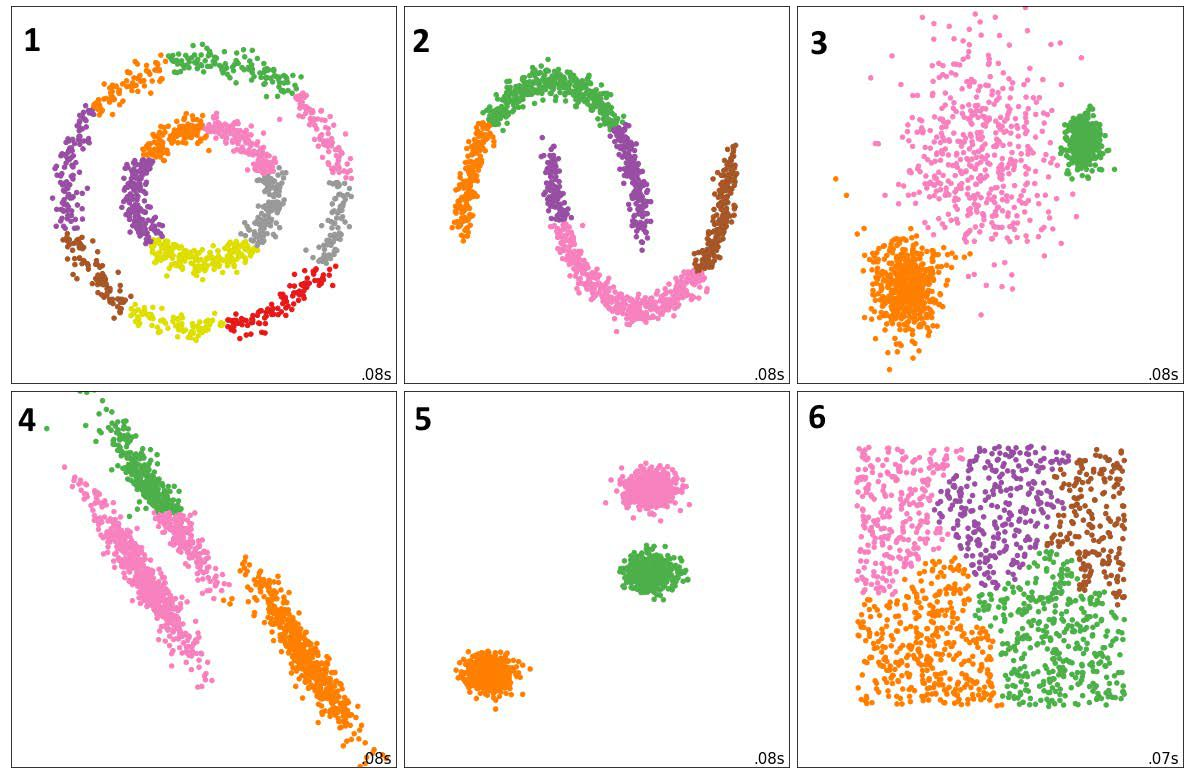
\includegraphics[scale=1.0]{scikitLearnResults}
	}
	\caption{Results of the proposed approach made on datasets from scikit-learn.}\label{fig:scikitLearnResults}
\end{figure}

Figure~\cref{fig:scikitLearnResults} allows for two conclusions. First, for three-cluster datasets, our method works well, the results are close to the Ward method, but work even better with borderline units (see visualizations for the datasets 3, 4, and 5, in comparison with the respective visualizations at scikit-learn for the Ward method). The visualization confirms that our method suits well for the datasets with three or more clusters. In this respect, the dataset 3 at Figure~\cref{fig:scikitLearnResults} deserves particular attention. This dataset contains three spherical clusters with fuzzy boundaries (compare to the dataset 5). Such distribution of points in a Euclidean space is typical for text representations by normalized vectors (e.g., embeddings-based representations). If we a priori assume that, according to the Euclidean metric, similar texts have similar vector representations, they should form spherical clusters. At the same time, the problem of fuzzy boundaries between different types of texts is well-known. According to Snell-Hornby \cite{SnellHornby}, there are no clear boundaries between types of texts, but only a certain center for each of the types. Therefore, we can assume that the representation of textual data by normalized vectors in the Euclidean space most closely matches the one of the dataset 3 at Figure~\cref{fig:scikitLearnResults}. Additionally, this is exactly where our method works best. Second, for the datasets with one or two clusters, our method detects a big number of clusters (see visualizations for the datasets 1, 2, and 6 at Figure~\cref{fig:scikitLearnResults}). This proves that use of the “e-2” hypothesis allows for catching the moment when the clustering process begins, before the chain effect shows up. Again, this proves that our method is suitable for datasets with large number of clusters, like the real-world ones used for topic detection.

Now, let us see how the “e-2” hypothesis works in comparison with more traditional ways of stopping to determine the preferred number of clusters, namely the silhouette metric and the elbow method. Our approach differs from both of them. The elbow method is a heuristic used to determine the number of clusters in a dataset. It consists of finding the “elbow” of the graph of change as a function of the number of clusters. The most common variation that is used in the elbow method is total variance within the cluster. The proposed method for determining the number of clusters using approximation-estimation tests is also based on finding the “elbow” of the graph of some values that characterize the clustering process. The difference is that the definition number of clusters with help of “elbow” is based upon heuristic visual assessment, but the definition number of clusters with help of approximation-estimation tests and “e-2” hypothesis is based upon sequential statistical analysis.

Unlike the elbow method, the silhouette coefficient is non-heuristic. It is based on two scores: \(a(x)\) is the average distance from current point \(x\) to objects of its own cluster \(A\), and \(b(x)\) is the average distance from the current point \(x\) to the objects of cluster \(B\), which is the closest one to \(x\). The silhouette coefficient of point \(x\) is the number \(s(x)\):


\begin{equation}
	\label{eqn:50}
	s(x) = \frac{b(x) - a(x)}{\max\{a(x), b(x)\}}.
\end{equation}

It is easy to see that \(-1 \le s(x) \le 1\). The value of \(s(x)\) being close to 1 implies that the point is clustered well; the value being close to \(-1\) implies that the point is clustered incorrect. If the value is close to 0, it it means that the distances from \(x\) to both clusters \(A\) and \(B\) are the same, and the point x should be assigned to either \(A\) or \(B\). This case can be considered as “ntermediate”. The silhouette coefficient of a dataset is defined as the average of the silhouette coefficients for all of the points of the sample. The number of clusters with the highest silhouette coefficient for the fixed clustering method can be determined as the optimal number of clusters for this method applied to the dataset under scrutiny \cite{Rousseeuw}.

However, the silhouette coefficient has its shortcomings. It takes much time to compute the silhouette coefficients for every data unit in large datasets for every possible clustering result. Additionally, the silhouette coefficient cannot detect well the original number of clusters if the clusters overlap and have fuzzy boundaries, while our method helps to eliminate this problem.

To prove it, we have applied our method to another well-known model dataset, namely the iris dataset (https://scikit-learn.org/stable/modules/generated/sklearn.datasets.load\_iris.html\#sklearn. datasets.load\_iris). The results of the application are shown in Tables~\cref{tab:irisSilhouetteCoefficient} and~\cref{tab:irisE2} (the silhouette coefficient and “e-2” hypothesis, respectively). The iris dataset consists of data of three classes, with two of them slightly overlapping, and our features for each data unit. Thus, the expected number of clusters is three. The results presented in Tables~\cref{tab:irisSilhouetteCoefficient} and~\cref{tab:irisE2} clearly show that the silhouette coefficient misses the point in detecting the right number of clusters, while our method finds the right number of clusters on the interval of stable clustering “e-2”.

\begin{table}[ht]%
	\centering
	\caption{The number of clusters received for the iris dataset by the silhouette coefficient.}%
	\label{tab:irisSilhouetteCoefficient}% label всегда желательно идти после caption
	%	\begin{adjustbox}{width=1\textwidth}
		%		\small
		\begin{tabular}{ c  c }% Вертикальные полосы не используются принципиально, как и лишние горизонтальные (допускается по ГОСТ 2.105 пункт 4.4.5) % @{} позволяет прижиматься к краям
			\toprule
			Number of Clusters & Silhouette Coeffecient\\
			\hline
			\textbf{2} & \textbf{0.6867} \\
			3 & 0.5543 \\
			4 & 0.4889 \\
			5 & 0.4843 \\
			6 & 0.3592 \\
			7 & 0.3422 \\
			8 & 0.3436 \\
			9 & 0.3305 \\
			10 & 0.2925 \\			
			\bottomrule
		\end{tabular}%
		%	\end{adjustbox}
\end{table}

\begin{table}[ht]%
	\centering
	\caption{The number of clusters received for the iris dataset by application of the e-2 hypothesis.}%
	\label{tab:irisE2}% label всегда желательно идти после caption
	%	\begin{adjustbox}{width=1\textwidth}
		%		\small
		\begin{tabular}{ c  c }% Вертикальные полосы не используются принципиально, как и лишние горизонтальные (допускается по ГОСТ 2.105 пункт 4.4.5) % @{} позволяет прижиматься к краям
			\toprule
			Number of Clusters & The Number of the Interval of Stable Clustering\\
			\hline
			1 & \(e\) \\
			2 & \(e - 1\) \\
			\textbf{3} & \textbf{\textit{e} - 2} \\
			8 & \(e - 3\) \\
			25 & \(e - 4\) \\
			144 & \(e - 5\) \\			
			145 & \(e - 6\) \\			
			\bottomrule
		\end{tabular}%
		%	\end{adjustbox}
\end{table}

\subsubsection{4. The Experiment against the Baselines and Its Results}

The tests were performed on two distinct datasets. News20 is a dataset containing news headlines and articles, which was split into four subsets. Each division contains rows with unique labels e.g., rows from a subset containing three classes is not used in subsets with five and 10 classes. BBC is a dataset containing BBC articles with each row labeled as one of the five distinct classes: sport, tech, business, entertainment, and politics.

The proposed model was tested against two other well-known clustering methods that have the ability to infer the optimal number of clusters as part of the training process. DBSCAN and OPTICS were chosen as one of the few classic approaches that does not require the number of clusters to train the model \cite{EsterKriegelSander,SchubertGertz}.

Three metrics were utilized to evaluate the performance of our method against classic approaches. The V-measure can be described as a weighted harmonic mean of homogeneity and completeness \cite{RosenbergHirschberg}. In this metric, the homogeneity criterion is satisfied if the algorithm only assigns to a single cluster the data units that are members of a single class. In order to satisfy the completeness criteria, the algorithm must assign to a single cluster all of the data units that are members of a single class. NMI (Normalized Mutual Information) \cite{StrehlGhosh} was used as additional performance metric, which utilises entropies of class labels and mutual information (a reduction in the entropy of class labels after training). Both of these metrics are independent of the absolute values of the labels, and the results of clustering can be directly compared with the true labels, which are document classes of the original data assigned by the authors of this dataset. Finally, to test models’ ability to accurately determine the number of clusters in a given corpus, we employed a measure of similarity between the optimal number of clusters and the number obtained by algorithms (number of clusters’ inference accuracy).

Experiments were conducted with different encoding techniques, in order to test their possible impact on the model’s performance. The first model is TF-IDF, as it is, to this day, a very popular encoding methods for relatively simple tasks. Another employed method is FastText \cite{BojanowskiGraveJoulin}, which is an extension of a well-known word2vec model with improved accuracy and faster training time due to the usage of negative sampling. Finally, we use the context-aware USE model described in Section 2, which, unlike FastText, can output embeddings not just for words but for entire sentences and, by doing so, bypasses the process of averaging the word embeddings typically performed by the models that do not utilise context information, such as FastText.

The results for different combinations of training and encoding models, as well as different metrics, can be seen in Tables~\cref{tab:vMeasure35}-\cref{tab:bbcDatasetResults}.

\begin{table}[ht]%
	\centering
	\caption{V-measure for News3 and News5.}%
	\label{tab:vMeasure35}% label всегда желательно идти после caption
	%	\begin{adjustbox}{width=1\textwidth}
		%		\small
		\begin{tabular}{ c  c  c  c  c  c  c }% Вертикальные полосы не используются принципиально, как и лишние горизонтальные (допускается по ГОСТ 2.105 пункт 4.4.5) % @{} позволяет прижиматься к краям
			\toprule
			 & \multicolumn{3}{c}{\makecell{News3}} & \multicolumn{3}{c}{\makecell{News5}}\\
			\hline
			Method & W2V & TF-IDF & USE & W2V & TF-IDF & USE \\
			\hline
			“e-2” hypothesis & 0.38 & 0.28 & \textbf{0.40} & 0.09 & 0.33 & \textbf{0.41} \\
			DBSCAN & 0.05 & 0.09 & 0.31 & 0.06 & 0.05 & 0.22 \\
			OPTICS & 0.20 & 0.26 & 0.24 & 0.08 & 0.16 & 0.11 \\
			\bottomrule
		\end{tabular}%
		%	\end{adjustbox}
\end{table}

\begin{table}[ht]%
	\centering
	\caption{V-measure for News10 and News20.}%
	\label{tab:vMeasure1020}% label всегда желательно идти после caption
	%	\begin{adjustbox}{width=1\textwidth}
		%		\small
		\begin{tabular}{ c  c  c  c  c  c  c }% Вертикальные полосы не используются принципиально, как и лишние горизонтальные (допускается по ГОСТ 2.105 пункт 4.4.5) % @{} позволяет прижиматься к краям
			\toprule
			& \multicolumn{3}{c}{\makecell{News3}} & \multicolumn{3}{c}{\makecell{News5}}\\
			\hline
			Method & W2V & TF-IDF & USE & W2V & TF-IDF & USE \\
			\hline
			“e-2” hypothesis & 0.09 & 0.13 & \textbf{0.64} & 0.08 & 0.22 & \textbf{0.52} \\
			DBSCAN & 0.01 & 0.24 & 0.38 & 0.02 & 0.18 & 0.09 \\
			OPTICS & 0.20 & 0.28 & 0.36 & 0.14 & 0.23 & 0.01 \\
			\bottomrule
		\end{tabular}%
		%	\end{adjustbox}
\end{table}

\begin{table}[ht]%
	\centering
	\caption{NMI for News3 and News5.}%
	\label{tab:nmi35}% label всегда желательно идти после caption
	%	\begin{adjustbox}{width=1\textwidth}
		%		\small
		\begin{tabular}{ c  c  c  c  c  c  c }% Вертикальные полосы не используются принципиально, как и лишние горизонтальные (допускается по ГОСТ 2.105 пункт 4.4.5) % @{} позволяет прижиматься к краям
			\toprule
			& \multicolumn{3}{c}{\makecell{News3}} & \multicolumn{3}{c}{\makecell{News5}}\\
			\hline
			Method & W2V & TF-IDF & USE & W2V & TF-IDF & USE \\
			\hline
			“e-2” hypothesis & 0.43 & 0.29 & \textbf{0.51} & 0.10 & \textbf{0.75} & \textbf{0.75} \\
			DBSCAN & 0.03 & 0.06 & 0.50 & 0.06 & 0.04 & 0.31 \\
			OPTICS & 0.19 & 0.31 & 0.26 & 0.06 & 0.19 & 0.11 \\
			\bottomrule
		\end{tabular}%
		%	\end{adjustbox}
\end{table}

\begin{table}[ht]%
	\centering
	\caption{NMI for News10 and News20.}%
	\label{tab:nmi1020}% label всегда желательно идти после caption
	%	\begin{adjustbox}{width=1\textwidth}
		%		\small
		\begin{tabular}{ c  c  c  c  c  c  c }% Вертикальные полосы не используются принципиально, как и лишние горизонтальные (допускается по ГОСТ 2.105 пункт 4.4.5) % @{} позволяет прижиматься к краям
			\toprule
			& \multicolumn{3}{c}{\makecell{News3}} & \multicolumn{3}{c}{\makecell{News5}}\\
			\hline
			Method & W2V & TF-IDF & USE & W2V & TF-IDF & USE \\
			\hline
			“e-2” hypothesis & 0.17 & 0.20 & \textbf{1.43} & 0.17 & 0.49 & \textbf{1.48} \\
			DBSCAN & 0.02 & 0.39 & 0.73 & 0.04 & 0.34 & 0.15 \\
			OPTICS & 0.30 & 0.47 & 0.70 & 0.24 & 0.46 & 0.01 \\
			\bottomrule
		\end{tabular}%
		%	\end{adjustbox}
\end{table}

\begin{table}[ht]%
	\centering
	\caption{The number of clusters’ inference accuracy for News3 and News5.}%
	\label{tab:clusterInfluence35}% label всегда желательно идти после caption
	%	\begin{adjustbox}{width=1\textwidth}
		%		\small
		\begin{tabular}{ c  c  c  c  c  c  c }% Вертикальные полосы не используются принципиально, как и лишние горизонтальные (допускается по ГОСТ 2.105 пункт 4.4.5) % @{} позволяет прижиматься к краям
			\toprule
			& \multicolumn{3}{c}{\makecell{News3}} & \multicolumn{3}{c}{\makecell{News5}}\\
			\hline
			Method & W2V & TF-IDF & USE & W2V & TF-IDF & USE \\
			\hline
			“e-2” hypothesis & 0.71 & \textbf{1} & 0.50 & 0.50 & 0.26 & 0.43 \\
			DBSCAN & \textbf{1} & \textbf{1} & 0.33 & 0.50 & 0.50 & 0.43  \\
			OPTICS & 0.20 & 0.14 & 0.14 & 0.78 & 0.25 & \textbf{0.82}\\
			\bottomrule
		\end{tabular}%
		%	\end{adjustbox}
\end{table}

\begin{table}[ht]%
	\centering
	\caption{The number of clusters’ inference accuracy for News10 and News20.}%
	\label{tab:clusterInfluence1020}% label всегда желательно идти после caption
	%	\begin{adjustbox}{width=1\textwidth}
		%		\small
		\begin{tabular}{ c  c  c  c  c  c  c }% Вертикальные полосы не используются принципиально, как и лишние горизонтальные (допускается по ГОСТ 2.105 пункт 4.4.5) % @{} позволяет прижиматься к краям
			\toprule
			& \multicolumn{3}{c}{\makecell{News3}} & \multicolumn{3}{c}{\makecell{News5}}\\
			\hline
			Method & W2V & TF-IDF & USE & W2V & TF-IDF & USE \\
			\hline
			“e-2” hypothesis & 0.14 & 0.08 & \textbf{1} & 0.20 & 0.14 & 0.84 \\
			DBSCAN & 0.33 & 0.33 & 0.38 & 0.33 & 0.78 & 0.51  \\
			OPTICS & 0.60 & 0.18 & 0.11 & 0.84 & 0.45 & \textbf{0.95} \\
			\bottomrule
		\end{tabular}%
		%	\end{adjustbox}
\end{table}

\begin{table}[ht]%
	\centering
	\caption{Results for BBC dataset (Universal Sentence Encoder (USE) data pre-processing).}%
	\label{tab:bbcDatasetResults}% label всегда желательно идти после caption
	%	\begin{adjustbox}{width=1\textwidth}
		%		\small
		\begin{tabular}{ c  c  c  c }% Вертикальные полосы не используются принципиально, как и лишние горизонтальные (допускается по ГОСТ 2.105 пункт 4.4.5) % @{} позволяет прижиматься к краям
			\toprule
			Method & V\_measure & NMI & The Number of Clusters’ Inference Accuracy \\
			\hline
			“e-2” hypothesis & \textbf{0.698} & \textbf{1.115} & \textbf{1} \\
			DBSCAN & 0.001 & 0.001 & 0.142 \\
			OPTICS & 0.166 & 0.216 & \textbf{0.816} \\
			\bottomrule
		\end{tabular}%
		%	\end{adjustbox}
\end{table}

The experiment shows that the proposed method of agglomerative clustering with USE pre-processing provides a much better result when compared to the baselineS, namely DBSCAN and OPTICS. The model performs especially well when the number of classes increases, reaching eight-times better performance than the baseline model if compared by the V-measure.

\subsubsection{5. Discussion}

As we have demonstrated above, the proposed method shows high efficiency against the baseline; however, it is not deprived of shortcomings.

As for data pre-processing and the dataset, the most notable downside to models, such as USE, are their requirements in terms of hardware and their time-consuming nature. This is especially true then the model is trained from scratch, but even the inference process can be rather slow then dealing with large corpora. Additionally, News20 has very well-defined classes and, as such, may not be representative of the performance on the real data. However, it provides a good enough estimate of the model performance by giving us the ability to check the clustering performance via comparing obtained cluster labels with the true labels defined for this set by human coding.

As for the clustering procedure with the Markov moment, it still possesses some residual subjectivity, as sensitivity of the stopping criterion may be changed by the researcher. As we noted above, clustering \textit{per se} is a subjective instrument when used for topicality or sentiment detection, as almost all of the stopping criteria (that is, the criteria for selection of the optimal number of clusters) are subjective by nature, being based on heuristic approaches to problem resolution. The use of “e-2 hypothesis” that we have suggested above aims at reducing the level of subjectivity. Additionally, more experiments are needed to collect empirical data on the optimal values of the stopping criterion for the real-world data. In order to overcome the problem of subjectivity, the data might as well undergo further experiments with various procedures for stopping, while the results might be compared to expert opinion, given that the level of agreement of 0.7-0.8 among the human coders is reached. However, we need to note that our prior experiments with topic models and human coding have shown that manual coding should not be taken as baseline. In particular, for pairs of human coders, topic interpretability and proximity varied for over 10 times, depending on prior familiarity with the dataset and coding experience \cite{BlekanovBodrunovaZhuravleva}. Thus, the quality assessment of clustering remains an issue. Our approach significantly helps researchers to reduce subjectivity but does not eliminate it completely. The advantage of our approach is that it allows for testing subtle changes in topicality distribution by nuanced variances of the stopping criterion, rather than changing the number of topic slots in arbitrary manner.

Possible limitations of our work may also lie in two aspects. The utilization of transformer-based sentence embeddings and USE may be advised to scholars interested in text clustering, but application of USE may be technically unfeasible for some of them. Additionally, the limitations might be linked to the nature of the datasets, which, as mentioned before, stands between regularized text collections and highly noisy data from social media.

\subsubsection{6. Conclusions}


Above, we have demonstrated the efficiency of a combined method for automated text typology that unites the tasks of text classification and text clustering. We have used sentence embeddings at the stage of pre-processing and hierarchical agglomerative clustering with an approximation-estimation test and the Markov stopping moment for defining the time of completion of clustering.

We have shown that this methodological design showed high efficiency in comparison with two baselines, DBSCAN and OPTICS. It is especially true for the number of clusters higher than five. The quality of the model does not drop at 10 and 20 classes, which allows overcoming the well-known problem of low performance of text classification for high numbers of clusters. The results may be applied to a wide array of tasks of text classification, including topic detection, multi-class sentiment analysis, and clustering of multilingual datasets by language. In combination with social network analysis, it may be applied for community detection on social networks and to other tasks of networked discussion analytics.

Real-world data can pose challenges to our method, as mentioned above. Thus, our future work will develop in three directions. First, we will apply the proposed method to the real-world datasets from unilingual and multilingual Twitter and Youtube that we have collected in 2014 to 2019 \cite{BodrunovaBlekanovSmoliarova}. We expect the results to drop to some extent, as the real-world data substantially complicate pre-processing. This is why, second, our future work will involve testing the model with other encoding methods such as XLNet, BERT, and others. Third, testing the model against other, more specialized clustering models and comparing them with the help of a wide array of metrics can also provide for better understanding of the efficiency of the model.

\subsection{The ideal topic: interdependence of topic interpretability and other quality features in topic modelling for short texts}\label{subsec:ch5/sec2/sub3}

\subsubsection{1. Introduction}

The studies of large text corpora via automated detection of topicality are a growing area of social research. Topic modelling is a probabilistic tool for discovering non-evident topics in a collection of texts. After the potential of topic modelling for Twitter has been proven \cite{RamageDumaisLiebling}, it has become a separate and growing area within topic detection research. Several works have shown that topic modelling of Twitter data is suitable for both detection of hidden discussion topics and data pre-processing aimed at reducing the topical dimensionality of the studied corpora \cite{BlekanovTarasovMaksimov,KoltsovaKoltcov}, as well as for a range of comparative tasks. In both capacities, it has already been applied to practical tasks like drug use analysis \cite{JonnagaddalaJueDai} or assessment of popular behavior during natural disasters \cite{LigutomOrioRamacho,MacedaLlovidoPalaoag}.

But, despite the promise, topic modelling is highly problematic when applied to short texts \cite{MazaruraDeWaalKanifer}, especially of the oral-written nature \cite{Lutovinova} often met online, of which Twitter is exemplary. Short texts, including Twitter posts (tweets), are today a popular form of public speech online, but their nature creates substantial obstacles to modelling topicality in Twitter corpora of virtually any size.

Topic modelling algorithms for the English language on Twitter have been explored widely, even if not extensively. Several models beyond LDA with Gibbs sampling, such as vector models or pLSA, as well as extensions for LDA, have been proposed. In most cases, classic unsupervised LDA performed worse than extended LDA or other models like biterm topic modelling (BTM). But, in some cases, LDA is used unquestioned, with results interpretable enough; this is why we will compare LDA which is in wide use with two other models described below.

Till today, comparative works on Twitter topic models for various languages beyond English remain very rare, mostly focusing on German and Spanish. Comparative studies of topic modelling for the francophone segment of Twitter are truly scarce, and, for the Russian-language Twitter, except for the earlier pilot works by our working group \cite{RamageDumaisLiebling,BlekanovTarasovMaksimov,SmoliarovaBodrunovaYakunin}, are almost non-extant. For a rare comparative work on five languages including French and Russian. This work, similar to ours in its goals, tests three models of topic detection, including the authors’ own development, and tests them by human coders and objective measures. The paper reports the comparative results on topic coherence and the so-called ‘utility’ of topic clusters (not topics!) without explaining how utility relates to human interpretability (whether this actually is interpretability or not). The authors also claim that their own model performs better than both LDA and BTM, but they do not reveal its full details for that would allow for comparison of the algorithms. Moreover, the results are not presented in full but, e.g. for all the languages beyond English, only on LDA and the authors’ model. Due to these reasons, we will look to French and Russian to once again compare the quality of topic detection.

Another gap in the current research on Twitter topics detection is that, except for e-health and natural disasters, issue- or event-oriented discussions are practically not studied. The methodological papers, including \cite{Sridhar}, do a lot to avoid limitations to overall Twitter topicality and work with large data that contain all possible topics. But, within a case-oriented discussion, detection of topics must be seriously complicated by the fact that the inner sub-topics share very similar lexicons.

To partly cover these gaps, we have taken under scrutiny three conflictual cases in three different countries, as they have provoked the respective Twitter discussion of a large scale but at the same time were focused enough for our experiment. In our earlier research, we have applied unsupervised LDA, as well as WNTM and BTM, to these three cases (see below), with BTM showing the best results by automated quality assessment metrics, namely Umass and NPMI \cite{BlekanovTarasovMaksimov}. But here we need to re-discuss our conclusions and juxtapose them to other, more subjective quality metrics such as topic saliency and human interpretation. Also, we try to see whether topic saliency and topic interpretability are linked to each other; to our best knowledge, this idea has not yet been explored by the academic community.

The remainder of the paper is organized as follows. In Sect. 2, we discuss the topic modelling algorithms that we use and the results we have received by applying the automated quality metrics and human coding, with the conclusion to reject both baselines. In Sect. 3, we present our ideas on the two other measures of topic detection quality, namely topic saliency and topic robustness. Section 4 serves for describing the cases and formulating the hypotheses. Section 5 provides the description of methods. In Sect. 6, we present the results and discuss them. To conclude, we formulate our idea of the ‘ideal topic’.

\subsubsection{2. Human and Automated Evaluation of Quality: Rejection of Both Baselines}

\paragraph{2.1 Automated Quality Assessment}

For automated quality assessment, we have used the coherence metrics that have gained popularity in the recent academic research, namely Umass and normalized PMI (NPMI). As we have shown in our earlier pre-tests, by both metrics, we have seen BTM to be performing better than the two other algorithms \cite{BlekanovTarasovMaksimov}.

But, after preliminary evaluation by human coders, we have seen that there are problems in topic interpretation that are not captured by the topic coherence metrics. Thus, the problems that we have discovered may be summarized as follows: 1) seemingly low number of interpretable topics; 2) a relatively big number of topics too similar to each other; 3) one-retweet-based topics gathered around one popular tweet rather than around a real topic in the discussion; 4) chained topics that unite several micro-themes but are non-clear to the human coders.

\paragraph{2.2 Human Coding and Its Artifacts}

Interpretability is understood here as an ability of a human coder to say why the topic descriptors (the most relevant words that describe the topic) stay together in a given topic. This is a traditional and ultimate metric of topic quality, as human interpretability is the ultimate goal of the whole modelling procedure. But this metric is non-feasible if the number of topics in multiple runs of the algorithms is overwhelming.

Interpretability is really hard to measure in an objective way. Moreover, below we show that human coding is critically dependent on three types of knowledge: that on the case, that on method, and that on the dataset. The difference in preparation to coding critically alters the coding results.

In Table~\cref{tab:coderTrainingArtifacts}, we show the coding results for three pairs of coders: unexperienced coders who have no detailed knowledge on the case, unexperienced coders who have received detailed instructions on the case and a lot of background knowledge, and members of our working group who have knowledge on the case, the dataset, and the algorithms.

\begin{table}[ht]%
	\centering
	\caption{Human coding of the Russian dataset, 100 topics: the artifacts of coder training.}%
	\label{tab:coderTrainingArtifacts}% label всегда желательно идти после caption
	%	\begin{adjustbox}{width=1\textwidth}
		%		\small
		\begin{tabular}{ c  c  c  c  c  c  c }% Вертикальные полосы не используются принципиально, как и лишние горизонтальные (допускается по ГОСТ 2.105 пункт 4.4.5) % @{} позволяет прижиматься к краям
			\toprule
			 & \multicolumn{2}{c}{\makecell{Unexperienced}} & \multicolumn{2}{c}{\makecell{Trained}} & \multicolumn{2}{c}{\makecell{Experienced}}\\
			\cline{2-7}
			& Coder 1 & Coder 2 & Coder 1 & Coder 2 & Coder 1 & Coder 2\\
			\hline
			LDA & 33\% & 11\% & 65\% & 94\% & 53\% & 63\% \\
			WNTM & 12\% & 11\% & 75\% & 92\% & 76\% & 73\%\\
			BTM & 22\% & 8\% & 88\% & 86\% & 76\% & 83\%\\
			\bottomrule
		\end{tabular}%
		%	\end{adjustbox}
\end{table}

As we see from Table~\cref{tab:coderTrainingArtifacts}, the coding result is, indeed, highly skewed by the coder background knowledge. Also, experienced coders from the working group show the tendency to give out a more balanced coding output, as they are more strict on the method performance and do not imply the inner grammar relations to the topics, filtering interpretability by the knowledge on the internal discourses in the dataset.

Thus, we see both automated dataset-level and human-based topic-level metrics to be unreliable in terms of finding ‘real topics’. This is why we suggest two other metrics and test their interconnectedness with human interpretability, to be able in future to substitute human coding by measuring these metrics.

\subsubsection{3. Topic-Level Quality Assessment: In Search of Independence Form Human Eye}

Thus, we have decided to introduce topic-level metrics of quality of topic modelling and test whether human interpretability will be related to them; we do it in an attempt to find topic-level metrics to substitute human coding without the necessity to assess the quality of the algorithm. At the same time, we still consider the well-known \textit{tf-idf} metric relevant for topic quality detection and will test our metrics against it in future.

\paragraph{3.1 Topic Saliency}

The idea of topic saliency lies in the fact that, for various time slots within a discussion, different sub-themes may emerge as the leading ones. Saliency is calculated in the following way. Each document in the dataset is assigned a topic distribution; then, based on the time of publication, the topic distributions in the tweets are summarized, and, for each topic, the saliency is calculated as the sum of the tweets belonging (with a certain probability) to the particular topic. Since the intensity of the discussion may vary in time, the overall topic saliency for all topics may vary (from 0 to 1, in our case). We have used a 24-h step and measured the topic saliency for each day in aggregate. This strategy constitutes one of the limitations for our study, as the French dataset encompasses four days only, due to its overwhelming volume (see below); in future, for the 4-day French dataset, we plan to change the step and conduct an hourly analysis.

To our best knowledge, topic saliency has not yet been discussed in the literature as a possible quality metric for topic modelling. But, by commonsense logic, topic saliency should be related to topic interpretability: the more salient a topic is, the bigger it is within the dataset and must be easier to interpret. And, if so, topic saliency may in future be seen a quality metric -- a proxy for understanding topics by human coders.

\paragraph{3.2 Topic Robustness}

Topic robustness shows whether the topic is composed of a relatively large number of relevant texts/words. We will look at the relevance levels of topic descriptors (top words). The relevance is, basically, the extent to which a particular word belongs to a given topic, depending on how many times it is met in the topic-relevant tweets; the relevance is measured 0 to 1. There is no clear agreement in today’s research what relevance is to be considered high; this metric is dataset-dependent and thus needs to be assessed for each topic depending on the highest levels for a given run of topic modelling. Usual values for word relevance range from 0.01 to 0.1 for short-text small datasets to 0.001 to 0.05 for longer-text larger datasets.

Topic robustness, thus, combines two internal parameters: the word relevance to a topic and the number of relevant words in a topic. Robust topics are those who have many highly relevant words; it means they attract a lot of similar texts. We will provide the exact measurements for topic robustness in Sect. 5. But topics with lower robustness must not be viewed as ‘bad’: robustness highly depends on the nature of the discussion.
We will check the relationships between these metrics, to see how one can describe an ideal topic: a robust, understandable, salient one -- and assess which datasets (bigger/smaller, monolingual/multilingual) provide for a bigger quantity of ideal topics.

\paragraph{4. The Cases Under Scrutiny and the Research Hypotheses}

Here, we describe the cases we work with, which will help formulate the hypotheses. For this research, we work with the datasets from Twitter on the three cases:

\begin{itemize}
	\item Anti-immigrant riots in the Moscow district of Biryulevo, Russia, 2013: number of users who published tweets -- 3574, total number of user messages -- 10215;
	\item The Ferguson unrest, USA, 2014: number of users who published tweets -- 70018, total number of messages -- 193812;
	\item The Charlie Hebdo shooting, France, 2015: number of users who published tweets -- 238491, total number of messages -- 505069.
\end{itemize}

The datasets are highly uneven in volume, and thus we had conducted pre-tests of the number of topics that would provide the most interpretable results and, at the same time, remain comparable. We ran the topic modelling for all the three cases with the BTM algorithm for the following number of topics set arbitrarily: for Biryulevo, 10, 50, and 100; for Ferguson, 50, 100, and 200; for Charlie Hebdo, 100, 200, and 400 topics. We have pre-tested their interpretability for small numbers of topics for each run (10 to 20), and we have seen that, for 100 topics, the results may be comparable. This is why we will further on use the 100-topic runs for comparing the quality assessment results.

Having in mind the aforementioned metrics for quality assessment and the number of topics in each run, we have set the following hypotheses:
\begin{itemize}
	\item H1. Human-based interpretability will correspond to the volume of the dataset: the bigger the dataset, the more interpretable the topics are.
	\item H2. Human-based interpretability will be higher for monolingual discussions (Russia, the USA) than for multilingual discussions (France).
	\item H3. More interpretable topics will have higher saliency in all the datasets. 
	\item H4. More interpretable topics will show higher robustness in all the datasets. 
	\item H5. More robust topics will have higher saliency in all the datasets.
\end{itemize}

We note that H1 and H2 are mutually exclusive.

\subsubsection{5. The Research Methods}

Here, we will in short describe the methods we use to test the hypotheses. As tour data collection has been well-described in our previous works, we will only provide the description for the methods directly used in this paper.

For H1 and H2, we have worked with native speakers as human coders. Unlike in other research, we do not test the inter-rater reliability for the coders and then let them code separate segments of the task. Instead, two coders were asked to code the topic descriptors independently, and then, their inter-coder reliability was checked. We used this to see how divergent the opinions of the coders could be and whether the number of interpretable topics corresponds to earlier studies of longer texts, e.g. Russian blogs \cite{KoltsovaKoltcov}. Thus, six coders were instructed to code the topics as interpretable or non-interpretable based on the abovestated assumption of comprehensibility of why the topic descriptors stay together in a particular topic. Then, the number of interpretable topics for each coder and the meta-coding results were calculated. Each topic was assigned an interpretability index of 0 (non-interpretable for both coders), 1 (interpretable for one coder), or 2 (interpretable for both coders).

In case of France, multi-lingual coders had to work (those who could recognize English, French, Spanish, Italian, German, and, with additional help, Russian). Finding such coders constitutes a separate problem in assessing the quality of multilingual global- scale discussions. We consider the procedures of assignment of meaning comparable for Russia, the USA, and France, as interpreting the topic descriptors requires simple word recognition procedures and basic knowledge of language(s), which makes recognition of a top word the unit of interpretation, disregarding the language belonging of a word.

For H3, topic saliency was automatically calculated based on the modelling results, and the saliency thresholds were defined based on the overall saliency picture for a given case. But, as the saliency measurements have shown, topics could be considered salient if they reached circa 30\% of the overall saliency of topics in a given day. Then each topic was assigned a saliency index of 0 (the topic has never reached over 30\% of the overall saliency for a particular time slot), 1 (the topic has at least once reached over 50\% of saliency for a particular time slot), or 2 (the topic stably reached over 50\% of saliency in at least 30\% of the overall time span for the case). Then, Spearman’s rho was used to see the dependencies between topic interpretability and topic saliency.

For H4 and H5, we have calculated the topic robustness for each topic. First, we have calculated the word relevance and have established 0.02 as the high relevance threshold. Then, we have introduced the robustness score: if a topic has no top words with the relevance reaching 0.02, it is non-robust (0); if there are up to 5 words of the relevance of 0.02 or higher, the topic is acceptably robust (1); if there are more than 5 words with the relevance of 0.02 or higher, the topic is fully robust (2).

\subsubsection{6. Results and Discussion}

\textit{H1.} We have presupposed that the datasets with a bigger amount of tweets will provide for better topic extraction, if the number of topics is the same. But H1 has to be rejected, as we have found that the number of highly interpretable topics was almost the same for all the datasets: 45 of 99, for Russia; 40 of 96, for the USA; and 41 of 100, for France (topics on non-Russian and non-English were eliminated from the first two cases). Thus, we do not observe any growth of interpretability for bigger tweet collections.

\textit{H2.} The same goes for H2: we do not observe higher interpretability for monolingual cases, given that the coders understand the languages of the multilingual discussion.

Rejection of H1 and H2 is telling, as it provides input for understanding the nature of topic interpretability on Twitter using BTM. Only circa 40--45\% of the topics get surely interpreted, which needs to be addressed in the future research. In the French case, most non-interpretable topics were composed by tweets in different languages, first and foremost French, English, and Spanish. The algorithm that puts the tweets in different languages into one topic is still to be analysed, to prevent the mixing of languages in future. Another problem discovered both in the ‘international’ topics and in the francophone one is the over-abundance of pronouns, service words and particles as top words. In the biterm-based approaches, eliminating them from the pre-processed dataset would significantly change the clustering results; but maybe a decision here is simple -- they should not be allowed to the lists of topic descriptors, thus leaving more space to the meaningful top words.

\textit{H3--H5.} For the results for H3 to H5, see Table~\cref{tab:topicQualityMetrics}.

\begin{table}[ht]%
	\centering
	\caption{Human coding of the Russian dataset, 100 topics: the artifacts of coder training.}%
	\label{tab:topicQualityMetrics}% label всегда желательно идти после caption
		\begin{adjustbox}{width=1\textwidth}
				\small
		\begin{tabular}{ c  c  c  c  c  c  c  c  c  c }% Вертикальные полосы не используются принципиально, как и лишние горизонтальные (допускается по ГОСТ 2.105 пункт 4.4.5) % @{} позволяет прижиматься к краям
			\toprule
			& \multicolumn{3}{c}{\makecell{Russia}} & \multicolumn{3}{c}{\makecell{The USA}} & \multicolumn{3}{c}{\makecell{France}}\\
			\cline{2-10}
			& Interpr. & Saliency & Rob. & Interpr. & Saliency & Rob. & Interpr. & Saliency & Rob. \\
			\hline
			Interpretability & -- & \(-0,080\) & 0,064 & -- & 0,226* & 0,192 & -- & 0,337*** & 0,396*** \\
			Saliency & \(-0,080\) & -- & 0,261** & 0,226* & -- & \(-0,086\) & 0,337*** & -- & 0,345*** \\
			Robustness & 0,064 & 0,261** & -- & 0,192 & \(-0,086\) & -- & 0,396*** & 0,345*** & -- \\
			\bottomrule
			\multicolumn{10}{@{}p{\textwidth}}{%
%				\vspace*{-4ex}% этим подтягиваем повыше
				\hspace*{2.5em}% абзацный отступ - требование ГОСТ 2.105
				Note. * -- \(p \le 0,05\); ** -- \(p \le 0,01\); *** -- \(p \le 0,001\).
			}\\
		\end{tabular}%
			\end{adjustbox}
\end{table}

Table~\cref{tab:topicQualityMetrics} does not provide for any systematic picture of the interdependence of the three topic quality metrics. Our hypotheses were formulated the way that they demanded a clear picture, which is not always the case in practice. In the way they are formulated, they have to be rejected; but important conclusions can be drawn.

Thus, more interpretable topics are more salient in the US and French cases. This might have to do with the dataset volume. And the French case, despite its multilingualism, shows that the three aspects of the topic detection quality may be interdependent.

The correlations for the French case are stronger than for the monolingual cases, and this definitely demands future research on how multilingual discussions are constructed in terms of topicality and why the multilingual discussions perform better than monolingual ones, which is quite counter-intuitive.

To conclude, we underline the following. Putting our results against previous research, we need to state that interpretability for Twitter is significantly lower than for longer-text datasets (cf. \cite{KoltsovaKoltcov}). Also, looking at topic/dataset characteristics like robustness and saliency may provide for better understanding of the nature of an ideal topic. In all 300 topics we have assessed, only 7 were all robust, salient, and well-interpretable.

\subsection{Topics in the Russian Twitter and relations between their interpretability and sentiment}\label{subsec:ch5/sec2/sub4}

\subsubsection{1. Introduction}

After the principal possibility of topic modelling on such short and noisy texts as tweets has been demonstrated over ten years ago \cite{RamageDumaisLiebling}, it has become a focus of scholarly attention as a method of detection of hidden substance of the tweet corpora, tracking user behavior, and pre-processing to reducing the dimensionality of the corpora. For English, an extensive number of studies have been made, and several algorithms have been proposed. For other languages, though, there have been much fewer experiments, especially of comparative thought.

Despite, by the nature of topic modelling, short and noisy natural-language texts are virtually the worst object for topic detection, and despite the diminishing relevance of Twitter in the media ecosystems of many countries, the attractiveness of Twitter as a source of datasets for modelling remains high -- again, mostly for the English-language cases.

Russian social media have so far received moderate attention in terms of experiments with topic modelling, and the Russian Twitter has not been its primary focus. In particular, topic interpretability has not received, to our viewpoint, enough scholarly attention. Despite topic quality is quite an expansive research area (for a review, see \cite{MavrinFilchenkovKoltcov}), only several studies have addressed the divergence between the objective and subjective topic quality assessment, especially rarely for Russian \cite{BodrunovaKoltcovKoltsova}. The causes of low interpretability of topics for short texts have virtually escaped proper discussion, and no studies have been dedicated to linking topic semantics and their interpretability.

Our work aims at partly covering the gaps described above. We model the topics for a dataset of a conflictual discussion of as early as 2013, as at that moment, according to our previous studies \cite{BodrunovaLitvinenkoBlekanov2017}, the Russian Twitter was not as bot-occupied as it has been since 2016 \cite{StukalSanovichBonneau}. We have chosen to work with conflicts online, as they provide for emotionally loaded texts and link the discussions to a variety of wider issues of user interest.

Earlier, we have tested three topic modelling algorithms, namely unsupervised LDA, BTM, and WNTM, on three raw-data Twitter datasets in English, French, and Russian, including the aforementioned dataset \cite{BlekanovTarasovMaksimov}. But, as it often happens in topic modelling studies, the results must be tested also by human coders. Below, we will describe in short what and why we have done in terms of algorithm development and what we have tested additionally to provide more freedom to human coders.

The remainder of the paper is organized as follows. In Section 2, we review the literature on topic modelling and Twitter studies in Russia and beyond. In Section 3, we formulate the hypotheses, tell of the case under scrutiny, our previous topic modelling experience with the three algorithms, and suggest data amplification for human coders. In Section 4, we describe the method and the research procedures. Section 5 provides the results and discusses them for both the process of human coding and the results based on sentiment analysis. The concluding remarks reformulate our findings against prior knowledge and provide the guidelines for further research.

\subsubsection{2. Topic Modelling for Russian Social Media: A Literature Review}

To our best knowledge, there has so far been no extensive review of how topic modeling has developed for the Russian language. Not aspiring for a truly representative one, we anyway need to review the field to show how scarce attention has so far been given to the relations between the interpretability of modelling results and the topics’ inherent features. This, at least partly, is also true for topic modelling studies for other languages.

For Russian, topic modelling studies may be divided into methodological (that develop, compare, and extend models as well as evaluate their quality), applied (that apply topic modelling to extract the meanings from datasets), and relational (that relate topic modelling results to other features of the datasets or external factors).

\paragraph{A. Methodological studies of topic modelling} 
There are several groups within Russia who have been focusing on various topic modelling algorithms. Thus, in a sequence of influential works, Koltsova and colleagues develop LDA \cite{KoltcovKoltsovaNikolenko2014} and a range of extensions to it. The latter include semi-supervised interval LDA, or ISLDA \cite{BodrunovaKoltcovKoltsova}, granulated LDA \cite{KoltcovNikolenkoKoltsova0516} and LDA with local density regularization \cite{KoltcovNikolenkoKoltsova0916}. In relation to this work, Koltsov and colleagues have optimized Gibbs sampling \cite{KoltcovNikolenkoKoltsova16} and the model itself applying Rényi and Tsallis entropies \cite{Koltcov}. This group of authors has linked the use of topic modelling to qualitative studies of social media and beyond \cite{NikolenkoKoltcovKoltsova} and applied their instruments to several corpora of longer and shorter texts (see below). In these works, Russian is used more as an example of ‘a language as such’, just as English is used in topic modeling, often without discussing inherent linguistic or contextual limitations. Similarly, the works by Vorontsov and colleagues (e.g. \cite{VorontsovFreiApishev1015,VorontsovPotapenko,VorontsovFreiApishev0415}) have been influential in pLSA and its modifications based on non- Bayesian regularization. Among the rest, they have tested two algorithms for the Russian-language short texts, namely biterm topic modelling (BTM) and word network topic model (WNTM) \cite[p.~191]{KochedykovApishevGolitsyn} which we have also employed for our Twitter study (see \cite{BlekanovTarasovMaksimov} and below). The two research groups have collaborated on additive topic models \cite{ApishevKoltcovKoltsova1016,ApishevKoltcovKoltsova16} and have published important methodological papers in Russian (which we do not review here due to the scarcity of space). We will also omit from our review the works that suggest text clustering instruments alternative to topic modelling.

Several other authors have amplified this corpus of works by adding automated labeling to Russian-language topics \cite{MirzagitovaMitrofanova}, showing the possibility of single term extraction by topic modelling \cite{BolshakovaLoukachevitchNokel}, and multi-model tests on optimization of the number of topics \cite{KrasnovSen}.

\paragraph{B. Use of topic modelling for content interpretation: applied and relational works}
Content-exploring research has scrutinized both social media and text corpora beyond them. Thus, topic modelling has been employed to map the agenda of the Russian Livejournal of 2013 \cite{KoltsovaKoltcov} and ethnic contents of the Russian blogs \cite{Nagornyy}, including detection of most hated ethnicities \cite{BodrunovaKoltsovaKoltcov}.

Beyond the social networking realm, LDA has been applied to TV topics \cite{KoltsovaPashakhin}, Russian prose \cite{SedovaMitrofanova}, a corpus of musicological texts \cite{Mitrofanova}, newspaper news texts on climate change \cite{BoussalisCoanPoberezhskaya}, and, along with BTM, to Q\&A queries \cite{VolskeBraslavskiHagen}, with reasonable success.

The works that, above, we have called ‘relational’ are almost exclusively written by Koltsova and colleagues. They have shown how activity in political blogs in 2011-2012 correlated with the politicians’ ratings \cite{KoltsovaShcherbak}; the topicality of Livejournal top blogs corresponded to the structure of the Livejournal co-commenting communities \cite{KoltsovaKoltcovNikolenko}; and the linkage between news topics on TV and user feedback \cite{KoltsovPashakhinDokuka}, among other works.

\paragraph{C. Topic modelling for the Russian Twitter}
There are three methodological works except ours that explore topic modelling for the Russian Twitter \cite{MimnoWallachNaradowsky,Sridhar,GutierrezShutovaLichtenstein}. They all use Russian datasets for developing multilingual modelling tools. The first two do not discuss individual results for any single language, and the third only observes one difference in description of sports between Russian- and English-language Twitter. Both works assess the quality of the models but lack the discussion on human interpretability of the topics.

Similarly, only a small handful of works applies topic modelling to Russian Twitter to detect substantial meanings or discussion features. Thus, one work \cite{ChewTurnley} has shown the divergence between Russian- and English-language ‘master narratives’ on Russian cyber-operations.

Our works appear to the only continuous effort (since 2013) to apply automated text analysis to the Russian Twitter. Thus, we have tested three topic models \cite{BlekanovTarasovMaksimov} (see the details below) and have also applied BTM to detect the dynamics of topicality in conflictual discussions \cite{SmoliarovaBodrunovaYakunin}.

But, so far, there has been no discussion on whether topic models work well for the Russian Twitter in terms of human interpretability and what would be the features that could help in raising it.

\paragraph{D. Quality assessment and interpretability of the Russian-language topics}
An extensive study of nine automated metrics juxtaposed to the human-coding baseline was performed in \cite{Nikolenko}. Based on word2vec approaches suggested earlier, the author shows that normalized PMI (NPMI) outperforms PMI as well as other conventional metrics like tf-idf, and that vector-based metrics work better than all others. But, for short texts, the question remains how wor2vec metrics work with pooled short texts (what is most often done for tweets), this is why we use NPMI, as well as Umass \cite{BodrunovaKoltcovKoltsova}. Another important attempt to introduce a quality metric for longer texts was made in \cite{MavrinFilchenkovKoltcov}.

But none of these works has primarily focused on the issues in human (non-)interpretability of the topics, mostly seeing human coding as a baseline -- perhaps because, for longer texts, when interpretability was at stake, the models performed well enough. Thus, the authors \cite{KoltsovaKoltcov} have shown that, for long texts like Livejournal posts, circa two-thirds of the topics are interpretable after LDA has been applied. They have also identified three types of uninterpretable topics: ‘language’ (other than Russian), ‘style’ (writing styles, including offensive language), and ‘noise’ (uninterpretable texts / combinations of texts) \cite[p.~218]{KoltsovaKoltcov}.

In our pilot studies, though, we have seen that topics for Twitter are less interpretable, and we explore the coders’ experience below. The general features of Russian as a highly inflected language are well-known \cite{Whittaker}; for such languages, several solutions have been suggested \cite{MaucecKacicHorvat}, but it is not the nature of Russian alone that seems to be causing lower topic interpretability in the case of Russian Twitter.

Also, no studies have been done to understand the features of the topics that could raise the topic interpretability. In other languages, first and foremost English, relations between sentiment and topicality of discussions in social media have been explored in a range of works (for a short review, see \cite{XiangZhou}). But, so far, as soon as we know, there have been no works that would explore topic sentiment in relation to human interpretability. Our experiments with sentiment on Twitter in three languages \cite{BlekanovKukarkinMaksimov,BodrunovaBlekanovKukarkin2018}, including Russian \cite{BodrunovaLitvinenkoBlekanov2017,NigmatullinaBodrunova}, show that sentiment of tweets is tightly linked to topicality and user status as influencer. Our intuition is that more interpretable topics are more sentiment-loaded, in particular -- negativity-loaded.

\subsubsection{3. Our Hypotheses and the Case Under Scrutiny}

\paragraph{A. The research hypotheses}
Previously, we have applied three topic modelling algorithms to three datasets from Twitter, all featuring nation- or world-scale conflictual discussions \cite{BlekanovTarasovMaksimov}. We have tested the results with two topic coherence metrics: Umass (as suggested by \cite{MimnoWallachTalley}) and NPMI (as suggested by \cite{StevesonAletras}). There, we have shown, in particular, that, for all the three cases that: 1) BTM outperforms LDA and WNTM for our data; 2) coherence metrics show that topics are extracted well; 3) that the best number of topics for our datasets is 100.

But, as we have stated above, later pilot tests of the models on human coders have demonstrated that the model runs labeled as good by automated metrics do not perform that well when read by humans. Thus, for this study, we turn the testing logic upside down and question the ‘human baseline’ approach, to discuss the shortcomings of the algorithms noted by the human coders. For this, we amplify our coding interface a word-to-topic relevance metric \(\lambda\) suggested by \cite{SievertShirley} and check its application upon a small number of topics with human coders. ‘Playing’ with this function allows to lower the most relevant (and, thus, most frequent) terms among the topic descriptors and bring more specific terms up.

We also link human interpretability to sentiment load of the topic descriptors (30 words).

Thus, we hypothesize that:
\begin{itemize}
	\item H1. For all the three algorithms, lowering \(\lambda\) leads to higher interpretability.
	\item H2. With the best relevance level, BTM outperforms LDA and WNTM in human coding, just as it does by objective metrics.
	\item H3. More interpretable topics are more negativity-loaded.
	\item H4. The correlation between human interpretability and sentiment will be higher for the model that performs best by automated quality metrics.
	\item H5. The correlation between human interpretability and sentiment will be higher for the model that performs best by human coders’ assessment.
\end{itemize}

The two last hypotheses become mutually exclusive if H2 is not proven.

\paragraph{B. The case under scrutiny} 
The case that we work with is a month-long discussion that dates back to October 2013 and describes a conflict between locals and re-settlers from Central Asia in the Moscow district of Biryulevo. The discussion unfolded after a killing of a Russian Egor Scherbakov by an Uzbek re-settler Orham Zeinalov and opened up a nationwide discussion on migration issues like illegal dwelling of immigrants, visas for immigrant workers, cultural differences, and ‘radical white’ Russia-for-Russians opposition to re-settling. The Twitter part of this discussion has immediately reached national trending topics and has sparked participation of local authorities, police special troops, diasporas, international commentators, and NGOs.

The collected corpus of tweets is not very large; it covers October 1 to 31, 2013, and, after cleaning of spam, tweets in languages other than Russian, and links-only tweets, includes 10215 tweets from 3574 users who published them.

It suits our goals by several reasons. First, its dating back to 2013 ensures that it is almost bot-free. Second, it has high conflicting potential, and its tweets are highly emotionally loaded. Third, half of our coders have previously worked with this dataset and could link the issues they experienced in coding to the nature of the discussion already studied in other aspects.

\subsubsection{4. The Research Methods and Conduct of the Study}

For this part of the study, our methods look simple, but we still consider this part of our research crucial for further development. We will describe the methods and the conduct of the research together, to be able to comment on methods use.

\begin{enumerate}
	\item To select the proper meaning of word relevance for further assessment, we have tested the relevance metric \(\lambda\) for the three algorithms on a minor number of topics (30 for each algorithm).
	\item We have hand-coded the 100-topic runs for the three algorithms. The coders were not familiar with the dataset and were just explained the task and provided some knowledge on the details of the case; the trainers belonged to the group that was familiar with the data. Then, for each topic, we have calculated the interpretability score \(K\) of 0 (both coders could not interpret it), 1 (one coder managed to interpret it), or 2 (both coders interpreted it) and checked the Cohen’s Kappa for inter-rater reliability.
	\item We applied our sentiment assigning algorithm \cite{BlekanovKukarkinMaksimov} to the topic descriptors and hand-corrected it. What we were focusing upon was negativity, very characteristic for this discussion. This is why we coded the sentiment in the following way: positive, neutral, mixed, and undefined terms = 0, negative terms (by dictionary) = 1, hate speech including harsh pejoratives and obscene lexicon = 2. For each topic, we have calculated the descriptor negativity score \((N)\), dividing the negativity score by 30 (the number of word descriptors assessed).
	\item We calculated Spearman’s rho for each algorithm juxtaposing the interpretability score and the negativity indices for the topics, to see if there is any correlation between them.
\end{enumerate}

We need to state that this stage of research is preliminary, and our work in progress involves identical tasks for the datasets on similar inter-ethnic conflicts in English, German, and French.

\subsubsection{5. The Results and Their Discussion}

\paragraph{A. H1: term relevance and interpretability}
H1. We have pre-tested \(\lambda\) for our data, to be able to choose its proper meaning for further coding. The results are shown in Table~\cref{tab:threeAlgorithmRelevance}. We have conducted the tests with \(\lambda\) changing from 1 to 0.4 with the step of 0.1, but show only the results for \(\lambda = 1\) and \(\lambda = 0.5\), as 0.5 has behaved as a threshold changing the word descriptors picture the most. Codings for various meanings \(\lambda\) were made with significant time intervals (5 to 8 days), to avoid results skewing.

\begin{table}[ht]%
	\centering
	\caption{Pre-testing the relevance metric \(\lambda\) for the three algorithms, \% of 30 topics.}%
	\label{tab:threeAlgorithmRelevance}% label всегда желательно идти после caption
	%	\begin{adjustbox}{width=1\textwidth}
		%		\small
		\begin{tabular}{ c  c  c  c  c }% Вертикальные полосы не используются принципиально, как и лишние горизонтальные (допускается по ГОСТ 2.105 пункт 4.4.5) % @{} позволяет прижиматься к краям
			\toprule
			\makecell[c]{Model} & \multicolumn{2}{c}{\makecell{\(\lambda = 1\)}} & \multicolumn{2}{c}{\makecell{\(\lambda = 0.5\)}} \\
			\cline{2-5}
			 & Coder 1 & Coder 2 & Coder 1 & Coder 2 \\
			 \hline
			 LDA & 53\% & 63\% & 40\% & 33\% \\
			 WNTM & 76\% & 73\% & 70\% & 67\%\\
			 BTM & 76\% & 83\% & 69\% & 75\% \\
			\bottomrule
		\end{tabular}%
		%	\end{adjustbox}
\end{table}

As Table~\cref{tab:threeAlgorithmRelevance} shows, H1 proves wrong for all the models. The general line in interpretability is that it either gradually declines with lowering  \(\lambda\) or keeps steady and then sharply drops at circa 0.55 to 0.45. This is perfectly logical if we consider the idea of word relevance itself, but it does not correspond to how the instrument is intended to work. In most cases, well-interpretable topics remained in place; only rarely, one or another coder found some dubious topics more interpretable than before, but mostly, the results were negative, For some good topics, unfortunately, the most frequent words remained in place, while the words \#10 to \#20 changed, completely altering the meaning of the topic to the worse in terms of interpretability. We need more experiments with bigger number of topics and coders, to detect the optimal  \(\lambda\) that would help avoid the shifts of meaning and at the same time eliminate the frequent terms. So far, we will use \(\lambda = 1\) for further coding, despite a relatively big number of frequent terms in the top of the topic descriptors. For a number of topics in WNTM, though, we have seen significant improvement in interpretability where the term relevance change worked exactly as expected.

\paragraph{B. H2: interpretability of the topics with \(\lambda = 1\)}
The aggregated results of the human coding of the topics are represented in Table~\cref{tab:topicHumanInterpretability}.

\begin{table}[ht]%
	\centering
	\caption{Human interpretability of the twitter topics, \% of 100 topics.}%
	\label{tab:topicHumanInterpretability}% label всегда желательно идти после caption
	%	\begin{adjustbox}{width=1\textwidth}
		%		\small
		\begin{tabular}{ c  c  c  c  c }% Вертикальные полосы не используются принципиально, как и лишние горизонтальные (допускается по ГОСТ 2.105 пункт 4.4.5) % @{} позволяет прижиматься к краям
			\toprule
			Model & Coder1 & Coder2 & Metacoding \((K = 2)\) &  Cohen’s Kappa \\
			\hline
			LDA & 66\% & 52\% & 46\% & 60\%; 0,109 \\
			WNTM & 66\% & 56\% & 34\% & 64\%; 0,277 \\
			BTM & 68\% & 53\% & 43\% & 72\%; 0,437 \\
			\bottomrule
		\end{tabular}%
		%	\end{adjustbox}
\end{table}

As we see from Table~\cref{tab:topicHumanInterpretability}, the difference between the coders in terms of the number of the interpretable topics was not that big (14\% of topics maximum). Coder 1 has shown the levels of interpretability similar to those reported for longer texts \cite{KoltsovaKoltcov}, while Coder 2 could not reach 60\% with any of the algorithms.

For the number of well-interpretable topics, H2 must be rejected as well, as LDA outperformed both WNTM and BTM in \(K = 2\). But, at the same time, BTM shows much higher inter-coder agreement, and this makes us conclude that, for H2, we have mixed evidence. For BTM and WNTM, there were more topics that were filtered out by both coders (14 for LDA; 27 for WNTM; 33 for BTM, 5 of which by language). This makes us pose a question whether high number of well-interpretable topics must always be the goal of topic modelling, especially for short texts. Instead, a smaller number of ‘ideal’ (robust, salient, and well- interpretable) topics might be sought for.

\paragraph{C. Qualitative topic assessment: interpretability issues}
Before going any further, we feel necessary to describe the difficulties that the coders have encountered. Some of them fall into the categories of topic fallacies described previously for LDA \cite{BoydGraberMimnoNewman}. Among them, there are general words, identical topics and mixed/chained topics that involve several chains of semantically related terms.

But, for Twitter, these problems have a specific face. Thus, for an issue-based discussion composed of short texts, even well-interpretable topics are problematic. They seem to be mostly based on the corpus of frequent terms of the discussion, like ‘migrant’, ‘situation’, ‘power’, ‘killer’, ‘detained’ etc., and some additional topic descriptors attracted to them by the model. The frequent lexicon is responsible for the coder’s feeling of comprehensibility, while the attracted lexicon contributes to the new meaning. But altogether this creates the sense of high similarity of the topics; the coders have complained on similarity of multiple topics rather than on non-comprehension. Also, the frequent terms blur the meaning of topics. Here, we see a possible decision in defining topic clusters (sub-themes) instead of individual topics, based on topic similarity metrics such as Jaccard or Kullback-Leibler indices.

Another issue is that, often enough, the topics seem to be formed by one popular (highly retweeted) tweet. Such tweets, allegedly, drag the users’ pools to each other and start the topics, further attracting to the topics the tweets of the respective users, rather than the topically similar tweets. Here, the problem might lie in the pooling technique, as we have used all tweets by a given user as ‘one text’. To resolve this issue, pooling vs. non-pooling must be tested.

And yet another problem lies in the case specificity. Working with a particular event- or issue-based discussion demands a certain level of contextual knowledge, without which one cannot assign meanings to the topic descriptors. Thus, during pre-tests, the members of our working group could interpret more topics than the coders, as the nature of the topics was details-dependent. This poses a wider problem of how the research community should treat interpretability of a topic in general. For longer texts from non-case-specific corpora, topics appear to be more distinguishable from each other, as they, indeed, relate to very different themes in users’ online speech. But defining sub-topics within a highly thematized corpus demands a different understanding of topic interpretability, coherence, and distance. Also, we recommend that, for coding thematic discussions, the coders become familiar with the theme and its context, and not by preliminary reading but from other sources.

\paragraph{D. Negativity in topics and its relation to interpretability}
To test H3, we have conducted Spearman’s test between topic interpretability score \((K)\) and topic negativity score \((N)\). For all the three algorithms, H3 is proven, with relatively high Spearman’s correlation values: for LDA, 0,375**; for WNTM, 0,383**; for BTM, 0,494. This proves H3 and demands further research on whether negatively loaded topics show higher interpretability for datasets of other nature -- non-thematic, non-conflictual, platform-diverse.

We also see that the Spearman’s value is the highest for BTM which proves our H4. It also proves H5 if we consider inter-coder reliability, but H5 is rejected if we look at \(K\) for each algorithm.

\subsubsection{6. Conclusion}

This paper describes the work in progress upon a dataset from the Russian Twitter; we amplify earlier topic modelling results and objective topic quality measurement with a discussion on human interpretation of the modelling results. Our results contribute to the field of the topic modelling studies in three ways. We, first, show that term relevance tool works only partly the way that could help raise interpretability. Second, we see that automated quality assessment does not always correspond with how coders assess the topics, and designate a range of problematic issues in coding. Third, we show that negativity in topic descriptors might be related to interpretability of the topics for human coders, which is not captured by automated assessment of topic detection quality.

More generally, we can cautiously claim that the difficulties with Russian as a highly inflected language are not what cause the problems in topic detection and interpretation. Rather, it is the algorithmic imperfection, dataset preparation technique, and context dependence that altogether cause lower interpretability of short texts that, in addition, are noisy and ‘oral-written’ \cite{Lutovinova}.

We, at least partly, support what was earlier reported on the number of interpretable topics in Russian-language datasets but pose the question of what is more important for Twitter -- a higher number of interpretable (but identical) topics or a better-defined (but smaller in quantity) topics in the run, as this question seems crucial for Twitter studies.

Our research will continue in the areas designated above, including stretching our method to three other languages, experimenting with term relevance, and exploring the nature of impact of negativity upon topic interpretation.

\subsection{Detecting pivotal points in social conflicts via topic modeling of twitter content}\label{subsec:ch5/sec2/sub5}

\subsubsection{1. Theoretical Framework}

Twitter is believed to be actively used in protest activities for mobilization \cite{TheocharisLoweVanDeth,CarenGaby}. Researchers tried to study as many factors as possible to understand why the street protests start in one case and do not start others; why their dynamic may be different (see review in \cite{KoltsovaSelivanova}). Majority of researchers agree upon the fact that social media platforms, including Twitter, are actively used during social unrests or street actions as a main source of information \cite{AnduizaGallegoCantijoch,TufekciWilson}. Social media help activists organize street actions and mobilize potential supporters \cite{EarlKimport,FlesherFominaya}. But within all the corpus of the existing studies, our knowledge on the relations between street mobilization during social conflicts and digital technologies remains contradictory, as studies of causal relation between mobilization results and \textit{ad hoc} discussions on Twitter did not reach agreement \cite{Mercea}.

For instance, authors \cite{BastosMerceaCharperntier} have studied the role of Twitter and Facebook in mobilization of protest movements and have shown the causality between communication in social networks and protest activities. Their results are based on the Granger causality tests for three cases (the Indignados in Spain, the Occupy, and the Vinegar protests in Brazil) and prove that protest-related social media activity on Twitter and Facebook enables forecasting protest-related onsite activity. But the opposite results have been proven by another group of authors \cite{TheocharisLoweVanDeth}. They have shown a low level of interrelation between offline political activity and Twitter discussions for the same events.

We aim at suggesting a qualitative way to look at the linkages between discussion topicality and intensity, on one hand, and people’s street actions, on the other hand, for the cases where causality tests are either impossible to perform due to scarcity of data or provide mixed results. For this, we first show that the Granger causality test does not provide evidence for the online-offline linkages and then employ topic modeling, time series reconstructions of online and offline activities, and qualitative assessment of topics to formalize the pattern of online-offline linkages in time.

The paper is organized as follows. In Sect. 2, we describe the case under scrutiny and data collection. Section 3 shows the result of the Granger causality test as the premise for further research. Section 4 describes our method of topic modeling and the results of topic assessment against the timing of major political events within the case. Section 5 discusses and generalizes the results.

\subsubsection{2. Case Description}

New Year’s Eve sexual assaults in Germany were chosen for the case study due to several reasons. The event was reported massively on Twitter but did not reach the key quality news media in Germany. This fact triggered a significant discussion about accountability of German quality news media. Although local newspapers published the news already on January 1, national media have not paid attention to the event until January 5. Press service of Cologne police has published the official statement on the 2nd of January and this one-day delay has also provoked accusations of concealment against the elites. The absence of coverage of the event on the public service broadcasting and in quality newspapers was explained by the editorial houses first in terms of lack of human resources during the last days of the Christmas holidays; involvement of the rest of journalists into coverage of Munich terrorist attack; banality of criminal activities on the New Year’s Eve. The major German news agency DPA evaluated the importance of the event as very low and this decision could also influence the level of attention given by weekend editors to the event. While quality news media were blamed in a significant failure in detecting an important social problem, it remains understudied whether the causality between online and onsite protest activity can be detected in this case.

The data from Twitter was gathered during the period from 1.01.2016 to 31.01.2016 via a set of hashtags. The sample includes more than 99000 users (the core consists of 12000 users) and more than 64000 tweets. The specially developed web-crawler was used to download the data. We have described our data collection method extensively in our previous works \cite{BodrunovaBlekanovMaksimov,BodrunovaLitvinenkoBlekanov}, and here we will not stop on this.

\subsubsection{3. Granger Test}

The data about political activities in Germany during January 2016 was collected from the media reports and publications \cite{KoopmansRucht}. The level of the protest mobilization was estimated accordingly to the number of participants of a political activity (see Table~\cref{tab:actionsAndStatementsGermany}): not only anti-migrant activists were calculated, instead the feminist human rights movement activists and counter-PEGIDA unions were also included into the estimation, as suggested by \cite{BastosMerceaCharperntier} and \cite{Castells}. In case of contradictory data from mass media, the average between the data in media publications was calculated \cite{BastosMerceaCharperntier}.

\begin{table}[ht]%
	\centering
	\caption{Street actions and official statements of German authorities during January 2016.}%
	\label{tab:actionsAndStatementsGermany}% label всегда желательно идти после caption
	\begin{adjustbox}{width=0.9\textwidth}
		\small
		\begin{tabular}{ l  l }% Вертикальные полосы не используются принципиально, как и лишние горизонтальные (допускается по ГОСТ 2.105 пункт 4.4.5) % @{} позволяет прижиматься к краям
			\toprule
			Date & Political activity (estimated number of partaking people -- in brackets) \\
			\hline
			02.01.2016 & \makecell[l]{Press service of Cologne police has published the official statement mentioning\\ sexual assaults} \\
			04.01.2016 & \makecell[l]{Demonstrations of PEGIDA supporters in Dresden (400) and Leipzig (370)\\ No clashes with police, nobody has been arrested\\ The Head of Cologne’s police Wolfgang Albers, North Rhine-Westphalia’s\\ Interior Minister Ralf Jäger name the suspects as North African refugees} \\
			05.01.2016 & \makecell[l]{Demonstration of women in Cologne (400) \\ No clashes with police, nobody has been arrested \\ The mayor of Cologne Genriette Recker promises to provide more resources for\\ the police in the future but states that she still doesn’t have evidences about\\ refugees involved into the assaults} \\
			06.01.2016 & \makecell[l]{A public statement made by the press secretary of Angela Merkel about the\\ negotiations between the chancellor and the mayor of Cologne Genriette\\ Recker. Merkel expressed her ‘outrage’ with the violence and demanded a\\ ‘harsh response from the state’} \\
			07.01.2016 & \makecell[l]{Major quality newspapers -- \textit{FAZ}, \textit{Sueddeutsche Zeitung}, \textit{Tagesspiegel}, \textit{Die}\\ \textit{Welt} -- publish official responses about the reasons of silence of their outlets in \\first days of January} \\
			08.01.2016 & \makecell[l]{North Rhine-Westphalia’s Interior Minister Ralf Jäger dismissed the Head of\\ Cologne’s police Wolfgang Albers} \\
			09.01.2016 & \makecell[l]{Protests in Cologne: demonstration of women (1000), PEGIDA supporters\\ (1700), counter-protest demonstration ‘Cologne against the right-wing’ (1300)\\ Clashes with police; seizures of participants} \\
			11.01.2016 & \makecell[l]{Demonstrations in Leipzig: Anti-LEGIDA -- 2500, LEGIDA supporters -- 3000\\ Nobody was arrested\\North Rhine-Westphalia’s Interior Minister Ralf Jäger presents a report to an\\ extraordinary committee of the Internal Affairs Committee of North Rhine-\\Westphalia’s state parliament and confirms that majority of suspects are people\\ with migrant background \\ Right extremists attack group of refugees. Minister of Justice Heiko Maas\\ condemned the attack}\\
			12.01.2016 & \makecell[l]{Demonstration in Cologne: PEGIDA supporters (2000)\\ No clashes with police, nobody was arrested}\\
			13.01.2016 & \makecell[l]{Demonstration in Erfurt: PEGIDA supporters (2200)\\ No clashes with police, nobody was arrested} \\
			14.01.2016 & \makecell[l]{Minister President of North Rhine-Westphalia Hannelore Kraft presents the\\ package of actions to be taken for improving security and integration} \\
			18.01.2016 & \makecell[l]{Demonstrations in Dresden: PEGIDA supporters (4000), NOPEGIDA (500)\\ No clashes with police, nobody was arrested} \\
			20.01.2016 & \makecell[l]{Demonstrations in Dresden: PEGIDA supporters (700), NOPEGIDA (900)\\ No clashes with police, nobody was arrested} \\
			23.01.2016 & \makecell[l]{Demonstration in Stolberg PEGIDA supporters (1600)\\No clashes with police, nobody has been arrested} \\
			25.01.2016 & \makecell[l]{Demonstration of PEGIDA supporters in Dresden and in Cologne (4000) \\ No clashes with police, nobody was arrested} \\
			\bottomrule
		\end{tabular}%
	\end{adjustbox}
\end{table}

\paragraph{3.1 Casual Relations Between Online and Offline Activities in the Case Study} 
To test whether Twitter discussion on the New Year’s Eve’s sexual assaults in Germany is causally related with political activities in Germany during January 2016, we applied the Granger causality test to measure if the time lags of level of the protest mobilization (number of participants in the days of street actions in the dataset) relates to the distribution of the level of Twitter activity (number of tweets for each day of the studied period) over time. The data about daily users’ activity in Twitter and street protests is visualized as the time series graph (Fig.~\cref{fig:onlineDiscussionTimeSeries}).

\begin{figure}[ht]
	\centerfloat{
		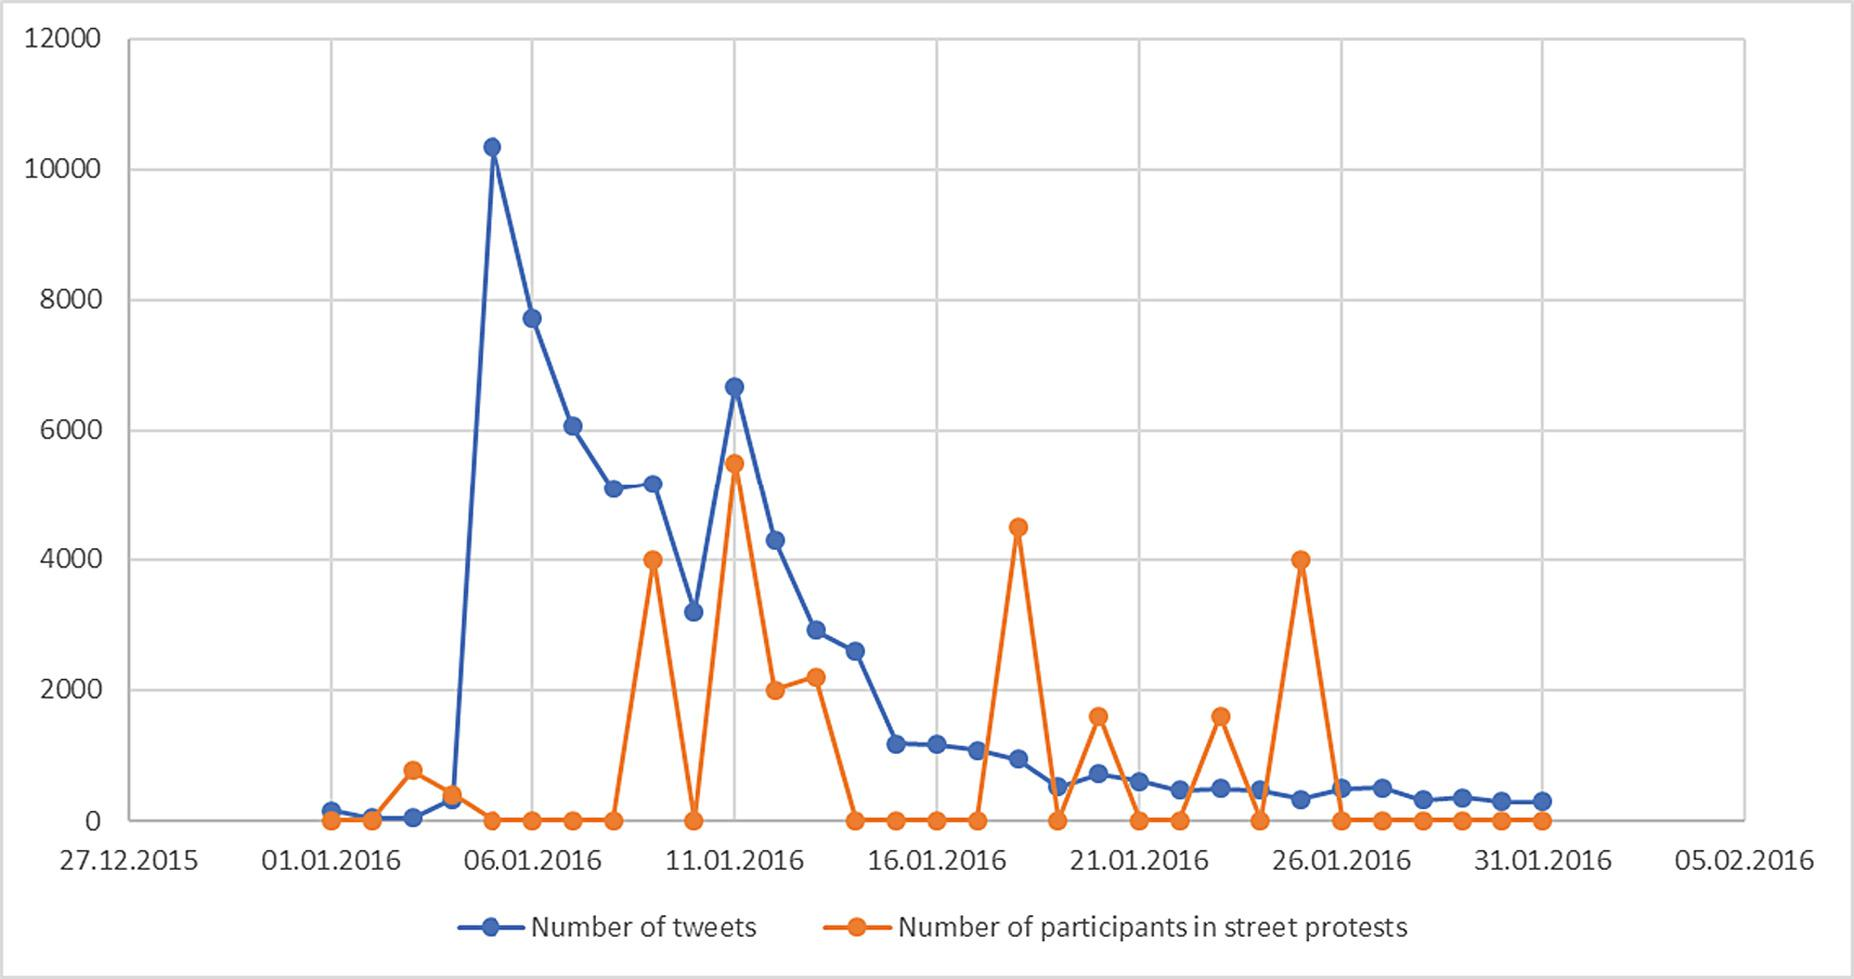
\includegraphics[scale=1.0]{onlineDiscussionTimeSeries}
	}
	\caption{Time series for online discussion and offline events.}\label{fig:onlineDiscussionTimeSeries}
\end{figure}

Granger causality test can statistically determine when one variable precedes and predictively explains another variable \cite{GroshekCloughGroshek} in case when the influence of one 1-dimensional time series parameters \((xt)\) on another time series parameters \((yt)\). The Granger causality analysis are carried out by evaluating of two types of regression:
\[ 
yt = \alpha0 + \alpha1yt - 1 + \ldots + \alpha p yt - p + \beta1xt - 1 + \ldots + \beta1xt - p + \epsilon t
\] and
\[ 
xt = \alpha0 + \alpha1xt - 1 + \ldots + \alpha p xt - p + \beta1yt - 1 + \ldots + \beta1yt - p + \upsilon t
\]
to prove the null hypothesis \(\beta1 = \ldots = \beta p = 0\).

The regressions were carried out in a special program for statistical calculation EViews (Quantitative Micro Software, Version 10). The time lag is set at 2, the level of significance, \(\alpha\), is set at 5\%, We compared two time series -- data with number of participants and data about number of tweets. The null hypothesis about the absence of influence of online activities on the offline activities has been confirmed (Probability = 0,4696), as well as null hypothesis about absence of the opposite causal relation (Probability = 0,8315).

Hence, the idea of causal relationship between street demonstrations and Twitter communication about the event is rejected. Political activities in German cities triggered by New Year’s Eve’s sexual assaults in January 2016 and discussion about them on Twitter demonstrated an asynchronous character and do not depend on each other in the time dynamic.

\subsubsection{4. Detecting Pivotal Points via Topic Modeling}

\paragraph{4.1 The Method}
On the second step of our work with the case, we have tried an alternative methodology to detect patterns of interaction between online and offline activities. Our idea was to trace the change of topicality during the immediate aftermath of the conflict and to see whether the patterns repeat across several cases. In this paper, we look at just one case but we already see a particular pattern in interaction of topicality and protest activity.

To define the pattern, topic modeling was performed on the tweets to model the topic distribution for each day from the period of the study. The algorithm Biterm Topic Model has been chosen due to time restrictions and computational capabilities. BTM has been developed for short texts: this is an efficient algorithm that allows getting coherence topics for short text collections \cite{YanyanJiafengXueqi}.

The BTM algorithm assigns the topics to each document; then, the grouping of the messages and the corresponding topic distribution is performed, whereas the time of publication is used as a criterion for the grouping procedure. After several pre-tests with the number of topics from 20 to 200, 50 topics were chosen to perform the modeling procedure. The list of the topics with distribution coefficients \(p(z)\) for each day of the period has been visualized in a form of a heat map (see Fig.~\cref{fig:topicDistributionJan2016}).

\begin{figure}[ht]
	\centerfloat{
		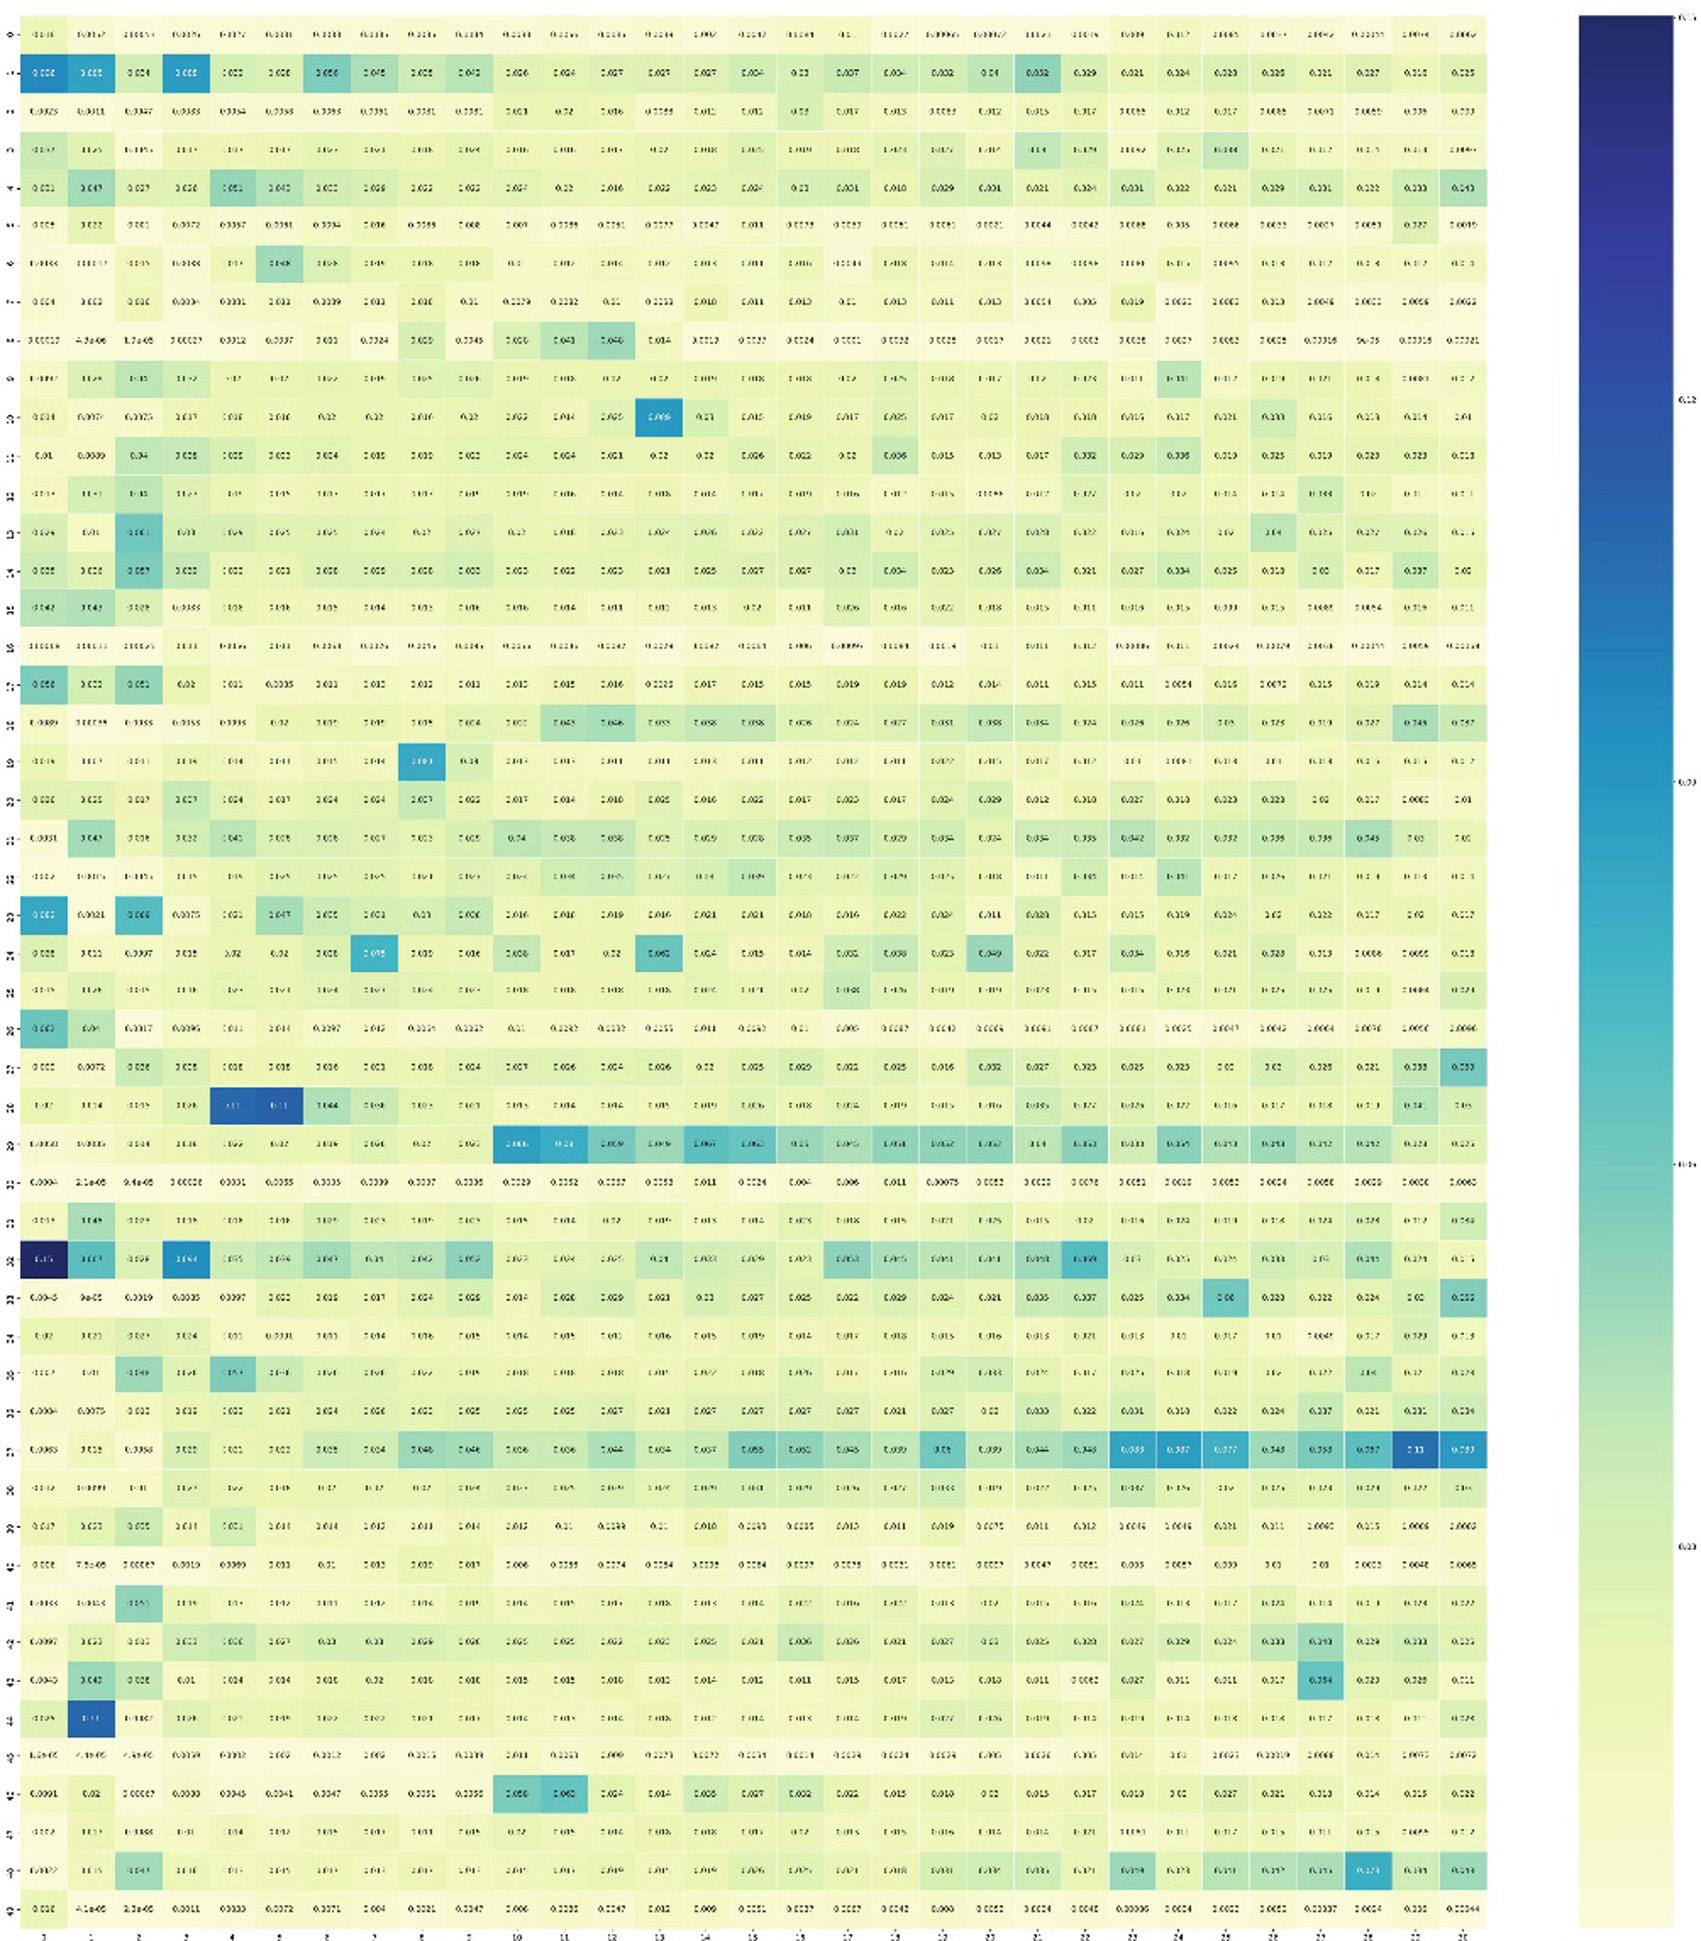
\includegraphics[scale=1.0]{topicDistributionJan2016}
	}
	\caption{Distribution of topics during January 2016 (axis \(x\)) according to their coefficients \(p(z)\) (axis \(y\)).}\label{fig:topicDistributionJan2016}
\end{figure}

To analyze the semantic structure of the discussion, we formed the list of the most salient topics. If the weight of a topic (p) on a particular date exceeded 0,047 (more than 50\% in the daily topic distribution), it indicated that the actuality of this topic has increased sharply. 26 topics that were at particular points more salient than 0,047 are unevenly distributed in the course of January 2016, with most salient topics visible in the first three days of the conflict (five topics on January 1 and 2, six at January 3). In the discussion below, the topics are listed 1 to 50 (instead of 0 to 49 on the heat map).

\subsubsection{5. Results}

As visualized on Fig.~\cref{fig:mostSalientTopicsNYE}, four topics were salient on more than five days during the period of study. Their semantic structure is listed in the Table~\cref{tab:salientTopicsSemanticStructure}. Every topic includes nominations of place, actors, and hashtags employed by the users to frame the issue.

\begin{figure}[ht]
	\centerfloat{
		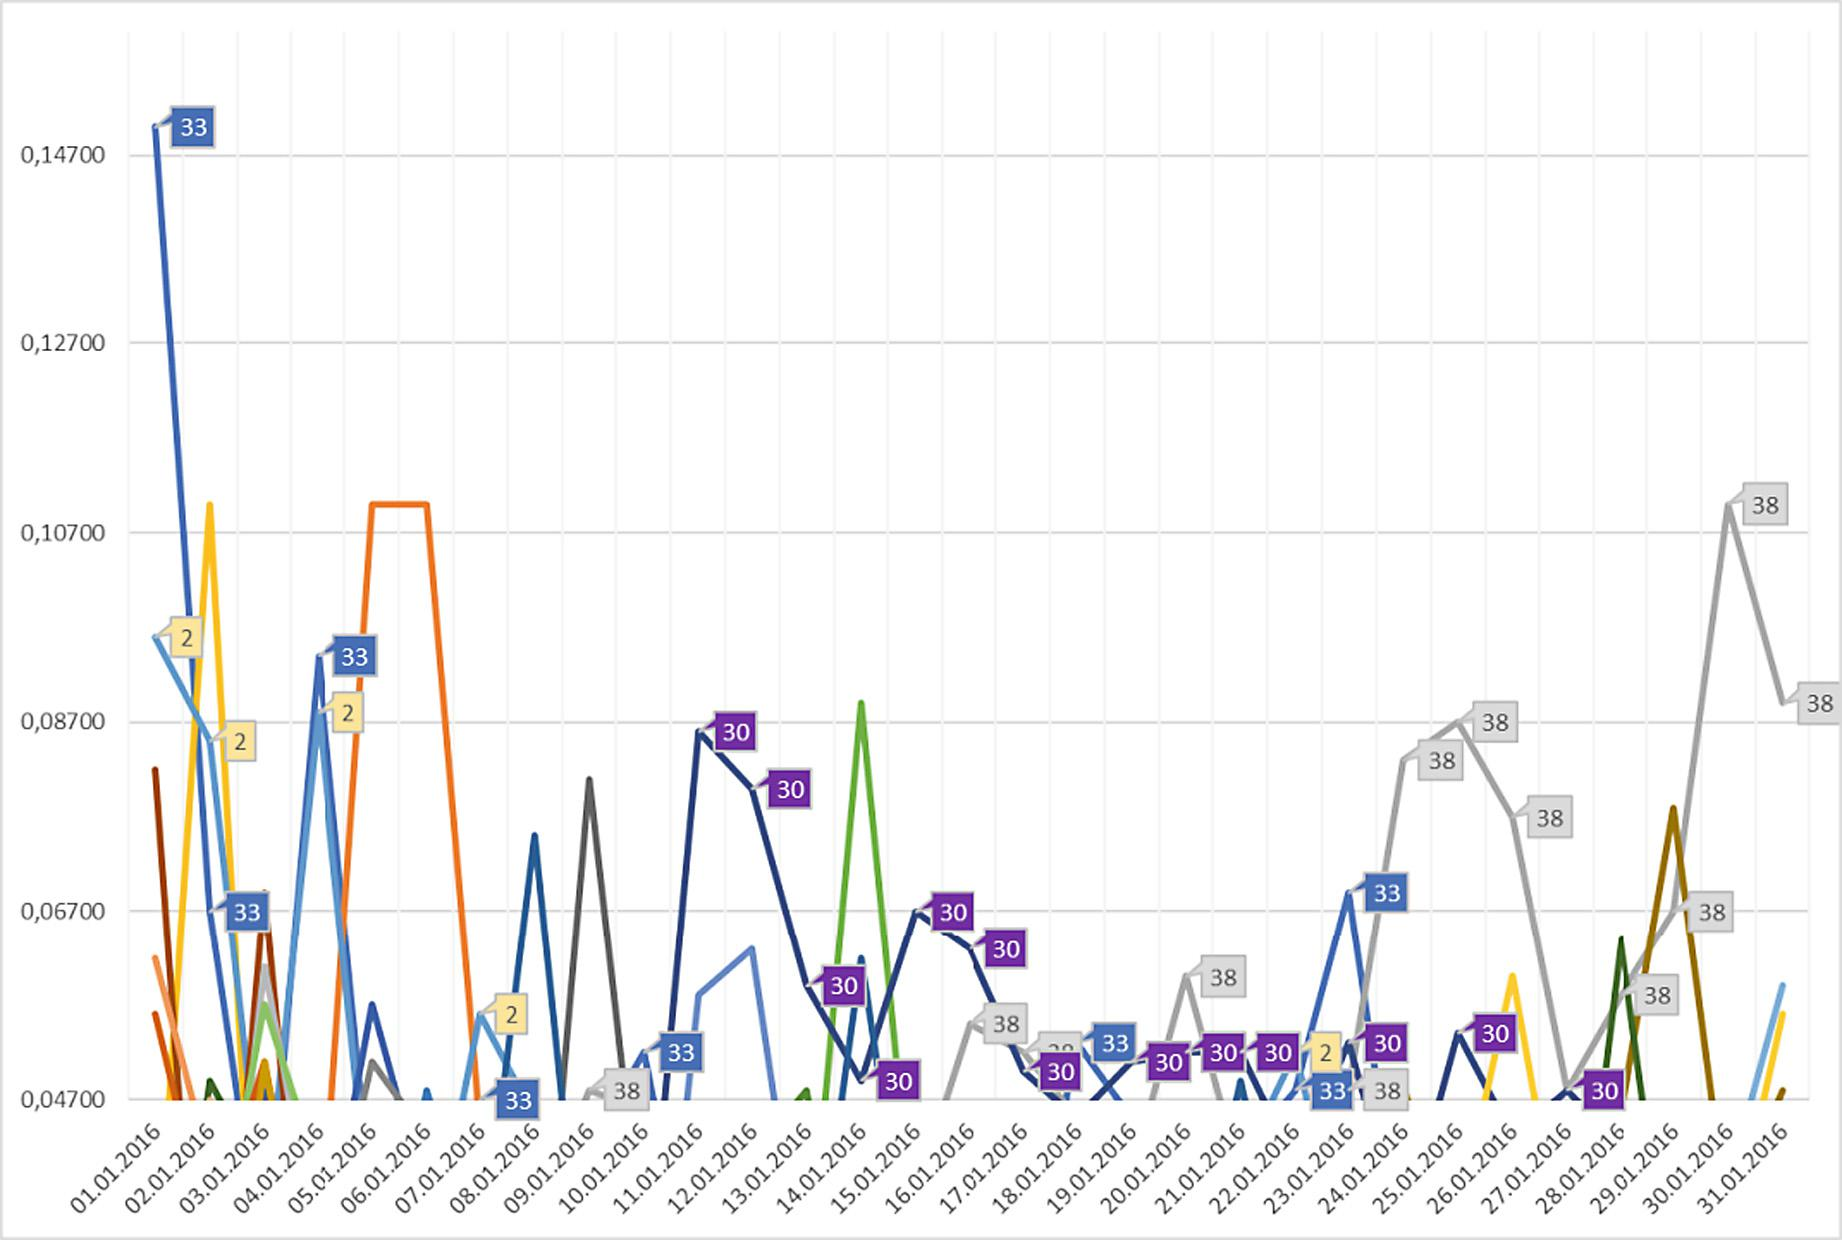
\includegraphics[scale=1.0]{mostSalientTopicsNYE}
	}
	\caption{The most salient topics in the Twitter discussion about New Year’s Eve’s sexual assaults (axis \(y =\) weight of a topic).}\label{fig:mostSalientTopicsNYE}
\end{figure}

\begin{table} [htbp]%
	\centering
	\caption{Semantic structure of the regularly salient topics.}%
	\label{tab:salientTopicsSemanticStructure}% label всегда желательно идти после caption
	\renewcommand{\arraystretch}{1.5}%% Увеличение расстояния между рядами, для улучшения восприятия.
	\begin{SingleSpace}
		\begin{tabulary}{\textwidth}{@{}>{\zz}L >{\zz}C >{\zz}C@{}} %Вертикальные полосы не используются принципиально, как и лишние горизонтальные (допускается по ГОСТ 2.105 пункт 4.4.5) % @{} позволяет прижиматься к краям
			\toprule     %%% верхняя линейка
			Topic N & Top words & Dates of saliency \\
			\midrule %%% тонкий разделитель. Отделяет названия столбцов. Обязателен по ГОСТ 2.105 пункт 4.4.5
			2 &  Ausnahmslos, gewalt, koelnhbf, rassismus, sexualisierte, frauen, sexismus, immer, sexuelle, aufschrei & January 1, 2, 4, 7, 22 \\
			33 &Koelnhbf, ausnahmslos, koeln, muslime, rapefugees, versuch, neue & January 1, 2, 4, 7, 18, 22, 23\\
			30 & Koelnhbf, koeln, polizei, medien, silvesternacht, amp, mueller & January 11 to 17 \\
			38 & Koelnhbf, ausnahmslos, merkel, amp, pegida, schon, mal, abmerkeln, brief & January 19, 20, 21, 23, 25, 27 \\
			\bottomrule %%% нижняя линейка
		\end{tabulary}%
	\end{SingleSpace}
\end{table}

Juxtaposition of the most salient topics clearly shows that there are four periods on the time-series graph when different topics dominated with a varying degree of sal- iency: January 1 to 7; January 8 to 15; January 16 to 23; January 24 to 31 (see Fig.~\cref{fig:topicDistributionPeriods}).

\begin{figure}[ht]
	\centerfloat{
		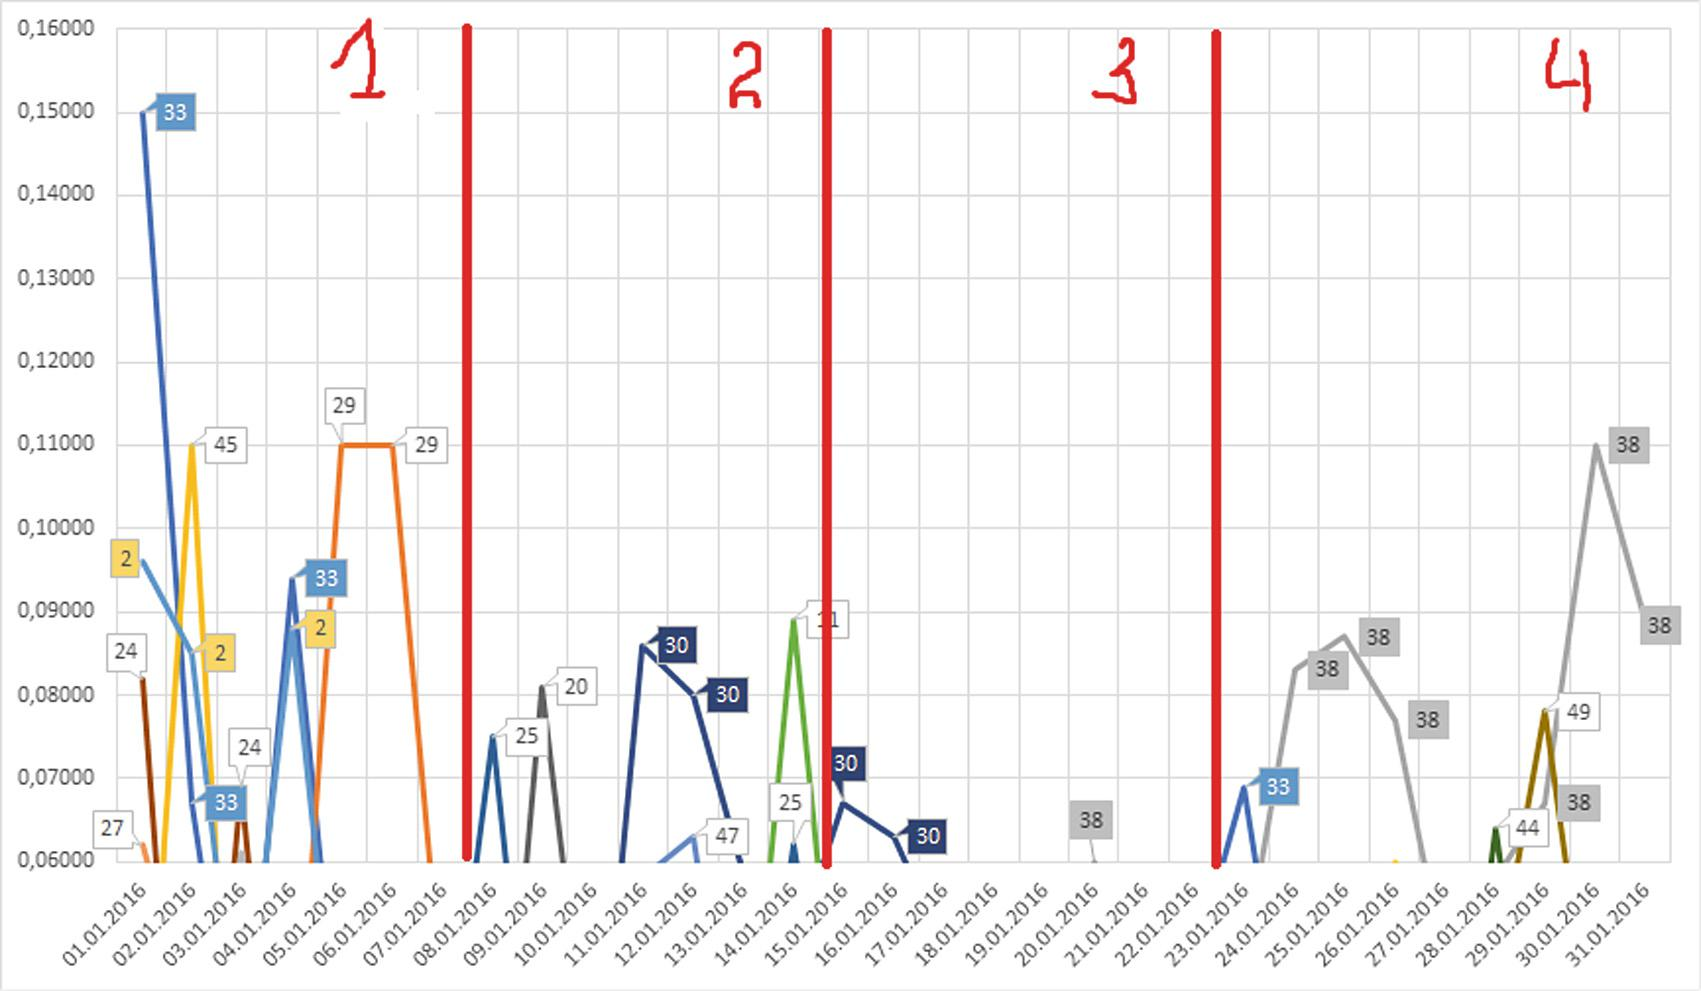
\includegraphics[scale=1.0]{topicDistributionPeriods}
	}
	\caption{Periods in topic distribution.}\label{fig:topicDistributionPeriods}
\end{figure}

In the first period (January 1 to 7, 2016), nominations among the top words define direct participants (topics N2 and N33): women (‘frauen’) against Muslims and ‘rapefugees’. Hashtags \#ausnahmslos and \#aufshrei indicate a feminist voice in the Twitter discussion: the hashtag \#aufschrei was introduced first in 2013 by feminism activist Anne Wizorek. This period was the most ‘buzzy’, according to the number of salient topics.

In the second period (January 8 to 15, 2016), topic N30 is the most salient. It demonstrates the public debate on the role of police and German media during the conflict: both actors were heavily criticized on Twitter. The second most salient topic during one day was the topic N20 that discusses more extensively political authorities who participated in the debate: Minister President of North Rhine-Westphalia Hannelore Kraft, North Rhine-Westphalia’s Interior Minister Ralf Jäger, and North Rhine-Westphalia’s parliamentarian from FDP Christian Lindner.

The third period (January 16 to 21, 2016), as the heat map shows, is a ‘gap’ period between topic N30 that is becoming less salient from its maximum on January 11, and topic N38 that increases in salience tremendously since 24\(^{th}\) of January. According to our time series analysis (see Table~\cref{tab:actionsAndStatementsGermany}), both PEGIDA and NOPEGIDA demonstrations have taken place but the number of tweets reduced significantly from more than 2500 on January 14 to less than 500 on January 23.

Topic N38 dominates the discussion in the last period (January 22 to 31, 2016). It reflects the activity of the PEGIDA movement and its supporters who use the hashtags \#abmerkeln and \#merkelmussweg -- both urge Angel Merkel to leave her Chancellor post.

We tried to trace manually whether the topics relate to the events. Concerning street actions, PEGIDA movement was mentioned only in 3 topics of 50 in our model (N21, N28, N38). Topic N21 goes beyond the saliency threshold only once, on January 2, while the first street action of PEGIDA supporters happened on January 4. Topic N28 passes the salience threshold only once, on January 31, after a wave of street actions. Topic N38 has been most salient before the street protests on January 18 as well as on the days when street actions took place (January 9, 20, 23, and 25). It reaches the highest level of salience (weight of a topic (p) exceeds 0,08) on January 24 and 25 in comparison to \(p = 0,048\) on January 23. In both cases, on January 18 and 25, the biggest number of participants took part in PEGIDA street actions (4000, as estimated by German media reports).

On January 14, Minister President of North Rhine-Westphalia Hannelore Kraft presented the package of actions to be taken for improving security and integration. Salient topics do not mention Kraft and do not relate directly neither to N11 (most salient, \(p = 0,089\), mentions the Head of Cologne’s police Albers fired on January 4 and North Rhine-Westphalia’s Interior Minister Ralf Jäger) nor to N25 (mentions political parties CDU/CSU, AFD, SPD and FDP), nor to N30 (mentions feminist hashtags \#aufschrei and \#ausnahmlos as well as popular hashtag related to the mayor Reker \#einearmlaenge). On the next day, the only topic N30 exceeded the level of \(p > 0,047\). In this case, we do not observe any connection between a political act of authorities and Twitter debate.

\subsubsection{6. Conclusions}

Scholars have tested a wide range of factors influencing political mobilization and, in particular, mass participation in a street action. Internet penetration, online user behavior and participation in online discussions were studied among other parameters. We argue that online behavior cannot be seen is a sole, dominant predictor for spillovers of protest to the street, as scholars that focused on interrelation between online and offline political activities have revealed controversial evidences on the causal relations between them.

In this paper, we presented the pilot study of relations between online and offline political activities triggered by New Year’s Eve’s sexual assaults in Germany 2016. The Granger causality test conducted in a way suggested by authors \cite{BastosMerceaCharperntier}, has failed, partly because the case study is characterized with the lack of parameters and data to compare the level of commitment among Internet users and street actions participants. In such cases, alternative ways to assess the relations between online and offline activities might be needed.

To prove the inter-relation between online discussion and offline political activities, new criteria and parameters are needed to be operationalized. To reveal these parameters for further research, we analyzed the data with the help of topic modelling that has visualized how the topics develop through the online debate.

Based on the results of the topic modeling, we juxtaposed the development of the most salient topics and the timing of the offline political activities in January 2016. Four periods were revealed, including the ‘gap’ period where topic saliency was the lowest. While in two first periods authorities and their (dis)activities were the main focus of the discussion, the fourth period is dominated by the topic that reflects far-right discourse (N38).

Several topics have gone beyond the saliency threshold (weight of a topic \((p)\) exceeding 0,047) before, on, and after the days of street actions; the most visible topics have also reached the highest level of saliency (weight of a topic \((p)\) exceeding 0,08) before the offline events. These intersections should be studied in a more nuanced way, \textit{i.a.} hour by hour. Hence, topic modeling has provided evidence that visibility of political activists precedes the street actions they organize. Moreover, the rapid change of the level of saliency that we observed for the topic N38 took place before the day the biggest number of participants took part in PEGIDA street actions in two cities simultaneously on January 25. If the peak of the topic in an online discussion precedes the mass participation in an offline street action, one might argue that the platform participated actively in forming of protest consensus. Rapid appearance of a peak within a topic, just like we observed for topic N38, might be a predictor for the forthcoming successful mobilization.

We assume that the Granger causality test might provide more accurate results in cases like New Year’s Eve’s sexual assaults in Germany 2016 if the level of street activity is examined against the level of salience of the dominant topics. Significant changes in the level of salience (rapid appearance of a peak with the topic distribution, as observed for topic N38) might be a predictor for the forthcoming successful mobilization. For more conclusions, we will in future compare several case studies of the same nature, to see whether the patterns that we have discovered for Cologne repeats for other countries and cases within Germany.

\section{Методы анализа тональности контента}\label{sec:ch5/sect3}

\subsection{Sentiment analysis for ad hoc discussions using multilingual knowledge-based approach}\label{subsec:ch5/sec3/sub1}

\subsubsection{1. Introduction}

Recently, the number of active users of social networks has increased many times, for example according to the website statista.com: Twitter has 313 million active users per month, 100 million users per day and 500 million tweets are published daily; Facebook has 1.79 billion active users per month, 1.18 billion per day. Such activity also influences people’s reaction to various social, political and economic events in the world. As a result, this means that such events are covered and distributed in social networks several times faster than in other media. Various discussions that arise as a result of any major events have an unpredictable structure of development and a number of specific properties, such as the peculiarity of user interaction among themselves, their relationship to the event, etc. Such discussions are called ad hoc discussions. For example, on Twitter and other social networks on major world events, there are long and branched discussions, the collection and analysis of which is a non-trivial task.

A separate task in the analysis of social networks is to determine the sentiment of the posts of users that were published in the context of any discussion, in particular, in the ad hoc discussion. Sentiment analysis \cite{Liu} is a class of methods that combines algorithms of computer linguistics, semantic and lexical analysis, as well as machine learning. One of the serious problems of analyzing the tonality of texts is the separation of a useful part of the text, that is, one that contains really useful information, and noise -- information that either does not affect the positivity or negativity of the statement, or complicates the precise definition. Another problem that the authors are also trying to solve is the analysis of short texts. So, for example, social network Twitter seriously differs from many other platforms with its limitations on the length of the post, which in 2018 is only 280 characters. This suggests that the messages in in most cases can contain only some essential information, or be spam and noise, detection and screening of which is another task. In addition, another distinctive feature of Twitter is the opportunity to conduct large and branched discussions on certain topics: whether it’s politics, economics, sports, etc., which can be easily monitored using hashtags.

In this paper, taking into account the specifics of short messages on Twitter, the authors set the task to develop a knowledge-based method for sentiment analysis of user messages in two major ad hoc discussions (Ferguson unrest (USA) and Biryuliovo bashings (Russia)). One of the problems that we are trying to solve is the lack of a decent russian lexicon. In fact, there is not one complete and accessible. There have been attempts to create such lexicons, but their effectiveness has not been verified to date. So we create a dictionary of russian affective words and compare its effectiveness with english lexicons.

\subsubsection{2. Current Research in Sentiment Analysis}

Researchers have studied almost all the main aspects of the problem. In their paper \cite{SchullerKnaup}, B. Schuller and T. Knaup propose an approach based on N-Grams and support vector machines \cite{ScholkopfCristianini}, which is very popular among researchers nowadays. In addition, the authors propose an approach that does not require pre-tagged data, and operates on the basis of knowledge-based resources, as well as linguistic analysis. They describe the use of online dictionaries containing both information about words and phrases, and the connections between them. Also, the article considers the possibility of using information about parts of speech of words to improve the accuracy of the analysis results. Also, K. Yessenov \cite{MisailovicYessenov} presented an analysis of the tone of comments to the reviews on films. The authors empirically studied the effectiveness of machine learning algorithms in the classification of text messages to their semantic value. The researchers used comments on the articles on the pop- ular Digg.com resource and investigated them for positivity and negativity. In \cite{RavindranSuchdevKotkar} the authors consider the possibility of combining knowledge-based methods and machine learning algorithms for analyzing users’ messages on the Twitter social network, which differ in their length. In the context of their study, they create a feature vector that contains such information as the number of positive and negative words, emoji and hashtags, and then classify data using machine learning algorithms (in particular, the support vector machine \cite{ScholkopfCristianini}). In addition, the issues of data preprocessing, use of metadata of each tweet and ways of its representation for further classification are considered.

Previous works also described methods for detecting influencers and ordinary users of ad hoc discussions. Often, users with fewer views and likes are more influential than others. This is shown in the articles \cite{BodrunovaLitvinenkoBlekanov2016,BodrunovaLitvinenkoBlekanov2017}, in which users and their connections were presented in the form of graphs and evaluated by various measures of centralities, such as pagerank and betweenness, as well as an expert analysis of the sentiment of users.

There are not many works devoted to the analysis of tonality in Russian. In \cite{BelyatskayaZagibalovCaroll} authors describe comparable corpora of book reviews in English and Russian and present experiments with a sentiment classification system. In \cite{ChetviorkinLoukachevitch} researchers consider a new approach for domain-specific sentiment lexicon extraction in Russian. They propose a set of statistical features and algorithm combination that can discriminate sentiment words in a specific domain. The extraction model is trained in the movie domain and then utilized to other domains.

\subsubsection{3. Proposed Sentiment Analysis Method}

The knowledge-based method developed by the authors includes the following steps:
\begin{enumerate}
	\item Construction of affective dictionaries.
	\item Data preprocessing.
	\item Classification.
\end{enumerate}

\paragraph{3.1 Construction of affective dictionaries} 
To analyze the sentiment of users’ messages in the study of major ad hoc discussions in the social network Twitter authors used a knowledge-based approach based on the construction and application of tagged dictionaries of positive and negative words. These dictionaries were constructed for English, French, Italian, Russian and Spanish languages according to the following principle. The most complete tagged list of English positive and negative words from open sources was selected. In our case, a dictionary that was constructed during the work of the University of Illinois at Chicago staff was used and is being expanded since then \cite{EnglishOpinionWords}. This dictionary contains approximately 6785 words. Initially there were 2005 positive words and 4780 negative words. Further, the procedure of extending the resulting dictionary was applied by adding synonyms from the WordNet database to it as follows. The authors developed a software component that matches each word from the already existing dictionary with a list of synonyms. As a result of the procedure, the dictionary consisted of 5787 and 11660 positive and negative words, respectively. This component checked the extended dictionary for repetitions, and, in case of occurrence of any identical words, deleted them. Using the machine translation procedure, new dictionaries were constructed in the appropriate natural languages. Since the results of the machine translation the repetitions could be formed again, the resulting dictionaries passed the procedure of removing duplicates. As a result of the performed actions, the dictionaries of Russian positive and negative words now consist of 3832 and 3890 words, respectively.

\paragraph{3.2 Preprocessing}
In order to improve the results and improve the accuracy of solving the classification problem, it is first necessary to bring the tweets to a normal view. This process is called normalization and, in addition to bringing all the symbols to the lowercase, includes following three steps.

\textit{3.2.1 Stop-words removal.} First of all, when processing the case, it is necessary to delete all noise words or stop-words. Stop-words are words that are often found in the language and carry almost no semantic meaning. For example, in English, such words can be prepositions (in, on, at, etc.), conjunction (and, but, for, etc.) and other function parts of speech. In addition, numbers, dates and times are also words that are removed from the tweet. In the context of processing tweets, we also remove all the mentions, that are, links to other Twitter users that start with the \@ symbol, as well as all possible links to third-party resources and sites that are not carrying any practically useful information and basically are noise. Since we do not have a tool capable of evaluating the significance of punctuation marks, we also expose them.

\textit{3.2.2 Tokenization.} The next step is to tokenize the text. This means we have to separate the text into significant units (tokens) for further processing. In the case of tweets, the most optimal size of token is one word. Therefore, after the separation, the tweets will be represented by a list of words that remained after the process of stop-words removal.

\textit{3.2.3 Stemming.} The third and final step is stemming \cite{SavoyDolamic}. Stemming is the process of extracting the basis of a word, which in this case may not coincide with the root of the word. In tasks of text classification, stemming is necessary first of all in order to reduce the dimensionality of the problem and increase the productivity of the classifier. There are many stemming algorithms for different languages. The most common is the stemmer of Martin Porter, developed originally only for the English language. But later the main idea of the algorithm was used to create the project "Snowball" and stemmers for different languages. Snowball is a small programming language designed for writing stemming algorithms. In the context of this study, we also subjected the dictionaries constructed in the previous paragraph to the stemming, since in the process of classifying it is necessary to define the polarity of a word, which is fully expressed in its basis.

\paragraph{3.3 Classification}
Our classification algorithm is fed to the input received after a preprocessed list of words that could affect the classification. Each word of this list is checked for the presence in dictionaries of positive and negative words constructed in the previous section. Ultimately, the number of positive and negative words in the list is counted. If the number of positive tokens exceeds zero and the number of negative tokens is zero, then the corresponding tweet is considered as positive, if the number of negative tokens exceeds zero, and the number of positive tokens is zero, then tweet is negative. In all other cases: if these numbers are equal or in some tweet there are both positive and negative tokens, then the tweet is marked as neutral. This approach shows different results on different test cases. This is our first approach.

We also offer a more obvious version of this classifier. In this version, the algorithm is also fed with a list of words obtained after preprocessing, and the number of occurrences of positive and negative words is also considered. However, those tweets whose word lists contain more positive than negative elements are considered positive, tweets that contain more negative than positive words are getting negative tag. Finally, tweet is marked as neutral if numbers of positive and negative words are equal. In this approach, you can see that in most cases tweets will be classified as positive or negative and only a small part of them will be neutral. Because of the fact that in this paper we consider the ad hoc discussion, we propose some adjustment of this algorithm: depending on the topic and features of the current discussions, it is possible to introduce a measure that would allow more precise definition of neutrality of some tweet. In other words, the number of tweets that would be labeled as neutral in the original version of the algorithm would be greater. The proposed metric \(m\) is introduced as follows:
\begin{equation}
	\label{eqn:31}
	m = \frac{p - n}{N}
\end{equation}
where \(p\) is number of positive words in tweet, \(n\) -- of negative words and \(N\) is total number of words in tweet. After the introduction of this metric, you can add to the algorithm some coefficient (let’s say \(c\)), which would be the threshold value for neutral tweets. In other words, if the number of positive and negative words differs slightly, then the tweet is considered neutral. This approach allows you to customize the work of the algorithm, depending on the characteristics of a certain ad hoc debate.

\subsubsection{4. Experiment}
An experiment was conducted to assess the quality of the developed method in three modifications. There were two qualitative measures used: accuracy score and f1 score \cite{Powers}. As a test data there were chosen two real large ad hoc discussions \cite{SmoliarovaBlekanovBodrunova} in Russian and English.

\paragraph{4.1 Test cases description and tagging}
In this paper authors have the opportunity to analyze the data of ad hoc discussions in the social network Twitter of two well-known events: Ferguson unrest (USA) in August 2014 and Biryuliovo bashings (Russia) in October 2013. For each of the events above, there was compiled a list of popular hashtags that describe it:
\begin{enumerate}
	\item Biryuliovo: \#бирюлево, \#мигранты, \#овощебаза, \#зейналов.
	\item Ferguson: \#ferguson.
\end{enumerate}
As a result of the collecting and processing the set of hashtags, we got the following data:
\begin{enumerate}
	\item Biryuliovo: Number of users who have published their tweets in the period since 1st of October 2013 till Thirty-first of October 2013 is 3574. Number of published posts is 10215.
	\item Ferguson: Number of users who have published their tweets in the period since twenty-second of August 2014 till Thirty- first of August 2014 is 70018. Number of published posts is 193812.
\end{enumerate}
On the Figures~\cref{fig:fergusonPublicationActivity} and~\cref{fig:biryulievoPublicationActivity}, one can observe the publication activity of users of discussions about Ferguson and Biryulyovo, respectively. It can be seen that the ad hoc discussions have a different structure: only one "splash" of activity is visible in the discussion of Biryulyovo and the discussion of the situation in Ferguson that has not ceased throughout the week.

\begin{figure}[ht]
	\centerfloat{
		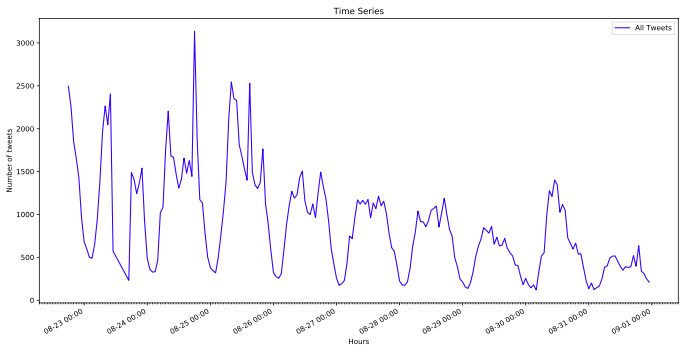
\includegraphics[scale=0.5]{fergusonPublicationActivity}
	}
	\caption{Periods in topic distribution.}\label{fig:fergusonPublicationActivity}
\end{figure}

\begin{figure}[ht]
	\centerfloat{
		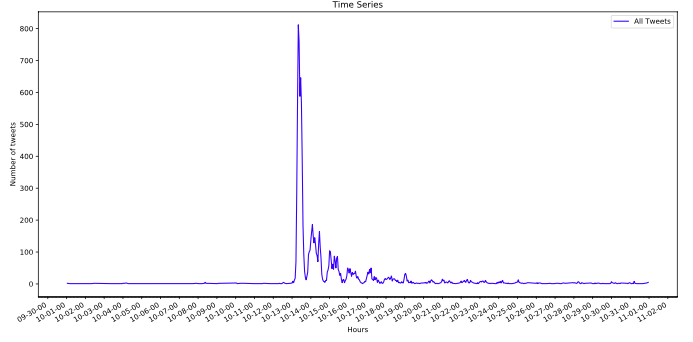
\includegraphics[scale=0.5]{biryulievoPublicationActivity}
	}
	\caption{Periods in topic distribution.}\label{fig:biryulievoPublicationActivity}
\end{figure}

To calculate the qualitaty measures, the authors performed the tagging of the above-described data sets as follows:

\begin{enumerate}
	\item For each ad hoc discussion, lists of top-100 users were compiled according to the number of published messages, as far as betweenness centrality and as far as pagerank centrality \cite{BodrunovaLitvinenkoBlekanov}.
	\item Aggregation of three top-100 lists and deletion of duplicate users. As a result, 213 users were obtained in the Biryuliovo case and 200 in the Ferguson case.
	\item By the aggregated list of users in the Biryuliovo case there were selected all user messages, the total number of which was 3885. In the Ferguson case there were collected just fifteen random messages by each user in order to keep size of the collection slightly equal to the size of Biryuliovo collection.
\end{enumerate}

\paragraph{4.2 Results}
In the course of carrying out the work described above, the problem of the analysis of the ad hoc discussions in the social network Twitter was considered. The authors presented a multi-lingual approach, which is based on the construction and use of affective dictionaries for Russian language and compare it efficiency to expanded existing English lexicon. To assess the quality of the three modifications of this approach, measures accuracy score and f1 score were used on manually annotated data. These results are presented in the Table~\cref{tab:fergusonAccuracyF1}. Results for Biryuliovo case are represented in the Table~\cref{tab:biryliovoAccuracyF1}. These tables show that our best approach gives 0.7 f1 score which is the average result in English \cite{KingHopkins,RavichandranRao}. The results for the Russian dictionaries are slightly lower than the average English. We assume that this is due to the imperfection of machine translation and the difference in the structure of Russian and English.

\begin{table} [htbp]%
	\centering
	\caption{Accuracy and F1 score for Ferguson.}%
	\label{tab:fergusonAccuracyF1}% label всегда желательно идти после caption
	\renewcommand{\arraystretch}{1.5}%% Увеличение расстояния между рядами, для улучшения восприятия.
	\begin{SingleSpace}
		\begin{tabulary}{\textwidth}{@{}>{\zz}L >{\zz}C >{\zz}C >{\zz}C@{}} %Вертикальные полосы не используются принципиально, как и лишние горизонтальные (допускается по ГОСТ 2.105 пункт 4.4.5) % @{} позволяет прижиматься к краям
			\toprule     %%% верхняя линейка
			& First version & Second version & With \(m\) metricy \\
			\midrule %%% тонкий разделитель. Отделяет названия столбцов. Обязателен по ГОСТ 2.105 пункт 4.4.5
			accuracy score  & 0.65 & 0.49 & 0.62\\
			f1 score & 0.70 & 0.52 & 0.66 \\
			\bottomrule %%% нижняя линейка
		\end{tabulary}%
	\end{SingleSpace}
\end{table}

\begin{table} [htbp]%
	\centering
	\caption{Accuracy and F1 score for Biryliovo.}%
	\label{tab:biryliovoAccuracyF1}% label всегда желательно идти после caption
	\renewcommand{\arraystretch}{1.5}%% Увеличение расстояния между рядами, для улучшения восприятия.
	\begin{SingleSpace}
		\begin{tabulary}{\textwidth}{@{}>{\zz}L >{\zz}C >{\zz}C >{\zz}C@{}} %Вертикальные полосы не используются принципиально, как и лишние горизонтальные (допускается по ГОСТ 2.105 пункт 4.4.5) % @{} позволяет прижиматься к краям
			\toprule     %%% верхняя линейка
			& First version & Second version & With \(m\) metricy \\
			\midrule %%% тонкий разделитель. Отделяет названия столбцов. Обязателен по ГОСТ 2.105 пункт 4.4.5
			accuracy score  & 0.57 & 0.41 & 0.55\\
			f1 score & 0.65 & 0.46 & 0.6\\
			\bottomrule %%% нижняя линейка
		\end{tabulary}%
	\end{SingleSpace}
\end{table}

\subsubsection{5. Conclusion}

In this article, authors proposed a multi-lingual approach to the analysis of ad hoc discussions and, in particular, the sentiment analysis of messages in such discussions. The presented algorithms showed quite good results, which were represented in the relevant tables, taking into account the specifics of the given discussions. In the future work, the authors plan to develop this approach and compare it with the work of such classification algorithms as the support vector machines.

\subsection{When emotions grow: cross-cultural differences in the role of emotions in the dynamics of conflictual discussions on social media}\label{subsec:ch5/sec3/sub2}

\subsubsection{1. Introduction}

The spread of affective content on social media, as well as user grouping based on affect \cite{Papacharissi}, has been a focus of scholarly attention due to multiple reasons. Emotional content is seen mostly as a threat to the democratic quality of public discussions \cite{Cortese}, as it undermines its integrity and rationality \cite{BadjatiyaGuptaGupta}, as well as its civility and constructive character \cite{BurnapWilliams}, especially when one deals with hate speech and toxic expressions \cite{ParkFung,GeorgakopoulosTasoulisVrahatis}.

Despite the evident necessity to learn how emotions work within the discussion, we lack evidence on what roles various particular emotions play in the dynamics of discussions on social media. Detection of particular emotions has been mostly linked to political emotionality and political functions of emotions \cite{Lyman,TicentoCloughHalley,HeaneyFlam,WahlJorgensen}, as well as their linkage to other features of content like fake news \cite{VosoughiRoyAral}.

The substantially negative role of hate speech is practically non-questioned today; but several works still draw attention to controversial relations between freedom of speech and hate speech \cite{Dorsett,Cammaerts} and to the possible use of offensive language in positive sense in discriminated communities like LGBTQ \cite{WaseemDavidsonWarmsley}. Another potentially positive role of emotional content (negative just as well as positive) might lie in spurring the discussions, providing them flame and substance and not letting them ebb.

In this paper, we explore just two aspects of this issue, namely -- the growth of emotional load in conflictual discussions and the relations between the number of overall users in the discussion and the angry and compassionate ones.

For this, we use the data from three highly conflictual and emotionally polar discussions, more or less territorially localized, despite potential global participation on Twitter. Use of three discussions from different communicative cultures will allow us generalize on the nature of the relations between the overall growth of the discussion and its highly emotional content.

To explore the discussion bulk, we collected the data via Twitter crawling, then coded the emotions with the help of native speakers, then taught the machine to recognize the emotions, and then detected the users who used emotional speech and reconstructed the hourly graphs of the discussions, as well as time series. We have also performed Granger test to spot the relations between the number of emotional and neutral users in the discussions.

The remainder of the paper is organized as follows. Section 2 discusses our idea of the emotions as discussion drivers. Section 3 poses the hypotheses, and Sect. 4 describes the data collection procedures, sampling, and the method of detecting emotions. Section 5 provides and discusses the results.

\subsubsection{2. Emotions Aggregated: What Can They Tell?}

Emotional contagion theory \cite{HatfieldBensmanThornton} adapted for social media suggests that diffusion of emotions happens on individual level, via direct one-time contact with emotionalized content \cite{CovielloSohnKramer}. Individual emotions, though, play a key role in group behavior online, as they form the so-called ad hoc discussions \cite{BrunsBurgess} of affective publics \cite{Papacharissi} and, thus, matter more on the aggregate level and might work differently from what is expected, especially in fast-growing conflictual discourse online. Other theories, like theories of social influence or social learning \cite{Young}, suggest multiple, hierarchical, and/or topically-restricted contacts of users with emotional content; whether these limitations are also true for how the emotions grow and spread collectively, still remains unclear.

The idea of affective agenda \cite{ColemanWu} implies that the dynamics of an emotional discussion might be dependent on mood changes or spillovers from group to group, language to language, or topic to topic. Also, the relations between various emotions might be a com- petitive one, since they work as the polarizing agents within the discussion: anger may overcome fear, and denial might beat compassion. A shockingly strong example of this is, of course, the case of \textit{Charlie Hebdo} which polarized the discussion participants to the extent of creating formally opposing hashtags (‘jesuischarlie’ and ‘jenesuispascharlie’, representing compassion and its rejection, anger, and discontent).

The change of affective agenda or mood within the discussion might lead to its growth (or even outburst) or ebbing, and this question remains under-explored. We suggest that emotions of different stance (positive/negative) may spur/slow down the discussions in various ways.

\subsubsection{3. The Research Hypotheses}

In this paper, we have posed three hypotheses:

\begin{itemize}
	\item H1. In all the three conflictual discussions under our scrutiny, the dynamics of emotions will go ahead of the general discussion dynamics: the number of emotional users will grow and diminish faster than the number of emotional tweets.
	\item H2. In all the three discussions, the dynamics of the number of involved users will depend on the dynamics of the number of emotional users.
	\item H3. The dynamics of compassion and anger will differ in all the three discussions and will not correlate within the cases.
\end{itemize}

We will also qualitatively describe the picture we see on the web graphs and on time series graphs, to contextualize and reflect more on the received data. By analyzing the co-dynamics of the overall discussions and these two emotions we can conclude whether the pattern of the spread of emotions and its link with the discussion dynamics is the same in various language segments of Twitter.

\subsubsection{4. Data Collection and Methods of Research}

\paragraph{4.1 The Cases Under Scrutiny}

We analyze the spread of two polar emotions -- anger and compassion -- in three Twitter discussions on inter-ethnic conflicts, namely:

\begin{itemize}
	\item The Ferguson unrest, USA, 2014: number of users who published tweets -- 70018, total number of messages -- 193812;
	\item The Charlie Hebdo shooting, France, 2015: number of users who published tweets -- 238491, total number of messages -- 505069;
	\item The mass harassment of women by the re-settlers from the Arab world in Cologne, Germany, in the New Year night of 2015-2016; number of users who published tweets -- 99981, total number of messages -- 215253.
\end{itemize}

The overall number of tweets collected based on the relevant hashtags and keywords is actually much bigger. The data we use were collected by our Twitter crawler in the aftermath of the conflicts and include altogether over 2,5 M tweets. The samples described above resulted from the fact that we selected the mono-language parts of the discussions only -- German for Cologne, French for Charlie Hebdo, and English for Ferguson. We have also cleaned spam, non-relevant tweets, and hashtag-only tweets.

\paragraph{4.2 Emotion Detection}

To be able to detect emotions, we have used an enhanced SVM-based approach with the use of Numpy and scikit-learn libraries. As we have been working with multi-lingual sentiment analysis for several years, we have modified the approach with two features. First, the experiments have shown that elimination of stop words from tweets actually diminishes the quality of the classifier. Thus, the stop words have been returned to the initial dataset, which has raised the quality by 4-5\%. Second, we have experimentally found the streaming hyper-parameters and adjusted them: the regularization parameter was 0.9, and we have also used the linear nuclear function and the OVR function. We have also spotted that, in several cases, the machine tended to over-learn; thus, we have balanced the samples to reach better results.

Tweets from real-world discussions, despite we have used the well-preprocessed datasets, remain one of the ‘noisiest’ types of textual data; this has cast some negative impact upon the quality metrics of emotion detection. This is why we have used quite large collections for hand coding. We have selected the tweets for hand coding by the procedure described in our earlier works \cite{BodrunovaLitvinenkoBlekanov2017,BodrunovaBlekanovSmoliarova}, by selecting influential users by nine parameters -- four absolute ones (the number of posts, retweets, likes, and comments) and five graph-dependent ones (in-degree, out-degree, degree, betweenness and pagerank centralities). The top users’ tweets constitute the samples for coding. Altogether, we have coded: for Germany -- 13,620 tweets, for the USA -- 7200 tweets, and for France -- 7433 tweets.

We have received the following best levels for the quality metrics (see Table~\cref{tab:threeCasesQualityMetrics}).

\begin{table}[ht]%
	\centering
	\caption{Quality metrics for emotion detection for the three cases.}%
	\label{tab:threeCasesQualityMetrics}% label всегда желательно идти после caption
	\begin{adjustbox}{width=1\textwidth}
		\small
		\begin{tabular}{ c  c  c  c  c  c  c  }% Вертикальные полосы не используются принципиально, как и лишние горизонтальные (допускается по ГОСТ 2.105 пункт 4.4.5) % @{} позволяет прижиматься к краям
			\toprule
			& \multicolumn{2}{c}{\makecell{Germany}} & \multicolumn{2}{c}{\makecell{The USA}} & \multicolumn{2}{c}{\makecell{France}} \\
			& Accuracy & F-measure & Accuracy & F-measure & Accuracy & F-measure \\
			\hline
			Anger & 0.7 & 0.7 & 0.77 & 0.77 & 0.78 & 0.77 \\
			Compassion & 0.75 & 0.74 & 0.8 & 0.8 & 0.84 & 0.84 \\
			\bottomrule
		\end{tabular}%
	\end{adjustbox}
\end{table}

\paragraph{4.3 Data Analysis and Visualization}

We have marked the tweet datasets by emotion; then we have aggregated the tweets per user and have calculated hourly numbers of neutral, angry, and compassionate users, according on whether they have expressed these emotions within a given hour. Thus, we have received he hourly numbers of users who were emotional, either compassionate or angry. Of course, in a small number of cases, a user could express both compassion and anger within one hour; but this mattered only within the first couple of hours, while in the course of the discussion the number of such users became negligibly small.

To visualize the results of the emotion detection, we have constructed the hourly web graphs for three days using the YifanHu algorithm from the Gephi library, as well as the time series graphs with the hourly lag. For Cologne and \textit{Charie Hebdo}, we have taken the first three days of after the trigger events; for Ferguson, we did not have such data and, thus, the three days were taken from the middle of the discussion.

To assess the inter-emotional relations (in terms of the number of users), we have used the Spearmans’ Rho.

To test the hypotheses, we have performed the Granger test with the hourly data and have also qualitatively assessed the graphs \cite{Wessa}. The results are presented below.

\subsubsection{5. Results and Discussion}

\textit{H1-H2.} When assessing the cases, we have seen that the basic pattern of the discussions is different from the expected: in general, the lines indicating the number of neutral users are generally followed by those of anger and compassion (see Fig.~\cref{fig:timeSeriesGraphs}). But, if we look at details and the results of the Granger test, the three start to diverge.

\begin{figure}[ht]
	\centerfloat{
		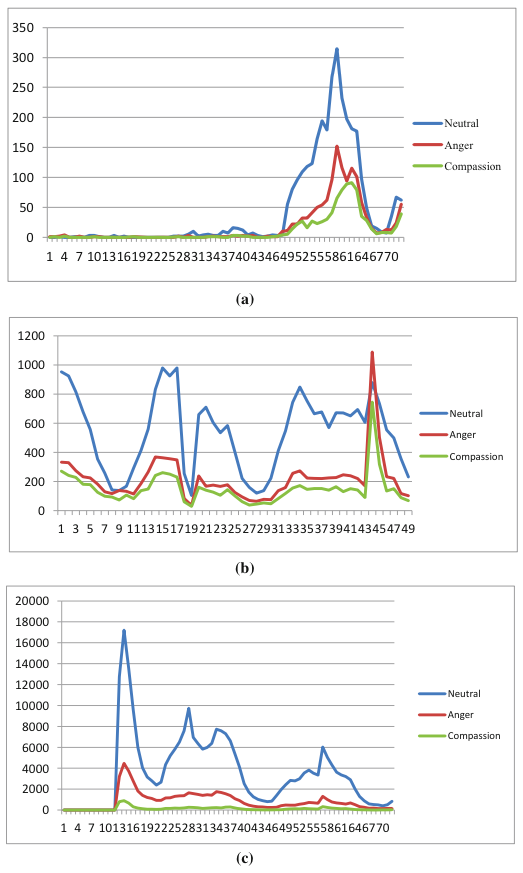
\includegraphics[scale=0.5]{timeSeriesGraphs}
	}
	\caption{a.Time series graphs, the Cologne case. b. Time series graphs, the Ferguson case. c. Time series graphs, the Charlie Hebdo case. (Color figure online)}\label{fig:timeSeriesGraphs}
\end{figure}

First of all, the three cases differ in whether the growth of the number of angry or compassionate users affects the rest of the speech in the case (see Table~\cref{tab:grangerTestResults}). In some sense, Cologne and Ferguson ‘mirror’ each other in terms of when exactly the emotional users spur the number of the neutral users. We can see from the Table~\cref{tab:grangerTestResults} that it is compassion, not anger, that plays a bigger role in predicting the number of neutral users -- that is, the very growth or ebbing of the discussions. As we see from the time series graphs, the regression shows the dependency when the discussion starts to grow. This happens with the first two days of Cologne where the journalists were reluctant to cover the mass harassment story as they were not sure how to report on the nationality of the harassers. It also happens during an outburst of emotions in the Ferguson case, on Day 3. Thus, the role of emotional content in the early-stage discussions needs to be well researched upon.

\begin{table}[ht]%
	\centering
	\caption{Quality metrics for emotion detection for the three cases.}%
	\label{tab:grangerTestResults}% label всегда желательно идти после caption
	\begin{adjustbox}{width=1\textwidth}
		\small
		\begin{tabular}{ c  c  c  c }% Вертикальные полосы не используются принципиально, как и лишние горизонтальные (допускается по ГОСТ 2.105 пункт 4.4.5) % @{} позволяет прижиматься к краям
			\toprule
			& Days 1-3 & Days 2-3 & Day 3 \\
			\hline
			Cologne anger & No No & No No & \colorbox{yellow}{11,17** 13,3**}\\
			Cologne compassion & \colorbox{green}{13,1*** No} & \colorbox{green}{8,71** No} & \colorbox{yellow}{5* 9,8**} \\
			Ferguson anger & \colorbox{violet}{No 4,13*} &	No No  & 4,76* No\\
			Ferguson compassion & \colorbox{yellow}{5,53* 8,1**} & \colorbox{yellow}{4,68* 6,52*} & \colorbox{green}{5,89* No} \\
			Charlie Hebdo anger & No No & No No & No No \\
			Chare Hebdo compassion & No No & \colorbox{violet}{No 10,2**} & \colorbox{violet}{No 5,65*} \\
			\bottomrule
			\multicolumn{4}{@{}p{\textwidth}}{%
				\hspace*{2.5em}% абзацный отступ - требование ГОСТ 2.105
				Note. Green: the test shows the dependency of the overall discussion upon these users and authors. Yellow: the test shows that the numbers of the neutral users and emotional users correlate due to a third factor.Violet: The linkage between emotional and neutral users shows the dependency of the other direction: the higher the number of neutral tweets, the higher the number of the angry and/or compassionate tweets. That is, when the discussion is boiling itself, the number of angry users also grows without any coordinated effort.
			}\\
		\end{tabular}%
	\end{adjustbox}
\end{table}

In the American case, there is also a smaller trend covered by a more general one. There are several moments in the course of the discussion when anger starts to diminish earlier than the number of the neutral tweets, and the blue line follows.

Another important conclusion is that the emotions do not grow/diminish within the discussions but have intense hourly dynamics. The ‘jumps’ of the number and connectivity of users who express anger and compassion (see Fig.~\cref{fig:fastDynamcs}, the example of Cologne) need to be further explored within the aforementioned theories of emotional contagion and/or social learning.

\begin{figure}[ht]
	\centerfloat{
		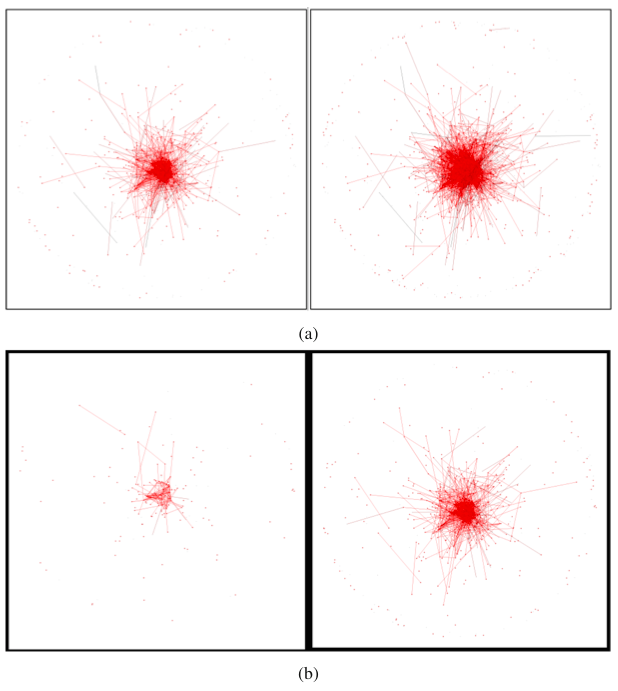
\includegraphics[scale=0.5]{fastDynamcs}
	}
	\caption{a. Fast dynamics of growth of the number of angry users within 3h (a ‘jump’ of anger), Cologne, January 4, 2016. b. Fast dynamics of growth of the number of compassionate users within 3h (a ‘jump’ of compassion), Cologne, January 4, 2016.}\label{fig:fastDynamcs}
\end{figure} 

Thus, H1 and H2, in how they were formulated, needs to be rejected: the number of the neutral users does not grow depending of the spread of emotions between emotional users. But what is also important is that the dynamics of the emotions is intensive even within the hourly perspective and that the moments when the discussion grows might depend on compassion, rather than anger. The emotions matter in the very beginning of the discussions or in the moments of discussion outbursts.

\textit{H3.} Ourthirdhypothesiswascreatedtoberejected,but,again,thisisnotwhathappens in the datasets. Thus, the correlations between the two hourly spreads of people are: for Cologne -- 0.950****, for Ferguson -- 0,988***, for Charlie Hebdo -- 0,937**. This adds to the evidence that emotional users do not lead the way and do not cause excessive discussion around them but appear within the discussion the same way as neutral users. But, when on an emotional peak, such users might create discussion outbursts.

We have tested the dependence of the discussion dynamics on the number of emotional (angry and compassionate) users of Twitter. Within the three cases, there were no similar patterns of such dependence, which might be explained by socio-cultural differences or the structure of the sample. We have also detected a special role of emotional tweets in the beginnings of the discussions and the discussion outbursts; we suggest that, in future, not users but the tweets themselves need to become the unit of analysis.

\subsection{Negative A/Effect: Sentiment of French- Speaking Users and Its Impact Upon Affective Hashtags on \textit{Charlie Hebdo}}\label{subsec:ch5/sec3/sub3}

\subsubsection{1 Introduction}

Studies of user sentiment in discussions at social networking sites, including Twitter, have formed a huge and constantly expanding research area. But there are still several important gaps in our knowledge on how social conflicts are discussed online.

First, sentiment in Twitter discussions is often analyzed without taking into account the ad hoc nature of the online conversation \cite{BrunsBurgess2015}. But, as we know, hashtagged discussions, especially conflictual ones with high potential for user polarization, tend to be more horizontal in terms of structure \cite{BodrunovaBlekanovMaksimov}, less predictable in discussion dynamics \cite{BrunsBurgees2012,BodrunovaLitvinenkoBlekanov2017}, and highly emotional due to their origin in affect \cite{Papacharissi}. This implies higher impact of personal traits of authors and of discursive features of user texts, including sentiment, upon the discussion structure. Thus, studying discussions on openly conflictual issues on social media may help detect how sentiment relates to user grouping, as well as predict the actors of potentially conflict-bearing views. Also, there is evidence that, with time, user polarization influences topic perception and news consumption \cite{DelVicarioZolloCaldarelli}, and that offline clusterization of sentiment towards a socially polarizing issues may have grave consequences for situational dynamics \cite{SalatheKhandelwal}, while positive tone in relations between local governments and citizens increases online political participation \cite{ZavattaroFrenchMohanty}. Also, the newest works show (see, e.g. \cite{KumarHamiltonLeskovec}) that in-platform conversational conflicts eventually reduce user discussion activity. Thus, it is important to assess whether sentiment is a ground for user polarization for conflictual topics.

But, second, in user sentiment studies, we observe striking scarcity of works that would link user sentiment to the discussion structural metrics and user positions in the discussion. Only rare works directly assess network metrics in relation to user sentiment (for the examples, see \cite{StieglitzDangXuan} and \cite{BigonhaCardosoMoro}). This happens despite the abundancy of works that associate sentiment with echo chamber formation in Twitter and Facebook discussions (see below). And, third, the works that would assess sentiment-based discussion structure in some comparative perspective are virtually non-existent.

Fourth, we very rarely see the cases when positive/neutral and negative hashtags could be juxtaposed. In particular, there is lack of knowledge on whether the discussion clusters tagged by emotionally opposite hashtags differ in sentiment distribution, both in terms of difference between hashtags and sentiment expressed by different types of users, e.g. ‘ordinary people’ and institutions. This happens partly because emotionalized discussions are difficult for sentiment analysis due to abundance of rhetoric expressions with indirect meanings (sarcasm, rhetoric questions etc.).

Fifth, sentiment analysis is mostly done for English-language texts, and other languages remain peripheral in sentiment detection on the global level \cite{ChenSkiena}.

We address these gaps by looking at one of the acutest online discussions of the recent years -- namely, the discussion on the \textit{Charlie Hebdo} massacre in Paris in 2015. As widely known, the hashtags \#jesuischarlie and \#jenesuispascharlie have set an example for further online discussions on violent ethnicity- and belief-based conflicts, and it was the first time when the societal value clash was so openly manifested. The research on this case and how it was discussed online is today quite extensive (for a review, see \cite{BodrunovaSmoliarovaBlekanov}), but it still lacks understanding of whether user sentiment formed distinct clusters and who were the bearers of this sentiment.

To fill these gaps, we use the approach that unites the discussion network analytics and sentiment analysis for the French language, and for the latter -- a mixture of lexicon construction and machine learning based on data from human coders.

The remainder of the paper is organized as follows. In Sect. 2, we reconstruct the scholarly discourse that links user sentiment to the discussion structure to better identify the research gaps. We also describe the current state of research on sentiment analysis for French and research upon the \textit{Charlie Hebdo} case. In Sect. 3, we pose the research questions and hypotheses. In Sect. 4, we explain our methodology, including data collection, formation of the sentiment lexicon, the discovered issues with it, and use of human coding for the machine-learning improvement of the sentiment detection. In Sect. 5, we show the results and (dis)prove the hypotheses. In Sect. 6, we discuss our results against earlier findings and explain them.

\subsubsection{2 Polar Twitter Hashtags and Their Sentiment Shape}

\paragraph{2.1 Sentiment-Based Discussion Structure: User Metrics and Echo Chambers} In the recent years, various instruments of sentiment analysis have been widely used to detect user views in relation to user groupings. Such studies mostly fall within online polarization field of studies and try to detect the so-called echo chambers based on, among other factors, user sentiment. But most of the works claim that echo chambers exist (or do not exist) based on user sentiment divergence, without assessing the relative distance of the paths between users and the users’ roles in the discussions. E.g. authors of an early work on blogs \cite{GilbertBergstromKarahalios} see individual blogs as echo chambers and, thus, by stating echo chambering based on comments, just show that individual blogs diverge in political standing. Another, more recent work \cite{HundtSchneiderElAssady} has taken a user’s ego-network of tweets/comments as an analogue of an echo chamber and used sentiment analysis to show whether these micro-structures experience divergence of views.

Works that take large homophily-based user groups as echo chambers, e.g. the one on a long-standing issue of climate change \cite{WilliamsMcMurrayKurz}, have shown that, first, sentiment does separate users in issue-based discussions and, second, is different in interactions between positively- and negatively-minded tweeters, which evidently adds to echo chamber formation. At the same time, there are works that show that ‘opinion crossroads’ also exist on Twitter, be it based on sentiment \cite{GruzdRoy} or on other features of user alignment like a user’s position towards an issue assigned manually by researchers \cite{YardiBoyd}, friendship ties \cite{ConoverRatkiewiczFrancisco}, or news sharing \cite{HerdaugdelenZuoGardMurray}. There are also works that link user metrics and/or discussion web graph structure to user sentiment. Thus, one work calls this approach hybrid \cite{AlamsyahAdityawarman} but does not go beyond just detecting the sentiment-based graph structure and showing that the seven detected communities are all heterogeneous in their sentiment. Two other works \cite{StieglitzDangXuan} and \cite{BigonhaCardosoMoro} show that sentiment analysis helps identify influencers, but do not describe who the influencers are and whether their status in the discussion is somehow linked to their offline social status.

The works that would try to juxtapose pre-defined pro/contra views on a given problem and detect sentiment within the expectedly clustered communities remain rare in sentiment analysis field. An attempt to discuss ‘positive’ (‘science’) and ‘negative’ (‘conspiracy’) statements in the discussion on misinformation was undertaken by the authors \cite{QuattrociocchiScalaSunstein,ZolloNovakDelVicario}. They have supported the long-existent claim that users come out of the online discussions with their views even more polarized and radical than before; moreover, ‘[t]he more active a polarized user [was], the more the user tend[ed] towards negative values both on science and conspiracy posts’ \cite[p.~12]{QuattrociocchiScalaSunstein}. Another work by the same group of authors \cite{DelVicarioVivaldoZollo} shows that, on Facebook, highly involved users inside echo chambers tend to express negative sentiment. Thus, we may expect that highly involved influencers may have more negative views than non-influential users in both cases. But, in contrast to this, our earlier works show that influencers in the discussions on Charlie Hebdo tend to have mixed sentiment \cite{BodrunovaBlekanovKukarkinCH}.

Out of this research, we see that: (1) event-based emotionally-laid discussion outbursts are rarely researched upon in terms of user sentiment; (2) there are only rare attempts to juxtapose pre-defined ‘positive’ and ‘negative’ sides of issue- or event-based discussions, to detect sentiment within them, and compare the sentiment-based structure of the discussions; (3) there are no attempts to detect sentiment of particular users in connection to their offline status. We will try to address these gaps by revealing the sentiment-based structure of two hashtagged discussion segments with polar modalities, namely \#jesuischarie and \#jenesuispascharlie. We deliberately chose the French-language case to test our combined method of sentiment detection in a language other than English, and in the circumstances of pre-defined polarized opinion.

\paragraph{2.2 French-Language Sentiment Detection and Its Accuracy} Today, detecting sentiment in languages other than English is still problematic, first and foremost due to absence of well-developed and tested lexicons that would be non-case-specific. For French, there are only several works that are focused on this language only \cite{Mathieu,GhorbelJacot,Ghorbel,PakParoubek}. Authors \cite{PakParoubek} have undertaken an extensive attempt to build a lexicon in French, with yielded accuracy of 71.59\%. In \cite{GhorbelJacot}, despite the authors discuss not only lexicon but also morphology and semantics, the analysis anyway goes on the level of lexicon polarity. In \cite{Ghorbel}, the authors try to enrich the French lexicon and test several machine translation techniques, but fail to significantly improve the results beyond the selected baseline.

One approach to work with French is lexicon enrichment from English or copying the lexicon development approach on the whole. A work on French and Italian elections \cite{CeronCuriniIacus}, based on an approach developed for English \cite{KingHopkins}, uses hand coding of sample datasets and relies on salience of n-grams. A more complicated approach that tests semi-supervised methods of lexicon enrichment and reach accuracy close to 83\% by F-measure in word label propagation for French \cite{RaoRavichandran}, but do not test the overall sentiment attribution to any short or longer texts.

But in most cases, French is used as target language to which machine translation of lexicons from English is applied. Among those, most works deal with cross-language sentiment detection and apply machine translation and (semi-)automated lexicon development from English and, sometimes, Spanish to as many other languages as possible, from two \cite{RaoRavichandran}, three \cite{BalahurTurchi,BaderKegelmeyerChew}, five \cite{BautinVijayarenuSkiena}, seven \cite{SteinbergerEbrahimEhrmann}, eight \cite{RuderGhaffariBreslin} to 13 \cite{SteinbergerLenkovaKabadjov} to 136 \cite{ChenSkiena}. For this approach (where indicated, which is not always the case), the accuracy of sentiment detection varies within 57.1\% to 61.2\% \cite{BalahurTurchi} to 67.8\% \cite{BoiyMoens} to 72.2\% \cite{KumarKohailKumar} to 74.9\% \cite{BaderKegelmeyerChew} to 78.8\% \cite{RuderGhaffariBreslin}. In one meta-evaluative work, acceptable sentiment polarity prediction ranges 66\% to 83\% with substantial coverage of the dataset (over 70\%) \cite{AraujoReisPereira}. One work reported accuracy to vary between 87\% and 93\% for seven languages \cite{NeriAliprandiCapeci}, but with no exact scores for French. With French, this approach remains dominant, despite the fact that, for many works, ‘the performance of cross-language sentiment analysis using single/multiple assisting language/languages is lower when compared to in-language sentiment analysis’ \cite[p.~8]{BalamuraliKhapraBhattacharyya}.

Sometimes French is used the other way round -- as a source language, and translation is done into English to which then sentiment analysis is applied \cite{Denecke}, but such works are rare. Language-independent (based on emoticons) approaches have also been tested for French \cite{NarrHulfenhausAlbayrak}, but we will leave them aside from our review, as we are interested in sentiment within two already polar discussion zones, and we expect emoticons to be used in similar ways in both clusters. We also ignore ontologies developed for analysis of visual data \cite{JouChenPappas}, as they do not cover the language fully.

For this work, we will focus exclusively on French and combine two-stage human coding, machine translation, and machine learning to develop the polarity-oriented lexicon for the \textit{Charlie Hebdo} case also suitable for other sentiment analysis tasks, given that case-specific n-grams are added.

\paragraph{2.3 The \textit{Charlie Hebdo} Case and Its Previous Assessment} The massacre in the editorial office of \textit{Charlie Hebdo} and the subsequent murders in Paris suburbs have received significant attention from the scholarship around the world. Thus, authors \cite{GigliettoLee} have conceptualized \#jesuischarlie and \#jenesuispascharlie as discourse and counter-discourse, respectively. In a later paper \cite{GigliettoLee2017}, the same authors described in detail the discourses within \#jenesuispascharlie, while another paper \cite{Rosas} reflected upon the users’ emotion-based framing; they all suggest emotional cleavages in the discussion structure. Authors \cite{VauclairVauclair} drew attention to the tensions between the global and the local in the conflict. Another important study \cite{AnKwakMejova} argued that divisions in the discussion reflected Huntington’s clash of civilizations, if spatial origin of the tweets is taken into account. But our recent study \cite{BodrunovaSmoliarovaBlekanov} showed that, in language distribution, unlike in spatial one, the civilizational clash was absent, as tweets in French and English fully dominated. Also, one work \cite{RatinaudSmyrnaios} shows that the users’ political preferences also influence the discussion structure.

Sentiment analysis has also been already applied to the case, including assessment between the influential and non-influential users. Thus, one work \cite{ShaikhFeldmanBarach} also assessed user sentiment across a range of Charlie Hebdo-related hashtags for both ‘super-tweeters’ and ‘the rest’, but not via lexicon construction or human coding plus machine learning but by use of first-person pronouns and several emotionally-laid words. While this attempt is interesting in its approach, it does not explain why ‘je’, being just a part of a hashtag, relates to identity constructions (which authors claim to be a pre-requisite for research). Our pilot work based on small proportions of users \cite{BodrunovaBlekanovKukarkinCH} showed that the two hashtags differed in sentiment-oriented user groupings.

As we know from our previous research \cite{BodrunovaSmoliarovaBlekanov}, even if the discussion was, indeed, multilingual encompassing over 30 languages, French and English vividly dominated and, moreover, formed distinct language-based clusters within the discussions. Thus, it is interesting whether we can discover a second layer of echo chambering within one language crucially important for the discussion.

\subsubsection{3 Research Questions and Hypotheses}

Based on our previous research and the literature review above, we have limited our research to French-speaking users only, as they were the main group that discussed the case in a non-English language and represented, by our estimates, over 80\% of non-English speakers in the discussion. Having in mind all the aforementioned, we have developed the following research questions and hypotheses:

\paragraph{RQ1:} \textit{Does user sentiment have substantial impact on the discussion structure?}
\begin{itemize}
	\item H1a. In both cases, francophone users will form distinguishable discussion clusters based on positive/negative/mixed sentiment within the francophone discussion. 
	
	\item H1b. Sentiment of francophone users will cast impact on the overall discussion for both \#jesuischarlie and \#jenesuispascharlie.
	
	\item H1c. The structure of the francophone discussion nebulae will differ, with positive sentiment relatively more salient and tightly grouped in \#jesuischarlie and negative sentiment more salient and tightly grouped in \#jenesuispascharlie.
\end{itemize}

\paragraph{RQ2:} \textit{What sentiment is expressed by the discussion influencers?}
\begin{itemize}
	\item H2a. In both cases, the influencers will mostly bear negative sentiment.
	
	\item H2b. In both cases, institutional influencers will bear more positive/neutral sentiment, and non-institutional users will tend to express more negative sentiment.
\end{itemize}

We will also qualitatively describe the sentiment of the top influential users, in order to draw some preliminary conclusions on whether negative sentiment is linked to the users’ offline status.

\subsubsection{4 Method}

\paragraph{4.1 Data Collection and Selection of Influencers} For data collection, we have used an API-independent web crawler capable of collecting large amounts of Twitter data with ensured quality, developed by the research group for earlier projects \cite{BlekanovSergeevMartynenko,BodrunovaLitvinenkoBlekanov2016}. With this, we have collected all the publicly available tweets for both hashtags for three days in the immediate aftermath of the tragedy, as we were interested in the most emotionally loaded period of the discussion.

The resulting general datasets included:
\begin{itemize}
	\item for \#jesuischarlie: tweets -- 420,080; users who published them -- 266,904; users who posted and interacted with the posted tweets (by likes, retweets, or comments) -- 719,503, the overall number of tweets and interactions -- 3,808,564;
	
	\item for \#jenesuispascharlie: tweets -- 7698; users who published them -- 5466; users who posted and interacted with the posted tweets (by likes, retweets, or comments) -- 17,872; the overall number of tweets and interactions -- 68,945.
\end{itemize}

Then, we have selected the influential users (influencers). For this, we have used the strategy that we had developed for previous research on inter-ethnic conflicts \cite{BodrunovaLitvinenkoBlekanov2017,BodrunovaLitvinenkoBlekanov}. For this, in each of the two initial datasets, we have ranked users by 9 parameters: the number of tweets, likes, retweets, and comments, as well as by five centrality metrics, namely in-degree, out-degree, cumulative degree, betweenness, and pagerank. Then, to make the samples adequate to the sizes of the initial datasets, we established the thresholds for each parameter having in mind \(\sim100\) users per parameter for \#jesuischarlie and 5--10 users per parameter for \#jenesuispascharlie. After that, duplicate users were eliminated from the top lists; the final lists of influencers included: for \#jesuischarlie, 459 users, for \#jenesuispascharlie, 91 users.

Out of these four datasets, we have selected the users who we considered francophone. We had to sample users differently for the general datasets and for influencer lists, as, for the general datasets, we were interested in how the francophone discourse was structured altogether, and for the influencers, we wanted to assess individual users, too, and thus needed those who spoke only French (or with only a tiny minority of tweets being written in other languages, which allowed us to consider these users francophones \textit{prima facie}).

Thus, our final datasets included: for \#jesuischarlie, 167,049 users, of them -- 154 influencers; for \#jenesuispascharlie, 2740 users, of them -- 35 influencers.

\paragraph{4.2 Formation of Sentiment Lexicon} Our strategy of lexicon formation was two-stage and combined human- and machine- enriched French sentiment dictionaries with human correction. This method is known as the one of triangulation \cite{SteinbergerEbrahimEhrmann} and has shown good results in previous works. Both earlier \cite{BautinVijayarenuSkiena} and later \cite{AraujoReisPereira} works show that machine translation in sentiment analysis performs satisfactorily in comparison with analysis of original non-English-language texts. Thus, machine translation may help a lot in enrichment of sentiment lexicons. But, at the same time, newest works (see, e.g. \cite{MozeticGrcarSmailovic}) tell that, for Twitter, human-coded case-specific samples work the best for non-English languages.

Within a bigger project on cross-language sentiment detection, our sentiment lexicons were elaborated for English, French, Italian, Spanish, and Russian, and we used the same two-stage procedures. Further on, we discuss the procedure for French only.

The first stage included formation of the polarity-oriented lexicon based on WordNet (https://www.cs.uic.edu/\~liub/FBS/sentiment-analysis.html), the world-renowned English-language sentiment lexicon, and enriched by synonym addition (using machine translation) and human coding of frequency vocabularies of the discussions. Thus, initially, 6785 words (2005 positive and 4780 negative) formed the primary lexicon in English. Then, we have elaborated software that found synonyms to these lexemes, and the vocabulary grew to 5787 positive and 11,660 negative lexemes. The software also checked the list for duplicates and eliminated them. Then, machine translation based on Google Translate (onlinedoctranslator.com/ru/translationform) was used to build the lexicon in French; again, the procedure of elimination of possible duplicates was applied. As a result, 4928 positive and 11,299 negative lexemes remained.

Also, we have enriched the lexicon by the case-specific lexemes coded positive/negative/neutral by human coders. To form this list of lexemes, we have selected francophone users from the influencers in both cases and created a word frequency vocabulary out of their tweets. After pre-processing, the lists of 1488 lexemes (frequency 7 or higher) for \#jesuischarlie and 601 lexemes (frequency 2 or higher) for \#jenesuispascharlie were hand-coded by two French-speaking coders; all the cases of disagreement were discussed by the working group. The two lists then were juxtaposed to each other and to the primary lexicon; again, duplicates were eliminated.

The resulting lexicon contained over 16,600 units and was applied to both influencers and non-influential users with 5+ tweets, in order to test-calculate the sentiment in tweets, which we conducted. But as we were interested in sentiment of users, not individual tweets, we have labeled sentiment for the users (as based on their tweets) in the following way, dissimilar to previous works:

\begin{itemize}
	\item neutral -- if a user had neutral tweets only;
	\item negative -- if a user had negative or negative\&neutral tweets only;
	\item positive -- if a user had positive or positive\&neutral tweets only;
	\item mixed -- if a user had both negative and positive tweets.
\end{itemize}

For the three latter categories, sentiment ratios were calculated. For the users labeled positive/negative, we could see the strength of their sentiment expression; for those labeled mixed, we could see whether their sentiment was deviating towards positive or negative. And, as only a handful of users (less than 0.03\% in the two cases taken together) had mixed sentiment with a ratio \(\lvert0.8\rvert < r < \lvert1\rvert\) (close to positive/negative), mostly due to the fact that the overwhelming majority of users posted 7 or fewer posts in French, we did not set any threshold of turning mixed sentiment into positive or negative. Thus, mixed users with sentiment \(\lvert0.8\rvert < r < \lvert1\rvert\) remained labeled mixed.

\paragraph{4.3 Assessing First-Stage Results and Application of Machine Learning} To assess the quality of the lexicon and to improve it, we have compared the automatized and human labeling of tweets (on the basis of which user sentiment was labeled). We have corrected sentiment for a sample dataset of 3000 tweets that had been previously labeled automatically. We found out that, for different parts of the coded sample, the accuracy of automated labeling varied from 61.3 to 68.5\%, which was a bit lower than the results in the works mentioned above; thus, we needed to train the classifier with the human-coded data.

Also, we have assessed in an expert manner what caused the problems that had led to wrong automated labeling of tweets. Describing this in detail goes beyond the scope of this paper, but we need to mention that we have identified several problems on various levels that led mostly to false negative coding. Some of them are well-known, but others often elude from description. On the level of individual lexemes, there were several words like ‘terrifiant’ (‘terrific’) that had the first negative meaning but were used in its second positive one. But the major problems arose, of course, on the syntagmatic level, and they were linked to our not being able to take into account the stylistics of the speech. Thus, the first problem here was the well-described one of sarcasm, or, wider, irony in the tweets. But the second issue, the one that we consider even more important, was that negative lexemes (e.g. ‘suspect’) shifted the meaning of neutral headline-style tweets towards negativity, even when the tweet was emotionally neutral or even positive (e.g. ‘the suspect is detained’). N-grams (bi- or trigrams) do not always resolve this issue, as both meaningful words are considered negative but the n-gram must be labeled as neutral within a headline-style tweet. Moreover, such headlines are intentionally deprived of any sentiment due to journalistic traditions of construction of objective media text. This stylistics is important for event-based discussions, as it is frequent in both original posts and massive retweets from major media outlets, but it is not captured well by lexicon-based sentiment analysis. This is why we needed to use machine learning based on corrected datasets.

The machine learning technique that we used was support vector machines method (SVM). To enhance the accuracy of classification, normalization of tweets was undertaken. This process had three steps: (1) elimination of stop-words including frequent and auxiliary lexemes, figures, dates and time, @mentions, links, and punc- tuation marks; (2) tokenization -- in case of Twitter, the best tokens are single lexemes; (3) stemming (based on Snowball algorithms). After normalization, the lists of meaningful stems were subjected to the bag-of-words model controlled by the tf-idf measure. The tweets were represented as vectors; the hand-coded tweets were used as the training sample; then, the rest of the tweets were classified.

After training the classifier, we only conducted several manual checks with random mini-samples of machine-coded tweets. The results were higher than those at the first stage, namely from 70.5\% to 79\%, which was in line with most of the existing research and was enough for our goals. Now we could reconstruct and assess the graphs for the final datasets of all users and deal with influencers, too.

\paragraph{4.4 Reconstruction of the Web Graphs} We have reconstructed the web graphs for all users, creating four graphs: for all collected users and for francophone users only. We did that to assess whether the grouping of users is (or is not) relevant both within the overall discussion (see Fig.~\cref{fig:overallSentimentStructure} for \#jesuischarlie and \#jenesuispascharlie, respectively), within the francophone one (see Fig.~\cref{fig:francophoneSentimentStructure} for \#jesuischarlie and \#jenesuispascharlie, respectively), and for the francophone influencers. We have used the YifanHu algorithm to reconstruct the overall structure of the discussions and calculated the number of edges both within and between the sentiment-based clusters in order to assess if sentiment creates echo chambers in the discussions (see Table~\cref{tab:clusterEdgesNo}).

\begin{figure}[ht]
	\centerfloat{
		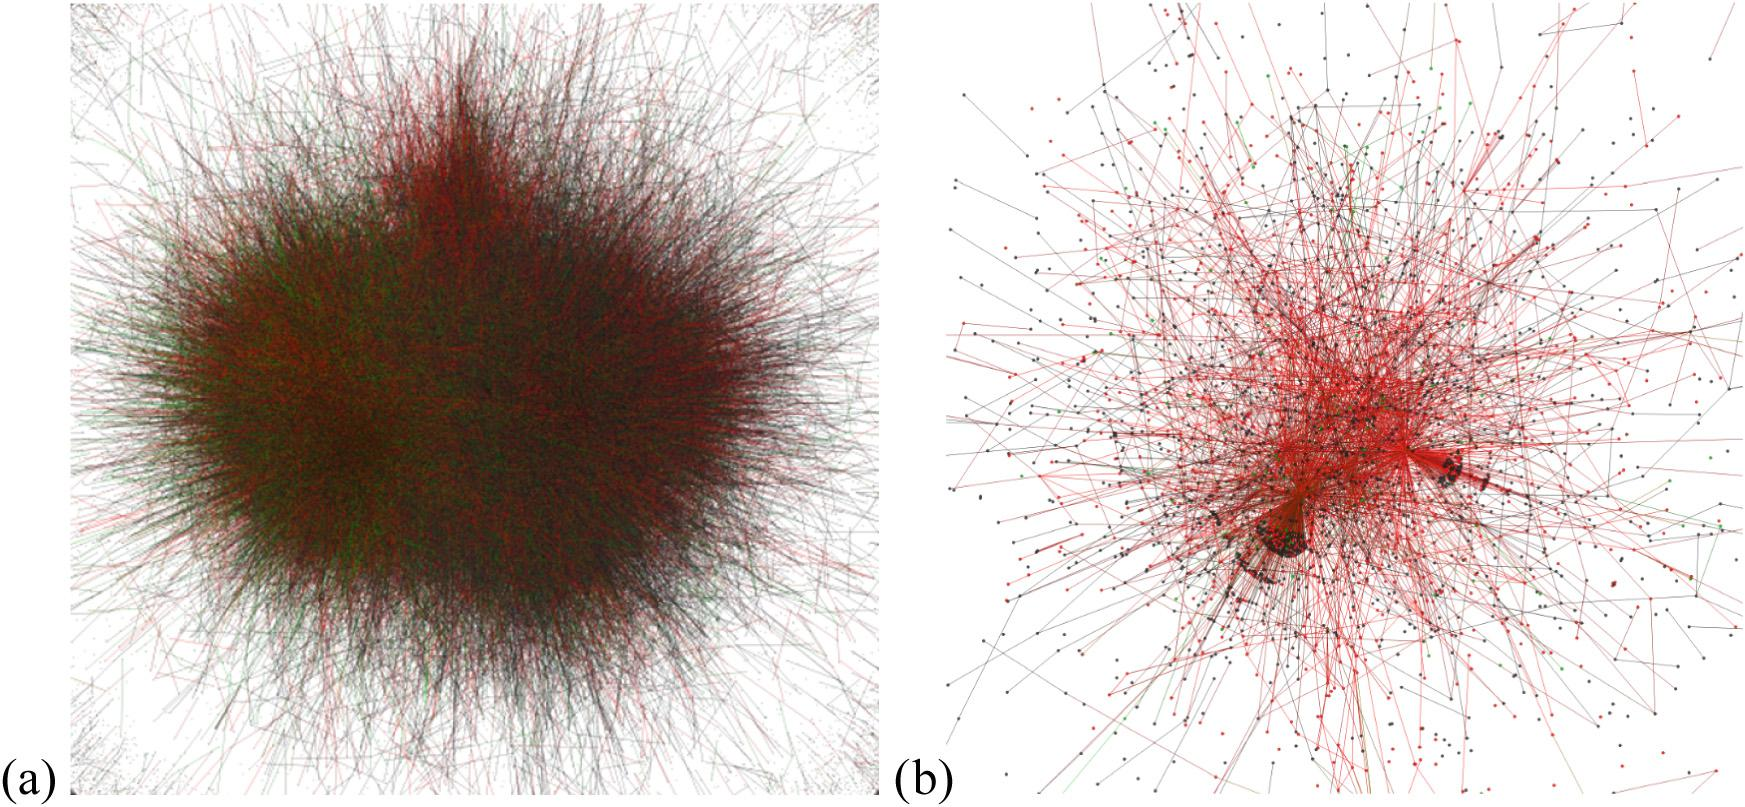
\includegraphics[scale=1.0]{overallSentimentStructure}
	}
	\caption{Sentiment-based structure: (a) \#jesuischarlie; (b) \#jenesuispascharlie (graph fragments) for the overall discussion. \textit{Green}: positive; \textit{grey}: neutral; \textit{red}: negative; \textit{mixed}: brown. (Color figure online)}\label{fig:overallSentimentStructure}
\end{figure}

\begin{figure}[ht]
	\centerfloat{
		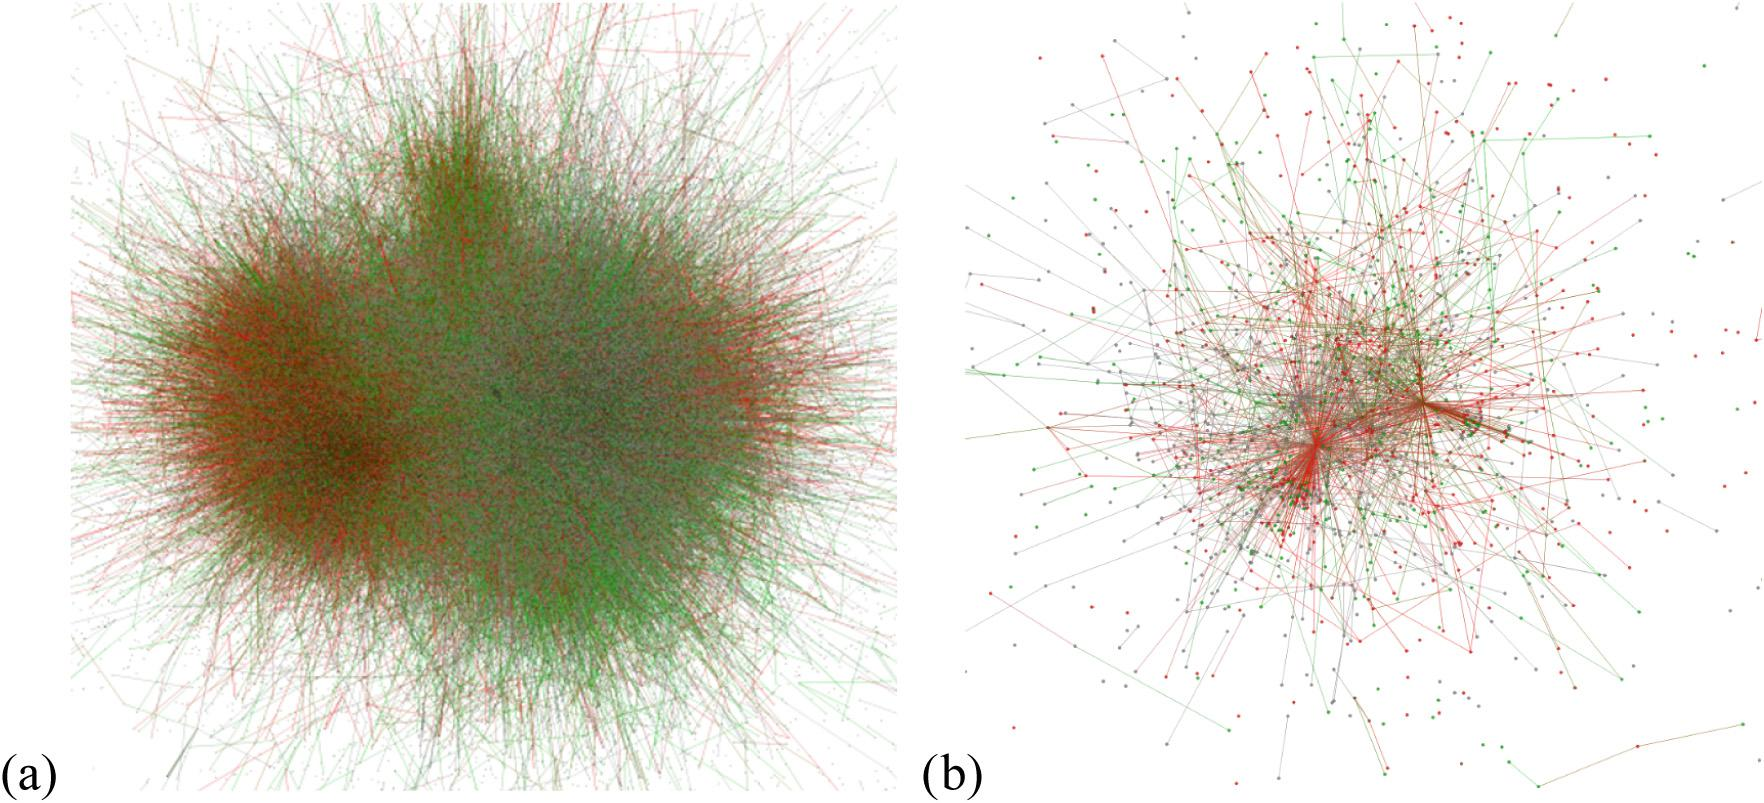
\includegraphics[scale=1.0]{francophoneSentimentStructure}
	}
	\caption{Sentiment-based structure: (a) \#jesuischarlie; (b) \#jenesuispascharlie (graph fragments) for the francophone discussion. \textit{Green}: positive; \textit{grey}: neutral; \textit{red}: negative; \textit{mixed}: brown. (Color figure online)}\label{fig:francophoneSentimentStructure}
\end{figure}

\begin{table}[ht]%
	\centering
	\caption{Number of edges inside and between clusters for both discussions}%
	\label{tab:clusterEdgesNo}% label всегда желательно идти после caption
	\begin{adjustbox}{width=1\textwidth}
		\small
		\begin{tabular}{ l  l  l  l  l  l  l }% Вертикальные полосы не используются принципиально, как и лишние горизонтальные (допускается по ГОСТ 2.105 пункт 4.4.5) % @{} позволяет прижиматься к краям
			\toprule
			User sentiment & \multicolumn{2}{l}{General discussion} & \multicolumn{2}{l}{Francophone segment} & \multicolumn{2}{l}{Francophone influencers} \\
			\cline{2-7}
			& \#jesuis & \#jenesuispas & \#jesuis & \#jenesuispas & \#jesuis & \#jenesuispas \\
			\hline
			Positive & 2.53\% & 0.25\% & 9.43\% & 3.17\% & 0.64\% & 0 \\
			Neutral & \textbf{25.03\%} & 16.29\% & 11.72\% & \textbf{22.72\%} & 0 & 0\\
			Negative & 5.19\% & \textbf{21.58\%} & 5.43\% & 9.04\% & 5.73\% & \textbf{52.38\%} \\
			Mixed & 3.85\% & 0.70\% & 5.87\% & 1.47\% & 37.58\% & 0 \\
			Between clusters & 63.40\% & 61.18\% & 67.55\% & 63.59\% & 56.06\% & 47.62\% \\
			\bottomrule
			\multicolumn{7}{@{}p{\textwidth}}{%
				\hspace*{2.5em}% абзацный отступ - требование ГОСТ 2.105
				Note. Green: the test shows the dependency of the overall discussion upon these users and authors. Yellow: the test shows that the numbers of the neutral users and emotional users correlate due to a third factor.Violet: The linkage between emotional and neutral users shows the dependency of the other direction: the higher the number of neutral tweets, the higher the number of the angry and/or compassionate tweets. That is, when the discussion is boiling itself, the number of angry users also grows without any coordinated effort.
			}\\
		\end{tabular}%
	\end{adjustbox}
\end{table}

\paragraph{4.5 Manual Analysis of Influencers’ Profiles} To answer RQ2, we have manually assessed the user profiles of the detected influencers and used descriptive statistics to see whether user status is linked to sentiment and whether most influencers, as other researchers claimed, bore negative sentiment. To address H2b, we have assessed the number of users with the four types of sentiment for both discussions, and, to assess H2a, we combined the influencers in both discussions, as their number was too small for Spearman’s rho calculations.

\subsubsection{5 Results} As stated above, we have reconstructed the web graphs based on our labeling of user sentiment (see Figs.~\cref{fig:overallSentimentStructure} and~\cref{fig:francophoneSentimentStructure}) and checked them for sentiment clusters (see Table~\cref{tab:clusterEdgesNo}).

\textit{RQ1: how sentiment affects the structure of the discussions.} Visual assessment of the graphs on Fig.~\cref{fig:francophoneSentimentStructure} shows that the discussions are divided into clusters based on user sentiment: thus, for \#jesuischarlie, a large cluster of positive/neutral interactions is surrounded by two clusters of negative/mixed sentiment, and for \#jenesuispascharlie, two distinct negative-based clusters linked to influencers lie under a greenish positive-based nebula. But the data on interactions inside and between clusters (see Table~\cref{tab:clusterEdgesNo}) show that this is a graph construction artifact. In \#jesuischarlie, users with very dif- ferent sentiment all talk to each other, rather than form closed clusters; in \#jenesuis- pascharlie, only neutral users tend to talk to each other substantially more than people in other clusters, but positive and negative sentiment anyway does not form any distinct group. Thus, H1a has to be rejected.

But at the same time we see that francophone sentiment tends to have bigger impact to the general discussions, as both graphs and the data on graph edges show that negative sentiment does tend to structure them. For \#jesuischarlie, while the negative cluster is not supported by the data on edges, it is anyway evident in the graph as a ‘flame’ at its top. While positive sentiment is ‘dissolved’ much more than in the francophone discussion in both cases, negative sentiment casts an impact on clusterizaton for \#jenesuispascharlie. Interestingly enough, negative sentiment expressed in French affects the overall discussion in the public counter-sphere, while neutral sen- timent (mostly characteristic for media and institutional talk) affects the bigger discussion. Thus, H1b is rejected for \#jesuischarlie but confirmed for \#jenesuispascharlie.

And, as we see from above, H1c on the difference between the structure of nebulae in \#jesuischarlie and \#jenesuispascharlie is confirmed for the general discussion and not for the francophone one. But here we also need to take into consideration the influencers. Here, the hypothesis is clearly confirmed, as influencers with mixed (even if not positive) sentiment are tightly grouped in \#jesuischarlie and those with negative sentiment are tightly grouped in \#jenesuispascharlie.

\textit{RQ2: what sentiment the influencers express.} As stated above, we have calculated user sentiment by assigning values as the differences between the number of tweets with positive/neutral, negative/neutral, or positive/negative sentiment; as a results, each user received a label from -- 1 to 0.56. User status was assigned as: 0 -- personal account, 1 -- individual professional account, 2 -- official account/representative, as based on manual assessment of the user accounts. For \#jesuischarlie, positive vs. neutral vs. negative was 50:19:85, and for \#jenesuispascharlie, 2:7:26. Thus, negative sentiment (fully negative, or mixed with neutral tweets, or dominating over positive tweets) was found in 55 and 74\% of the influencers, respectively. H2a is confirmed.

For H2b, we have merged the data on the influencers’ sentiment and status from the two discussions and applied Spearman’s rho metric to this dataset. We have found a weak but significant correlation between the users status and sentiment (0.209**). Also, Fig.~\cref{fig:jesuischarlieSentimentDistribution} shows sentiment distribution for \#jesuischarlie, where the cluster between -- 0.28 and 0.2 is clearly formed by institutions (mostly media). Thus, H2b is confirmed for \#jesuischarlie, while for the other hashtag the data is too scarce to tell.

\begin{figure}[ht]
	\centerfloat{
		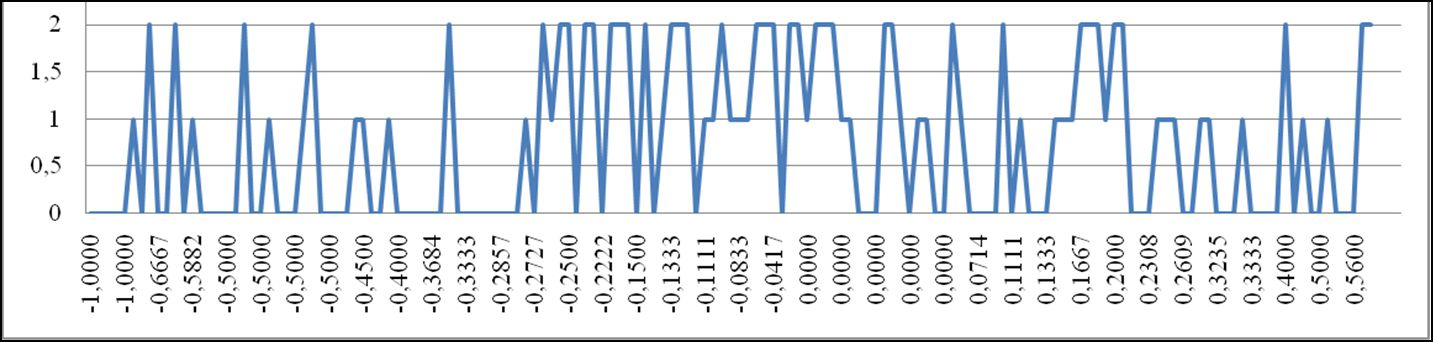
\includegraphics[scale=1.0]{jesuischarlieSentimentDistribution}
	}
	\caption{Sentiment distribution in influencers’ talk on \#jesuischarlie}\label{fig:jesuischarlieSentimentDistribution}
\end{figure}

\subsubsection{6 Discussion}

In this paper, we have assessed the user sentiment in two polar hashtagged segments of the Twitter discussion on the \textit{Charlie Hebdo} case. We have used a triangulation-based approach to detect user sentiment and have detected meaningful differences between the discussion segments.

What we have found is, first, that francophone discussions were more ‘opinion crossroads’ than echo chambers, but negative sentiment that the French users bore has cast impact upon the bigger general discussion of \#jenesuispscharlie, making this cluster a negative-leaning counter-discourse.

Second, negative inclination was especially true for the influential users, as they formed the only negative cluster between themselves and created the centers of gravity in the general discussion. We may even say that, in terms of sentiment, non-influencers have produced more balanced pictures than the influencers. Moreover, Spearman rho has shown that the more institutionalized an influencer was, the more was the probability that the account would bear positive sentiment. We have also seen that non-institutional influencers tended to polarize, while institutional accounts bore more balanced views.

Third, we have seen that the two discussion segments did differ in how the sentiment structured the discussions, but not via formation of positive and negative echo chambers within the French-speaking community but by ‘negative’ users’ talk to non-
French speakers.

Our findings on the influencers are in line with the previous research, but what we add is a possible rethinking of the level of echo chamber formation in multi-lingual discussions. To assess how the discussion is structured in terms of sentiment, one needs to look both at one language and the overall discussion. Also, we have shown that positive and negative affective hashtags do differ in sentiment, and negative hashtags, indeed, tend to bear more negative sentiment.

\section{Методы суммаризации}\label{sec:ch5/sect4}

\subsection{Global Agendas: Detection of Agenda Shifts in Cross-National Discussions Using Neural-Network Text Summarization for Twitter}\label{subsec:ch5/sec4/sub1}

\subsubsection{1. Introduction}

The spread of agendas in online media has been a focus of scholarly attention for nearly two decades \cite{McCombs2004}. However, for social media, the meaning of agendas transform; scholars discuss smaller-scale agendas and their shifts \cite{KoltsovaNagornyy} within particular online discussions, including hashtagged ones. Despite its seemingly smaller impact, in-discussion agendas may spill over to traditional media and thus press public bodies, gather support, call for action, or fuel protest. Also, affect-based discussions \cite{Papacharissi} help identify immediate popular reaction to trigger events and issues behind them.

Global-scale discussions caused by events of international relevance may evoke varying interpretations in different national contexts. And yet, evidence on cross-cultural, especially multilingual, dynamics of agendas in large-scale public discussions is still highly under-explored. In particular, we lack knowledge on whether affect-based agendas develop concurrently in various languages and to what extent they become contextualized within language-bound discussion segments, while knowing it would be relevant for elaborating quicker institutional response by, e.g., UN, EU, or other international and macro-regional organizations. Knowing how people perceive ongoing conflicts might help incorporate this knowledge into political decision-making.

Computational methods of textual analysis allow for automated detection of agendas in user talk, agenda being reinterpreted as topicality, and agenda research reconceptualized as topic detection and modeling \cite{KoltsovaNagornyy}. Earlier, we have shown that it is possible to detect pivotal points in debate on social media by assessing the saliency of detected topics within the time of discussion \cite{SmoliarovaBodrunovaYakunin}. However, classic topic models like LDA or BTM demand data processing which is often multi-run \cite{KoltcovKoltsovaNikolenko2014,BodrunovaKoltsovaKoltcov} or unfeasible due to longevity of procedures or scarcity of instruments. They also demand reading top words and inter- preting topics by human assessors, which might be tricky, and the results might be misleading. Thus, close-to-real-time agenda detection remains an unreached goal, and this often leaves potential industrial, political, and academic consumers of topicality assessment frustrated.

In this paper, we propose a method of topicality detection based on text summariza- tion produced by neural network models. And, as we aim at agenda detection in general as well as cross-language agenda shifts and comparisons, we will try to define one topic per short time slot or fixed number of user posts, to be able to follow how the agendas move. To test the method we propose, we use the Twitter discussion on the infamous \textit{Charlie Hebdo} massacre of 2015 and exploit tweets in English, French, and German that were posted under \#jesuischarlie within 24 h after the massacre (which makes thousands of tweets from all around the world).

The remainder of the paper is organized as follows. In Sect. 2, we shortly review the existing literature on agenda detection on social media and use of topic modeling and text summarization for this task. In Sect. 3, we tell of the case under scrutiny and our research questions. In Sect. 4, we describe the methodology, formation of sub-datasets and their processing, as well as quality checks by application of sentiment analysis. In Sect. 5, we provide the results of text summarization and assess the cross-language agenda shifts. In Sect. 6, we discuss the findings and reflect on methodological limitations of our research.

\subsubsection{2. Agenda Detection vs. Topicality Detection: Current Approaches}

\paragraph{2.1 Public Agendas on Social Media: Do They Matter?}
As stated above, agendas in online media have been a focus of scholarly research for nearly two decades \cite{McCombs,KimLee}. From the very beginning, the major attention has been put to how agendas of online media, then blogs, and then social media (‘mediated public agendas’) built into the exiting agenda-setting infrastructures. Reverse and cross-platform agenda-setting, as well as other types of interplay between older and newer agenda-setting actors, were suggested. The focus on ‘who sets the agendas’, however, provoked a certain inertia in understanding of the nature of public agendas and processes of their formation – not only regarding the topics that people discuss but also the features of ‘agenda building blocks’ and discursive localization of agendas.

Gradually, computational research has entered agenda studies \cite{RussellNeumanGuggenheimMoJang,Guo,KoltsovaBodrunova}, and, following the works on methods of textual analysis, ‘public agendas’ were in several influential works reconceptualized via topicality and explored with the help of topic modeling and similar techniques \cite{KoltsovaKoltcov}, thanks to the capability of probabilistic text clustering to capture the themes in large text corpora.

These studies, though, had a double-edged impact upon how we understand public agendas that emerge on social media platforms. On one hand, topicality studies have highlighted the importance of in-discussion topicality and agenda shifts, while, earlier, agendas were seen as belonging to the highest level of content generalization, e.g., the whole content of public debate. On the other hand, the scholarly attention massively moved to methodological aspects of topic detection, and, due to early-stage methodological limitations, the topics could not be discovered in real time and were substituted by the post-factum evaluations. Later works have tackled this problem in various ways (see below), but, till today, we lack approaches that would be relatively easy solutions for assessment of agenda shifts in near-to-real time.

This is especially relevant for the areas where cross-country comparisons are neces- sary. The 2020–2021 COVID-19 pandemic has shown how crucially important it was to trace local public reactions to global-scale events and issues; earlier, European migra- tion crisis, the 2008–2209 global recession, and globalized military conflicts like the one in Syria have demanded for advancement of methodologies of agenda detection in multilingual online environments.

We cannot help mentioning, of course, that there is also a substantial corpus of academic and analytical writing that emphasizes trivial nature and unimportance of public agendas \cite{Fuchs,MartinGrub}. Indeed, empirical research suggests provides mixed evidence on whether social media and microblogs can well play an indicator role in terms of agenda shifts. Partly, it is due to social non-representativity of platform use. But it is also true because the Twitter population has its own substantial agendas, as compared to traditional media and survey results \cite{PoseggaJungherr}, while Twitter agendas of politicians my closely correlate with their offline deliberative agendas \cite{CasasMorar}. This proves again that ‘patterns of societal activity observed through the lens of Twitter research are... dependent on a range of additional variables’ and need to be assessed case-to-case \cite[p.~4]{BrunsStieglitz}.

\paragraph{2.2 Automated Agenda Detection}
Automated means of topicality detection has been a rapidly growing area of research, and its relations with agenda studies, being truly multi-faceted, have not escaped certain meaningful limitations.

\textbf{Agendas vs. Topics: The Issue of Simultaneity.} One of the biggest limitations of topic modeling for agenda detection is that the models work with text corpora as if the texts they contain were created simultaneously; the posting time is not calculated in. Thus, in classic models, it is impossible to see how agendas (topic diversity and substance) change in time. However, tracking the agenda shifts is basically the essential task of agenda setting studies. Several studies have used Granger causality testing and vector autoregressions (VAR) to detect agenda dependence either across platforms \cite{RussellNeumanGuggenheimMoJang} or across actor groups on Twitter \cite{BarberaCasasNagler}. Both studies, even if successfully detected dependencies in cross-platform impact, issue attention, and prediction by groups of Twitter users, did not focus on agendas themselves and how they evolved, seeing agenda issues as constant. Another work \cite{TsurCalacciLazer} assessed political spin and party discipline in the US Democrat and Republican tweets with the help of topic modeling, autoregressive distributed-lag modeling, and n-gram assessment; the authors have detected time lags between the party agendas and differences in ‘discourse ownership’ in terms of lexicons; the authors also used data slicing into varying time spans to detect agenda cycles. But the very agendas and time shifts between them were not discussed.

This, in effect, does not allow us to learn about \textit{the pace of public agendas} on social media -- how quickly they change, i.e., what time or number of posts is needed to significantly shift them. While media are still, even if to a much-decreased extent, subjected to their news production cycle which takes hours and days, social media can potentially shift agendas in minutes during (and within!) outbursts of public reaction.

\textbf{Topic Evolution Studies.} Scholars have tried to overcome this limitation by developing topic evolution studies -- the area of research that models emergent and evolving topics within social media data. But the general intention of this group of studies is looking at how the identified topics evolve in time within themselves (see, e.g., \cite{AlamRyuLee,ZhangMaoLin} and also \cite{ZhangMaoZeng} for short texts), including how they evolve all in parallel, not how the public shifts from one dominant theme to another. This idea, though, has been amplified in various ways that come closer to the idea of representing agendas. Thus, by focusing on both evolving themes and emergent topics, researchers have introduced emergence regularization for topic detection, which may potentially be used to detect emerging agendas \cite{SahaSindhwani}, as well as metrics for measuring novelty and fading of topics \cite{HuangPengWang}. However, the focus on emergent topics still blurs from view the detection of the \textit{main} topics in each period of time.

Several studies \cite{DengCaiZhang}, including ours \cite{SmoliarovaBodrunovaYakunin}, have focused on relative saliency of the topics found throughout the dataset. By such studies, we can see \textit{what} (of the topics discovered) is discussed more and \textit{when}; but we do not see \textit{how} the themes look like and what their substantial features are, which is essential in agenda studies. Another pack of research papers focusses on topic-sentiment relation over time (for a short review and original results, see \cite{DermoucheVelcinKhouas}). In this work, again, the authors receive results within the pre-discovered topics.

Thus, paradoxically, in the works dedicated to modeling topic evolution, we do not see the evolving topics themselves, only the model on the whole and its quality. The same goes for trending topics detection \cite{WangAgichteinBenzi}: except for Twitter itself, we practically do not see how exactly the new trending topics look and how they are thematically or otherwise connected/different from the existing topics.

This is why it remains important to look at what people actually talk about in dynamics and, moreover, learn it in the quickest possible way.

\textbf{Cross-Language Agenda in Online Discussions: Putting Topics in Context.} Another issue in social media agenda studies is the (alleged) global character of the discussions and, thus, the extent to which the agendas related to the same issues or events and discussed in various language-bound segments of discussions get contextualized and ‘nationalized.’

First of all, it needs to be stated that the discussions that are seen as global by conventional wisdom demonstrate, in reality, high inequalities in language (and, thus, country, culture, and values) representation. This is true for the case we assess further in the text, namely the discussion hashtagged \#jesuischarlie of 2015 \cite{BodrunovaSmoliarovaBlekanov}. However, such discussions are involving enough cross-nationally to pose questions of whether the topicality and agendas that emerge can be compared across countries and what their substance is in comparative perspective; how and via what means they get contextualized in national discussion segments; and whether there are time lags between the rising waves of compassion, shock, or outrage.

Till today, cross-country studies in general social media remain relatively rare \cite{BodrunovaBlekanovSmoliarova}. At the same time, the issue of context as the discussion definer is one of those of acute importance \cite{Bodrunova,Bodrunova2020} -- and, despite this, remains a significant research gap. Context for Twitter studies is understood in varying ways: it is defined via the hashtag distribution/hashtag clusters \cite{AlamRyuLee}, in some cases, Twitter itself is seen as provider of social context for interpreting news agendas in traditional media \cite{KalyanamMantrachSaezTrumper}. The closest to the agenda-tracking idea seems to be the evolutionary clustering approach called Recurrent Chinese Restaurant Process (RCRP) \cite{AhmedXing}, as it has been developed to involve contextual variability by capturing temporal dynamics and local semantic sequential dependencies \cite{LuTanLi}. The only problem with this method is that it demands complicated layer-introduction procedures.

Thus, we are looking for a method that would allow for tracking the current (or immediately previous) agenda/topicality of online discussions that would allow for showing the agenda in a quick enough and accessible way in comparative cross-language perspective.

\paragraph{2.3 Text Summarization in Agenda Detection Studies}

For resolving this task, we suggest to use another method of topic formulation, which is text summarization. Successfully used in computational studies of text corpora, text sum- marization allows to ‘summarize the text documents in order to obtain a brief overview of a large text document or a set of documents on a topic’ \cite[p.~4]{AggarwalZhai} and ‘to produce a concise and fluent summary conveying the key information in the input’ \cite[p.~44]{NenkovaMcKeown}. Summarizations may be of extractive and abstractive nature; in the latter case, the machine provides a textual summary of a text (sub-)corpus that may contain words that were not found in the initial data. They may also be indicative (providing a very brief indication summary) and informative (providing more information on the text); and be executed over single or multiple documents  \cite{NenkovaMcKeown}. Previous research also shows that summarization may depend on the text subject and the nature of the dataset (e.g. news texts, documents, or social media posts) \cite{TasKiyani}.

Today, advanced text summarization studies are conducted with the use of neural networks (for an early account, see \cite{FerreiraFreitasDeSouza}; for a later one on abstractive summarization, \cite{Kaikhah}). Neural networks are employed for both extractive \cite{NallapatiZhouGulcehreXiang} and abstractive summarization \cite{CelisKeswani} for Twitter. Earlier, several successful instruments for Twitter text summarization have been proposed, like TweetMotif \cite{LiZhang}. Later models employ BERT \cite{CelisKeswani} and USE \cite{MottaghiniaFeiziDerakhshiFarzinvash} architectures. In 2019--2020, new transformer-based architectures such as Longformer \cite{AsgariChenaghluNikzadKhasmakhiMinaee} and t5 \cite{BeltagyPetersCohan}, have been proposed and tested; we see them as most suitable for our tasks.

In our research, we use the existing text summarization models; their quality has been tested multiple times. This is why we do not use traditional quality metrics assuming that the models produce sustainable results. However, we provide additional checks oriented to our research questions and use sentiment analysis for detecting the quality of summarization. Even if, as a rule, sentiment analysis is used in combination with summarization in order to reach substantial goals, there is also evidence that sentiment detection can be used as a quality indicator for topics \cite{RaffelShazeerRoberts} and summarizations.

\subsubsection{3. Research Questions and the Datasets}

\paragraph{3.1 The Case Under Scrutiny and the Language-Based Datasets}
Thus, in this study, we focus on detecting agendas and agenda shifts in various language-bound segments within one globalized discussion. For that, we use the dataset we have collected in 2015 by the hashtag \#jesuischarlie that gathered much of the user reaction to the Charlie Hebdo massacre in Paris, France. The dataset was collected using our own patented web crawler \cite{BodrunovaBlekanovKukarkin}, comprised the three first days of the discussion and, after cleaning and preprocessing, contained 420,080 tweets.

This dataset of over five years ago was chosen, as it was much less bot-infested than today’s data. It contained a discussion that, to a large extent, reproduced the language structure of Twitter itself \cite{BlekanovSergeevMartynenko}, with circa 50\% of posts being in English \cite{BodrunovaSmoliarovaBlekanov}.

This dataset allows for looking at two languages -- English and French -- as similarly dense, which makes it possible to juxtapose the ‘global’ (Eng-lang) and ‘local’ (Francophone) reaction of the Twitter populace. We have also chosen a third language, in order to see how the discussion differs in a much looser discussion segment. We have chosen German based on the number of tweets on main languages of the discussion (see Fig.~\cref{fig:charlieHebdoLanguageDistribution} and Table~\cref{tab:projectSubDatasets}). The language of tweets was detected by using the FastText algorithm \cite{MocanuBaronchelliPerra}.

As a result, we have received three datasets: English (213,558 tweets), French (133,671 tweets), and German (7,430 tweets).

\begin{figure}[ht]
	\centerfloat{
		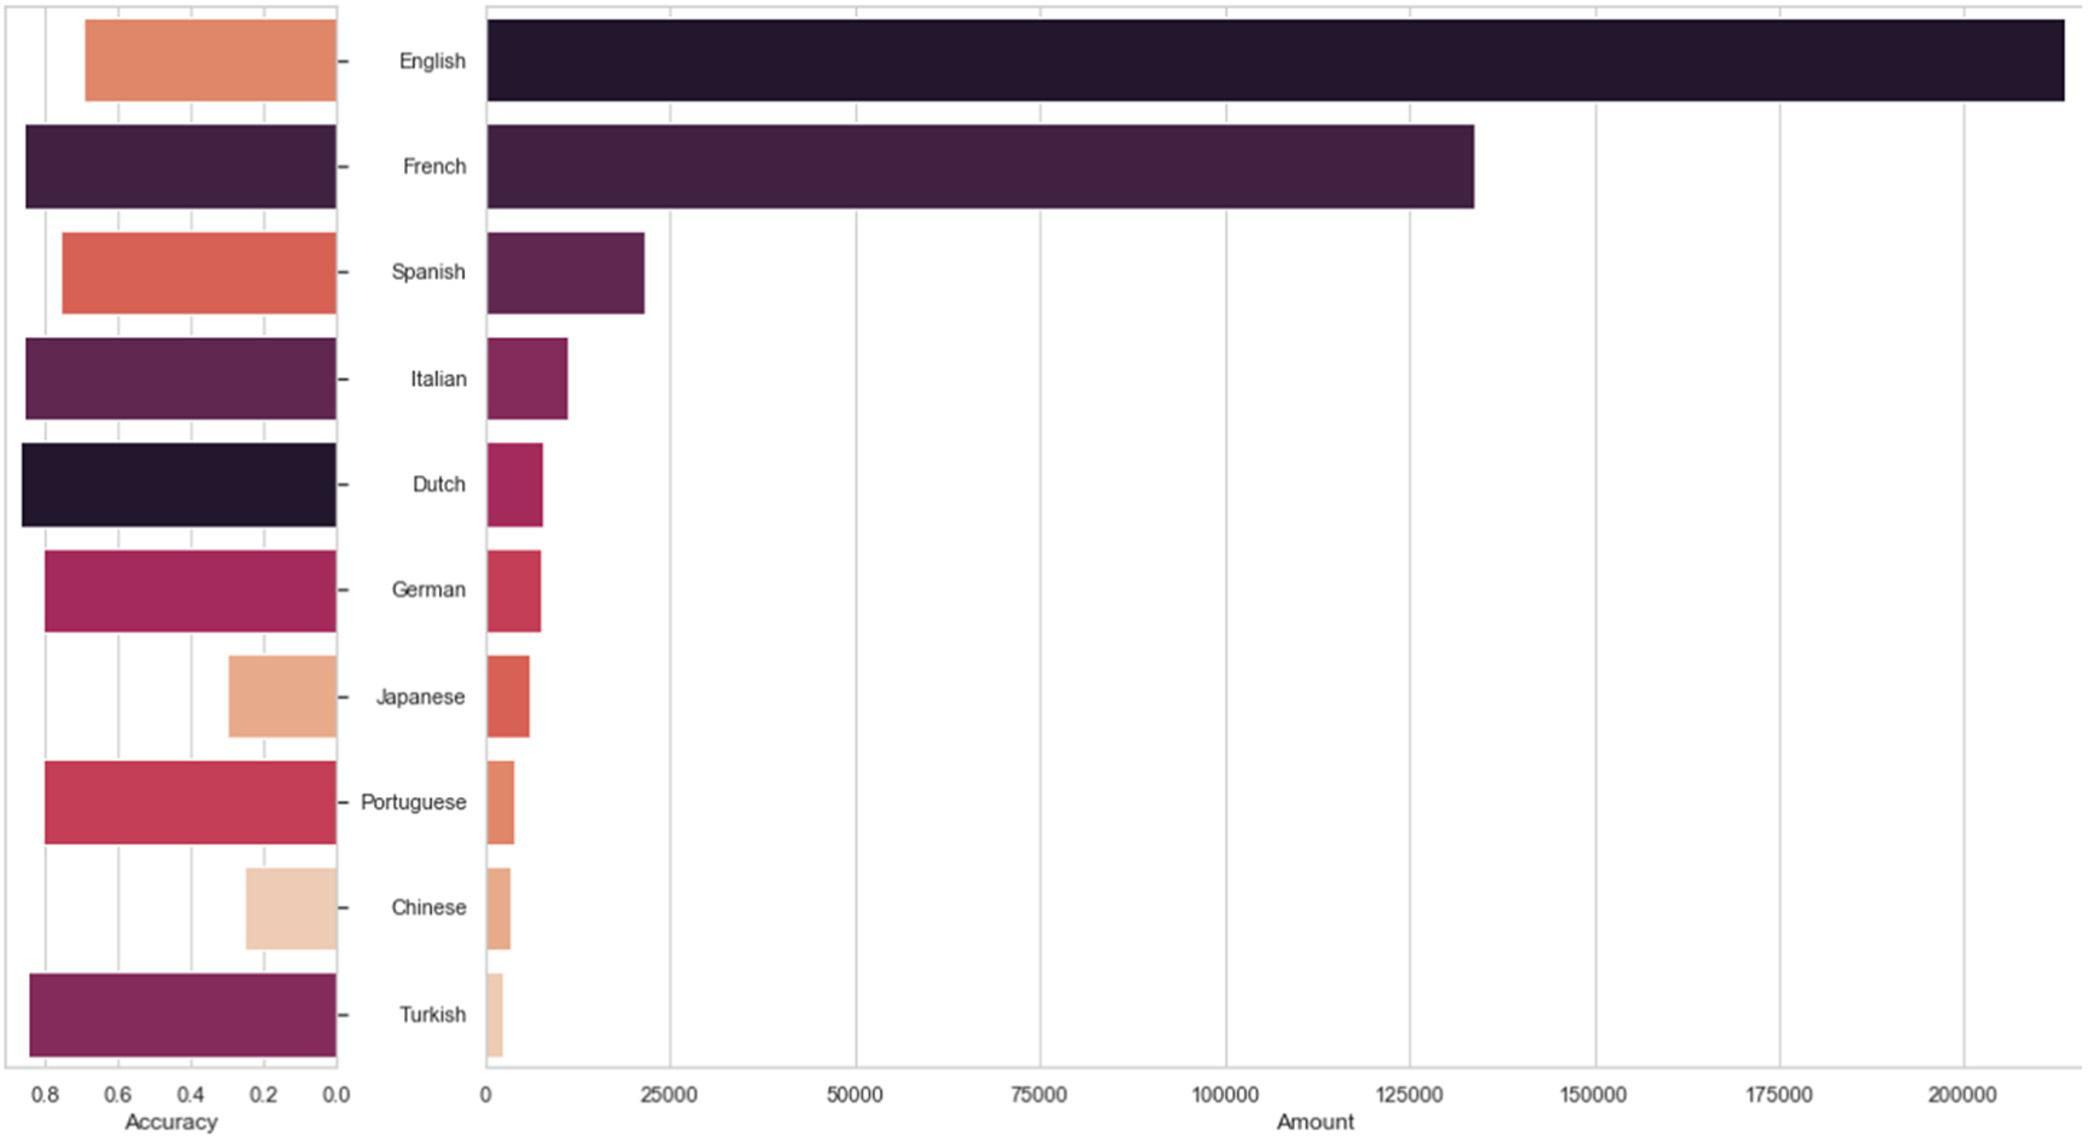
\includegraphics[scale=1.0]{charlieHebdoLanguageDistribution}
	}
	\caption{Language distribution in the \#jesuischarlie discussion.}\label{fig:charlieHebdoLanguageDistribution}
\end{figure}

\begin{table} [htbp]%
	\centering
	\caption{Sub-datasets of the project.}%
	\label{tab:projectSubDatasets}% label всегда желательно идти после caption
	\renewcommand{\arraystretch}{1.5}%% Увеличение расстояния между рядами, для улучшения восприятия.
	\begin{SingleSpace}
		\begin{tabulary}{\textwidth}{@{}>{\zz}L >{\zz}L >{\zz}L >{\zz}L@{}} %Вертикальные полосы не используются принципиально, как и лишние горизонтальные (допускается по ГОСТ 2.105 пункт 4.4.5) % @{} позволяет прижиматься к краям
			\toprule     %%% верхняя линейка
			Language & Accuracy & N of tweets & \textit{\%} of total\\
			\midrule %%% тонкий разделитель. Отделяет названия столбцов. Обязателен по ГОСТ 2.105 пункт 4.4.5
			English & 0.6961355805397034 & 213,558 & 0.51\\
			French & 0.8610345721244812 & 133,671 & 0.32\\
			Spanish & 0.7578563690185547 & 21,604 & 0.05 \\
			Italian & 0.8599529266357422 & 11,251 & 0.027 \\
			Dutch & 0.8691623210906982 & 7,699 & 0.018 \\
			German & 0.8065633773803711 & 7,430 & 0.018 \\
			Japanese & 0.30159252882003784 & 5,946 & 0.014 \\
			Portuguese & 0.8060423731803894 & 3,874 & 0.009 \\
			Chinese & 0.2554042339324951 & 3,423 & 0.008 \\
			Turkish & 0.8499038219451904 & 2,261 & 0.005 \\
			\bottomrule %%% нижняя линейка
		\end{tabulary}%
	\end{SingleSpace}
\end{table}

\paragraph{3.2 Research Questions}
Our research questions relate to both methodology of text summarization and to the substance of our study of agenda shifts.

\paragraph{RQ1. How well does the neural-network-based text summarization capture agendas from tweets in three languages?}

\begin{itemize}
	\item H1. Summarized sentiment of the tweet conglomerates is reflected by the sentiment of summarizations.
\end{itemize}

\paragraph{RQ2. Do agendas develop simultaneously in the global and local segments of a Twitter discussion?}

\begin{itemize}
	\item H2. Agendas shift simultaneously (within very short timing) in the local and global discussion segments. There is no detectable time lag between the same agendas in the local and global segments of discussions if they develop with comparable density.
	\item H3. In looser discussion segments, agendas shift more radically thematically.
\end{itemize}

\paragraph{RQ3. Are Twitter agendas within one discussion get contextualized in various language segments?}

\begin{itemize}
	\item H4. Text summarizations represent local context in a negligible percentage of cases (less than 5\%) for all the three cases.
\end{itemize}

\subsubsection{4. Methods and Data Processing}

\paragraph{4.1 Application of Text Summarization}

\textbf{The Choice of Summarization Models.} Basedonthelatestliterature,wehavechosen two models mentioned above, namely Longformer and t5, for text summarization.

Pretrained Longformer model was used to summarize subset in the English language. Longformer is a language model with a unique attention mechanism that scales linearly with sequence length (as opposed to the quadratic scaling of traditional models), making it easy to process documents of thousands of tokens or longer \cite{AsgariChenaghluNikzadKhasmakhiMinaee}. The resulting summarization is obtained using the longformer-large-4096 pretrained model.

For French and German, t5 model was used with t5-base-fr-sum-cnndm and mt5-small-german-finetune-mlsum pretrained models, respectively. T5 is an encoder-decoder model and converts all NLP problems into a text-to-text format. T5 is an encoder-decoder model and converts all NLP problems into a text-to-text format. While providing a very general and well-built structure with unified framework for a variety of NLP tasks, authors achieve state-of-the-art results on many benchmarks covering summarization, question answering, text classification, and more. T5 uses a standard encoder-decoder Transformer with a baseline model designed so that the encoder and decoder are each similar in size and configuration to a BERT. Specifically, both the encoder and decoder consist of 12 blocks (each block comprising self-attention, optional encoder-decoder attention, and a feed-forward network with ReLU nonlinearity) \cite{BeltagyPetersCohan}.

\textbf{The Choice of Increment.} Aswehavestatedabove,threelanguageswerechosenbased on the models’ accessibility, peer review potential, identification quality, and the sample structure and volume.

The most problematic issue for us was the choice of the ‘step’ for agenda shifts, or the increment, that would fit both our RQs and the tweet distribution. And it was not the timing itself. The matter was that both summarization models had a limitation, as they worked best with certain number of texts. To find the optimal number of tweets for summarization, we have constructed diagrams of tweet distribution in time in each sub-set. We have constructed them for 1-h, 3-h, and 6-h increments (see Fig.~\cref{fig:frenchTweetDistribution},~\cref{fig:englishTweetDistribution}, and~\cref{fig:germanTweetDistribution} for 1-h increments for French, English, and German, respectively).

\begin{figure}[ht]
	\centerfloat{
		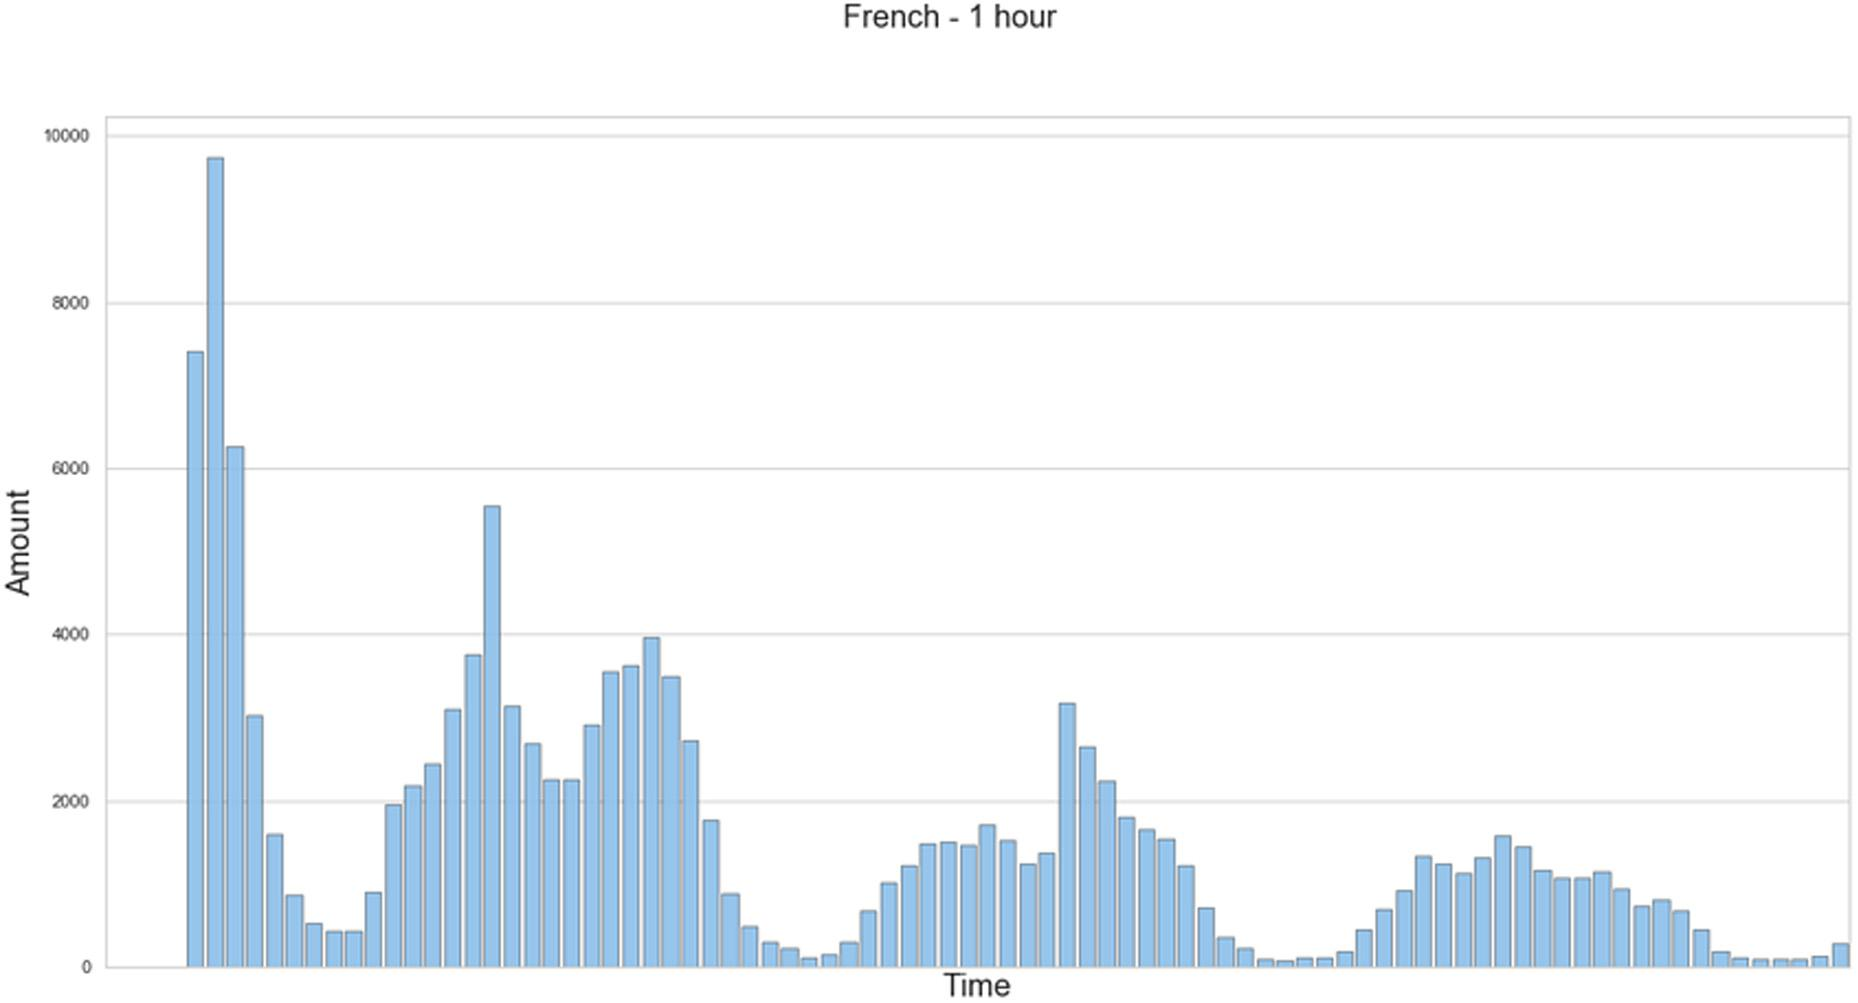
\includegraphics[scale=1.0]{frenchTweetDistribution}
	}
	\caption{The French-language tweet distribution, 1-h increment.}\label{fig:frenchTweetDistribution}
\end{figure}

\begin{figure}[ht]
	\centerfloat{
		\includegraphics[scale=1.0]{englishTweetDistribution}
	}
	\caption{The English-language tweet distribution, 1-h increment.}\label{fig:englishTweetDistribution}
\end{figure}

\begin{figure}[ht]
	\centerfloat{
		\includegraphics[scale=1.0]{germanTweetDistribution}
	}
	\caption{The German-language tweet distribution, 1-h increment.}\label{fig:germanTweetDistribution}
\end{figure}

Our decision-making in choosing the increment for summarization was, in the end, based on two circumstances. First, the limitation of the model showed circa 300 tweets to be the optimal number to be summarized; second, the German model as the most sparce showed that 300 tweets would comprise 1 to 2 h in the most sparce case, which suits our goal. But, to make the pace comparable, we should have either used an increment based on tweets or the one based on hours.
We have opted for the number of tweets, even if it looks counter-intuitive. This was because: (1) the hourly number of tweets varied highly in 24-h cycles, and thus the summarizations would be incomparable; (2) the 300-tweet samples allow for a more fine-grained study, and several 300-tweet summarizations may reflect an hourly time span; but an hourly time span that comprises several thousand tweets might be too general and non-informative.

Thus, we have chosen 300-tweet increments for summarization. They allow to trace hourly dynamics of agenda for the German case (daytime) and for more fine-grained gaze into the English and French cases.

\textbf{Summarization Results.} However, the models we have received were not satisfactory at the first trials. While the English-language one was clearly understandable, with only rare non-comprehensible inclusions, the German and French versions returned understandable but broken sentences with loose endings (for examples, see Table~\cref{tab:threeLanguagesSummarizations}, marked in bold). Additional runs did not bring better results; later, we will check the model with other datasets to find out why the sentences were broken.

\begin{table}[ht]%
	\caption{Text summarizations: examples for the three languages.}%
	\label{tab:threeLanguagesSummarizations}% label всегда желательно идти после caption
	\renewcommand{\arraystretch}{1.6}%% Увеличение расстояния между рядами, для улучшения восприятия.
	\def\tabularxcolumn#1{m{#1}}
	\begin{tabularx}{\textwidth}{@{}>{\raggedleft}X >{\raggedleft}X >{\raggedleft\arraybackslash}X@{}}% Вертикальные полосы не используются принципиально, как и лишние горизонтальные (допускается по ГОСТ 2.105 пункт 4.4.5) % @{} позволяет прижиматься к краям
		\toprule     %%% верхняя линейка
		English & French & German \\
		\midrule %%% тонкий разделитель. Отделяет названия столбцов. Обязателен по ГОСТ 2.105 пункт 4.4.5
		2015–01-07 12:26:00 the terrorist attack on the offices of the satirical magazine Charlie Hebdo has left 12 dead & 2015–01-07 12:03:00 Le mardi, à Bruxelles, il y a une minute de silence \textbf{pour} & 2015–01-07 12:24:00 RT und klingt nicht nur ähnlich.. \textbf{Du caricaturiste haitien Bousiko}\\
		2015–01-07 12:31:00 this is a tribute to the 12 people who were killed in the attack on the satirical magazine \textbf{@xmath0} & 2015–01-07 12:28:00 Le hashtag \#suischarlie est le plus utilisé de toute l’histoire\textbf{de} & 2015–01-07 15:20:00 Anschlag auf Satire-Zeitung: Dieter Nuhr rettet sich in Bunker\\
		2015–01-07 12:33:00 the attack on the offices of the satirical magazine Charlie Hebdo has left 12 people dead and 12 others wounded & 2015–01-07 12:29:00 Le dessin de Cabu s’éteint en hommage aux 12 & 2015–01-07 21:17:00 Der Pariser Anschlag ist auch auf Facebook und Twitter das grosse Thema. Irr\\
		2015–01-07 12:34:00 this is a tribute to the 12 people killed in the terrorist attack on the satirical magazine on the 12th of january 2015 & 2015–01-07 12:30:00 Charlie Hebdo est mort dimanche à Brest. \textbf{Les kiosques} & 2015–01-07 23:52:00 Hollande hat in der Hand, ob Frankreichs Demokratie Anschlag überlebt-\textbf{zu}\\
		2015–01-07 12:36:00 we are all Charlie & 2015–01-07 12:32:00 Nouveau: hommage à Stéphane Charbonnier \textbf{et} & 2015–01-08 01:27:00 Cartoonist Jean Jullien:. "Wir trauern um Frankreichs \textbf{bedeuten}\\
		\bottomrule %%% нижняя линейка
	\end{tabularx}%
\end{table}

\paragraph{4.2 Quality Assessment of Summarization by Sentiment Detection}

Given that the models, despite their high reputation, have provided results that were not fully satisfactory, we have introduced additional checks of the model quality. As we mentioned above, we have used sentiment detection to construct a quality metric. A BERT model \cite{JoulinGraveBojanowski} pretrained for multilingual sentiment analysis was used for each summarization to analyze summaries in the context of generalised sentiment.

In general, the idea was to compare sentiment of the original tweet samples to that of the respective summarizations. First, we have compared the mean sentiment of 300 tweets to the sentiment of the summarizations. We have seen that, in the overwhelming majority of cases, the sentiment of the 300 tweet samples tends to neutral (see Fig.~\cref{fig:englishMeanSentiment} for English). This is why we have introduced another way of measurement that aimed at highlighting the positive/negative difference in the samples. We have labeled the tweets: ‘negative’ -- \(0 \le k < 0.4\); ‘neutral’ -- \(0.4 \le k < 0.6\); ‘positive’ -- \(0.6 \le k \le 1\). Then we eliminated the neutral tweets and calculated the difference between the positive and negative tweets, to see which sentiment dominated in the sample. We compared the sentiment of the samples to that of the summarizations (see Fig.~\cref{fig:englishPosNegDiff},~\cref{fig:frenchPosNegDiff}, and~\cref{fig:germanPosNegDiff} for English, French, and German, respectively).

\begin{figure}[ht]
	\centerfloat{
		\includegraphics[scale=1.0]{englishMeanSentiment}
	}
	\caption{Representation of sentiment distribution in time, the English sub-dataset, mean sent iment score: tweet samples, blue; summarizations, red. (Color figure online)}\label{fig:englishMeanSentiment}
\end{figure}

\begin{figure}[ht]
	\centerfloat{
		\includegraphics[scale=1.0]{englishPosNegDiff}
	}
	\caption{Representation of sentiment distribution in time, the English sub-dataset, positive/negative difference, blue; summarizations, red. (Color figure online)}\label{fig:englishPosNegDiff}
\end{figure}

\begin{figure}[ht]
	\centerfloat{
		\includegraphics[scale=1.0]{frenchPosNegDiff}
	}
	\caption{Representation of sentiment distribution in time, the French sub-dataset, positive/negative difference, blue; summarizations, red. (Color figure online)}\label{fig:frenchPosNegDiff}
\end{figure}

\begin{figure}[ht]
	\centerfloat{
		\includegraphics[scale=1.0]{germanPosNegDiff}
	}
	\caption{Representation of sentiment distribution in time, the German sub-dataset, positive/negative difference, blue; summarizations, red. (Color figure online)}\label{fig:germanPosNegDiff}
\end{figure}

By manual assessment of over 100 tweet samples vs. summarizations, we have established that good correspondence in the pair ‘sample -- summarization’ is when the distance between them is circa 0.25. To measure the quality of the model, we calculated the percentage of the pairs ‘sample -- summarization’ with the distances of 0.25 or less for both types of sentiment measurement. The received values are shown in Table~\cref{tab:modelQualityMeasurements}.

\begin{table}[ht]%
	\centering
	\caption{Sub-datasets of the project.}%
	\label{tab:modelQualityMeasurements}% label всегда желательно идти после caption
		\small
		\begin{tabular}{ c  c  c }% Вертикальные полосы не используются принципиально, как и лишние горизонтальные (допускается по ГОСТ 2.105 пункт 4.4.5) % @{} позволяет прижиматься к краям
			\toprule     %%% верхняя линейка
			Language & Metric by average score & Metric by difference score \\
			\midrule %%% тонкий разделитель. Отделяет названия столбцов. Обязателен по ГОСТ 2.105 пункт 4.4.5
			English & 27\% & 51\%\\
			French & 69\% & 61\%\\
			German & 58\% & 48\% \\
			\bottomrule %%% нижняя линейка
		\end{tabular}%
\end{table}

Our measurements show that, despite the broken sentences in French and German, the sentiment scores for these models are relatively high. The graphs show, though, that the ‘movement’ of summarizations does not follow the positive/negative dynamics of tweet samples. Thus, in future, more manual assessment needs to be done for short-text data to understand how well the summaries capture the tone of public speak in a particular moment.

\subsubsection{5. Results: Global Interpretational Agendas vs. Local News Agendas in a Global Twitter Discussion}

\paragraph{5.1 RQ1: Quality of Representation of Agendas by Tweet Summaries}
As we have seen from Table~\cref{tab:modelQualityMeasurements}, the models work moderately well in terms of overall performance, when sentiment is measured as the difference between positive and negative tweets. However, when we have given a look to the original texts vs. summaries, we have noticed that the English ones summarized the user sentiment and contents much better. Thus, in our future work, we will use Longformer and train it to be used for German and French. As for now, H1 may be partly proven but needs more studies.


The two other RQs are based on our additional coding of the summarizations (see Table~\cref{tab:subDatasetAgendas}). We coded them for being (1) news or opinion/issue and (2) local/global. Combining (1) and (2) and stating keywords for the issues found, we have received the agendas and could judge their nature and shifts.

\begin{longtblr}[
	caption = {Agendas in the sub-datasets, first 50 summarizations of January 07 (English and French)/full list (German)},
	label = {tab:subDatasetAgendas},
	remark{\hspace*{2.5em}Note} = {Highlighted: local; red: new; grey: news; black: previously mentioned issues.},
	]{
		colspec = {XXXXXX}, 
		width = 1.0\linewidth,
		rowhead = 1,
	} 
			\toprule     %%% верхняя линейка
			Time & English & Time & French & Date time & German \\
			\midrule %%% тонкий разделитель. Отделяет названия столбцов. Обязателен по ГОСТ 2.105 пункт 4.4.5
			8:51 & news & 12:03 & news & 07.01 12:24 & uninterpretable \\
			12:26 & news & 12:25 & \textbf{news: local} & 07.01 13:20 & media \\
			12:28 & freedom of expression & 12:26 & tribute & 07.01 14:10 & news: French\\
			12:29 & freedom of expression & 12:28 & hashtag & 07.01 15:20 & \textbf{news: local}\\
			12:31 & news & 12:29 & \textbf{tribute: local} & 07.01 21:17 & hashtag\\
			12:33 & news & 12:30 & news & 07.01 23:52 & Francois Hollande\\
			12:34 & news & 12:32 & \textbf{news: local} & 08.01 1:27 & mourning: French \\
			12:36 & solidarity & 12:33 & news & 08.01 2:52 & solidarity: French \\
			12:38 & news & 12:35 & news & 08.01 4:06 & opinion \\
			12:40 & news & 12:36 & \textbf{news: local} & 08.01 5:45 & mourning: global \\
			12:42 & deadliest in history & 12:38 & \textbf{news: local} & 08.01 7:36 & news: French \\
			12:43 & news & 12:39 & \textbf{news: local} & 08.01 9:09 & news: French \\
			12:45 & religion & 12:40 & tribute & 08.01 10:26 & media \\
			12:47 & solidarity & 12:42 & media & 08.01 11:57 & opinion \\
			12:48 & pacifism & 12:43 & news & 08.01 13:58 & opinion \\
			12:50 & freedom of expression & 12:45 & \textbf{tribute: local} & 08.01 22:55 & Mohammad cartoons \\
			12:51 & freedom of expression & 12:46 & armistice over ChEbdo & 09.01 1:43 & opinion \\
			12:53 & freedom of expression & 12:47 & \textbf{news: local} & 09.01 4:32 & solidarity \\
			12:55 & impact & 12:49 & \textbf{France is rising} & 09.01 6:51 & opinion \\
			12:57 & news & 12:50 & news & 09.01 8:58 & solidarity \\
			12:59 & news & 12:52 & \textbf{news: local} & 09.01 12:06 & war on terrorism \\
			13:00 & freedom of expression & 12:53 & news & 10.01 0:44 & news: French \\
			13:02 & freedom of expression & 12:55 & \textbf{solidarity: local} & 10.01 5:52 & opinion \\
			13:04 & mourning & 12:56 & Fidel Castro & 10.01 13:36 & mourning: French \\
			13:06 & news & 12:58 & \textbf{Death of the Republic} & & \\
			13:08 & solidarity & 13:00 & \textbf{news: local} & & \\ 
			13:10 & freedom of expression & 13:01 & \textbf{news: local} & & \\
			13:12 & cartoons control the world & 13:03 & Muslims oppose murder &  & \\
			13:14 & world’s fury & 13:04 & \textbf{mourning: local} & & \\
			13:16 & freedom of expression & 13:06 & \textit{irrelevant} & & \\
			13:18 & news & 13:07 & hostages & & \\
			13:20 & solidarity & 13:09 & hashtag & & \\
			13:22 & solidarity & 13:11 & \textbf{news: local} & & \\
			13:24 & mourning & 13:12 & freedom & & \\
			13:26 & Banksy & 13:14 & media & & \\ 
			13:28 & solidarity & 13:16 & mourning: local & & \\
			13:30 & news & 13:18 & \textbf{news: local} & & \\
			13:32 & freedom of expression & 13:19 & news & & \\
			13:34 & news & 13:21 & \textbf{tribute: local} & & \\
			13:36 & news & 13:23 & \textbf{tribute: local} & & \\
			13:38 & freedom of expression & 13:24 & \textbf{tribute: local} & & \\
			13:41 & freedom of expression & 13:26 & \textbf{tribute: local} & & \\
			13:43 & news & 13:28 & \textbf{news: local} & & \\
			13:45 & solidarity / pacifism & 13:30 & hashtag & & \\
			13:47 & news & 13:32 & \textbf{news: local} &  & \\
			13:50 & war on Islam & 13:34 & news & & \\
			13:51 & solidarity & 13:36 & \textit{irrelevant} &  & \\
			13:54 & solidarity & 13:38 & \textbf{news: local} & & \\
			13:56 & news & 13:40 & freedom of expression & & \\
			13:58 & news & 13:42 & solidarity & & \\
			\bottomrule %%% нижняя линейка
\end{longtblr}

\paragraph{5.2 RQ2: Agenda Nature and Agenda Shifts}

\textit{H2. Agenda shifts.} In the English sub-dataset, we clearly see a globalized agenda which is constructed as interpretational: news on the 12 killed change to globally-relevant issues of freedom of expression, solidarity, and mourning, as well as the non-omnipresent pacifism (‘the pen is mightier than the sword’). These issues appear within the first 40 min from the start of the active discussion (January 7, 12:26). The dynamics show that news spread through the discussion, as well as the issue of freedom of expression, and other issues rise each 6 to 8 min in the discussion within the first hour. As to the French agenda, it is shallower and more local in focus. However, we see that the first ‘issue outburst’ appears nearly simultaneously on 12:40/12/45 to 12:49/12:52, and then issues start to dominate. The issues of freedom of expression and solidarity, though, appear relatively late in France where local tribute and news play an expectedly bigger role. Thus, we can make several conclusions for equally dense discussion segments: (1) active discussion starts the same moment, and news change to interpretation within one hour of active discussion, with very similar timing; (2) after the ‘issue outburst’, both agendas exist in the form of issues with news popping up between them; (3) the array of issues is practically the same; (3) however, in the global discussion, the leading issues appear 1 to 1,5 h earlier and (5) understanding of issues is more general, abstract, and detached from realities of the event, more commentative and rhetoric, while the national agendas are much more focused on local events and context, which puts the same issues on another level and turns them into news. E.g., in France, mourning was mostly expressed via spreading news on who mourns (cartoonists, students etc.). Thus, H1 is confirmed in terms of discussion timing, but rejected in terms of depth and generalization of issues and the time of appearance of the leading issues.

\textit{H3. The German agenda.} The German-language discussion looks like incomparable with the two other sub-datasets. What differentiates German-language summaries is that many of them look as personal opinions (‘Can’t wait...’, ‘I was asked...’), and this effect needs to be investigated. However, we definitely see a similar pattern of news changing to interpretations from the midnight of January 8 on, and the issues of mourning, solidarity, and hashtag impact similarly arise. For national agendas, the issue of media behavior is important. Thus, we see the ‘lagging effect’: in sparser discussions, the shift from news to interpretations is stretched in time.

\paragraph{5.3 RQ3. Contextualization of Agendas}

\textit{H4: Low presence of local context.} Two of the three discussions, indeed, have shown the lowest number of summaries where local context played a role (in Table~\cref{tab:subDatasetAgendas}, 1 in English and 1 in German). France, however, involved local context in 50\% of summaries. This shows that local segments of Twitter other from those where the event ‘belongs’ do not tend to put the discussion into local context, and it is limited to globalized interpretations and news from the country where the event happened. The English discussion is purely global, with Banksy being the only ‘local context’ which is, though, already a global artist, too. Thus, H4 is proven for contexts other than France.

\subsubsection{6. Discussion and Conclusion}

In this paper, we have tried to show how the agendas within one globalized discussion on Twitter shift and differ. We have seen that there is a pattern of changing news to stable issues that may stretch in time; that topicality shifts take minutes. We have seen that public agendas are \textit{interpretational} and abstract everywhere except for the place of the event, while in the country of the event agendas are much more news-oriented and contextualized. We show that interpretation first outbursts and then takes a stable pace with some stable topics and interpretations repeating, thus pointing out to cumulative effects in socially-mediated discourse. Such stable topics may be detected within hours in the global segment of the discussion and do not change much within days, and the global (Eng-lang) discussion might be an indicator of what shows up in other languages.

Methodologically, the paper has demonstrated serious shortcomings of the t5 model for German and French, including uninterpretable summaries, broken endings, and mismatches with tweet substance. Also, we have seen that sentiment is not a very good instrument for assessing the model quality, as summaries may capture the factual side of the tweets but not sentiment. This demands both searching for more adequate quality metrics and for improving the quality of text summarization models.

\FloatBarrier

